\documentclass[twoside]{book}

% Packages required by doxygen
\usepackage{fixltx2e}
\usepackage{calc}
\usepackage{doxygen}
\usepackage[export]{adjustbox} % also loads graphicx
\usepackage{graphicx}
\usepackage[utf8]{inputenc}
\usepackage{makeidx}
\usepackage{multicol}
\usepackage{multirow}
\PassOptionsToPackage{warn}{textcomp}
\usepackage{textcomp}
\usepackage[nointegrals]{wasysym}
\usepackage[table]{xcolor}

% Font selection
\usepackage[T1]{fontenc}
\usepackage[scaled=.90]{helvet}
\usepackage{courier}
\usepackage{amssymb}
\usepackage{sectsty}
\renewcommand{\familydefault}{\sfdefault}
\allsectionsfont{%
  \fontseries{bc}\selectfont%
  \color{darkgray}%
}
\renewcommand{\DoxyLabelFont}{%
  \fontseries{bc}\selectfont%
  \color{darkgray}%
}
\newcommand{\+}{\discretionary{\mbox{\scriptsize$\hookleftarrow$}}{}{}}

% Page & text layout
\usepackage{geometry}
\geometry{%
  a4paper,%
  top=2.5cm,%
  bottom=2.5cm,%
  left=2.5cm,%
  right=2.5cm%
}
\tolerance=750
\hfuzz=15pt
\hbadness=750
\setlength{\emergencystretch}{15pt}
\setlength{\parindent}{0cm}
\setlength{\parskip}{0.2cm}
\makeatletter
\renewcommand{\paragraph}{%
  \@startsection{paragraph}{4}{0ex}{-1.0ex}{1.0ex}{%
    \normalfont\normalsize\bfseries\SS@parafont%
  }%
}
\renewcommand{\subparagraph}{%
  \@startsection{subparagraph}{5}{0ex}{-1.0ex}{1.0ex}{%
    \normalfont\normalsize\bfseries\SS@subparafont%
  }%
}
\makeatother

% Headers & footers
\usepackage{fancyhdr}
\pagestyle{fancyplain}
\fancyhead[LE]{\fancyplain{}{\bfseries\thepage}}
\fancyhead[CE]{\fancyplain{}{}}
\fancyhead[RE]{\fancyplain{}{\bfseries\leftmark}}
\fancyhead[LO]{\fancyplain{}{\bfseries\rightmark}}
\fancyhead[CO]{\fancyplain{}{}}
\fancyhead[RO]{\fancyplain{}{\bfseries\thepage}}
\fancyfoot[LE]{\fancyplain{}{}}
\fancyfoot[CE]{\fancyplain{}{}}
\fancyfoot[RE]{\fancyplain{}{\bfseries\scriptsize Generated on Tue Feb 24 2015 11\+:17\+:46 for test by Doxygen }}
\fancyfoot[LO]{\fancyplain{}{\bfseries\scriptsize Generated on Tue Feb 24 2015 11\+:17\+:46 for test by Doxygen }}
\fancyfoot[CO]{\fancyplain{}{}}
\fancyfoot[RO]{\fancyplain{}{}}
\renewcommand{\footrulewidth}{0.4pt}
\renewcommand{\chaptermark}[1]{%
  \markboth{#1}{}%
}
\renewcommand{\sectionmark}[1]{%
  \markright{\thesection\ #1}%
}

% Indices & bibliography
\usepackage{natbib}
\usepackage[titles]{tocloft}
\setcounter{tocdepth}{3}
\setcounter{secnumdepth}{5}
\makeindex

% Hyperlinks (required, but should be loaded last)
\usepackage{ifpdf}
\ifpdf
  \usepackage[pdftex,pagebackref=true]{hyperref}
\else
  \usepackage[ps2pdf,pagebackref=true]{hyperref}
\fi
\hypersetup{%
  colorlinks=true,%
  linkcolor=blue,%
  citecolor=blue,%
  unicode%
}

% Custom commands
\newcommand{\clearemptydoublepage}{%
  \newpage{\pagestyle{empty}\cleardoublepage}%
}


%===== C O N T E N T S =====

\begin{document}

% Titlepage & ToC
\hypersetup{pageanchor=false,
             bookmarks=true,
             bookmarksnumbered=true,
             pdfencoding=unicode
            }
\pagenumbering{roman}
\begin{titlepage}
\vspace*{7cm}
\begin{center}%
{\Large test }\\
\vspace*{1cm}
{\large Generated by Doxygen 1.8.9.1}\\
\vspace*{0.5cm}
{\small Tue Feb 24 2015 11:17:46}\\
\end{center}
\end{titlepage}
\clearemptydoublepage
\tableofcontents
\clearemptydoublepage
\pagenumbering{arabic}
\hypersetup{pageanchor=true}

%--- Begin generated contents ---
\chapter{Namespace Index}
\section{Packages}
Here are the packages with brief descriptions (if available)\+:\begin{DoxyCompactList}
\item\contentsline{section}{\hyperlink{namespace_controller}{Controller} }{\pageref{namespace_controller}}{}
\item\contentsline{section}{\hyperlink{namespace_model}{Model} }{\pageref{namespace_model}}{}
\item\contentsline{section}{\hyperlink{namespace_view}{View} }{\pageref{namespace_view}}{}
\end{DoxyCompactList}

\chapter{Hierarchical Index}
\section{Class Hierarchy}
This inheritance list is sorted roughly, but not completely, alphabetically\+:\begin{DoxyCompactList}
\item \contentsline{section}{swp.\+tuilmenau.\+carduinodroid.\+Build\+Config}{\pageref{classswp_1_1tuilmenau_1_1carduinodroid_1_1_build_config}}{}
\item Callback\begin{DoxyCompactList}
\item \contentsline{section}{swp.\+tuilmenau.\+carduinodroid.\+controller.\+Camera\+Surface}{\pageref{classswp_1_1tuilmenau_1_1carduinodroid_1_1controller_1_1_camera_surface}}{}
\item \contentsline{section}{swp.\+tuilmenau.\+carduinodroid.\+controller.\+Camera\+Surface}{\pageref{classswp_1_1tuilmenau_1_1carduinodroid_1_1controller_1_1_camera_surface}}{}
\end{DoxyCompactList}
\item \contentsline{section}{swp.\+tuilmenau.\+carduinodroid.\+controller.\+Camera\+Callback}{\pageref{interfaceswp_1_1tuilmenau_1_1carduinodroid_1_1controller_1_1_camera_callback}}{}
\begin{DoxyCompactList}
\item \contentsline{section}{swp.\+tuilmenau.\+carduinodroid.\+controller.\+Cam}{\pageref{classswp_1_1tuilmenau_1_1carduinodroid_1_1controller_1_1_cam}}{}
\item \contentsline{section}{swp.\+tuilmenau.\+carduinodroid.\+controller.\+Cam}{\pageref{classswp_1_1tuilmenau_1_1carduinodroid_1_1controller_1_1_cam}}{}
\end{DoxyCompactList}
\item \contentsline{section}{swp.\+tuilmenau.\+carduinodroid.\+controller.\+Connection}{\pageref{classswp_1_1tuilmenau_1_1carduinodroid_1_1controller_1_1_connection}}{}
\item \contentsline{section}{swp.\+tuilmenau.\+carduinodroid.\+controller.\+Controller\+\_\+\+Android}{\pageref{classswp_1_1tuilmenau_1_1carduinodroid_1_1controller_1_1_controller___android}}{}
\item \contentsline{section}{swp.\+tuilmenau.\+carduinodroid.\+controller.\+G\+P\+S}{\pageref{classswp_1_1tuilmenau_1_1carduinodroid_1_1controller_1_1_g_p_s}}{}
\item \contentsline{section}{swp.\+tuilmenau.\+carduinodroid.\+controller.\+I\+Usb\+Connection\+Handler}{\pageref{interfaceswp_1_1tuilmenau_1_1carduinodroid_1_1controller_1_1_i_usb_connection_handler}}{}
\item \contentsline{section}{swp.\+tuilmenau.\+carduinodroid.\+model.\+L\+O\+G}{\pageref{classswp_1_1tuilmenau_1_1carduinodroid_1_1model_1_1_l_o_g}}{}
\item \contentsline{section}{swp.\+tuilmenau.\+carduinodroid.\+Manifest}{\pageref{classswp_1_1tuilmenau_1_1carduinodroid_1_1_manifest}}{}
\item \contentsline{section}{swp.\+tuilmenau.\+carduinodroid.\+controller.\+Network}{\pageref{classswp_1_1tuilmenau_1_1carduinodroid_1_1controller_1_1_network}}{}
\item \contentsline{section}{swp.\+tuilmenau.\+carduinodroid.\+R}{\pageref{classswp_1_1tuilmenau_1_1carduinodroid_1_1_r}}{}
\item \contentsline{section}{swp.\+tuilmenau.\+carduinodroid.\+controller.\+Record\+\_\+\+Sound}{\pageref{classswp_1_1tuilmenau_1_1carduinodroid_1_1controller_1_1_record___sound}}{}
\item Runnable\begin{DoxyCompactList}
\item \contentsline{section}{swp.\+tuilmenau.\+carduinodroid.\+controller.\+Cam}{\pageref{classswp_1_1tuilmenau_1_1carduinodroid_1_1controller_1_1_cam}}{}
\item \contentsline{section}{swp.\+tuilmenau.\+carduinodroid.\+controller.\+Cam}{\pageref{classswp_1_1tuilmenau_1_1carduinodroid_1_1controller_1_1_cam}}{}
\item \contentsline{section}{swp.\+tuilmenau.\+carduinodroid.\+controller.\+Socket\+\_\+\+Controller}{\pageref{classswp_1_1tuilmenau_1_1carduinodroid_1_1controller_1_1_socket___controller}}{}
\item \contentsline{section}{swp.\+tuilmenau.\+carduinodroid.\+controller.\+Socket\+\_\+\+Controller}{\pageref{classswp_1_1tuilmenau_1_1carduinodroid_1_1controller_1_1_socket___controller}}{}
\item \contentsline{section}{swp.\+tuilmenau.\+carduinodroid.\+controller.\+Socket\+\_\+\+Package}{\pageref{classswp_1_1tuilmenau_1_1carduinodroid_1_1controller_1_1_socket___package}}{}
\item \contentsline{section}{swp.\+tuilmenau.\+carduinodroid.\+controller.\+Socket\+\_\+\+Package}{\pageref{classswp_1_1tuilmenau_1_1carduinodroid_1_1controller_1_1_socket___package}}{}
\end{DoxyCompactList}
\item \contentsline{section}{swp.\+tuilmenau.\+carduinodroid.\+controller.\+Sound}{\pageref{classswp_1_1tuilmenau_1_1carduinodroid_1_1controller_1_1_sound}}{}
\item \contentsline{section}{swp.\+tuilmenau.\+carduinodroid.\+controller.\+Usb\+Controller}{\pageref{classswp_1_1tuilmenau_1_1carduinodroid_1_1controller_1_1_usb_controller}}{}
\item Activity\begin{DoxyCompactList}
\item \contentsline{section}{swp.\+tuilmenau.\+carduinodroid.\+Car\+Duino\+Droid\+App\+Activity}{\pageref{classswp_1_1tuilmenau_1_1carduinodroid_1_1_car_duino_droid_app_activity}}{}
\item \contentsline{section}{swp.\+tuilmenau.\+carduinodroid.\+Car\+Duino\+Droid\+App\+Activity}{\pageref{classswp_1_1tuilmenau_1_1carduinodroid_1_1_car_duino_droid_app_activity}}{}
\end{DoxyCompactList}
\item On\+Gesture\+Listener\begin{DoxyCompactList}
\item \contentsline{section}{swp.\+tuilmenau.\+carduinodroid.\+controller.\+Camera\+Surface}{\pageref{classswp_1_1tuilmenau_1_1carduinodroid_1_1controller_1_1_camera_surface}}{}
\item \contentsline{section}{swp.\+tuilmenau.\+carduinodroid.\+controller.\+Camera\+Surface}{\pageref{classswp_1_1tuilmenau_1_1carduinodroid_1_1controller_1_1_camera_surface}}{}
\end{DoxyCompactList}
\item Preview\+Callback\begin{DoxyCompactList}
\item \contentsline{section}{swp.\+tuilmenau.\+carduinodroid.\+controller.\+Camera\+Preview}{\pageref{classswp_1_1tuilmenau_1_1carduinodroid_1_1controller_1_1_camera_preview}}{}
\item \contentsline{section}{swp.\+tuilmenau.\+carduinodroid.\+controller.\+Camera\+Preview}{\pageref{classswp_1_1tuilmenau_1_1carduinodroid_1_1controller_1_1_camera_preview}}{}
\item \contentsline{section}{swp.\+tuilmenau.\+carduinodroid.\+controller.\+My\+Preview\+Callback}{\pageref{classswp_1_1tuilmenau_1_1carduinodroid_1_1controller_1_1_my_preview_callback}}{}
\item \contentsline{section}{swp.\+tuilmenau.\+carduinodroid.\+controller.\+My\+Preview\+Callback}{\pageref{classswp_1_1tuilmenau_1_1carduinodroid_1_1controller_1_1_my_preview_callback}}{}
\end{DoxyCompactList}
\item Surface\+View\begin{DoxyCompactList}
\item \contentsline{section}{swp.\+tuilmenau.\+carduinodroid.\+controller.\+Camera\+Surface}{\pageref{classswp_1_1tuilmenau_1_1carduinodroid_1_1controller_1_1_camera_surface}}{}
\item \contentsline{section}{swp.\+tuilmenau.\+carduinodroid.\+controller.\+Camera\+Surface}{\pageref{classswp_1_1tuilmenau_1_1carduinodroid_1_1controller_1_1_camera_surface}}{}
\end{DoxyCompactList}
\end{DoxyCompactList}

\chapter{Class Index}
\section{Class List}
Here are the classes, structs, unions and interfaces with brief descriptions\+:\begin{DoxyCompactList}
\item\contentsline{section}{\hyperlink{class_view_1_1_about___action_listener}{View.\+About\+\_\+\+Action\+Listener} }{\pageref{class_view_1_1_about___action_listener}}{}
\item\contentsline{section}{\hyperlink{class_controller_1_1_camera___picture}{Controller.\+Camera\+\_\+\+Picture} }{\pageref{class_controller_1_1_camera___picture}}{}
\item\contentsline{section}{\hyperlink{class_controller_1_1_camera___settings}{Controller.\+Camera\+\_\+\+Settings} }{\pageref{class_controller_1_1_camera___settings}}{}
\item\contentsline{section}{\hyperlink{class_controller_1_1_car___controller}{Controller.\+Car\+\_\+\+Controller} }{\pageref{class_controller_1_1_car___controller}}{}
\item\contentsline{section}{\hyperlink{class_view_1_1_choose_gamepad___action_listener}{View.\+Choose\+Gamepad\+\_\+\+Action\+Listener} }{\pageref{class_view_1_1_choose_gamepad___action_listener}}{}
\item\contentsline{section}{\hyperlink{class_view_1_1_connect___action_listener}{View.\+Connect\+\_\+\+Action\+Listener} }{\pageref{class_view_1_1_connect___action_listener}}{}
\item\contentsline{section}{\hyperlink{class_controller_1_1_controller___computer}{Controller.\+Controller\+\_\+\+Computer} }{\pageref{class_controller_1_1_controller___computer}}{}
\item\contentsline{section}{\hyperlink{class_view_1_1_direction___key_listener}{View.\+Direction\+\_\+\+Key\+Listener} }{\pageref{class_view_1_1_direction___key_listener}}{}
\item\contentsline{section}{\hyperlink{class_view_1_1_ed___check_box___action_listener}{View.\+Ed\+\_\+\+Check\+Box\+\_\+\+Action\+Listener} }{\pageref{class_view_1_1_ed___check_box___action_listener}}{}
\item\contentsline{section}{\hyperlink{class_controller_1_1_g_p_s___map}{Controller.\+G\+P\+S\+\_\+\+Map} }{\pageref{class_controller_1_1_g_p_s___map}}{}
\item\contentsline{section}{\hyperlink{class_model_1_1_g_p_s_track}{Model.\+G\+P\+S\+Track} }{\pageref{class_model_1_1_g_p_s_track}}{}
\item\contentsline{section}{\hyperlink{class_view_1_1_g_u_i___computer}{View.\+G\+U\+I\+\_\+\+Computer} }{\pageref{class_view_1_1_g_u_i___computer}}{}
\item\contentsline{section}{\hyperlink{class_view_1_1_language___action_listener}{View.\+Language\+\_\+\+Action\+Listener} }{\pageref{class_view_1_1_language___action_listener}}{}
\item\contentsline{section}{\hyperlink{class_view_1_1language__ok__button___action_listener}{View.\+language\+\_\+ok\+\_\+button\+\_\+\+Action\+Listener} }{\pageref{class_view_1_1language__ok__button___action_listener}}{}
\item\contentsline{section}{\hyperlink{class_view_1_1_light___action_listener}{View.\+Light\+\_\+\+Action\+Listener} }{\pageref{class_view_1_1_light___action_listener}}{}
\item\contentsline{section}{\hyperlink{class_model_1_1_log}{Model.\+Log} }{\pageref{class_model_1_1_log}}{}
\item\contentsline{section}{\hyperlink{class_view_1_1_main}{View.\+Main} }{\pageref{class_view_1_1_main}}{}
\item\contentsline{section}{\hyperlink{class_view_1_1_map___action_listener}{View.\+Map\+\_\+\+Action\+Listener} }{\pageref{class_view_1_1_map___action_listener}}{}
\item\contentsline{section}{\hyperlink{class_controller_1_1_network}{Controller.\+Network} }{\pageref{class_controller_1_1_network}}{}
\item\contentsline{section}{\hyperlink{class_controller_1_1_packagedata}{Controller.\+Packagedata} }{\pageref{class_controller_1_1_packagedata}}{}
\item\contentsline{section}{\hyperlink{class_controller_1_1_performance___analyzer}{Controller.\+Performance\+\_\+\+Analyzer} }{\pageref{class_controller_1_1_performance___analyzer}}{}
\item\contentsline{section}{\hyperlink{class_view_1_1_quality___mouse_listener}{View.\+Quality\+\_\+\+Mouse\+Listener} }{\pageref{class_view_1_1_quality___mouse_listener}}{}
\item\contentsline{section}{\hyperlink{class_view_1_1_quit___action_listener}{View.\+Quit\+\_\+\+Action\+Listener} }{\pageref{class_view_1_1_quit___action_listener}}{}
\item\contentsline{section}{\hyperlink{class_view_1_1_record___action_listener}{View.\+Record\+\_\+\+Action\+Listener} }{\pageref{class_view_1_1_record___action_listener}}{}
\item\contentsline{section}{\hyperlink{class_view_1_1_resolution___action_listener}{View.\+Resolution\+\_\+\+Action\+Listener} }{\pageref{class_view_1_1_resolution___action_listener}}{}
\item\contentsline{section}{\hyperlink{class_view_1_1_signal___action_listener}{View.\+Signal\+\_\+\+Action\+Listener} }{\pageref{class_view_1_1_signal___action_listener}}{}
\item\contentsline{section}{\hyperlink{class_controller_1_1_socket___controller}{Controller.\+Socket\+\_\+\+Controller} }{\pageref{class_controller_1_1_socket___controller}}{}
\item\contentsline{section}{\hyperlink{class_controller_1_1_socket___package}{Controller.\+Socket\+\_\+\+Package} }{\pageref{class_controller_1_1_socket___package}}{}
\item\contentsline{section}{\hyperlink{class_controller_1_1_socket___performance___analyzer}{Controller.\+Socket\+\_\+\+Performance\+\_\+\+Analyzer} }{\pageref{class_controller_1_1_socket___performance___analyzer}}{}
\item\contentsline{section}{\hyperlink{class_controller_1_1_socket___picture}{Controller.\+Socket\+\_\+\+Picture} }{\pageref{class_controller_1_1_socket___picture}}{}
\item\contentsline{section}{\hyperlink{class_controller_1_1_sound___output}{Controller.\+Sound\+\_\+\+Output} }{\pageref{class_controller_1_1_sound___output}}{}
\item\contentsline{section}{\hyperlink{class_controller_1_1_soundrecording}{Controller.\+Soundrecording} }{\pageref{class_controller_1_1_soundrecording}}{}
\item\contentsline{section}{\hyperlink{class_view_1_1_statistics___check_box___action_listener}{View.\+Statistics\+\_\+\+Check\+Box\+\_\+\+Action\+Listener} }{\pageref{class_view_1_1_statistics___check_box___action_listener}}{}
\item\contentsline{section}{\hyperlink{class_view_1_1_switch_camera_type___action_listener}{View.\+Switch\+Camera\+Type\+\_\+\+Action\+Listener} }{\pageref{class_view_1_1_switch_camera_type___action_listener}}{}
\end{DoxyCompactList}

\chapter{File Index}
\section{File List}
Here is a list of all files with brief descriptions\+:\begin{DoxyCompactList}
\item\contentsline{section}{src/swp/tuilmenau/carduinodroid/\hyperlink{_car_duino_droid_app_activity_8java}{Car\+Duino\+Droid\+App\+Activity.\+java} }{\pageref{_car_duino_droid_app_activity_8java}}{}
\item\contentsline{section}{src/swp/tuilmenau/carduinodroid/controller/\hyperlink{_cam_8java}{Cam.\+java} }{\pageref{_cam_8java}}{}
\item\contentsline{section}{src/swp/tuilmenau/carduinodroid/controller/\hyperlink{_camera_callback_8java}{Camera\+Callback.\+java} }{\pageref{_camera_callback_8java}}{}
\item\contentsline{section}{src/swp/tuilmenau/carduinodroid/controller/\hyperlink{_camera_preview_8java}{Camera\+Preview.\+java} }{\pageref{_camera_preview_8java}}{}
\item\contentsline{section}{src/swp/tuilmenau/carduinodroid/controller/\hyperlink{_camera_surface_8java}{Camera\+Surface.\+java} }{\pageref{_camera_surface_8java}}{}
\item\contentsline{section}{src/swp/tuilmenau/carduinodroid/controller/\hyperlink{_connection_8java}{Connection.\+java} }{\pageref{_connection_8java}}{}
\item\contentsline{section}{src/swp/tuilmenau/carduinodroid/controller/\hyperlink{_controller___android_8java}{Controller\+\_\+\+Android.\+java} }{\pageref{_controller___android_8java}}{}
\item\contentsline{section}{src/swp/tuilmenau/carduinodroid/controller/\hyperlink{_g_p_s_8java}{G\+P\+S.\+java} }{\pageref{_g_p_s_8java}}{}
\item\contentsline{section}{src/swp/tuilmenau/carduinodroid/controller/\hyperlink{_i_usb_connection_handler_8java}{I\+Usb\+Connection\+Handler.\+java} }{\pageref{_i_usb_connection_handler_8java}}{}
\item\contentsline{section}{src/swp/tuilmenau/carduinodroid/controller/\hyperlink{_my_preview_callback_8java}{My\+Preview\+Callback.\+java} }{\pageref{_my_preview_callback_8java}}{}
\item\contentsline{section}{src/swp/tuilmenau/carduinodroid/controller/\hyperlink{_network_8java}{Network.\+java} }{\pageref{_network_8java}}{}
\item\contentsline{section}{src/swp/tuilmenau/carduinodroid/controller/\hyperlink{_record___sound_8java}{Record\+\_\+\+Sound.\+java} }{\pageref{_record___sound_8java}}{}
\item\contentsline{section}{src/swp/tuilmenau/carduinodroid/controller/\hyperlink{_socket___controller_8java}{Socket\+\_\+\+Controller.\+java} }{\pageref{_socket___controller_8java}}{}
\item\contentsline{section}{src/swp/tuilmenau/carduinodroid/controller/\hyperlink{_socket___package_8java}{Socket\+\_\+\+Package.\+java} }{\pageref{_socket___package_8java}}{}
\item\contentsline{section}{src/swp/tuilmenau/carduinodroid/controller/\hyperlink{_socket___performance___analyzer_8java}{Socket\+\_\+\+Performance\+\_\+\+Analyzer.\+java} }{\pageref{_socket___performance___analyzer_8java}}{}
\item\contentsline{section}{src/swp/tuilmenau/carduinodroid/controller/\hyperlink{_sound_8java}{Sound.\+java} }{\pageref{_sound_8java}}{}
\item\contentsline{section}{src/swp/tuilmenau/carduinodroid/controller/\hyperlink{_usb_controller_8java}{Usb\+Controller.\+java} }{\pageref{_usb_controller_8java}}{}
\item\contentsline{section}{src/swp/tuilmenau/carduinodroid/\+Filter/\hyperlink{_filter_factory_8java}{Filter\+Factory.\+java} }{\pageref{_filter_factory_8java}}{}
\item\contentsline{section}{src/swp/tuilmenau/carduinodroid/\+Filter/\hyperlink{_image_filter_8java}{Image\+Filter.\+java} }{\pageref{_image_filter_8java}}{}
\item\contentsline{section}{src/swp/tuilmenau/carduinodroid/\+Filter/\hyperlink{_sobel_8java}{Sobel.\+java} }{\pageref{_sobel_8java}}{}
\item\contentsline{section}{src/swp/tuilmenau/carduinodroid/model/\hyperlink{_l_o_g_8java}{L\+O\+G.\+java} }{\pageref{_l_o_g_8java}}{}
\end{DoxyCompactList}

\chapter{Namespace Documentation}
\hypertarget{namespaceswp}{}\section{Package swp}
\label{namespaceswp}\index{swp@{swp}}
\subsection*{Packages}
\begin{DoxyCompactItemize}
\item 
package \hyperlink{namespaceswp_1_1tuilmenau}{tuilmenau}
\end{DoxyCompactItemize}

\hypertarget{namespaceswp_1_1tuilmenau}{}\section{Package swp.\+tuilmenau}
\label{namespaceswp_1_1tuilmenau}\index{swp.\+tuilmenau@{swp.\+tuilmenau}}
\subsection*{Packages}
\begin{DoxyCompactItemize}
\item 
package \hyperlink{namespaceswp_1_1tuilmenau_1_1carduinodroid}{carduinodroid}
\end{DoxyCompactItemize}

\hypertarget{namespaceswp_1_1tuilmenau_1_1carduinodroid}{}\section{Package swp.\+tuilmenau.\+carduinodroid}
\label{namespaceswp_1_1tuilmenau_1_1carduinodroid}\index{swp.\+tuilmenau.\+carduinodroid@{swp.\+tuilmenau.\+carduinodroid}}
\subsection*{Packages}
\begin{DoxyCompactItemize}
\item 
package \hyperlink{namespaceswp_1_1tuilmenau_1_1carduinodroid_1_1controller}{controller}
\item 
package \hyperlink{namespaceswp_1_1tuilmenau_1_1carduinodroid_1_1model}{model}
\end{DoxyCompactItemize}
\subsection*{Classes}
\begin{DoxyCompactItemize}
\item 
class \hyperlink{classswp_1_1tuilmenau_1_1carduinodroid_1_1_build_config}{Build\+Config}
\item 
class \hyperlink{classswp_1_1tuilmenau_1_1carduinodroid_1_1_car_duino_droid_app_activity}{Car\+Duino\+Droid\+App\+Activity}
\item 
class \hyperlink{classswp_1_1tuilmenau_1_1carduinodroid_1_1_manifest}{Manifest}
\item 
class \hyperlink{classswp_1_1tuilmenau_1_1carduinodroid_1_1_r}{R}
\end{DoxyCompactItemize}


\subsection{Detailed Description}
Automatically generated file. D\+O N\+O\+T M\+O\+D\+I\+F\+Y 
\hypertarget{namespaceswp_1_1tuilmenau_1_1carduinodroid_1_1controller}{}\section{Package swp.\+tuilmenau.\+carduinodroid.\+controller}
\label{namespaceswp_1_1tuilmenau_1_1carduinodroid_1_1controller}\index{swp.\+tuilmenau.\+carduinodroid.\+controller@{swp.\+tuilmenau.\+carduinodroid.\+controller}}
\subsection*{Classes}
\begin{DoxyCompactItemize}
\item 
class \hyperlink{classswp_1_1tuilmenau_1_1carduinodroid_1_1controller_1_1_cam}{Cam}
\item 
interface \hyperlink{interfaceswp_1_1tuilmenau_1_1carduinodroid_1_1controller_1_1_camera_callback}{Camera\+Callback}
\item 
class \hyperlink{classswp_1_1tuilmenau_1_1carduinodroid_1_1controller_1_1_camera_preview}{Camera\+Preview}
\item 
class \hyperlink{classswp_1_1tuilmenau_1_1carduinodroid_1_1controller_1_1_camera_surface}{Camera\+Surface}
\item 
class \hyperlink{classswp_1_1tuilmenau_1_1carduinodroid_1_1controller_1_1_connection}{Connection}
\item 
class \hyperlink{classswp_1_1tuilmenau_1_1carduinodroid_1_1controller_1_1_controller___android}{Controller\+\_\+\+Android}
\item 
class \hyperlink{classswp_1_1tuilmenau_1_1carduinodroid_1_1controller_1_1_g_p_s}{G\+P\+S}
\item 
interface \hyperlink{interfaceswp_1_1tuilmenau_1_1carduinodroid_1_1controller_1_1_i_usb_connection_handler}{I\+Usb\+Connection\+Handler}
\item 
class \hyperlink{classswp_1_1tuilmenau_1_1carduinodroid_1_1controller_1_1_my_preview_callback}{My\+Preview\+Callback}
\item 
class \hyperlink{classswp_1_1tuilmenau_1_1carduinodroid_1_1controller_1_1_network}{Network}
\item 
class \hyperlink{classswp_1_1tuilmenau_1_1carduinodroid_1_1controller_1_1_record___sound}{Record\+\_\+\+Sound}
\item 
class \hyperlink{classswp_1_1tuilmenau_1_1carduinodroid_1_1controller_1_1_socket___controller}{Socket\+\_\+\+Controller}
\item 
class \hyperlink{classswp_1_1tuilmenau_1_1carduinodroid_1_1controller_1_1_socket___package}{Socket\+\_\+\+Package}
\item 
class \hyperlink{classswp_1_1tuilmenau_1_1carduinodroid_1_1controller_1_1_sound}{Sound}
\item 
class \hyperlink{classswp_1_1tuilmenau_1_1carduinodroid_1_1controller_1_1_usb_controller}{Usb\+Controller}
\end{DoxyCompactItemize}

\hypertarget{namespaceswp_1_1tuilmenau_1_1carduinodroid_1_1_filter}{}\section{Package swp.\+tuilmenau.\+carduinodroid.\+Filter}
\label{namespaceswp_1_1tuilmenau_1_1carduinodroid_1_1_filter}\index{swp.\+tuilmenau.\+carduinodroid.\+Filter@{swp.\+tuilmenau.\+carduinodroid.\+Filter}}
\subsection*{Classes}
\begin{DoxyCompactItemize}
\item 
class \hyperlink{classswp_1_1tuilmenau_1_1carduinodroid_1_1_filter_1_1_filter_factory}{Filter\+Factory}
\item 
class \hyperlink{classswp_1_1tuilmenau_1_1carduinodroid_1_1_filter_1_1_image_filter}{Image\+Filter}
\item 
class \hyperlink{classswp_1_1tuilmenau_1_1carduinodroid_1_1_filter_1_1_sobel}{Sobel}
\end{DoxyCompactItemize}

\hypertarget{namespaceswp_1_1tuilmenau_1_1carduinodroid_1_1model}{}\section{Package swp.\+tuilmenau.\+carduinodroid.\+model}
\label{namespaceswp_1_1tuilmenau_1_1carduinodroid_1_1model}\index{swp.\+tuilmenau.\+carduinodroid.\+model@{swp.\+tuilmenau.\+carduinodroid.\+model}}
\subsection*{Classes}
\begin{DoxyCompactItemize}
\item 
class \hyperlink{classswp_1_1tuilmenau_1_1carduinodroid_1_1model_1_1_l_o_g}{L\+O\+G}
\end{DoxyCompactItemize}

\chapter{Class Documentation}
\hypertarget{classswp_1_1tuilmenau_1_1carduinodroid_1_1controller_1_1_cam}{}\section{swp.\+tuilmenau.\+carduinodroid.\+controller.\+Cam Class Reference}
\label{classswp_1_1tuilmenau_1_1carduinodroid_1_1controller_1_1_cam}\index{swp.\+tuilmenau.\+carduinodroid.\+controller.\+Cam@{swp.\+tuilmenau.\+carduinodroid.\+controller.\+Cam}}


Inheritance diagram for swp.\+tuilmenau.\+carduinodroid.\+controller.\+Cam\+:
% FIG 0


Collaboration diagram for swp.\+tuilmenau.\+carduinodroid.\+controller.\+Cam\+:
% FIG 1
\subsection*{Public Member Functions}
\begin{DoxyCompactItemize}
\item 
\hyperlink{classswp_1_1tuilmenau_1_1carduinodroid_1_1controller_1_1_cam_a8d39103ae69c076073e36459435c3e6b}{Cam} (\hyperlink{classswp_1_1tuilmenau_1_1carduinodroid_1_1controller_1_1_controller___android}{Controller\+\_\+\+Android} controller, Activity activity)
\item 
void \hyperlink{classswp_1_1tuilmenau_1_1carduinodroid_1_1controller_1_1_cam_a52096c4e16807a5338877c2249bfead5}{enable\+Flash} ()
\item 
void \hyperlink{classswp_1_1tuilmenau_1_1carduinodroid_1_1controller_1_1_cam_a043a28dda760fb66a89c670d97e70e60}{disable\+Flash} ()
\item 
void \hyperlink{classswp_1_1tuilmenau_1_1carduinodroid_1_1controller_1_1_cam_a7550a372448fb220d685acee511882f3}{switch\+Cam} (int camera\+Id)
\item 
void \hyperlink{classswp_1_1tuilmenau_1_1carduinodroid_1_1controller_1_1_cam_a14be40feed14460ce45a254bb9d5573d}{change\+Res} (int index)
\item 
void \hyperlink{classswp_1_1tuilmenau_1_1carduinodroid_1_1controller_1_1_cam_a935021c173d3d0a4e9d9cf1f0fc9253a}{change\+F\+P\+S} (int fps)
\item 
void \hyperlink{classswp_1_1tuilmenau_1_1carduinodroid_1_1controller_1_1_cam_a31a9a63c265425f1917dea93e722e49f}{disable\+Camera} ()
\item 
void \hyperlink{classswp_1_1tuilmenau_1_1carduinodroid_1_1controller_1_1_cam_a9d02cf28701a301ae81da9d826b6c6d6}{on\+Jpeg\+Picture\+Taken} (byte\mbox{[}$\,$\mbox{]} data, Camera camera)
\item 
void \hyperlink{classswp_1_1tuilmenau_1_1carduinodroid_1_1controller_1_1_cam_a36c84a09cf6164b9e80426a61a5ec860}{on\+Preview\+Frame} (byte\mbox{[}$\,$\mbox{]} data, Camera camera)
\item 
String \hyperlink{classswp_1_1tuilmenau_1_1carduinodroid_1_1controller_1_1_cam_aaea0b22ca98286ebc752799baf919457}{get\+Supported\+Size} ()
\item 
String\mbox{[}$\,$\mbox{]} \hyperlink{classswp_1_1tuilmenau_1_1carduinodroid_1_1controller_1_1_cam_ab293c9b431dc51ea0e16584720375473}{get\+Supported\+F\+P\+S} ()
\item 
void \hyperlink{classswp_1_1tuilmenau_1_1carduinodroid_1_1controller_1_1_cam_a356797b49cf972aa95148c88702cf81a}{on\+Raw\+Picture\+Taken} (byte\mbox{[}$\,$\mbox{]} data, Camera camera)
\item 
void \hyperlink{classswp_1_1tuilmenau_1_1carduinodroid_1_1controller_1_1_cam_aef536a7a7774a554aff67f70c5edd1de}{on\+Shutter} ()
\item 
String \hyperlink{classswp_1_1tuilmenau_1_1carduinodroid_1_1controller_1_1_cam_a75b628ee85543bcf0a65cacdaa740430}{on\+Get\+Video\+Filename} ()
\item 
void \hyperlink{classswp_1_1tuilmenau_1_1carduinodroid_1_1controller_1_1_cam_a06e60590e27bce234a6a7f1657f18fc0}{set\+Quality} (int quality)
\item 
void \hyperlink{classswp_1_1tuilmenau_1_1carduinodroid_1_1controller_1_1_cam_a690bbb9c9a4a7555c3e439f5b4e1399e}{close} ()
\item 
void \hyperlink{classswp_1_1tuilmenau_1_1carduinodroid_1_1controller_1_1_cam_ab8d692383962618c356c0d52327a348f}{run} ()
\item 
\hyperlink{classswp_1_1tuilmenau_1_1carduinodroid_1_1controller_1_1_cam_a8d39103ae69c076073e36459435c3e6b}{Cam} (\hyperlink{classswp_1_1tuilmenau_1_1carduinodroid_1_1controller_1_1_controller___android}{Controller\+\_\+\+Android} controller, Activity activity)
\item 
void \hyperlink{classswp_1_1tuilmenau_1_1carduinodroid_1_1controller_1_1_cam_a52096c4e16807a5338877c2249bfead5}{enable\+Flash} ()
\item 
void \hyperlink{classswp_1_1tuilmenau_1_1carduinodroid_1_1controller_1_1_cam_a043a28dda760fb66a89c670d97e70e60}{disable\+Flash} ()
\item 
void \hyperlink{classswp_1_1tuilmenau_1_1carduinodroid_1_1controller_1_1_cam_a7550a372448fb220d685acee511882f3}{switch\+Cam} (int camera\+Id)
\item 
void \hyperlink{classswp_1_1tuilmenau_1_1carduinodroid_1_1controller_1_1_cam_a14be40feed14460ce45a254bb9d5573d}{change\+Res} (int index)
\item 
void \hyperlink{classswp_1_1tuilmenau_1_1carduinodroid_1_1controller_1_1_cam_a935021c173d3d0a4e9d9cf1f0fc9253a}{change\+F\+P\+S} (int fps)
\item 
void \hyperlink{classswp_1_1tuilmenau_1_1carduinodroid_1_1controller_1_1_cam_a31a9a63c265425f1917dea93e722e49f}{disable\+Camera} ()
\item 
void \hyperlink{classswp_1_1tuilmenau_1_1carduinodroid_1_1controller_1_1_cam_a9d02cf28701a301ae81da9d826b6c6d6}{on\+Jpeg\+Picture\+Taken} (byte\mbox{[}$\,$\mbox{]} data, Camera camera)
\item 
void \hyperlink{classswp_1_1tuilmenau_1_1carduinodroid_1_1controller_1_1_cam_a36c84a09cf6164b9e80426a61a5ec860}{on\+Preview\+Frame} (byte\mbox{[}$\,$\mbox{]} data, Camera camera)
\item 
String \hyperlink{classswp_1_1tuilmenau_1_1carduinodroid_1_1controller_1_1_cam_aaea0b22ca98286ebc752799baf919457}{get\+Supported\+Size} ()
\item 
String\mbox{[}$\,$\mbox{]} \hyperlink{classswp_1_1tuilmenau_1_1carduinodroid_1_1controller_1_1_cam_ab293c9b431dc51ea0e16584720375473}{get\+Supported\+F\+P\+S} ()
\item 
void \hyperlink{classswp_1_1tuilmenau_1_1carduinodroid_1_1controller_1_1_cam_a356797b49cf972aa95148c88702cf81a}{on\+Raw\+Picture\+Taken} (byte\mbox{[}$\,$\mbox{]} data, Camera camera)
\item 
void \hyperlink{classswp_1_1tuilmenau_1_1carduinodroid_1_1controller_1_1_cam_aef536a7a7774a554aff67f70c5edd1de}{on\+Shutter} ()
\item 
String \hyperlink{classswp_1_1tuilmenau_1_1carduinodroid_1_1controller_1_1_cam_a75b628ee85543bcf0a65cacdaa740430}{on\+Get\+Video\+Filename} ()
\item 
void \hyperlink{classswp_1_1tuilmenau_1_1carduinodroid_1_1controller_1_1_cam_a06e60590e27bce234a6a7f1657f18fc0}{set\+Quality} (int quality)
\item 
void \hyperlink{classswp_1_1tuilmenau_1_1carduinodroid_1_1controller_1_1_cam_a690bbb9c9a4a7555c3e439f5b4e1399e}{close} ()
\item 
void \hyperlink{classswp_1_1tuilmenau_1_1carduinodroid_1_1controller_1_1_cam_ab8d692383962618c356c0d52327a348f}{run} ()
\end{DoxyCompactItemize}
\subsection*{Public Attributes}
\begin{DoxyCompactItemize}
\item 
int \hyperlink{classswp_1_1tuilmenau_1_1carduinodroid_1_1controller_1_1_cam_afbdbc0ff324563f628c5f90f181aa738}{height}
\item 
int \hyperlink{classswp_1_1tuilmenau_1_1carduinodroid_1_1controller_1_1_cam_ac546b52ac9a2eb30e64c9ddd28872cdc}{width}
\item 
\hyperlink{classswp_1_1tuilmenau_1_1carduinodroid_1_1controller_1_1_my_preview_callback}{My\+Preview\+Callback} \hyperlink{classswp_1_1tuilmenau_1_1carduinodroid_1_1controller_1_1_cam_abcf8e504ac5062bb476d248babaa5407}{previewcallback}
\item 
int \hyperlink{classswp_1_1tuilmenau_1_1carduinodroid_1_1controller_1_1_cam_a3ef6ca3a108f8e7e2a4e1a0824bf8dc4}{preview\+Format}
\end{DoxyCompactItemize}


\subsection{Detailed Description}
The \hyperlink{classswp_1_1tuilmenau_1_1carduinodroid_1_1controller_1_1_cam}{Cam} Class is used to set the settings, initialized the cam, the socket and the preview. \begin{DoxyAuthor}{Author}
Robin 
\end{DoxyAuthor}
\begin{DoxySeeAlso}{See also}
android.\+hardware.\+Camera 
\end{DoxySeeAlso}


Definition at line 26 of file Cam.\+java.



\subsection{Constructor \& Destructor Documentation}
\hypertarget{classswp_1_1tuilmenau_1_1carduinodroid_1_1controller_1_1_cam_a8d39103ae69c076073e36459435c3e6b}{}\index{swp\+::tuilmenau\+::carduinodroid\+::controller\+::\+Cam@{swp\+::tuilmenau\+::carduinodroid\+::controller\+::\+Cam}!Cam@{Cam}}
\index{Cam@{Cam}!swp\+::tuilmenau\+::carduinodroid\+::controller\+::\+Cam@{swp\+::tuilmenau\+::carduinodroid\+::controller\+::\+Cam}}
\subsubsection[{Cam}]{\setlength{\rightskip}{0pt plus 5cm}swp.\+tuilmenau.\+carduinodroid.\+controller.\+Cam.\+Cam (
\begin{DoxyParamCaption}
\item[{{\bf Controller\+\_\+\+Android}}]{controller, }
\item[{Activity}]{activity}
\end{DoxyParamCaption}
)}\label{classswp_1_1tuilmenau_1_1carduinodroid_1_1controller_1_1_cam_a8d39103ae69c076073e36459435c3e6b}
This is the constructor of the Cam-\/\+Class. In this Method the Camera object and the Serversocket are created 
\begin{DoxyParams}{Parameters}
{\em controller} & \\
\hline
{\em activity} & \\
\hline
\end{DoxyParams}


Definition at line 59 of file Cam.\+java.



Here is the call graph for this function\+:
% FIG 2


\hypertarget{classswp_1_1tuilmenau_1_1carduinodroid_1_1controller_1_1_cam_a8d39103ae69c076073e36459435c3e6b}{}\index{swp\+::tuilmenau\+::carduinodroid\+::controller\+::\+Cam@{swp\+::tuilmenau\+::carduinodroid\+::controller\+::\+Cam}!Cam@{Cam}}
\index{Cam@{Cam}!swp\+::tuilmenau\+::carduinodroid\+::controller\+::\+Cam@{swp\+::tuilmenau\+::carduinodroid\+::controller\+::\+Cam}}
\subsubsection[{Cam}]{\setlength{\rightskip}{0pt plus 5cm}swp.\+tuilmenau.\+carduinodroid.\+controller.\+Cam.\+Cam (
\begin{DoxyParamCaption}
\item[{{\bf Controller\+\_\+\+Android}}]{controller, }
\item[{Activity}]{activity}
\end{DoxyParamCaption}
)}\label{classswp_1_1tuilmenau_1_1carduinodroid_1_1controller_1_1_cam_a8d39103ae69c076073e36459435c3e6b}
This is the constructor of the Cam-\/\+Class. In this Method the Camera object and the Serversocket are created 
\begin{DoxyParams}{Parameters}
{\em controller} & \\
\hline
{\em activity} & \\
\hline
\end{DoxyParams}


Definition at line 59 of file Cam.\+java.



Here is the call graph for this function\+:
% FIG 3




\subsection{Member Function Documentation}
\hypertarget{classswp_1_1tuilmenau_1_1carduinodroid_1_1controller_1_1_cam_a935021c173d3d0a4e9d9cf1f0fc9253a}{}\index{swp\+::tuilmenau\+::carduinodroid\+::controller\+::\+Cam@{swp\+::tuilmenau\+::carduinodroid\+::controller\+::\+Cam}!change\+F\+P\+S@{change\+F\+P\+S}}
\index{change\+F\+P\+S@{change\+F\+P\+S}!swp\+::tuilmenau\+::carduinodroid\+::controller\+::\+Cam@{swp\+::tuilmenau\+::carduinodroid\+::controller\+::\+Cam}}
\subsubsection[{change\+F\+P\+S}]{\setlength{\rightskip}{0pt plus 5cm}void swp.\+tuilmenau.\+carduinodroid.\+controller.\+Cam.\+change\+F\+P\+S (
\begin{DoxyParamCaption}
\item[{int}]{fps}
\end{DoxyParamCaption}
)}\label{classswp_1_1tuilmenau_1_1carduinodroid_1_1controller_1_1_cam_a935021c173d3d0a4e9d9cf1f0fc9253a}
Set the preview frame rate 
\begin{DoxyParams}{Parameters}
{\em fps} & the frame rate \\
\hline
\end{DoxyParams}


Definition at line 218 of file Cam.\+java.



Here is the call graph for this function\+:
% FIG 4


\hypertarget{classswp_1_1tuilmenau_1_1carduinodroid_1_1controller_1_1_cam_a935021c173d3d0a4e9d9cf1f0fc9253a}{}\index{swp\+::tuilmenau\+::carduinodroid\+::controller\+::\+Cam@{swp\+::tuilmenau\+::carduinodroid\+::controller\+::\+Cam}!change\+F\+P\+S@{change\+F\+P\+S}}
\index{change\+F\+P\+S@{change\+F\+P\+S}!swp\+::tuilmenau\+::carduinodroid\+::controller\+::\+Cam@{swp\+::tuilmenau\+::carduinodroid\+::controller\+::\+Cam}}
\subsubsection[{change\+F\+P\+S}]{\setlength{\rightskip}{0pt plus 5cm}void swp.\+tuilmenau.\+carduinodroid.\+controller.\+Cam.\+change\+F\+P\+S (
\begin{DoxyParamCaption}
\item[{int}]{fps}
\end{DoxyParamCaption}
)}\label{classswp_1_1tuilmenau_1_1carduinodroid_1_1controller_1_1_cam_a935021c173d3d0a4e9d9cf1f0fc9253a}
Set the preview frame rate 
\begin{DoxyParams}{Parameters}
{\em fps} & the frame rate \\
\hline
\end{DoxyParams}


Definition at line 218 of file Cam.\+java.

\hypertarget{classswp_1_1tuilmenau_1_1carduinodroid_1_1controller_1_1_cam_a14be40feed14460ce45a254bb9d5573d}{}\index{swp\+::tuilmenau\+::carduinodroid\+::controller\+::\+Cam@{swp\+::tuilmenau\+::carduinodroid\+::controller\+::\+Cam}!change\+Res@{change\+Res}}
\index{change\+Res@{change\+Res}!swp\+::tuilmenau\+::carduinodroid\+::controller\+::\+Cam@{swp\+::tuilmenau\+::carduinodroid\+::controller\+::\+Cam}}
\subsubsection[{change\+Res}]{\setlength{\rightskip}{0pt plus 5cm}void swp.\+tuilmenau.\+carduinodroid.\+controller.\+Cam.\+change\+Res (
\begin{DoxyParamCaption}
\item[{int}]{index}
\end{DoxyParamCaption}
)}\label{classswp_1_1tuilmenau_1_1carduinodroid_1_1controller_1_1_cam_a14be40feed14460ce45a254bb9d5573d}
Change the Resolution of the preview pictures 
\begin{DoxyParams}{Parameters}
{\em width} & the width of the pictures, in pixels \\
\hline
\end{DoxyParams}


Definition at line 162 of file Cam.\+java.



Here is the call graph for this function\+:
% FIG 5




Here is the caller graph for this function\+:
% FIG 6


\hypertarget{classswp_1_1tuilmenau_1_1carduinodroid_1_1controller_1_1_cam_a14be40feed14460ce45a254bb9d5573d}{}\index{swp\+::tuilmenau\+::carduinodroid\+::controller\+::\+Cam@{swp\+::tuilmenau\+::carduinodroid\+::controller\+::\+Cam}!change\+Res@{change\+Res}}
\index{change\+Res@{change\+Res}!swp\+::tuilmenau\+::carduinodroid\+::controller\+::\+Cam@{swp\+::tuilmenau\+::carduinodroid\+::controller\+::\+Cam}}
\subsubsection[{change\+Res}]{\setlength{\rightskip}{0pt plus 5cm}void swp.\+tuilmenau.\+carduinodroid.\+controller.\+Cam.\+change\+Res (
\begin{DoxyParamCaption}
\item[{int}]{index}
\end{DoxyParamCaption}
)}\label{classswp_1_1tuilmenau_1_1carduinodroid_1_1controller_1_1_cam_a14be40feed14460ce45a254bb9d5573d}
Change the Resolution of the preview pictures 
\begin{DoxyParams}{Parameters}
{\em width} & the width of the pictures, in pixels \\
\hline
\end{DoxyParams}


Definition at line 162 of file Cam.\+java.

\hypertarget{classswp_1_1tuilmenau_1_1carduinodroid_1_1controller_1_1_cam_a690bbb9c9a4a7555c3e439f5b4e1399e}{}\index{swp\+::tuilmenau\+::carduinodroid\+::controller\+::\+Cam@{swp\+::tuilmenau\+::carduinodroid\+::controller\+::\+Cam}!close@{close}}
\index{close@{close}!swp\+::tuilmenau\+::carduinodroid\+::controller\+::\+Cam@{swp\+::tuilmenau\+::carduinodroid\+::controller\+::\+Cam}}
\subsubsection[{close}]{\setlength{\rightskip}{0pt plus 5cm}void swp.\+tuilmenau.\+carduinodroid.\+controller.\+Cam.\+close (
\begin{DoxyParamCaption}
{}
\end{DoxyParamCaption}
)}\label{classswp_1_1tuilmenau_1_1carduinodroid_1_1controller_1_1_cam_a690bbb9c9a4a7555c3e439f5b4e1399e}


Definition at line 329 of file Cam.\+java.



Here is the call graph for this function\+:
% FIG 7




Here is the caller graph for this function\+:
% FIG 8


\hypertarget{classswp_1_1tuilmenau_1_1carduinodroid_1_1controller_1_1_cam_a690bbb9c9a4a7555c3e439f5b4e1399e}{}\index{swp\+::tuilmenau\+::carduinodroid\+::controller\+::\+Cam@{swp\+::tuilmenau\+::carduinodroid\+::controller\+::\+Cam}!close@{close}}
\index{close@{close}!swp\+::tuilmenau\+::carduinodroid\+::controller\+::\+Cam@{swp\+::tuilmenau\+::carduinodroid\+::controller\+::\+Cam}}
\subsubsection[{close}]{\setlength{\rightskip}{0pt plus 5cm}void swp.\+tuilmenau.\+carduinodroid.\+controller.\+Cam.\+close (
\begin{DoxyParamCaption}
{}
\end{DoxyParamCaption}
)}\label{classswp_1_1tuilmenau_1_1carduinodroid_1_1controller_1_1_cam_a690bbb9c9a4a7555c3e439f5b4e1399e}


Definition at line 329 of file Cam.\+java.



Here is the call graph for this function\+:
% FIG 9


\hypertarget{classswp_1_1tuilmenau_1_1carduinodroid_1_1controller_1_1_cam_a31a9a63c265425f1917dea93e722e49f}{}\index{swp\+::tuilmenau\+::carduinodroid\+::controller\+::\+Cam@{swp\+::tuilmenau\+::carduinodroid\+::controller\+::\+Cam}!disable\+Camera@{disable\+Camera}}
\index{disable\+Camera@{disable\+Camera}!swp\+::tuilmenau\+::carduinodroid\+::controller\+::\+Cam@{swp\+::tuilmenau\+::carduinodroid\+::controller\+::\+Cam}}
\subsubsection[{disable\+Camera}]{\setlength{\rightskip}{0pt plus 5cm}void swp.\+tuilmenau.\+carduinodroid.\+controller.\+Cam.\+disable\+Camera (
\begin{DoxyParamCaption}
{}
\end{DoxyParamCaption}
)}\label{classswp_1_1tuilmenau_1_1carduinodroid_1_1controller_1_1_cam_a31a9a63c265425f1917dea93e722e49f}
Releases the camera 

Definition at line 233 of file Cam.\+java.



Here is the call graph for this function\+:
% FIG 10


\hypertarget{classswp_1_1tuilmenau_1_1carduinodroid_1_1controller_1_1_cam_a31a9a63c265425f1917dea93e722e49f}{}\index{swp\+::tuilmenau\+::carduinodroid\+::controller\+::\+Cam@{swp\+::tuilmenau\+::carduinodroid\+::controller\+::\+Cam}!disable\+Camera@{disable\+Camera}}
\index{disable\+Camera@{disable\+Camera}!swp\+::tuilmenau\+::carduinodroid\+::controller\+::\+Cam@{swp\+::tuilmenau\+::carduinodroid\+::controller\+::\+Cam}}
\subsubsection[{disable\+Camera}]{\setlength{\rightskip}{0pt plus 5cm}void swp.\+tuilmenau.\+carduinodroid.\+controller.\+Cam.\+disable\+Camera (
\begin{DoxyParamCaption}
{}
\end{DoxyParamCaption}
)}\label{classswp_1_1tuilmenau_1_1carduinodroid_1_1controller_1_1_cam_a31a9a63c265425f1917dea93e722e49f}
Releases the camera 

Definition at line 233 of file Cam.\+java.



Here is the call graph for this function\+:
% FIG 11


\hypertarget{classswp_1_1tuilmenau_1_1carduinodroid_1_1controller_1_1_cam_a043a28dda760fb66a89c670d97e70e60}{}\index{swp\+::tuilmenau\+::carduinodroid\+::controller\+::\+Cam@{swp\+::tuilmenau\+::carduinodroid\+::controller\+::\+Cam}!disable\+Flash@{disable\+Flash}}
\index{disable\+Flash@{disable\+Flash}!swp\+::tuilmenau\+::carduinodroid\+::controller\+::\+Cam@{swp\+::tuilmenau\+::carduinodroid\+::controller\+::\+Cam}}
\subsubsection[{disable\+Flash}]{\setlength{\rightskip}{0pt plus 5cm}void swp.\+tuilmenau.\+carduinodroid.\+controller.\+Cam.\+disable\+Flash (
\begin{DoxyParamCaption}
{}
\end{DoxyParamCaption}
)}\label{classswp_1_1tuilmenau_1_1carduinodroid_1_1controller_1_1_cam_a043a28dda760fb66a89c670d97e70e60}
This Method disables the flashlight of the camera 

Definition at line 124 of file Cam.\+java.

\hypertarget{classswp_1_1tuilmenau_1_1carduinodroid_1_1controller_1_1_cam_a043a28dda760fb66a89c670d97e70e60}{}\index{swp\+::tuilmenau\+::carduinodroid\+::controller\+::\+Cam@{swp\+::tuilmenau\+::carduinodroid\+::controller\+::\+Cam}!disable\+Flash@{disable\+Flash}}
\index{disable\+Flash@{disable\+Flash}!swp\+::tuilmenau\+::carduinodroid\+::controller\+::\+Cam@{swp\+::tuilmenau\+::carduinodroid\+::controller\+::\+Cam}}
\subsubsection[{disable\+Flash}]{\setlength{\rightskip}{0pt plus 5cm}void swp.\+tuilmenau.\+carduinodroid.\+controller.\+Cam.\+disable\+Flash (
\begin{DoxyParamCaption}
{}
\end{DoxyParamCaption}
)}\label{classswp_1_1tuilmenau_1_1carduinodroid_1_1controller_1_1_cam_a043a28dda760fb66a89c670d97e70e60}
This Method disables the flashlight of the camera 

Definition at line 124 of file Cam.\+java.



Here is the caller graph for this function\+:
% FIG 12


\hypertarget{classswp_1_1tuilmenau_1_1carduinodroid_1_1controller_1_1_cam_a52096c4e16807a5338877c2249bfead5}{}\index{swp\+::tuilmenau\+::carduinodroid\+::controller\+::\+Cam@{swp\+::tuilmenau\+::carduinodroid\+::controller\+::\+Cam}!enable\+Flash@{enable\+Flash}}
\index{enable\+Flash@{enable\+Flash}!swp\+::tuilmenau\+::carduinodroid\+::controller\+::\+Cam@{swp\+::tuilmenau\+::carduinodroid\+::controller\+::\+Cam}}
\subsubsection[{enable\+Flash}]{\setlength{\rightskip}{0pt plus 5cm}void swp.\+tuilmenau.\+carduinodroid.\+controller.\+Cam.\+enable\+Flash (
\begin{DoxyParamCaption}
{}
\end{DoxyParamCaption}
)}\label{classswp_1_1tuilmenau_1_1carduinodroid_1_1controller_1_1_cam_a52096c4e16807a5338877c2249bfead5}
This Method enables the flashlight of the camera 

Definition at line 115 of file Cam.\+java.

\hypertarget{classswp_1_1tuilmenau_1_1carduinodroid_1_1controller_1_1_cam_a52096c4e16807a5338877c2249bfead5}{}\index{swp\+::tuilmenau\+::carduinodroid\+::controller\+::\+Cam@{swp\+::tuilmenau\+::carduinodroid\+::controller\+::\+Cam}!enable\+Flash@{enable\+Flash}}
\index{enable\+Flash@{enable\+Flash}!swp\+::tuilmenau\+::carduinodroid\+::controller\+::\+Cam@{swp\+::tuilmenau\+::carduinodroid\+::controller\+::\+Cam}}
\subsubsection[{enable\+Flash}]{\setlength{\rightskip}{0pt plus 5cm}void swp.\+tuilmenau.\+carduinodroid.\+controller.\+Cam.\+enable\+Flash (
\begin{DoxyParamCaption}
{}
\end{DoxyParamCaption}
)}\label{classswp_1_1tuilmenau_1_1carduinodroid_1_1controller_1_1_cam_a52096c4e16807a5338877c2249bfead5}
This Method enables the flashlight of the camera 

Definition at line 115 of file Cam.\+java.



Here is the caller graph for this function\+:
% FIG 13


\hypertarget{classswp_1_1tuilmenau_1_1carduinodroid_1_1controller_1_1_cam_ab293c9b431dc51ea0e16584720375473}{}\index{swp\+::tuilmenau\+::carduinodroid\+::controller\+::\+Cam@{swp\+::tuilmenau\+::carduinodroid\+::controller\+::\+Cam}!get\+Supported\+F\+P\+S@{get\+Supported\+F\+P\+S}}
\index{get\+Supported\+F\+P\+S@{get\+Supported\+F\+P\+S}!swp\+::tuilmenau\+::carduinodroid\+::controller\+::\+Cam@{swp\+::tuilmenau\+::carduinodroid\+::controller\+::\+Cam}}
\subsubsection[{get\+Supported\+F\+P\+S}]{\setlength{\rightskip}{0pt plus 5cm}String \mbox{[}$\,$\mbox{]} swp.\+tuilmenau.\+carduinodroid.\+controller.\+Cam.\+get\+Supported\+F\+P\+S (
\begin{DoxyParamCaption}
{}
\end{DoxyParamCaption}
)}\label{classswp_1_1tuilmenau_1_1carduinodroid_1_1controller_1_1_cam_ab293c9b431dc51ea0e16584720375473}


Definition at line 289 of file Cam.\+java.

\hypertarget{classswp_1_1tuilmenau_1_1carduinodroid_1_1controller_1_1_cam_ab293c9b431dc51ea0e16584720375473}{}\index{swp\+::tuilmenau\+::carduinodroid\+::controller\+::\+Cam@{swp\+::tuilmenau\+::carduinodroid\+::controller\+::\+Cam}!get\+Supported\+F\+P\+S@{get\+Supported\+F\+P\+S}}
\index{get\+Supported\+F\+P\+S@{get\+Supported\+F\+P\+S}!swp\+::tuilmenau\+::carduinodroid\+::controller\+::\+Cam@{swp\+::tuilmenau\+::carduinodroid\+::controller\+::\+Cam}}
\subsubsection[{get\+Supported\+F\+P\+S}]{\setlength{\rightskip}{0pt plus 5cm}String \mbox{[}$\,$\mbox{]} swp.\+tuilmenau.\+carduinodroid.\+controller.\+Cam.\+get\+Supported\+F\+P\+S (
\begin{DoxyParamCaption}
{}
\end{DoxyParamCaption}
)}\label{classswp_1_1tuilmenau_1_1carduinodroid_1_1controller_1_1_cam_ab293c9b431dc51ea0e16584720375473}


Definition at line 289 of file Cam.\+java.

\hypertarget{classswp_1_1tuilmenau_1_1carduinodroid_1_1controller_1_1_cam_aaea0b22ca98286ebc752799baf919457}{}\index{swp\+::tuilmenau\+::carduinodroid\+::controller\+::\+Cam@{swp\+::tuilmenau\+::carduinodroid\+::controller\+::\+Cam}!get\+Supported\+Size@{get\+Supported\+Size}}
\index{get\+Supported\+Size@{get\+Supported\+Size}!swp\+::tuilmenau\+::carduinodroid\+::controller\+::\+Cam@{swp\+::tuilmenau\+::carduinodroid\+::controller\+::\+Cam}}
\subsubsection[{get\+Supported\+Size}]{\setlength{\rightskip}{0pt plus 5cm}String swp.\+tuilmenau.\+carduinodroid.\+controller.\+Cam.\+get\+Supported\+Size (
\begin{DoxyParamCaption}
{}
\end{DoxyParamCaption}
)}\label{classswp_1_1tuilmenau_1_1carduinodroid_1_1controller_1_1_cam_aaea0b22ca98286ebc752799baf919457}


Definition at line 279 of file Cam.\+java.



Here is the caller graph for this function\+:
% FIG 14


\hypertarget{classswp_1_1tuilmenau_1_1carduinodroid_1_1controller_1_1_cam_aaea0b22ca98286ebc752799baf919457}{}\index{swp\+::tuilmenau\+::carduinodroid\+::controller\+::\+Cam@{swp\+::tuilmenau\+::carduinodroid\+::controller\+::\+Cam}!get\+Supported\+Size@{get\+Supported\+Size}}
\index{get\+Supported\+Size@{get\+Supported\+Size}!swp\+::tuilmenau\+::carduinodroid\+::controller\+::\+Cam@{swp\+::tuilmenau\+::carduinodroid\+::controller\+::\+Cam}}
\subsubsection[{get\+Supported\+Size}]{\setlength{\rightskip}{0pt plus 5cm}String swp.\+tuilmenau.\+carduinodroid.\+controller.\+Cam.\+get\+Supported\+Size (
\begin{DoxyParamCaption}
{}
\end{DoxyParamCaption}
)}\label{classswp_1_1tuilmenau_1_1carduinodroid_1_1controller_1_1_cam_aaea0b22ca98286ebc752799baf919457}


Definition at line 279 of file Cam.\+java.

\hypertarget{classswp_1_1tuilmenau_1_1carduinodroid_1_1controller_1_1_cam_a75b628ee85543bcf0a65cacdaa740430}{}\index{swp\+::tuilmenau\+::carduinodroid\+::controller\+::\+Cam@{swp\+::tuilmenau\+::carduinodroid\+::controller\+::\+Cam}!on\+Get\+Video\+Filename@{on\+Get\+Video\+Filename}}
\index{on\+Get\+Video\+Filename@{on\+Get\+Video\+Filename}!swp\+::tuilmenau\+::carduinodroid\+::controller\+::\+Cam@{swp\+::tuilmenau\+::carduinodroid\+::controller\+::\+Cam}}
\subsubsection[{on\+Get\+Video\+Filename}]{\setlength{\rightskip}{0pt plus 5cm}String swp.\+tuilmenau.\+carduinodroid.\+controller.\+Cam.\+on\+Get\+Video\+Filename (
\begin{DoxyParamCaption}
{}
\end{DoxyParamCaption}
)}\label{classswp_1_1tuilmenau_1_1carduinodroid_1_1controller_1_1_cam_a75b628ee85543bcf0a65cacdaa740430}
not used 

Implements \hyperlink{interfaceswp_1_1tuilmenau_1_1carduinodroid_1_1controller_1_1_camera_callback_a5ca843e916557f8e59378fa7dade887a}{swp.\+tuilmenau.\+carduinodroid.\+controller.\+Camera\+Callback}.



Definition at line 313 of file Cam.\+java.

\hypertarget{classswp_1_1tuilmenau_1_1carduinodroid_1_1controller_1_1_cam_a75b628ee85543bcf0a65cacdaa740430}{}\index{swp\+::tuilmenau\+::carduinodroid\+::controller\+::\+Cam@{swp\+::tuilmenau\+::carduinodroid\+::controller\+::\+Cam}!on\+Get\+Video\+Filename@{on\+Get\+Video\+Filename}}
\index{on\+Get\+Video\+Filename@{on\+Get\+Video\+Filename}!swp\+::tuilmenau\+::carduinodroid\+::controller\+::\+Cam@{swp\+::tuilmenau\+::carduinodroid\+::controller\+::\+Cam}}
\subsubsection[{on\+Get\+Video\+Filename}]{\setlength{\rightskip}{0pt plus 5cm}String swp.\+tuilmenau.\+carduinodroid.\+controller.\+Cam.\+on\+Get\+Video\+Filename (
\begin{DoxyParamCaption}
{}
\end{DoxyParamCaption}
)}\label{classswp_1_1tuilmenau_1_1carduinodroid_1_1controller_1_1_cam_a75b628ee85543bcf0a65cacdaa740430}
not used 

Implements \hyperlink{interfaceswp_1_1tuilmenau_1_1carduinodroid_1_1controller_1_1_camera_callback_a5ca843e916557f8e59378fa7dade887a}{swp.\+tuilmenau.\+carduinodroid.\+controller.\+Camera\+Callback}.



Definition at line 313 of file Cam.\+java.

\hypertarget{classswp_1_1tuilmenau_1_1carduinodroid_1_1controller_1_1_cam_a9d02cf28701a301ae81da9d826b6c6d6}{}\index{swp\+::tuilmenau\+::carduinodroid\+::controller\+::\+Cam@{swp\+::tuilmenau\+::carduinodroid\+::controller\+::\+Cam}!on\+Jpeg\+Picture\+Taken@{on\+Jpeg\+Picture\+Taken}}
\index{on\+Jpeg\+Picture\+Taken@{on\+Jpeg\+Picture\+Taken}!swp\+::tuilmenau\+::carduinodroid\+::controller\+::\+Cam@{swp\+::tuilmenau\+::carduinodroid\+::controller\+::\+Cam}}
\subsubsection[{on\+Jpeg\+Picture\+Taken}]{\setlength{\rightskip}{0pt plus 5cm}void swp.\+tuilmenau.\+carduinodroid.\+controller.\+Cam.\+on\+Jpeg\+Picture\+Taken (
\begin{DoxyParamCaption}
\item[{byte\mbox{[}$\,$\mbox{]}}]{data, }
\item[{Camera}]{camera}
\end{DoxyParamCaption}
)}\label{classswp_1_1tuilmenau_1_1carduinodroid_1_1controller_1_1_cam_a9d02cf28701a301ae81da9d826b6c6d6}
not used 

Implements \hyperlink{interfaceswp_1_1tuilmenau_1_1carduinodroid_1_1controller_1_1_camera_callback_a5b358bbeb91e1b5b8e3f1dc2ce9fcd95}{swp.\+tuilmenau.\+carduinodroid.\+controller.\+Camera\+Callback}.



Definition at line 258 of file Cam.\+java.

\hypertarget{classswp_1_1tuilmenau_1_1carduinodroid_1_1controller_1_1_cam_a9d02cf28701a301ae81da9d826b6c6d6}{}\index{swp\+::tuilmenau\+::carduinodroid\+::controller\+::\+Cam@{swp\+::tuilmenau\+::carduinodroid\+::controller\+::\+Cam}!on\+Jpeg\+Picture\+Taken@{on\+Jpeg\+Picture\+Taken}}
\index{on\+Jpeg\+Picture\+Taken@{on\+Jpeg\+Picture\+Taken}!swp\+::tuilmenau\+::carduinodroid\+::controller\+::\+Cam@{swp\+::tuilmenau\+::carduinodroid\+::controller\+::\+Cam}}
\subsubsection[{on\+Jpeg\+Picture\+Taken}]{\setlength{\rightskip}{0pt plus 5cm}void swp.\+tuilmenau.\+carduinodroid.\+controller.\+Cam.\+on\+Jpeg\+Picture\+Taken (
\begin{DoxyParamCaption}
\item[{byte\mbox{[}$\,$\mbox{]}}]{data, }
\item[{Camera}]{camera}
\end{DoxyParamCaption}
)}\label{classswp_1_1tuilmenau_1_1carduinodroid_1_1controller_1_1_cam_a9d02cf28701a301ae81da9d826b6c6d6}
not used 

Implements \hyperlink{interfaceswp_1_1tuilmenau_1_1carduinodroid_1_1controller_1_1_camera_callback_a5b358bbeb91e1b5b8e3f1dc2ce9fcd95}{swp.\+tuilmenau.\+carduinodroid.\+controller.\+Camera\+Callback}.



Definition at line 258 of file Cam.\+java.

\hypertarget{classswp_1_1tuilmenau_1_1carduinodroid_1_1controller_1_1_cam_a36c84a09cf6164b9e80426a61a5ec860}{}\index{swp\+::tuilmenau\+::carduinodroid\+::controller\+::\+Cam@{swp\+::tuilmenau\+::carduinodroid\+::controller\+::\+Cam}!on\+Preview\+Frame@{on\+Preview\+Frame}}
\index{on\+Preview\+Frame@{on\+Preview\+Frame}!swp\+::tuilmenau\+::carduinodroid\+::controller\+::\+Cam@{swp\+::tuilmenau\+::carduinodroid\+::controller\+::\+Cam}}
\subsubsection[{on\+Preview\+Frame}]{\setlength{\rightskip}{0pt plus 5cm}void swp.\+tuilmenau.\+carduinodroid.\+controller.\+Cam.\+on\+Preview\+Frame (
\begin{DoxyParamCaption}
\item[{byte\mbox{[}$\,$\mbox{]}}]{data, }
\item[{Camera}]{camera}
\end{DoxyParamCaption}
)}\label{classswp_1_1tuilmenau_1_1carduinodroid_1_1controller_1_1_cam_a36c84a09cf6164b9e80426a61a5ec860}
Called as preview frames are displayed. Compress the data too a jpeg-\/file and send it to the java-\/program 

Implements \hyperlink{interfaceswp_1_1tuilmenau_1_1carduinodroid_1_1controller_1_1_camera_callback_af289d167147fc931021807a91936ddf9}{swp.\+tuilmenau.\+carduinodroid.\+controller.\+Camera\+Callback}.



Definition at line 264 of file Cam.\+java.



Here is the caller graph for this function\+:
% FIG 15


\hypertarget{classswp_1_1tuilmenau_1_1carduinodroid_1_1controller_1_1_cam_a36c84a09cf6164b9e80426a61a5ec860}{}\index{swp\+::tuilmenau\+::carduinodroid\+::controller\+::\+Cam@{swp\+::tuilmenau\+::carduinodroid\+::controller\+::\+Cam}!on\+Preview\+Frame@{on\+Preview\+Frame}}
\index{on\+Preview\+Frame@{on\+Preview\+Frame}!swp\+::tuilmenau\+::carduinodroid\+::controller\+::\+Cam@{swp\+::tuilmenau\+::carduinodroid\+::controller\+::\+Cam}}
\subsubsection[{on\+Preview\+Frame}]{\setlength{\rightskip}{0pt plus 5cm}void swp.\+tuilmenau.\+carduinodroid.\+controller.\+Cam.\+on\+Preview\+Frame (
\begin{DoxyParamCaption}
\item[{byte\mbox{[}$\,$\mbox{]}}]{data, }
\item[{Camera}]{camera}
\end{DoxyParamCaption}
)}\label{classswp_1_1tuilmenau_1_1carduinodroid_1_1controller_1_1_cam_a36c84a09cf6164b9e80426a61a5ec860}
Called as preview frames are displayed. Compress the data too a jpeg-\/file and send it to the java-\/program 

Implements \hyperlink{interfaceswp_1_1tuilmenau_1_1carduinodroid_1_1controller_1_1_camera_callback_af289d167147fc931021807a91936ddf9}{swp.\+tuilmenau.\+carduinodroid.\+controller.\+Camera\+Callback}.



Definition at line 264 of file Cam.\+java.

\hypertarget{classswp_1_1tuilmenau_1_1carduinodroid_1_1controller_1_1_cam_a356797b49cf972aa95148c88702cf81a}{}\index{swp\+::tuilmenau\+::carduinodroid\+::controller\+::\+Cam@{swp\+::tuilmenau\+::carduinodroid\+::controller\+::\+Cam}!on\+Raw\+Picture\+Taken@{on\+Raw\+Picture\+Taken}}
\index{on\+Raw\+Picture\+Taken@{on\+Raw\+Picture\+Taken}!swp\+::tuilmenau\+::carduinodroid\+::controller\+::\+Cam@{swp\+::tuilmenau\+::carduinodroid\+::controller\+::\+Cam}}
\subsubsection[{on\+Raw\+Picture\+Taken}]{\setlength{\rightskip}{0pt plus 5cm}void swp.\+tuilmenau.\+carduinodroid.\+controller.\+Cam.\+on\+Raw\+Picture\+Taken (
\begin{DoxyParamCaption}
\item[{byte\mbox{[}$\,$\mbox{]}}]{data, }
\item[{Camera}]{camera}
\end{DoxyParamCaption}
)}\label{classswp_1_1tuilmenau_1_1carduinodroid_1_1controller_1_1_cam_a356797b49cf972aa95148c88702cf81a}
not used 

Implements \hyperlink{interfaceswp_1_1tuilmenau_1_1carduinodroid_1_1controller_1_1_camera_callback_aa2ac80b68898674885323f6aaeeaf94c}{swp.\+tuilmenau.\+carduinodroid.\+controller.\+Camera\+Callback}.



Definition at line 302 of file Cam.\+java.

\hypertarget{classswp_1_1tuilmenau_1_1carduinodroid_1_1controller_1_1_cam_a356797b49cf972aa95148c88702cf81a}{}\index{swp\+::tuilmenau\+::carduinodroid\+::controller\+::\+Cam@{swp\+::tuilmenau\+::carduinodroid\+::controller\+::\+Cam}!on\+Raw\+Picture\+Taken@{on\+Raw\+Picture\+Taken}}
\index{on\+Raw\+Picture\+Taken@{on\+Raw\+Picture\+Taken}!swp\+::tuilmenau\+::carduinodroid\+::controller\+::\+Cam@{swp\+::tuilmenau\+::carduinodroid\+::controller\+::\+Cam}}
\subsubsection[{on\+Raw\+Picture\+Taken}]{\setlength{\rightskip}{0pt plus 5cm}void swp.\+tuilmenau.\+carduinodroid.\+controller.\+Cam.\+on\+Raw\+Picture\+Taken (
\begin{DoxyParamCaption}
\item[{byte\mbox{[}$\,$\mbox{]}}]{data, }
\item[{Camera}]{camera}
\end{DoxyParamCaption}
)}\label{classswp_1_1tuilmenau_1_1carduinodroid_1_1controller_1_1_cam_a356797b49cf972aa95148c88702cf81a}
not used 

Implements \hyperlink{interfaceswp_1_1tuilmenau_1_1carduinodroid_1_1controller_1_1_camera_callback_aa2ac80b68898674885323f6aaeeaf94c}{swp.\+tuilmenau.\+carduinodroid.\+controller.\+Camera\+Callback}.



Definition at line 302 of file Cam.\+java.

\hypertarget{classswp_1_1tuilmenau_1_1carduinodroid_1_1controller_1_1_cam_aef536a7a7774a554aff67f70c5edd1de}{}\index{swp\+::tuilmenau\+::carduinodroid\+::controller\+::\+Cam@{swp\+::tuilmenau\+::carduinodroid\+::controller\+::\+Cam}!on\+Shutter@{on\+Shutter}}
\index{on\+Shutter@{on\+Shutter}!swp\+::tuilmenau\+::carduinodroid\+::controller\+::\+Cam@{swp\+::tuilmenau\+::carduinodroid\+::controller\+::\+Cam}}
\subsubsection[{on\+Shutter}]{\setlength{\rightskip}{0pt plus 5cm}void swp.\+tuilmenau.\+carduinodroid.\+controller.\+Cam.\+on\+Shutter (
\begin{DoxyParamCaption}
{}
\end{DoxyParamCaption}
)}\label{classswp_1_1tuilmenau_1_1carduinodroid_1_1controller_1_1_cam_aef536a7a7774a554aff67f70c5edd1de}
not used 

Implements \hyperlink{interfaceswp_1_1tuilmenau_1_1carduinodroid_1_1controller_1_1_camera_callback_a30aa84ddd47b4a441246873824bfef48}{swp.\+tuilmenau.\+carduinodroid.\+controller.\+Camera\+Callback}.



Definition at line 308 of file Cam.\+java.

\hypertarget{classswp_1_1tuilmenau_1_1carduinodroid_1_1controller_1_1_cam_aef536a7a7774a554aff67f70c5edd1de}{}\index{swp\+::tuilmenau\+::carduinodroid\+::controller\+::\+Cam@{swp\+::tuilmenau\+::carduinodroid\+::controller\+::\+Cam}!on\+Shutter@{on\+Shutter}}
\index{on\+Shutter@{on\+Shutter}!swp\+::tuilmenau\+::carduinodroid\+::controller\+::\+Cam@{swp\+::tuilmenau\+::carduinodroid\+::controller\+::\+Cam}}
\subsubsection[{on\+Shutter}]{\setlength{\rightskip}{0pt plus 5cm}void swp.\+tuilmenau.\+carduinodroid.\+controller.\+Cam.\+on\+Shutter (
\begin{DoxyParamCaption}
{}
\end{DoxyParamCaption}
)}\label{classswp_1_1tuilmenau_1_1carduinodroid_1_1controller_1_1_cam_aef536a7a7774a554aff67f70c5edd1de}
not used 

Implements \hyperlink{interfaceswp_1_1tuilmenau_1_1carduinodroid_1_1controller_1_1_camera_callback_a30aa84ddd47b4a441246873824bfef48}{swp.\+tuilmenau.\+carduinodroid.\+controller.\+Camera\+Callback}.



Definition at line 308 of file Cam.\+java.

\hypertarget{classswp_1_1tuilmenau_1_1carduinodroid_1_1controller_1_1_cam_ab8d692383962618c356c0d52327a348f}{}\index{swp\+::tuilmenau\+::carduinodroid\+::controller\+::\+Cam@{swp\+::tuilmenau\+::carduinodroid\+::controller\+::\+Cam}!run@{run}}
\index{run@{run}!swp\+::tuilmenau\+::carduinodroid\+::controller\+::\+Cam@{swp\+::tuilmenau\+::carduinodroid\+::controller\+::\+Cam}}
\subsubsection[{run}]{\setlength{\rightskip}{0pt plus 5cm}void swp.\+tuilmenau.\+carduinodroid.\+controller.\+Cam.\+run (
\begin{DoxyParamCaption}
{}
\end{DoxyParamCaption}
)}\label{classswp_1_1tuilmenau_1_1carduinodroid_1_1controller_1_1_cam_ab8d692383962618c356c0d52327a348f}


Definition at line 368 of file Cam.\+java.

\hypertarget{classswp_1_1tuilmenau_1_1carduinodroid_1_1controller_1_1_cam_ab8d692383962618c356c0d52327a348f}{}\index{swp\+::tuilmenau\+::carduinodroid\+::controller\+::\+Cam@{swp\+::tuilmenau\+::carduinodroid\+::controller\+::\+Cam}!run@{run}}
\index{run@{run}!swp\+::tuilmenau\+::carduinodroid\+::controller\+::\+Cam@{swp\+::tuilmenau\+::carduinodroid\+::controller\+::\+Cam}}
\subsubsection[{run}]{\setlength{\rightskip}{0pt plus 5cm}void swp.\+tuilmenau.\+carduinodroid.\+controller.\+Cam.\+run (
\begin{DoxyParamCaption}
{}
\end{DoxyParamCaption}
)}\label{classswp_1_1tuilmenau_1_1carduinodroid_1_1controller_1_1_cam_ab8d692383962618c356c0d52327a348f}


Definition at line 368 of file Cam.\+java.



Here is the caller graph for this function\+:
% FIG 16


\hypertarget{classswp_1_1tuilmenau_1_1carduinodroid_1_1controller_1_1_cam_a06e60590e27bce234a6a7f1657f18fc0}{}\index{swp\+::tuilmenau\+::carduinodroid\+::controller\+::\+Cam@{swp\+::tuilmenau\+::carduinodroid\+::controller\+::\+Cam}!set\+Quality@{set\+Quality}}
\index{set\+Quality@{set\+Quality}!swp\+::tuilmenau\+::carduinodroid\+::controller\+::\+Cam@{swp\+::tuilmenau\+::carduinodroid\+::controller\+::\+Cam}}
\subsubsection[{set\+Quality}]{\setlength{\rightskip}{0pt plus 5cm}void swp.\+tuilmenau.\+carduinodroid.\+controller.\+Cam.\+set\+Quality (
\begin{DoxyParamCaption}
\item[{int}]{quality}
\end{DoxyParamCaption}
)}\label{classswp_1_1tuilmenau_1_1carduinodroid_1_1controller_1_1_cam_a06e60590e27bce234a6a7f1657f18fc0}


Definition at line 318 of file Cam.\+java.

\hypertarget{classswp_1_1tuilmenau_1_1carduinodroid_1_1controller_1_1_cam_a06e60590e27bce234a6a7f1657f18fc0}{}\index{swp\+::tuilmenau\+::carduinodroid\+::controller\+::\+Cam@{swp\+::tuilmenau\+::carduinodroid\+::controller\+::\+Cam}!set\+Quality@{set\+Quality}}
\index{set\+Quality@{set\+Quality}!swp\+::tuilmenau\+::carduinodroid\+::controller\+::\+Cam@{swp\+::tuilmenau\+::carduinodroid\+::controller\+::\+Cam}}
\subsubsection[{set\+Quality}]{\setlength{\rightskip}{0pt plus 5cm}void swp.\+tuilmenau.\+carduinodroid.\+controller.\+Cam.\+set\+Quality (
\begin{DoxyParamCaption}
\item[{int}]{quality}
\end{DoxyParamCaption}
)}\label{classswp_1_1tuilmenau_1_1carduinodroid_1_1controller_1_1_cam_a06e60590e27bce234a6a7f1657f18fc0}


Definition at line 318 of file Cam.\+java.



Here is the call graph for this function\+:
% FIG 17




Here is the caller graph for this function\+:
% FIG 18


\hypertarget{classswp_1_1tuilmenau_1_1carduinodroid_1_1controller_1_1_cam_a7550a372448fb220d685acee511882f3}{}\index{swp\+::tuilmenau\+::carduinodroid\+::controller\+::\+Cam@{swp\+::tuilmenau\+::carduinodroid\+::controller\+::\+Cam}!switch\+Cam@{switch\+Cam}}
\index{switch\+Cam@{switch\+Cam}!swp\+::tuilmenau\+::carduinodroid\+::controller\+::\+Cam@{swp\+::tuilmenau\+::carduinodroid\+::controller\+::\+Cam}}
\subsubsection[{switch\+Cam}]{\setlength{\rightskip}{0pt plus 5cm}void swp.\+tuilmenau.\+carduinodroid.\+controller.\+Cam.\+switch\+Cam (
\begin{DoxyParamCaption}
\item[{int}]{camera\+Id}
\end{DoxyParamCaption}
)}\label{classswp_1_1tuilmenau_1_1carduinodroid_1_1controller_1_1_cam_a7550a372448fb220d685acee511882f3}
This Method release the current Camera and starts the camera with the I\+D


\begin{DoxyParams}{Parameters}
{\em id} & of the camera to access\\
\hline
\end{DoxyParams}
\begin{DoxySeeAlso}{See also}
android.\+hardware.\+Camera\+::open(int) 
\end{DoxySeeAlso}


Definition at line 137 of file Cam.\+java.

\hypertarget{classswp_1_1tuilmenau_1_1carduinodroid_1_1controller_1_1_cam_a7550a372448fb220d685acee511882f3}{}\index{swp\+::tuilmenau\+::carduinodroid\+::controller\+::\+Cam@{swp\+::tuilmenau\+::carduinodroid\+::controller\+::\+Cam}!switch\+Cam@{switch\+Cam}}
\index{switch\+Cam@{switch\+Cam}!swp\+::tuilmenau\+::carduinodroid\+::controller\+::\+Cam@{swp\+::tuilmenau\+::carduinodroid\+::controller\+::\+Cam}}
\subsubsection[{switch\+Cam}]{\setlength{\rightskip}{0pt plus 5cm}void swp.\+tuilmenau.\+carduinodroid.\+controller.\+Cam.\+switch\+Cam (
\begin{DoxyParamCaption}
\item[{int}]{camera\+Id}
\end{DoxyParamCaption}
)}\label{classswp_1_1tuilmenau_1_1carduinodroid_1_1controller_1_1_cam_a7550a372448fb220d685acee511882f3}
This Method release the current Camera and starts the camera with the I\+D


\begin{DoxyParams}{Parameters}
{\em id} & of the camera to access\\
\hline
\end{DoxyParams}
\begin{DoxySeeAlso}{See also}
android.\+hardware.\+Camera\+::open(int) 
\end{DoxySeeAlso}


Definition at line 137 of file Cam.\+java.



Here is the call graph for this function\+:
% FIG 19




Here is the caller graph for this function\+:
% FIG 20




\subsection{Member Data Documentation}
\hypertarget{classswp_1_1tuilmenau_1_1carduinodroid_1_1controller_1_1_cam_afbdbc0ff324563f628c5f90f181aa738}{}\index{swp\+::tuilmenau\+::carduinodroid\+::controller\+::\+Cam@{swp\+::tuilmenau\+::carduinodroid\+::controller\+::\+Cam}!height@{height}}
\index{height@{height}!swp\+::tuilmenau\+::carduinodroid\+::controller\+::\+Cam@{swp\+::tuilmenau\+::carduinodroid\+::controller\+::\+Cam}}
\subsubsection[{height}]{\setlength{\rightskip}{0pt plus 5cm}int swp.\+tuilmenau.\+carduinodroid.\+controller.\+Cam.\+height}\label{classswp_1_1tuilmenau_1_1carduinodroid_1_1controller_1_1_cam_afbdbc0ff324563f628c5f90f181aa738}


Definition at line 41 of file Cam.\+java.

\hypertarget{classswp_1_1tuilmenau_1_1carduinodroid_1_1controller_1_1_cam_abcf8e504ac5062bb476d248babaa5407}{}\index{swp\+::tuilmenau\+::carduinodroid\+::controller\+::\+Cam@{swp\+::tuilmenau\+::carduinodroid\+::controller\+::\+Cam}!previewcallback@{previewcallback}}
\index{previewcallback@{previewcallback}!swp\+::tuilmenau\+::carduinodroid\+::controller\+::\+Cam@{swp\+::tuilmenau\+::carduinodroid\+::controller\+::\+Cam}}
\subsubsection[{previewcallback}]{\setlength{\rightskip}{0pt plus 5cm}{\bf My\+Preview\+Callback} swp.\+tuilmenau.\+carduinodroid.\+controller.\+Cam.\+previewcallback}\label{classswp_1_1tuilmenau_1_1carduinodroid_1_1controller_1_1_cam_abcf8e504ac5062bb476d248babaa5407}


Definition at line 43 of file Cam.\+java.

\hypertarget{classswp_1_1tuilmenau_1_1carduinodroid_1_1controller_1_1_cam_a3ef6ca3a108f8e7e2a4e1a0824bf8dc4}{}\index{swp\+::tuilmenau\+::carduinodroid\+::controller\+::\+Cam@{swp\+::tuilmenau\+::carduinodroid\+::controller\+::\+Cam}!preview\+Format@{preview\+Format}}
\index{preview\+Format@{preview\+Format}!swp\+::tuilmenau\+::carduinodroid\+::controller\+::\+Cam@{swp\+::tuilmenau\+::carduinodroid\+::controller\+::\+Cam}}
\subsubsection[{preview\+Format}]{\setlength{\rightskip}{0pt plus 5cm}int swp.\+tuilmenau.\+carduinodroid.\+controller.\+Cam.\+preview\+Format}\label{classswp_1_1tuilmenau_1_1carduinodroid_1_1controller_1_1_cam_a3ef6ca3a108f8e7e2a4e1a0824bf8dc4}


Definition at line 44 of file Cam.\+java.

\hypertarget{classswp_1_1tuilmenau_1_1carduinodroid_1_1controller_1_1_cam_ac546b52ac9a2eb30e64c9ddd28872cdc}{}\index{swp\+::tuilmenau\+::carduinodroid\+::controller\+::\+Cam@{swp\+::tuilmenau\+::carduinodroid\+::controller\+::\+Cam}!width@{width}}
\index{width@{width}!swp\+::tuilmenau\+::carduinodroid\+::controller\+::\+Cam@{swp\+::tuilmenau\+::carduinodroid\+::controller\+::\+Cam}}
\subsubsection[{width}]{\setlength{\rightskip}{0pt plus 5cm}int swp.\+tuilmenau.\+carduinodroid.\+controller.\+Cam.\+width}\label{classswp_1_1tuilmenau_1_1carduinodroid_1_1controller_1_1_cam_ac546b52ac9a2eb30e64c9ddd28872cdc}


Definition at line 42 of file Cam.\+java.



The documentation for this class was generated from the following file\+:\begin{DoxyCompactItemize}
\item 
bin/classes/swp/tuilmenau/carduinodroid/controller/\hyperlink{bin_2classes_2swp_2tuilmenau_2carduinodroid_2controller_2_cam_8java}{Cam.\+java}\end{DoxyCompactItemize}

\hypertarget{interfaceswp_1_1tuilmenau_1_1carduinodroid_1_1controller_1_1_camera_callback}{}\section{swp.\+tuilmenau.\+carduinodroid.\+controller.\+Camera\+Callback Interface Reference}
\label{interfaceswp_1_1tuilmenau_1_1carduinodroid_1_1controller_1_1_camera_callback}\index{swp.\+tuilmenau.\+carduinodroid.\+controller.\+Camera\+Callback@{swp.\+tuilmenau.\+carduinodroid.\+controller.\+Camera\+Callback}}


Inheritance diagram for swp.\+tuilmenau.\+carduinodroid.\+controller.\+Camera\+Callback\+:
\nopagebreak
\begin{figure}[H]
\begin{center}
\leavevmode
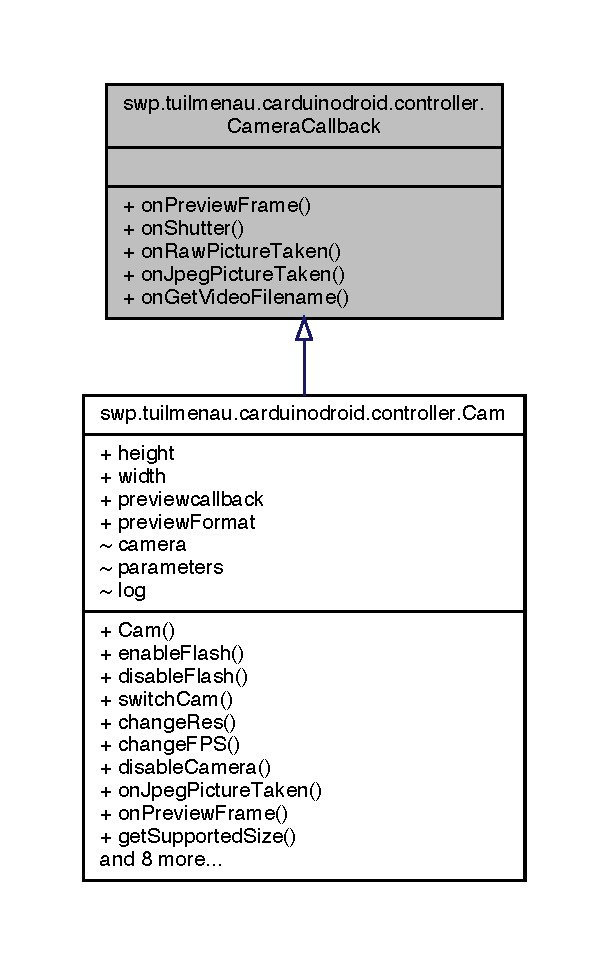
\includegraphics[width=292pt]{interfaceswp_1_1tuilmenau_1_1carduinodroid_1_1controller_1_1_camera_callback__inherit__graph}
\end{center}
\end{figure}


Collaboration diagram for swp.\+tuilmenau.\+carduinodroid.\+controller.\+Camera\+Callback\+:
\nopagebreak
\begin{figure}[H]
\begin{center}
\leavevmode
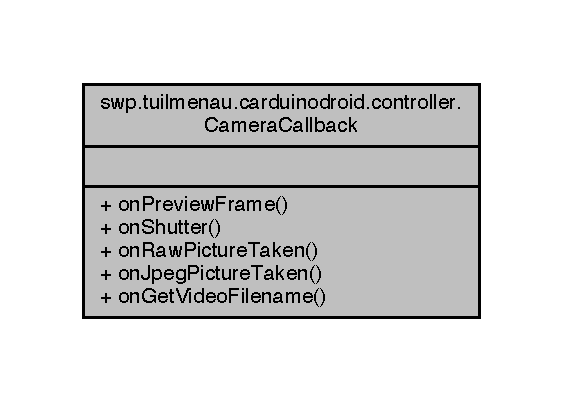
\includegraphics[width=270pt]{interfaceswp_1_1tuilmenau_1_1carduinodroid_1_1controller_1_1_camera_callback__coll__graph}
\end{center}
\end{figure}
\subsection*{Public Member Functions}
\begin{DoxyCompactItemize}
\item 
abstract void \hyperlink{interfaceswp_1_1tuilmenau_1_1carduinodroid_1_1controller_1_1_camera_callback_af289d167147fc931021807a91936ddf9}{on\+Preview\+Frame} (byte\mbox{[}$\,$\mbox{]} data, Camera camera)
\item 
abstract void \hyperlink{interfaceswp_1_1tuilmenau_1_1carduinodroid_1_1controller_1_1_camera_callback_a30aa84ddd47b4a441246873824bfef48}{on\+Shutter} ()
\item 
abstract void \hyperlink{interfaceswp_1_1tuilmenau_1_1carduinodroid_1_1controller_1_1_camera_callback_aa2ac80b68898674885323f6aaeeaf94c}{on\+Raw\+Picture\+Taken} (byte\mbox{[}$\,$\mbox{]} data, Camera camera)
\item 
abstract void \hyperlink{interfaceswp_1_1tuilmenau_1_1carduinodroid_1_1controller_1_1_camera_callback_a5b358bbeb91e1b5b8e3f1dc2ce9fcd95}{on\+Jpeg\+Picture\+Taken} (byte\mbox{[}$\,$\mbox{]} data, Camera camera)
\item 
abstract String \hyperlink{interfaceswp_1_1tuilmenau_1_1carduinodroid_1_1controller_1_1_camera_callback_a5ca843e916557f8e59378fa7dade887a}{on\+Get\+Video\+Filename} ()
\end{DoxyCompactItemize}


\subsection{Detailed Description}
\begin{DoxyAuthor}{Author}
Robin 
\end{DoxyAuthor}
\begin{DoxySeeAlso}{See also}
android.\+hardware.\+Camera.\+Preview\+Callback 

android.\+hardware.\+Camera.\+Shutter\+Callback 

android.\+hardware.\+Camera.\+Picture\+Callback 
\end{DoxySeeAlso}


\subsection{Member Function Documentation}
\hypertarget{interfaceswp_1_1tuilmenau_1_1carduinodroid_1_1controller_1_1_camera_callback_a5ca843e916557f8e59378fa7dade887a}{}\index{swp\+::tuilmenau\+::carduinodroid\+::controller\+::\+Camera\+Callback@{swp\+::tuilmenau\+::carduinodroid\+::controller\+::\+Camera\+Callback}!on\+Get\+Video\+Filename@{on\+Get\+Video\+Filename}}
\index{on\+Get\+Video\+Filename@{on\+Get\+Video\+Filename}!swp\+::tuilmenau\+::carduinodroid\+::controller\+::\+Camera\+Callback@{swp\+::tuilmenau\+::carduinodroid\+::controller\+::\+Camera\+Callback}}
\subsubsection[{on\+Get\+Video\+Filename}]{\setlength{\rightskip}{0pt plus 5cm}abstract String swp.\+tuilmenau.\+carduinodroid.\+controller.\+Camera\+Callback.\+on\+Get\+Video\+Filename (
\begin{DoxyParamCaption}
{}
\end{DoxyParamCaption}
)\hspace{0.3cm}{\ttfamily [abstract]}}\label{interfaceswp_1_1tuilmenau_1_1carduinodroid_1_1controller_1_1_camera_callback_a5ca843e916557f8e59378fa7dade887a}


Implemented in \hyperlink{classswp_1_1tuilmenau_1_1carduinodroid_1_1controller_1_1_cam_a75b628ee85543bcf0a65cacdaa740430}{swp.\+tuilmenau.\+carduinodroid.\+controller.\+Cam}.

\hypertarget{interfaceswp_1_1tuilmenau_1_1carduinodroid_1_1controller_1_1_camera_callback_a5b358bbeb91e1b5b8e3f1dc2ce9fcd95}{}\index{swp\+::tuilmenau\+::carduinodroid\+::controller\+::\+Camera\+Callback@{swp\+::tuilmenau\+::carduinodroid\+::controller\+::\+Camera\+Callback}!on\+Jpeg\+Picture\+Taken@{on\+Jpeg\+Picture\+Taken}}
\index{on\+Jpeg\+Picture\+Taken@{on\+Jpeg\+Picture\+Taken}!swp\+::tuilmenau\+::carduinodroid\+::controller\+::\+Camera\+Callback@{swp\+::tuilmenau\+::carduinodroid\+::controller\+::\+Camera\+Callback}}
\subsubsection[{on\+Jpeg\+Picture\+Taken}]{\setlength{\rightskip}{0pt plus 5cm}abstract void swp.\+tuilmenau.\+carduinodroid.\+controller.\+Camera\+Callback.\+on\+Jpeg\+Picture\+Taken (
\begin{DoxyParamCaption}
\item[{byte\mbox{[}$\,$\mbox{]}}]{data, }
\item[{Camera}]{camera}
\end{DoxyParamCaption}
)\hspace{0.3cm}{\ttfamily [abstract]}}\label{interfaceswp_1_1tuilmenau_1_1carduinodroid_1_1controller_1_1_camera_callback_a5b358bbeb91e1b5b8e3f1dc2ce9fcd95}


Implemented in \hyperlink{classswp_1_1tuilmenau_1_1carduinodroid_1_1controller_1_1_cam_a9d02cf28701a301ae81da9d826b6c6d6}{swp.\+tuilmenau.\+carduinodroid.\+controller.\+Cam}.

\hypertarget{interfaceswp_1_1tuilmenau_1_1carduinodroid_1_1controller_1_1_camera_callback_af289d167147fc931021807a91936ddf9}{}\index{swp\+::tuilmenau\+::carduinodroid\+::controller\+::\+Camera\+Callback@{swp\+::tuilmenau\+::carduinodroid\+::controller\+::\+Camera\+Callback}!on\+Preview\+Frame@{on\+Preview\+Frame}}
\index{on\+Preview\+Frame@{on\+Preview\+Frame}!swp\+::tuilmenau\+::carduinodroid\+::controller\+::\+Camera\+Callback@{swp\+::tuilmenau\+::carduinodroid\+::controller\+::\+Camera\+Callback}}
\subsubsection[{on\+Preview\+Frame}]{\setlength{\rightskip}{0pt plus 5cm}abstract void swp.\+tuilmenau.\+carduinodroid.\+controller.\+Camera\+Callback.\+on\+Preview\+Frame (
\begin{DoxyParamCaption}
\item[{byte\mbox{[}$\,$\mbox{]}}]{data, }
\item[{Camera}]{camera}
\end{DoxyParamCaption}
)\hspace{0.3cm}{\ttfamily [abstract]}}\label{interfaceswp_1_1tuilmenau_1_1carduinodroid_1_1controller_1_1_camera_callback_af289d167147fc931021807a91936ddf9}


Implemented in \hyperlink{classswp_1_1tuilmenau_1_1carduinodroid_1_1controller_1_1_cam_a36c84a09cf6164b9e80426a61a5ec860}{swp.\+tuilmenau.\+carduinodroid.\+controller.\+Cam}.

\hypertarget{interfaceswp_1_1tuilmenau_1_1carduinodroid_1_1controller_1_1_camera_callback_aa2ac80b68898674885323f6aaeeaf94c}{}\index{swp\+::tuilmenau\+::carduinodroid\+::controller\+::\+Camera\+Callback@{swp\+::tuilmenau\+::carduinodroid\+::controller\+::\+Camera\+Callback}!on\+Raw\+Picture\+Taken@{on\+Raw\+Picture\+Taken}}
\index{on\+Raw\+Picture\+Taken@{on\+Raw\+Picture\+Taken}!swp\+::tuilmenau\+::carduinodroid\+::controller\+::\+Camera\+Callback@{swp\+::tuilmenau\+::carduinodroid\+::controller\+::\+Camera\+Callback}}
\subsubsection[{on\+Raw\+Picture\+Taken}]{\setlength{\rightskip}{0pt plus 5cm}abstract void swp.\+tuilmenau.\+carduinodroid.\+controller.\+Camera\+Callback.\+on\+Raw\+Picture\+Taken (
\begin{DoxyParamCaption}
\item[{byte\mbox{[}$\,$\mbox{]}}]{data, }
\item[{Camera}]{camera}
\end{DoxyParamCaption}
)\hspace{0.3cm}{\ttfamily [abstract]}}\label{interfaceswp_1_1tuilmenau_1_1carduinodroid_1_1controller_1_1_camera_callback_aa2ac80b68898674885323f6aaeeaf94c}


Implemented in \hyperlink{classswp_1_1tuilmenau_1_1carduinodroid_1_1controller_1_1_cam_a356797b49cf972aa95148c88702cf81a}{swp.\+tuilmenau.\+carduinodroid.\+controller.\+Cam}.

\hypertarget{interfaceswp_1_1tuilmenau_1_1carduinodroid_1_1controller_1_1_camera_callback_a30aa84ddd47b4a441246873824bfef48}{}\index{swp\+::tuilmenau\+::carduinodroid\+::controller\+::\+Camera\+Callback@{swp\+::tuilmenau\+::carduinodroid\+::controller\+::\+Camera\+Callback}!on\+Shutter@{on\+Shutter}}
\index{on\+Shutter@{on\+Shutter}!swp\+::tuilmenau\+::carduinodroid\+::controller\+::\+Camera\+Callback@{swp\+::tuilmenau\+::carduinodroid\+::controller\+::\+Camera\+Callback}}
\subsubsection[{on\+Shutter}]{\setlength{\rightskip}{0pt plus 5cm}abstract void swp.\+tuilmenau.\+carduinodroid.\+controller.\+Camera\+Callback.\+on\+Shutter (
\begin{DoxyParamCaption}
{}
\end{DoxyParamCaption}
)\hspace{0.3cm}{\ttfamily [abstract]}}\label{interfaceswp_1_1tuilmenau_1_1carduinodroid_1_1controller_1_1_camera_callback_a30aa84ddd47b4a441246873824bfef48}


Implemented in \hyperlink{classswp_1_1tuilmenau_1_1carduinodroid_1_1controller_1_1_cam_aef536a7a7774a554aff67f70c5edd1de}{swp.\+tuilmenau.\+carduinodroid.\+controller.\+Cam}.



The documentation for this interface was generated from the following file\+:\begin{DoxyCompactItemize}
\item 
src/swp/tuilmenau/carduinodroid/controller/\hyperlink{_camera_callback_8java}{Camera\+Callback.\+java}\end{DoxyCompactItemize}

\hypertarget{classswp_1_1tuilmenau_1_1carduinodroid_1_1controller_1_1_camera_preview}{}\section{swp.\+tuilmenau.\+carduinodroid.\+controller.\+Camera\+Preview Class Reference}
\label{classswp_1_1tuilmenau_1_1carduinodroid_1_1controller_1_1_camera_preview}\index{swp.\+tuilmenau.\+carduinodroid.\+controller.\+Camera\+Preview@{swp.\+tuilmenau.\+carduinodroid.\+controller.\+Camera\+Preview}}


Inheritance diagram for swp.\+tuilmenau.\+carduinodroid.\+controller.\+Camera\+Preview\+:
\nopagebreak
\begin{figure}[H]
\begin{center}
\leavevmode
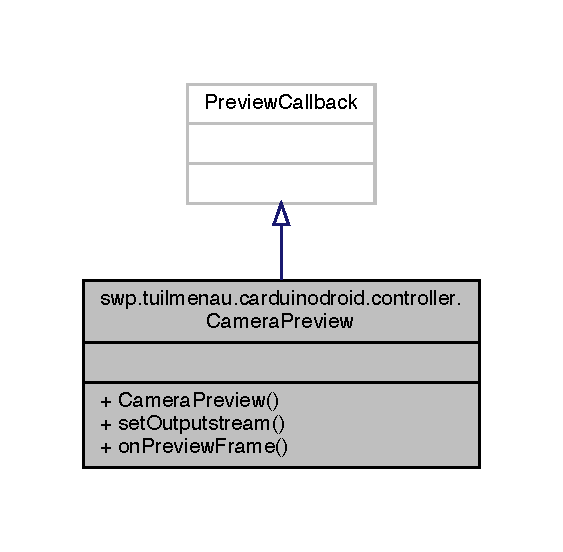
\includegraphics[width=270pt]{classswp_1_1tuilmenau_1_1carduinodroid_1_1controller_1_1_camera_preview__inherit__graph}
\end{center}
\end{figure}


Collaboration diagram for swp.\+tuilmenau.\+carduinodroid.\+controller.\+Camera\+Preview\+:
\nopagebreak
\begin{figure}[H]
\begin{center}
\leavevmode
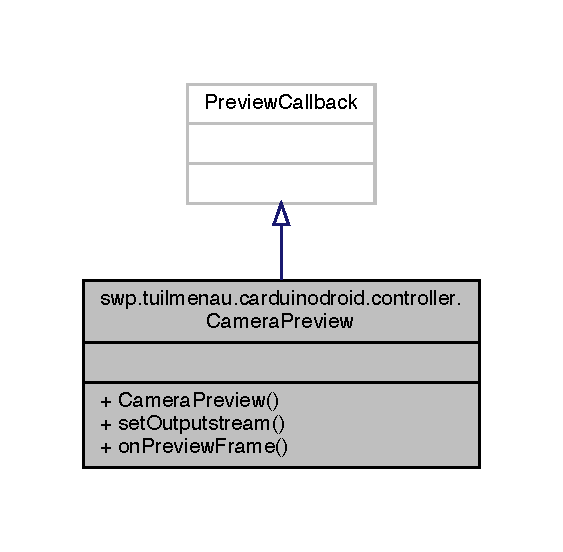
\includegraphics[width=270pt]{classswp_1_1tuilmenau_1_1carduinodroid_1_1controller_1_1_camera_preview__coll__graph}
\end{center}
\end{figure}
\subsection*{Public Member Functions}
\begin{DoxyCompactItemize}
\item 
\hyperlink{classswp_1_1tuilmenau_1_1carduinodroid_1_1controller_1_1_camera_preview_af01876b4b41133af38c837fa10d6d7da}{Camera\+Preview} ()
\item 
void \hyperlink{classswp_1_1tuilmenau_1_1carduinodroid_1_1controller_1_1_camera_preview_a81c06f156a2a06c1463bfdab54dbecfc}{set\+Outputstream} (Output\+Stream noutput\+Stream)
\item 
void \hyperlink{classswp_1_1tuilmenau_1_1carduinodroid_1_1controller_1_1_camera_preview_a171743b48835909ba936b1539e3f63d7}{on\+Preview\+Frame} (byte\mbox{[}$\,$\mbox{]} data, Camera camera)
\end{DoxyCompactItemize}


\subsection{Constructor \& Destructor Documentation}
\hypertarget{classswp_1_1tuilmenau_1_1carduinodroid_1_1controller_1_1_camera_preview_af01876b4b41133af38c837fa10d6d7da}{}\index{swp\+::tuilmenau\+::carduinodroid\+::controller\+::\+Camera\+Preview@{swp\+::tuilmenau\+::carduinodroid\+::controller\+::\+Camera\+Preview}!Camera\+Preview@{Camera\+Preview}}
\index{Camera\+Preview@{Camera\+Preview}!swp\+::tuilmenau\+::carduinodroid\+::controller\+::\+Camera\+Preview@{swp\+::tuilmenau\+::carduinodroid\+::controller\+::\+Camera\+Preview}}
\subsubsection[{Camera\+Preview}]{\setlength{\rightskip}{0pt plus 5cm}swp.\+tuilmenau.\+carduinodroid.\+controller.\+Camera\+Preview.\+Camera\+Preview (
\begin{DoxyParamCaption}
{}
\end{DoxyParamCaption}
)}\label{classswp_1_1tuilmenau_1_1carduinodroid_1_1controller_1_1_camera_preview_af01876b4b41133af38c837fa10d6d7da}


\subsection{Member Function Documentation}
\hypertarget{classswp_1_1tuilmenau_1_1carduinodroid_1_1controller_1_1_camera_preview_a171743b48835909ba936b1539e3f63d7}{}\index{swp\+::tuilmenau\+::carduinodroid\+::controller\+::\+Camera\+Preview@{swp\+::tuilmenau\+::carduinodroid\+::controller\+::\+Camera\+Preview}!on\+Preview\+Frame@{on\+Preview\+Frame}}
\index{on\+Preview\+Frame@{on\+Preview\+Frame}!swp\+::tuilmenau\+::carduinodroid\+::controller\+::\+Camera\+Preview@{swp\+::tuilmenau\+::carduinodroid\+::controller\+::\+Camera\+Preview}}
\subsubsection[{on\+Preview\+Frame}]{\setlength{\rightskip}{0pt plus 5cm}void swp.\+tuilmenau.\+carduinodroid.\+controller.\+Camera\+Preview.\+on\+Preview\+Frame (
\begin{DoxyParamCaption}
\item[{byte\mbox{[}$\,$\mbox{]}}]{data, }
\item[{Camera}]{camera}
\end{DoxyParamCaption}
)}\label{classswp_1_1tuilmenau_1_1carduinodroid_1_1controller_1_1_camera_preview_a171743b48835909ba936b1539e3f63d7}
\hypertarget{classswp_1_1tuilmenau_1_1carduinodroid_1_1controller_1_1_camera_preview_a81c06f156a2a06c1463bfdab54dbecfc}{}\index{swp\+::tuilmenau\+::carduinodroid\+::controller\+::\+Camera\+Preview@{swp\+::tuilmenau\+::carduinodroid\+::controller\+::\+Camera\+Preview}!set\+Outputstream@{set\+Outputstream}}
\index{set\+Outputstream@{set\+Outputstream}!swp\+::tuilmenau\+::carduinodroid\+::controller\+::\+Camera\+Preview@{swp\+::tuilmenau\+::carduinodroid\+::controller\+::\+Camera\+Preview}}
\subsubsection[{set\+Outputstream}]{\setlength{\rightskip}{0pt plus 5cm}void swp.\+tuilmenau.\+carduinodroid.\+controller.\+Camera\+Preview.\+set\+Outputstream (
\begin{DoxyParamCaption}
\item[{Output\+Stream}]{noutput\+Stream}
\end{DoxyParamCaption}
)}\label{classswp_1_1tuilmenau_1_1carduinodroid_1_1controller_1_1_camera_preview_a81c06f156a2a06c1463bfdab54dbecfc}


The documentation for this class was generated from the following file\+:\begin{DoxyCompactItemize}
\item 
src/swp/tuilmenau/carduinodroid/controller/\hyperlink{_camera_preview_8java}{Camera\+Preview.\+java}\end{DoxyCompactItemize}

\hypertarget{classswp_1_1tuilmenau_1_1carduinodroid_1_1controller_1_1_camera_surface}{}\section{swp.\+tuilmenau.\+carduinodroid.\+controller.\+Camera\+Surface Class Reference}
\label{classswp_1_1tuilmenau_1_1carduinodroid_1_1controller_1_1_camera_surface}\index{swp.\+tuilmenau.\+carduinodroid.\+controller.\+Camera\+Surface@{swp.\+tuilmenau.\+carduinodroid.\+controller.\+Camera\+Surface}}


Inheritance diagram for swp.\+tuilmenau.\+carduinodroid.\+controller.\+Camera\+Surface\+:
\nopagebreak
\begin{figure}[H]
\begin{center}
\leavevmode
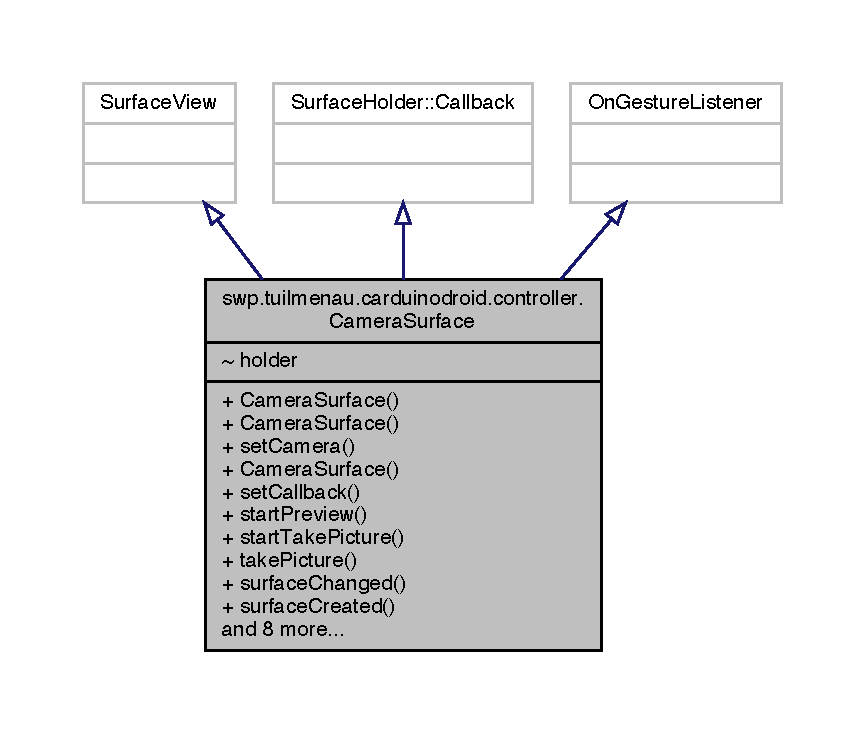
\includegraphics[width=350pt]{classswp_1_1tuilmenau_1_1carduinodroid_1_1controller_1_1_camera_surface__inherit__graph}
\end{center}
\end{figure}


Collaboration diagram for swp.\+tuilmenau.\+carduinodroid.\+controller.\+Camera\+Surface\+:
\nopagebreak
\begin{figure}[H]
\begin{center}
\leavevmode
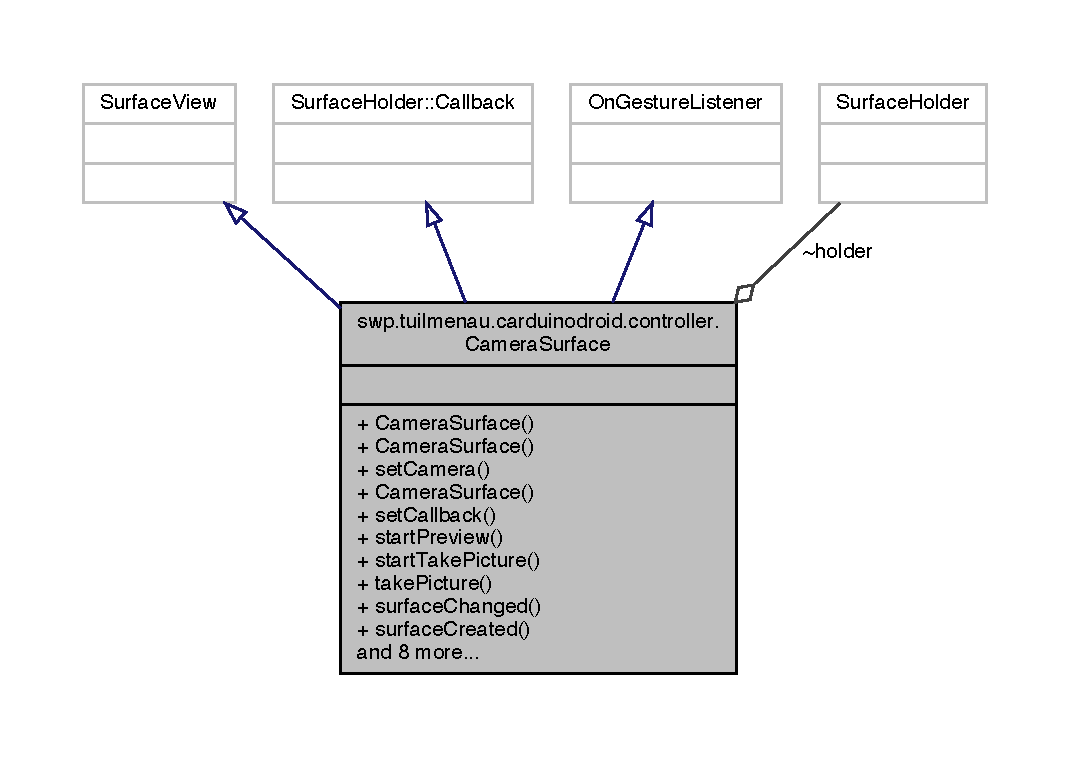
\includegraphics[width=350pt]{classswp_1_1tuilmenau_1_1carduinodroid_1_1controller_1_1_camera_surface__coll__graph}
\end{center}
\end{figure}
\subsection*{Public Member Functions}
\begin{DoxyCompactItemize}
\item 
\hyperlink{classswp_1_1tuilmenau_1_1carduinodroid_1_1controller_1_1_camera_surface_a1c578c6418952fd170916dad67e26152}{Camera\+Surface} (Context context, Attribute\+Set attrs, int def\+Style)
\item 
\hyperlink{classswp_1_1tuilmenau_1_1carduinodroid_1_1controller_1_1_camera_surface_a51856c105777cea804768ed2be7f7aa4}{Camera\+Surface} (Context context, Camera camera, \hyperlink{classswp_1_1tuilmenau_1_1carduinodroid_1_1controller_1_1_cam}{Cam} cam)
\item 
void \hyperlink{classswp_1_1tuilmenau_1_1carduinodroid_1_1controller_1_1_camera_surface_ac0aa798901364be1828f205d940caf4d}{set\+Camera} (Camera camera)
\item 
\hyperlink{classswp_1_1tuilmenau_1_1carduinodroid_1_1controller_1_1_camera_surface_a194d84cc79b5b31f67e620d781438ed3}{Camera\+Surface} (Context context, Attribute\+Set attrs)
\item 
void \hyperlink{classswp_1_1tuilmenau_1_1carduinodroid_1_1controller_1_1_camera_surface_ae9a5ce16713f1cfdb31de1fd212b25e5}{set\+Callback} (\hyperlink{interfaceswp_1_1tuilmenau_1_1carduinodroid_1_1controller_1_1_camera_callback}{Camera\+Callback} callback)
\item 
void \hyperlink{classswp_1_1tuilmenau_1_1carduinodroid_1_1controller_1_1_camera_surface_af09140f0c6c04a3ab83867c9abbd4276}{start\+Preview} ()
\item 
void \hyperlink{classswp_1_1tuilmenau_1_1carduinodroid_1_1controller_1_1_camera_surface_a05163b152120d5aafe3f5d3636d067b3}{start\+Take\+Picture} ()
\item 
void \hyperlink{classswp_1_1tuilmenau_1_1carduinodroid_1_1controller_1_1_camera_surface_a1060767f277e105ef471cc9e299d94bf}{take\+Picture} ()
\item 
void \hyperlink{classswp_1_1tuilmenau_1_1carduinodroid_1_1controller_1_1_camera_surface_a13e24d8a91a594a27cd66f52725de994}{surface\+Changed} (Surface\+Holder holder, int format, int width, int height)
\item 
void \hyperlink{classswp_1_1tuilmenau_1_1carduinodroid_1_1controller_1_1_camera_surface_a714c66493b927383d94a844b742181b8}{surface\+Created} (Surface\+Holder holder)
\item 
void \hyperlink{classswp_1_1tuilmenau_1_1carduinodroid_1_1controller_1_1_camera_surface_ad8a4854496d3186224ff6a86ae1c343c}{surface\+Destroyed} (Surface\+Holder holder)
\item 
boolean \hyperlink{classswp_1_1tuilmenau_1_1carduinodroid_1_1controller_1_1_camera_surface_afd3cacc6c400724abf5c5ded882363b8}{on\+Touch\+Event} (Motion\+Event event)
\item 
boolean \hyperlink{classswp_1_1tuilmenau_1_1carduinodroid_1_1controller_1_1_camera_surface_af54a5e01c5f20ac8212954280c48785a}{on\+Down} (Motion\+Event e)
\item 
boolean \hyperlink{classswp_1_1tuilmenau_1_1carduinodroid_1_1controller_1_1_camera_surface_a2c2c30bc28a1b183bfc3e0492ea1be44}{on\+Fling} (Motion\+Event e1, Motion\+Event e2, float velocity\+X, float velocity\+Y)
\item 
void \hyperlink{classswp_1_1tuilmenau_1_1carduinodroid_1_1controller_1_1_camera_surface_a99ee0d96896cfae8a3be19ce48d61926}{on\+Long\+Press} (Motion\+Event e)
\item 
boolean \hyperlink{classswp_1_1tuilmenau_1_1carduinodroid_1_1controller_1_1_camera_surface_a1cc9dc5983675f90c16b0f64cb322e29}{on\+Scroll} (Motion\+Event e1, Motion\+Event e2, float distance\+X, float distance\+Y)
\item 
void \hyperlink{classswp_1_1tuilmenau_1_1carduinodroid_1_1controller_1_1_camera_surface_ab738bf7ace1ef2c497c39984bb585369}{on\+Show\+Press} (Motion\+Event e)
\item 
boolean \hyperlink{classswp_1_1tuilmenau_1_1carduinodroid_1_1controller_1_1_camera_surface_acc22d3ff51d7099601473ce0a26f7ab5}{on\+Single\+Tap\+Up} (Motion\+Event e)
\end{DoxyCompactItemize}


\subsection{Detailed Description}
\begin{DoxyAuthor}{Author}
Robin 
\end{DoxyAuthor}
\begin{DoxySeeAlso}{See also}
android.\+view.\+Surface\+View 
\end{DoxySeeAlso}


\subsection{Constructor \& Destructor Documentation}
\hypertarget{classswp_1_1tuilmenau_1_1carduinodroid_1_1controller_1_1_camera_surface_a1c578c6418952fd170916dad67e26152}{}\index{swp\+::tuilmenau\+::carduinodroid\+::controller\+::\+Camera\+Surface@{swp\+::tuilmenau\+::carduinodroid\+::controller\+::\+Camera\+Surface}!Camera\+Surface@{Camera\+Surface}}
\index{Camera\+Surface@{Camera\+Surface}!swp\+::tuilmenau\+::carduinodroid\+::controller\+::\+Camera\+Surface@{swp\+::tuilmenau\+::carduinodroid\+::controller\+::\+Camera\+Surface}}
\subsubsection[{Camera\+Surface}]{\setlength{\rightskip}{0pt plus 5cm}swp.\+tuilmenau.\+carduinodroid.\+controller.\+Camera\+Surface.\+Camera\+Surface (
\begin{DoxyParamCaption}
\item[{Context}]{context, }
\item[{Attribute\+Set}]{attrs, }
\item[{int}]{def\+Style}
\end{DoxyParamCaption}
)}\label{classswp_1_1tuilmenau_1_1carduinodroid_1_1controller_1_1_camera_surface_a1c578c6418952fd170916dad67e26152}
Calls the constructor of Surface\+View and initialize the Surface\+Holder 
\begin{DoxyParams}{Parameters}
{\em context} & \\
\hline
{\em attrs} & \\
\hline
{\em def\+Style} & \\
\hline
\end{DoxyParams}
\begin{DoxySeeAlso}{See also}
android.\+view.\+Surface\+View\+::\+Surface\+View(android.\+content.\+Context, android.\+util.\+Attribute\+Set, int) 
\end{DoxySeeAlso}
\hypertarget{classswp_1_1tuilmenau_1_1carduinodroid_1_1controller_1_1_camera_surface_a51856c105777cea804768ed2be7f7aa4}{}\index{swp\+::tuilmenau\+::carduinodroid\+::controller\+::\+Camera\+Surface@{swp\+::tuilmenau\+::carduinodroid\+::controller\+::\+Camera\+Surface}!Camera\+Surface@{Camera\+Surface}}
\index{Camera\+Surface@{Camera\+Surface}!swp\+::tuilmenau\+::carduinodroid\+::controller\+::\+Camera\+Surface@{swp\+::tuilmenau\+::carduinodroid\+::controller\+::\+Camera\+Surface}}
\subsubsection[{Camera\+Surface}]{\setlength{\rightskip}{0pt plus 5cm}swp.\+tuilmenau.\+carduinodroid.\+controller.\+Camera\+Surface.\+Camera\+Surface (
\begin{DoxyParamCaption}
\item[{Context}]{context, }
\item[{Camera}]{camera, }
\item[{{\bf Cam}}]{cam}
\end{DoxyParamCaption}
)}\label{classswp_1_1tuilmenau_1_1carduinodroid_1_1controller_1_1_camera_surface_a51856c105777cea804768ed2be7f7aa4}
Calls the constructor of Surface\+View and initialize the Surface\+Holder 
\begin{DoxyParams}{Parameters}
{\em context} & \\
\hline
{\em camera} & \\
\hline
\end{DoxyParams}
\begin{DoxySeeAlso}{See also}
android.\+view.\+Surface\+View\+::\+Surface\+View(android.\+content.\+Context) 
\end{DoxySeeAlso}
\hypertarget{classswp_1_1tuilmenau_1_1carduinodroid_1_1controller_1_1_camera_surface_a194d84cc79b5b31f67e620d781438ed3}{}\index{swp\+::tuilmenau\+::carduinodroid\+::controller\+::\+Camera\+Surface@{swp\+::tuilmenau\+::carduinodroid\+::controller\+::\+Camera\+Surface}!Camera\+Surface@{Camera\+Surface}}
\index{Camera\+Surface@{Camera\+Surface}!swp\+::tuilmenau\+::carduinodroid\+::controller\+::\+Camera\+Surface@{swp\+::tuilmenau\+::carduinodroid\+::controller\+::\+Camera\+Surface}}
\subsubsection[{Camera\+Surface}]{\setlength{\rightskip}{0pt plus 5cm}swp.\+tuilmenau.\+carduinodroid.\+controller.\+Camera\+Surface.\+Camera\+Surface (
\begin{DoxyParamCaption}
\item[{Context}]{context, }
\item[{Attribute\+Set}]{attrs}
\end{DoxyParamCaption}
)}\label{classswp_1_1tuilmenau_1_1carduinodroid_1_1controller_1_1_camera_surface_a194d84cc79b5b31f67e620d781438ed3}
Calls the constructor of Surface\+View and initialize the Surface\+Holder 
\begin{DoxyParams}{Parameters}
{\em context} & \\
\hline
{\em attrs} & \\
\hline
\end{DoxyParams}
\begin{DoxySeeAlso}{See also}
android.\+view.\+Surface\+View\+::\+Surface\+View(android.\+content.\+Context, android.\+util.\+Attribute\+Set) 
\end{DoxySeeAlso}


\subsection{Member Function Documentation}
\hypertarget{classswp_1_1tuilmenau_1_1carduinodroid_1_1controller_1_1_camera_surface_af54a5e01c5f20ac8212954280c48785a}{}\index{swp\+::tuilmenau\+::carduinodroid\+::controller\+::\+Camera\+Surface@{swp\+::tuilmenau\+::carduinodroid\+::controller\+::\+Camera\+Surface}!on\+Down@{on\+Down}}
\index{on\+Down@{on\+Down}!swp\+::tuilmenau\+::carduinodroid\+::controller\+::\+Camera\+Surface@{swp\+::tuilmenau\+::carduinodroid\+::controller\+::\+Camera\+Surface}}
\subsubsection[{on\+Down}]{\setlength{\rightskip}{0pt plus 5cm}boolean swp.\+tuilmenau.\+carduinodroid.\+controller.\+Camera\+Surface.\+on\+Down (
\begin{DoxyParamCaption}
\item[{Motion\+Event}]{e}
\end{DoxyParamCaption}
)}\label{classswp_1_1tuilmenau_1_1carduinodroid_1_1controller_1_1_camera_surface_af54a5e01c5f20ac8212954280c48785a}
\hypertarget{classswp_1_1tuilmenau_1_1carduinodroid_1_1controller_1_1_camera_surface_a2c2c30bc28a1b183bfc3e0492ea1be44}{}\index{swp\+::tuilmenau\+::carduinodroid\+::controller\+::\+Camera\+Surface@{swp\+::tuilmenau\+::carduinodroid\+::controller\+::\+Camera\+Surface}!on\+Fling@{on\+Fling}}
\index{on\+Fling@{on\+Fling}!swp\+::tuilmenau\+::carduinodroid\+::controller\+::\+Camera\+Surface@{swp\+::tuilmenau\+::carduinodroid\+::controller\+::\+Camera\+Surface}}
\subsubsection[{on\+Fling}]{\setlength{\rightskip}{0pt plus 5cm}boolean swp.\+tuilmenau.\+carduinodroid.\+controller.\+Camera\+Surface.\+on\+Fling (
\begin{DoxyParamCaption}
\item[{Motion\+Event}]{e1, }
\item[{Motion\+Event}]{e2, }
\item[{float}]{velocity\+X, }
\item[{float}]{velocity\+Y}
\end{DoxyParamCaption}
)}\label{classswp_1_1tuilmenau_1_1carduinodroid_1_1controller_1_1_camera_surface_a2c2c30bc28a1b183bfc3e0492ea1be44}
\hypertarget{classswp_1_1tuilmenau_1_1carduinodroid_1_1controller_1_1_camera_surface_a99ee0d96896cfae8a3be19ce48d61926}{}\index{swp\+::tuilmenau\+::carduinodroid\+::controller\+::\+Camera\+Surface@{swp\+::tuilmenau\+::carduinodroid\+::controller\+::\+Camera\+Surface}!on\+Long\+Press@{on\+Long\+Press}}
\index{on\+Long\+Press@{on\+Long\+Press}!swp\+::tuilmenau\+::carduinodroid\+::controller\+::\+Camera\+Surface@{swp\+::tuilmenau\+::carduinodroid\+::controller\+::\+Camera\+Surface}}
\subsubsection[{on\+Long\+Press}]{\setlength{\rightskip}{0pt plus 5cm}void swp.\+tuilmenau.\+carduinodroid.\+controller.\+Camera\+Surface.\+on\+Long\+Press (
\begin{DoxyParamCaption}
\item[{Motion\+Event}]{e}
\end{DoxyParamCaption}
)}\label{classswp_1_1tuilmenau_1_1carduinodroid_1_1controller_1_1_camera_surface_a99ee0d96896cfae8a3be19ce48d61926}


Here is the call graph for this function\+:
\nopagebreak
\begin{figure}[H]
\begin{center}
\leavevmode
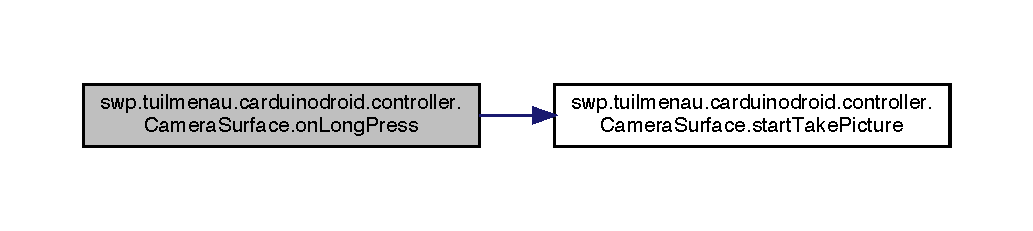
\includegraphics[width=350pt]{classswp_1_1tuilmenau_1_1carduinodroid_1_1controller_1_1_camera_surface_a99ee0d96896cfae8a3be19ce48d61926_cgraph}
\end{center}
\end{figure}


\hypertarget{classswp_1_1tuilmenau_1_1carduinodroid_1_1controller_1_1_camera_surface_a1cc9dc5983675f90c16b0f64cb322e29}{}\index{swp\+::tuilmenau\+::carduinodroid\+::controller\+::\+Camera\+Surface@{swp\+::tuilmenau\+::carduinodroid\+::controller\+::\+Camera\+Surface}!on\+Scroll@{on\+Scroll}}
\index{on\+Scroll@{on\+Scroll}!swp\+::tuilmenau\+::carduinodroid\+::controller\+::\+Camera\+Surface@{swp\+::tuilmenau\+::carduinodroid\+::controller\+::\+Camera\+Surface}}
\subsubsection[{on\+Scroll}]{\setlength{\rightskip}{0pt plus 5cm}boolean swp.\+tuilmenau.\+carduinodroid.\+controller.\+Camera\+Surface.\+on\+Scroll (
\begin{DoxyParamCaption}
\item[{Motion\+Event}]{e1, }
\item[{Motion\+Event}]{e2, }
\item[{float}]{distance\+X, }
\item[{float}]{distance\+Y}
\end{DoxyParamCaption}
)}\label{classswp_1_1tuilmenau_1_1carduinodroid_1_1controller_1_1_camera_surface_a1cc9dc5983675f90c16b0f64cb322e29}
\hypertarget{classswp_1_1tuilmenau_1_1carduinodroid_1_1controller_1_1_camera_surface_ab738bf7ace1ef2c497c39984bb585369}{}\index{swp\+::tuilmenau\+::carduinodroid\+::controller\+::\+Camera\+Surface@{swp\+::tuilmenau\+::carduinodroid\+::controller\+::\+Camera\+Surface}!on\+Show\+Press@{on\+Show\+Press}}
\index{on\+Show\+Press@{on\+Show\+Press}!swp\+::tuilmenau\+::carduinodroid\+::controller\+::\+Camera\+Surface@{swp\+::tuilmenau\+::carduinodroid\+::controller\+::\+Camera\+Surface}}
\subsubsection[{on\+Show\+Press}]{\setlength{\rightskip}{0pt plus 5cm}void swp.\+tuilmenau.\+carduinodroid.\+controller.\+Camera\+Surface.\+on\+Show\+Press (
\begin{DoxyParamCaption}
\item[{Motion\+Event}]{e}
\end{DoxyParamCaption}
)}\label{classswp_1_1tuilmenau_1_1carduinodroid_1_1controller_1_1_camera_surface_ab738bf7ace1ef2c497c39984bb585369}
\hypertarget{classswp_1_1tuilmenau_1_1carduinodroid_1_1controller_1_1_camera_surface_acc22d3ff51d7099601473ce0a26f7ab5}{}\index{swp\+::tuilmenau\+::carduinodroid\+::controller\+::\+Camera\+Surface@{swp\+::tuilmenau\+::carduinodroid\+::controller\+::\+Camera\+Surface}!on\+Single\+Tap\+Up@{on\+Single\+Tap\+Up}}
\index{on\+Single\+Tap\+Up@{on\+Single\+Tap\+Up}!swp\+::tuilmenau\+::carduinodroid\+::controller\+::\+Camera\+Surface@{swp\+::tuilmenau\+::carduinodroid\+::controller\+::\+Camera\+Surface}}
\subsubsection[{on\+Single\+Tap\+Up}]{\setlength{\rightskip}{0pt plus 5cm}boolean swp.\+tuilmenau.\+carduinodroid.\+controller.\+Camera\+Surface.\+on\+Single\+Tap\+Up (
\begin{DoxyParamCaption}
\item[{Motion\+Event}]{e}
\end{DoxyParamCaption}
)}\label{classswp_1_1tuilmenau_1_1carduinodroid_1_1controller_1_1_camera_surface_acc22d3ff51d7099601473ce0a26f7ab5}
\hypertarget{classswp_1_1tuilmenau_1_1carduinodroid_1_1controller_1_1_camera_surface_afd3cacc6c400724abf5c5ded882363b8}{}\index{swp\+::tuilmenau\+::carduinodroid\+::controller\+::\+Camera\+Surface@{swp\+::tuilmenau\+::carduinodroid\+::controller\+::\+Camera\+Surface}!on\+Touch\+Event@{on\+Touch\+Event}}
\index{on\+Touch\+Event@{on\+Touch\+Event}!swp\+::tuilmenau\+::carduinodroid\+::controller\+::\+Camera\+Surface@{swp\+::tuilmenau\+::carduinodroid\+::controller\+::\+Camera\+Surface}}
\subsubsection[{on\+Touch\+Event}]{\setlength{\rightskip}{0pt plus 5cm}boolean swp.\+tuilmenau.\+carduinodroid.\+controller.\+Camera\+Surface.\+on\+Touch\+Event (
\begin{DoxyParamCaption}
\item[{Motion\+Event}]{event}
\end{DoxyParamCaption}
)}\label{classswp_1_1tuilmenau_1_1carduinodroid_1_1controller_1_1_camera_surface_afd3cacc6c400724abf5c5ded882363b8}
\hypertarget{classswp_1_1tuilmenau_1_1carduinodroid_1_1controller_1_1_camera_surface_ae9a5ce16713f1cfdb31de1fd212b25e5}{}\index{swp\+::tuilmenau\+::carduinodroid\+::controller\+::\+Camera\+Surface@{swp\+::tuilmenau\+::carduinodroid\+::controller\+::\+Camera\+Surface}!set\+Callback@{set\+Callback}}
\index{set\+Callback@{set\+Callback}!swp\+::tuilmenau\+::carduinodroid\+::controller\+::\+Camera\+Surface@{swp\+::tuilmenau\+::carduinodroid\+::controller\+::\+Camera\+Surface}}
\subsubsection[{set\+Callback}]{\setlength{\rightskip}{0pt plus 5cm}void swp.\+tuilmenau.\+carduinodroid.\+controller.\+Camera\+Surface.\+set\+Callback (
\begin{DoxyParamCaption}
\item[{{\bf Camera\+Callback}}]{callback}
\end{DoxyParamCaption}
)}\label{classswp_1_1tuilmenau_1_1carduinodroid_1_1controller_1_1_camera_surface_ae9a5ce16713f1cfdb31de1fd212b25e5}
Set the \hyperlink{interfaceswp_1_1tuilmenau_1_1carduinodroid_1_1controller_1_1_camera_callback}{Camera\+Callback} 
\begin{DoxyParams}{Parameters}
{\em callback} & the \hyperlink{interfaceswp_1_1tuilmenau_1_1carduinodroid_1_1controller_1_1_camera_callback}{Camera\+Callback} \\
\hline
\end{DoxyParams}


Here is the caller graph for this function\+:
\nopagebreak
\begin{figure}[H]
\begin{center}
\leavevmode
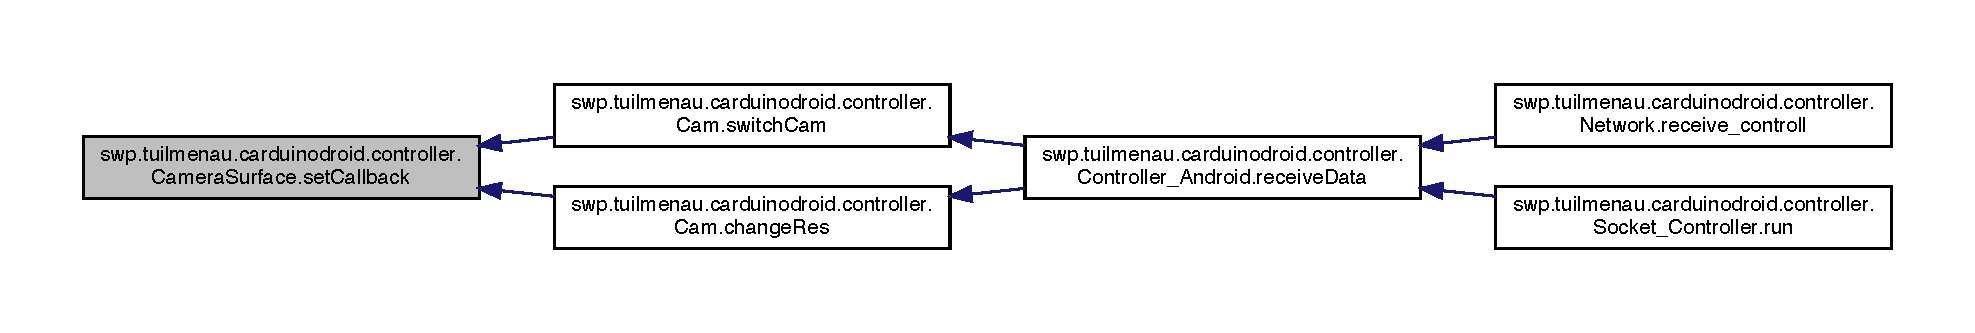
\includegraphics[width=350pt]{classswp_1_1tuilmenau_1_1carduinodroid_1_1controller_1_1_camera_surface_ae9a5ce16713f1cfdb31de1fd212b25e5_icgraph}
\end{center}
\end{figure}


\hypertarget{classswp_1_1tuilmenau_1_1carduinodroid_1_1controller_1_1_camera_surface_ac0aa798901364be1828f205d940caf4d}{}\index{swp\+::tuilmenau\+::carduinodroid\+::controller\+::\+Camera\+Surface@{swp\+::tuilmenau\+::carduinodroid\+::controller\+::\+Camera\+Surface}!set\+Camera@{set\+Camera}}
\index{set\+Camera@{set\+Camera}!swp\+::tuilmenau\+::carduinodroid\+::controller\+::\+Camera\+Surface@{swp\+::tuilmenau\+::carduinodroid\+::controller\+::\+Camera\+Surface}}
\subsubsection[{set\+Camera}]{\setlength{\rightskip}{0pt plus 5cm}void swp.\+tuilmenau.\+carduinodroid.\+controller.\+Camera\+Surface.\+set\+Camera (
\begin{DoxyParamCaption}
\item[{Camera}]{camera}
\end{DoxyParamCaption}
)}\label{classswp_1_1tuilmenau_1_1carduinodroid_1_1controller_1_1_camera_surface_ac0aa798901364be1828f205d940caf4d}


Here is the caller graph for this function\+:
\nopagebreak
\begin{figure}[H]
\begin{center}
\leavevmode
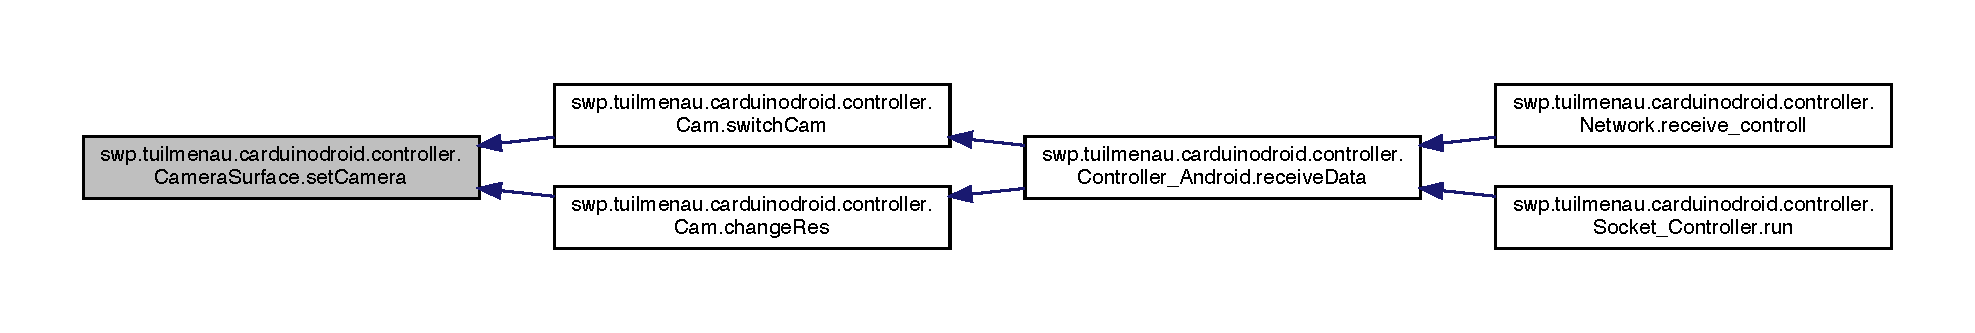
\includegraphics[width=350pt]{classswp_1_1tuilmenau_1_1carduinodroid_1_1controller_1_1_camera_surface_ac0aa798901364be1828f205d940caf4d_icgraph}
\end{center}
\end{figure}


\hypertarget{classswp_1_1tuilmenau_1_1carduinodroid_1_1controller_1_1_camera_surface_af09140f0c6c04a3ab83867c9abbd4276}{}\index{swp\+::tuilmenau\+::carduinodroid\+::controller\+::\+Camera\+Surface@{swp\+::tuilmenau\+::carduinodroid\+::controller\+::\+Camera\+Surface}!start\+Preview@{start\+Preview}}
\index{start\+Preview@{start\+Preview}!swp\+::tuilmenau\+::carduinodroid\+::controller\+::\+Camera\+Surface@{swp\+::tuilmenau\+::carduinodroid\+::controller\+::\+Camera\+Surface}}
\subsubsection[{start\+Preview}]{\setlength{\rightskip}{0pt plus 5cm}void swp.\+tuilmenau.\+carduinodroid.\+controller.\+Camera\+Surface.\+start\+Preview (
\begin{DoxyParamCaption}
{}
\end{DoxyParamCaption}
)}\label{classswp_1_1tuilmenau_1_1carduinodroid_1_1controller_1_1_camera_surface_af09140f0c6c04a3ab83867c9abbd4276}
Starts the Preview \hypertarget{classswp_1_1tuilmenau_1_1carduinodroid_1_1controller_1_1_camera_surface_a05163b152120d5aafe3f5d3636d067b3}{}\index{swp\+::tuilmenau\+::carduinodroid\+::controller\+::\+Camera\+Surface@{swp\+::tuilmenau\+::carduinodroid\+::controller\+::\+Camera\+Surface}!start\+Take\+Picture@{start\+Take\+Picture}}
\index{start\+Take\+Picture@{start\+Take\+Picture}!swp\+::tuilmenau\+::carduinodroid\+::controller\+::\+Camera\+Surface@{swp\+::tuilmenau\+::carduinodroid\+::controller\+::\+Camera\+Surface}}
\subsubsection[{start\+Take\+Picture}]{\setlength{\rightskip}{0pt plus 5cm}void swp.\+tuilmenau.\+carduinodroid.\+controller.\+Camera\+Surface.\+start\+Take\+Picture (
\begin{DoxyParamCaption}
{}
\end{DoxyParamCaption}
)}\label{classswp_1_1tuilmenau_1_1carduinodroid_1_1controller_1_1_camera_surface_a05163b152120d5aafe3f5d3636d067b3}
not used 

Here is the caller graph for this function\+:
\nopagebreak
\begin{figure}[H]
\begin{center}
\leavevmode
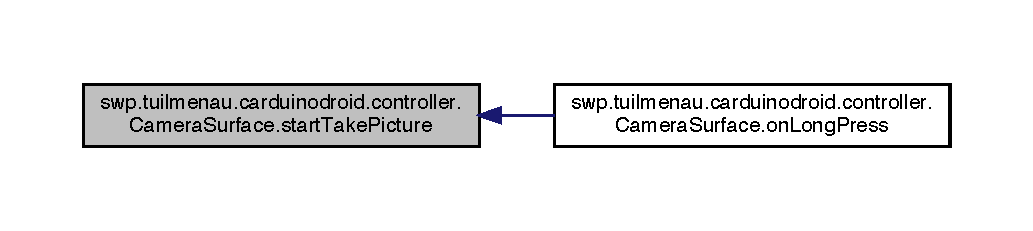
\includegraphics[width=350pt]{classswp_1_1tuilmenau_1_1carduinodroid_1_1controller_1_1_camera_surface_a05163b152120d5aafe3f5d3636d067b3_icgraph}
\end{center}
\end{figure}


\hypertarget{classswp_1_1tuilmenau_1_1carduinodroid_1_1controller_1_1_camera_surface_a13e24d8a91a594a27cd66f52725de994}{}\index{swp\+::tuilmenau\+::carduinodroid\+::controller\+::\+Camera\+Surface@{swp\+::tuilmenau\+::carduinodroid\+::controller\+::\+Camera\+Surface}!surface\+Changed@{surface\+Changed}}
\index{surface\+Changed@{surface\+Changed}!swp\+::tuilmenau\+::carduinodroid\+::controller\+::\+Camera\+Surface@{swp\+::tuilmenau\+::carduinodroid\+::controller\+::\+Camera\+Surface}}
\subsubsection[{surface\+Changed}]{\setlength{\rightskip}{0pt plus 5cm}void swp.\+tuilmenau.\+carduinodroid.\+controller.\+Camera\+Surface.\+surface\+Changed (
\begin{DoxyParamCaption}
\item[{Surface\+Holder}]{holder, }
\item[{int}]{format, }
\item[{int}]{width, }
\item[{int}]{height}
\end{DoxyParamCaption}
)}\label{classswp_1_1tuilmenau_1_1carduinodroid_1_1controller_1_1_camera_surface_a13e24d8a91a594a27cd66f52725de994}
\hypertarget{classswp_1_1tuilmenau_1_1carduinodroid_1_1controller_1_1_camera_surface_a714c66493b927383d94a844b742181b8}{}\index{swp\+::tuilmenau\+::carduinodroid\+::controller\+::\+Camera\+Surface@{swp\+::tuilmenau\+::carduinodroid\+::controller\+::\+Camera\+Surface}!surface\+Created@{surface\+Created}}
\index{surface\+Created@{surface\+Created}!swp\+::tuilmenau\+::carduinodroid\+::controller\+::\+Camera\+Surface@{swp\+::tuilmenau\+::carduinodroid\+::controller\+::\+Camera\+Surface}}
\subsubsection[{surface\+Created}]{\setlength{\rightskip}{0pt plus 5cm}void swp.\+tuilmenau.\+carduinodroid.\+controller.\+Camera\+Surface.\+surface\+Created (
\begin{DoxyParamCaption}
\item[{Surface\+Holder}]{holder}
\end{DoxyParamCaption}
)}\label{classswp_1_1tuilmenau_1_1carduinodroid_1_1controller_1_1_camera_surface_a714c66493b927383d94a844b742181b8}
\hypertarget{classswp_1_1tuilmenau_1_1carduinodroid_1_1controller_1_1_camera_surface_ad8a4854496d3186224ff6a86ae1c343c}{}\index{swp\+::tuilmenau\+::carduinodroid\+::controller\+::\+Camera\+Surface@{swp\+::tuilmenau\+::carduinodroid\+::controller\+::\+Camera\+Surface}!surface\+Destroyed@{surface\+Destroyed}}
\index{surface\+Destroyed@{surface\+Destroyed}!swp\+::tuilmenau\+::carduinodroid\+::controller\+::\+Camera\+Surface@{swp\+::tuilmenau\+::carduinodroid\+::controller\+::\+Camera\+Surface}}
\subsubsection[{surface\+Destroyed}]{\setlength{\rightskip}{0pt plus 5cm}void swp.\+tuilmenau.\+carduinodroid.\+controller.\+Camera\+Surface.\+surface\+Destroyed (
\begin{DoxyParamCaption}
\item[{Surface\+Holder}]{holder}
\end{DoxyParamCaption}
)}\label{classswp_1_1tuilmenau_1_1carduinodroid_1_1controller_1_1_camera_surface_ad8a4854496d3186224ff6a86ae1c343c}
\hypertarget{classswp_1_1tuilmenau_1_1carduinodroid_1_1controller_1_1_camera_surface_a1060767f277e105ef471cc9e299d94bf}{}\index{swp\+::tuilmenau\+::carduinodroid\+::controller\+::\+Camera\+Surface@{swp\+::tuilmenau\+::carduinodroid\+::controller\+::\+Camera\+Surface}!take\+Picture@{take\+Picture}}
\index{take\+Picture@{take\+Picture}!swp\+::tuilmenau\+::carduinodroid\+::controller\+::\+Camera\+Surface@{swp\+::tuilmenau\+::carduinodroid\+::controller\+::\+Camera\+Surface}}
\subsubsection[{take\+Picture}]{\setlength{\rightskip}{0pt plus 5cm}void swp.\+tuilmenau.\+carduinodroid.\+controller.\+Camera\+Surface.\+take\+Picture (
\begin{DoxyParamCaption}
{}
\end{DoxyParamCaption}
)}\label{classswp_1_1tuilmenau_1_1carduinodroid_1_1controller_1_1_camera_surface_a1060767f277e105ef471cc9e299d94bf}
not used 

The documentation for this class was generated from the following file\+:\begin{DoxyCompactItemize}
\item 
src/swp/tuilmenau/carduinodroid/controller/\hyperlink{_camera_surface_8java}{Camera\+Surface.\+java}\end{DoxyCompactItemize}

\hypertarget{classswp_1_1tuilmenau_1_1carduinodroid_1_1_car_duino_droid_app_activity}{}\section{swp.\+tuilmenau.\+carduinodroid.\+Car\+Duino\+Droid\+App\+Activity Class Reference}
\label{classswp_1_1tuilmenau_1_1carduinodroid_1_1_car_duino_droid_app_activity}\index{swp.\+tuilmenau.\+carduinodroid.\+Car\+Duino\+Droid\+App\+Activity@{swp.\+tuilmenau.\+carduinodroid.\+Car\+Duino\+Droid\+App\+Activity}}


Inheritance diagram for swp.\+tuilmenau.\+carduinodroid.\+Car\+Duino\+Droid\+App\+Activity\+:
\nopagebreak
\begin{figure}[H]
\begin{center}
\leavevmode
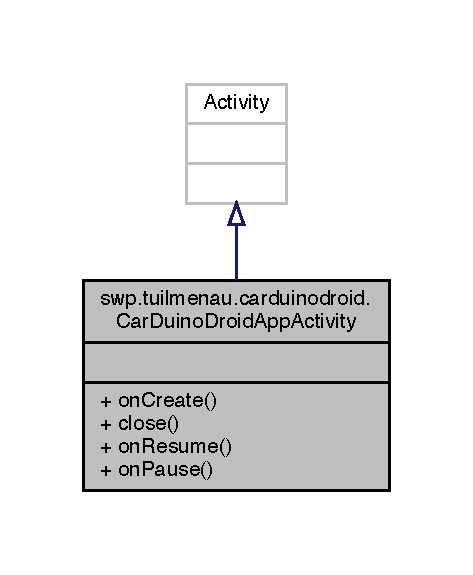
\includegraphics[width=227pt]{classswp_1_1tuilmenau_1_1carduinodroid_1_1_car_duino_droid_app_activity__inherit__graph}
\end{center}
\end{figure}


Collaboration diagram for swp.\+tuilmenau.\+carduinodroid.\+Car\+Duino\+Droid\+App\+Activity\+:
\nopagebreak
\begin{figure}[H]
\begin{center}
\leavevmode
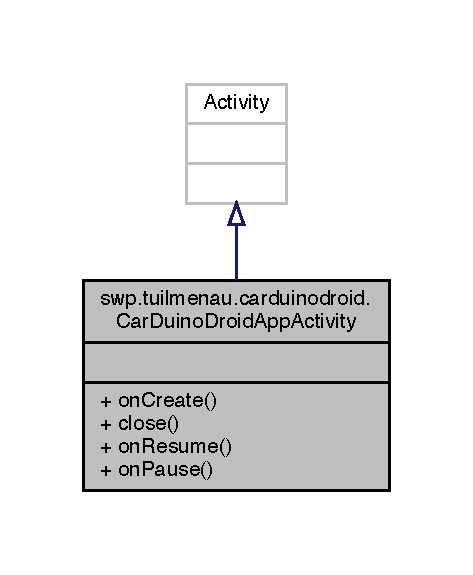
\includegraphics[width=227pt]{classswp_1_1tuilmenau_1_1carduinodroid_1_1_car_duino_droid_app_activity__coll__graph}
\end{center}
\end{figure}
\subsection*{Public Member Functions}
\begin{DoxyCompactItemize}
\item 
void \hyperlink{classswp_1_1tuilmenau_1_1carduinodroid_1_1_car_duino_droid_app_activity_ae4a6735db6fc327f84d1fa9f32d1831c}{on\+Create} (Bundle saved\+Instance\+State)
\item 
void \hyperlink{classswp_1_1tuilmenau_1_1carduinodroid_1_1_car_duino_droid_app_activity_ac44cf73f0d563610f52c55989e0011b2}{close} (View view)
\item 
void \hyperlink{classswp_1_1tuilmenau_1_1carduinodroid_1_1_car_duino_droid_app_activity_aa34abf912f78a88c5c93368fc102e8da}{on\+Resume} ()
\item 
void \hyperlink{classswp_1_1tuilmenau_1_1carduinodroid_1_1_car_duino_droid_app_activity_a019fcfdb908e2fa556d735f477bf8b56}{on\+Pause} ()
\end{DoxyCompactItemize}


\subsection{Detailed Description}
Defines the view presented to the user when opening the App.

\begin{DoxyAuthor}{Author}
Paul Thorwirth 
\end{DoxyAuthor}
\begin{DoxyVersion}{Version}
1.\+0 
\end{DoxyVersion}
\begin{DoxySeeAlso}{See also}
Activity 
\end{DoxySeeAlso}


\subsection{Member Function Documentation}
\hypertarget{classswp_1_1tuilmenau_1_1carduinodroid_1_1_car_duino_droid_app_activity_ac44cf73f0d563610f52c55989e0011b2}{}\index{swp\+::tuilmenau\+::carduinodroid\+::\+Car\+Duino\+Droid\+App\+Activity@{swp\+::tuilmenau\+::carduinodroid\+::\+Car\+Duino\+Droid\+App\+Activity}!close@{close}}
\index{close@{close}!swp\+::tuilmenau\+::carduinodroid\+::\+Car\+Duino\+Droid\+App\+Activity@{swp\+::tuilmenau\+::carduinodroid\+::\+Car\+Duino\+Droid\+App\+Activity}}
\subsubsection[{close}]{\setlength{\rightskip}{0pt plus 5cm}void swp.\+tuilmenau.\+carduinodroid.\+Car\+Duino\+Droid\+App\+Activity.\+close (
\begin{DoxyParamCaption}
\item[{View}]{view}
\end{DoxyParamCaption}
)}\label{classswp_1_1tuilmenau_1_1carduinodroid_1_1_car_duino_droid_app_activity_ac44cf73f0d563610f52c55989e0011b2}
Called when the close button is pressed.


\begin{DoxyParams}{Parameters}
{\em view} & The \hyperlink{}{View} of the button that has been pressed. \\
\hline
\end{DoxyParams}
\begin{DoxySeeAlso}{See also}
Activity\+::finish() 
\end{DoxySeeAlso}
\hypertarget{classswp_1_1tuilmenau_1_1carduinodroid_1_1_car_duino_droid_app_activity_ae4a6735db6fc327f84d1fa9f32d1831c}{}\index{swp\+::tuilmenau\+::carduinodroid\+::\+Car\+Duino\+Droid\+App\+Activity@{swp\+::tuilmenau\+::carduinodroid\+::\+Car\+Duino\+Droid\+App\+Activity}!on\+Create@{on\+Create}}
\index{on\+Create@{on\+Create}!swp\+::tuilmenau\+::carduinodroid\+::\+Car\+Duino\+Droid\+App\+Activity@{swp\+::tuilmenau\+::carduinodroid\+::\+Car\+Duino\+Droid\+App\+Activity}}
\subsubsection[{on\+Create}]{\setlength{\rightskip}{0pt plus 5cm}void swp.\+tuilmenau.\+carduinodroid.\+Car\+Duino\+Droid\+App\+Activity.\+on\+Create (
\begin{DoxyParamCaption}
\item[{Bundle}]{saved\+Instance\+State}
\end{DoxyParamCaption}
)}\label{classswp_1_1tuilmenau_1_1carduinodroid_1_1_car_duino_droid_app_activity_ae4a6735db6fc327f84d1fa9f32d1831c}
Called when the activity is first created.


\begin{DoxyParams}{Parameters}
{\em saved\+Instance\+State} & holds flags and parameters that were saved when the Android System colses the App. \\
\hline
\end{DoxyParams}
\begin{DoxySeeAlso}{See also}
Activity\+::on\+Create() 
\end{DoxySeeAlso}


Here is the call graph for this function\+:
\nopagebreak
\begin{figure}[H]
\begin{center}
\leavevmode
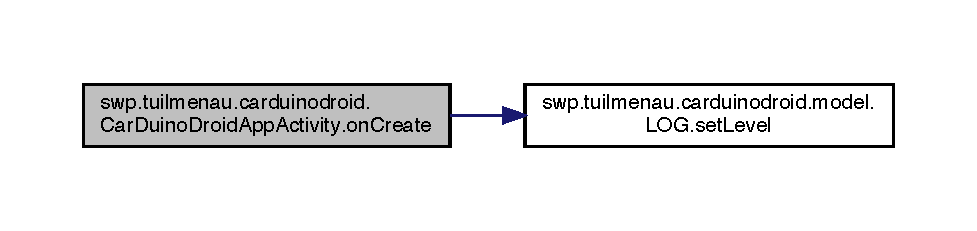
\includegraphics[width=350pt]{classswp_1_1tuilmenau_1_1carduinodroid_1_1_car_duino_droid_app_activity_ae4a6735db6fc327f84d1fa9f32d1831c_cgraph}
\end{center}
\end{figure}


\hypertarget{classswp_1_1tuilmenau_1_1carduinodroid_1_1_car_duino_droid_app_activity_a019fcfdb908e2fa556d735f477bf8b56}{}\index{swp\+::tuilmenau\+::carduinodroid\+::\+Car\+Duino\+Droid\+App\+Activity@{swp\+::tuilmenau\+::carduinodroid\+::\+Car\+Duino\+Droid\+App\+Activity}!on\+Pause@{on\+Pause}}
\index{on\+Pause@{on\+Pause}!swp\+::tuilmenau\+::carduinodroid\+::\+Car\+Duino\+Droid\+App\+Activity@{swp\+::tuilmenau\+::carduinodroid\+::\+Car\+Duino\+Droid\+App\+Activity}}
\subsubsection[{on\+Pause}]{\setlength{\rightskip}{0pt plus 5cm}void swp.\+tuilmenau.\+carduinodroid.\+Car\+Duino\+Droid\+App\+Activity.\+on\+Pause (
\begin{DoxyParamCaption}
{}
\end{DoxyParamCaption}
)}\label{classswp_1_1tuilmenau_1_1carduinodroid_1_1_car_duino_droid_app_activity_a019fcfdb908e2fa556d735f477bf8b56}
Called when the App is minimized.

\begin{DoxySeeAlso}{See also}
Activity\+::on\+Pause() 
\end{DoxySeeAlso}
\hypertarget{classswp_1_1tuilmenau_1_1carduinodroid_1_1_car_duino_droid_app_activity_aa34abf912f78a88c5c93368fc102e8da}{}\index{swp\+::tuilmenau\+::carduinodroid\+::\+Car\+Duino\+Droid\+App\+Activity@{swp\+::tuilmenau\+::carduinodroid\+::\+Car\+Duino\+Droid\+App\+Activity}!on\+Resume@{on\+Resume}}
\index{on\+Resume@{on\+Resume}!swp\+::tuilmenau\+::carduinodroid\+::\+Car\+Duino\+Droid\+App\+Activity@{swp\+::tuilmenau\+::carduinodroid\+::\+Car\+Duino\+Droid\+App\+Activity}}
\subsubsection[{on\+Resume}]{\setlength{\rightskip}{0pt plus 5cm}void swp.\+tuilmenau.\+carduinodroid.\+Car\+Duino\+Droid\+App\+Activity.\+on\+Resume (
\begin{DoxyParamCaption}
{}
\end{DoxyParamCaption}
)}\label{classswp_1_1tuilmenau_1_1carduinodroid_1_1_car_duino_droid_app_activity_aa34abf912f78a88c5c93368fc102e8da}
Called when the activity comes into the foreground.

\begin{DoxySeeAlso}{See also}
Activity\+::on\+Resume() 
\end{DoxySeeAlso}


The documentation for this class was generated from the following file\+:\begin{DoxyCompactItemize}
\item 
src/swp/tuilmenau/carduinodroid/\hyperlink{_car_duino_droid_app_activity_8java}{Car\+Duino\+Droid\+App\+Activity.\+java}\end{DoxyCompactItemize}

\hypertarget{classswp_1_1tuilmenau_1_1carduinodroid_1_1controller_1_1_connection}{}\section{swp.\+tuilmenau.\+carduinodroid.\+controller.\+Connection Class Reference}
\label{classswp_1_1tuilmenau_1_1carduinodroid_1_1controller_1_1_connection}\index{swp.\+tuilmenau.\+carduinodroid.\+controller.\+Connection@{swp.\+tuilmenau.\+carduinodroid.\+controller.\+Connection}}


Collaboration diagram for swp.\+tuilmenau.\+carduinodroid.\+controller.\+Connection\+:
\nopagebreak
\begin{figure}[H]
\begin{center}
\leavevmode
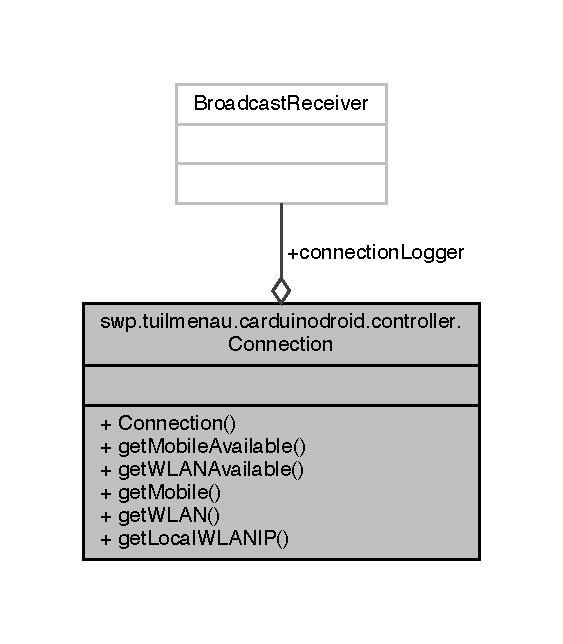
\includegraphics[width=270pt]{classswp_1_1tuilmenau_1_1carduinodroid_1_1controller_1_1_connection__coll__graph}
\end{center}
\end{figure}
\subsection*{Public Member Functions}
\begin{DoxyCompactItemize}
\item 
\hyperlink{classswp_1_1tuilmenau_1_1carduinodroid_1_1controller_1_1_connection_a34bd7c0e4a3a6178864064c97c076adf}{Connection} (Activity activity, \hyperlink{classswp_1_1tuilmenau_1_1carduinodroid_1_1model_1_1_l_o_g}{L\+O\+G} nlog)
\item 
boolean \hyperlink{classswp_1_1tuilmenau_1_1carduinodroid_1_1controller_1_1_connection_ae308ed26606956a787a4b61d3fe7e7a0}{get\+Mobile\+Available} ()
\item 
boolean \hyperlink{classswp_1_1tuilmenau_1_1carduinodroid_1_1controller_1_1_connection_a960f3033213736a2ca426a478ad85a3c}{get\+W\+L\+A\+N\+Available} ()
\item 
boolean \hyperlink{classswp_1_1tuilmenau_1_1carduinodroid_1_1controller_1_1_connection_a3ea65267df8d63ec6a67e511067a674c}{get\+Mobile} ()
\item 
boolean \hyperlink{classswp_1_1tuilmenau_1_1carduinodroid_1_1controller_1_1_connection_acc74178e090418a8ae95b2f2840cf06e}{get\+W\+L\+A\+N} ()
\item 
String \hyperlink{classswp_1_1tuilmenau_1_1carduinodroid_1_1controller_1_1_connection_a478434825ab767b5bf14834a1062abb3}{get\+Local\+W\+L\+A\+N\+I\+P} ()
\end{DoxyCompactItemize}
\subsection*{Public Attributes}
\begin{DoxyCompactItemize}
\item 
Broadcast\+Receiver \hyperlink{classswp_1_1tuilmenau_1_1carduinodroid_1_1controller_1_1_connection_ae6c19aae09ad0cc381b2fd17e5f9cf00}{connection\+Logger}
\end{DoxyCompactItemize}


\subsection{Detailed Description}
Provides an A\+P\+I for handling and changing connection data.

\begin{DoxyAuthor}{Author}
Paul Thorwirth 
\end{DoxyAuthor}
\begin{DoxyVersion}{Version}
1.\+0 
\end{DoxyVersion}
\begin{DoxySeeAlso}{See also}
Connection\+Manager 
\end{DoxySeeAlso}


\subsection{Constructor \& Destructor Documentation}
\hypertarget{classswp_1_1tuilmenau_1_1carduinodroid_1_1controller_1_1_connection_a34bd7c0e4a3a6178864064c97c076adf}{}\index{swp\+::tuilmenau\+::carduinodroid\+::controller\+::\+Connection@{swp\+::tuilmenau\+::carduinodroid\+::controller\+::\+Connection}!Connection@{Connection}}
\index{Connection@{Connection}!swp\+::tuilmenau\+::carduinodroid\+::controller\+::\+Connection@{swp\+::tuilmenau\+::carduinodroid\+::controller\+::\+Connection}}
\subsubsection[{Connection}]{\setlength{\rightskip}{0pt plus 5cm}swp.\+tuilmenau.\+carduinodroid.\+controller.\+Connection.\+Connection (
\begin{DoxyParamCaption}
\item[{Activity}]{activity, }
\item[{{\bf L\+O\+G}}]{nlog}
\end{DoxyParamCaption}
)}\label{classswp_1_1tuilmenau_1_1carduinodroid_1_1controller_1_1_connection_a34bd7c0e4a3a6178864064c97c076adf}
Retrieves an Instance of the Connectivity\+Manager and registers a Broadcast\+Reciever to react on Connectivity-\/\+Events


\begin{DoxyParams}{Parameters}
{\em activity} & The current Activity \\
\hline
{\em nlog} & The Log \\
\hline
\end{DoxyParams}


Here is the call graph for this function\+:
\nopagebreak
\begin{figure}[H]
\begin{center}
\leavevmode
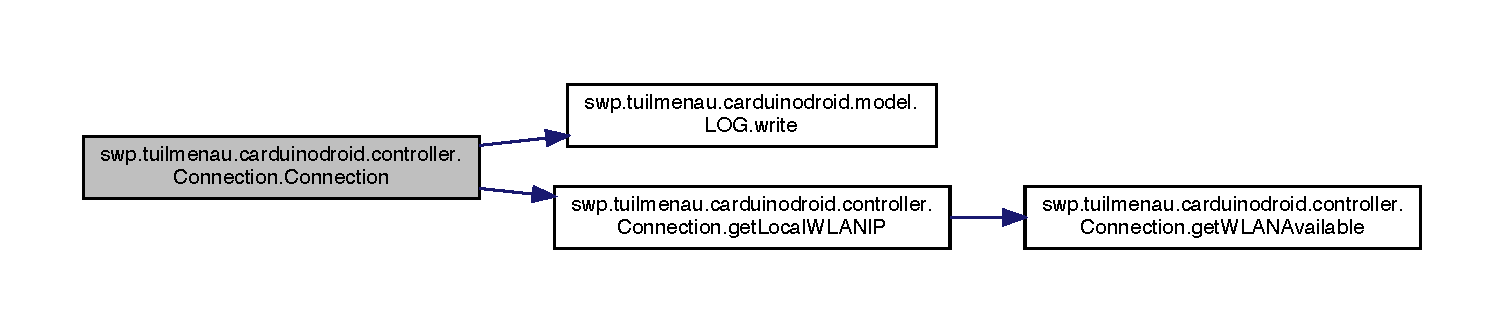
\includegraphics[width=350pt]{classswp_1_1tuilmenau_1_1carduinodroid_1_1controller_1_1_connection_a34bd7c0e4a3a6178864064c97c076adf_cgraph}
\end{center}
\end{figure}




\subsection{Member Function Documentation}
\hypertarget{classswp_1_1tuilmenau_1_1carduinodroid_1_1controller_1_1_connection_a478434825ab767b5bf14834a1062abb3}{}\index{swp\+::tuilmenau\+::carduinodroid\+::controller\+::\+Connection@{swp\+::tuilmenau\+::carduinodroid\+::controller\+::\+Connection}!get\+Local\+W\+L\+A\+N\+I\+P@{get\+Local\+W\+L\+A\+N\+I\+P}}
\index{get\+Local\+W\+L\+A\+N\+I\+P@{get\+Local\+W\+L\+A\+N\+I\+P}!swp\+::tuilmenau\+::carduinodroid\+::controller\+::\+Connection@{swp\+::tuilmenau\+::carduinodroid\+::controller\+::\+Connection}}
\subsubsection[{get\+Local\+W\+L\+A\+N\+I\+P}]{\setlength{\rightskip}{0pt plus 5cm}String swp.\+tuilmenau.\+carduinodroid.\+controller.\+Connection.\+get\+Local\+W\+L\+A\+N\+I\+P (
\begin{DoxyParamCaption}
{}
\end{DoxyParamCaption}
)}\label{classswp_1_1tuilmenau_1_1carduinodroid_1_1controller_1_1_connection_a478434825ab767b5bf14834a1062abb3}
Returns a String representing the current local I\+P of the Phone.

\begin{DoxyReturn}{Returns}
\hyperlink{}{String} representing the current local W\+L\+A\+N I\+P of the Phone. 
\end{DoxyReturn}


Here is the call graph for this function\+:
\nopagebreak
\begin{figure}[H]
\begin{center}
\leavevmode
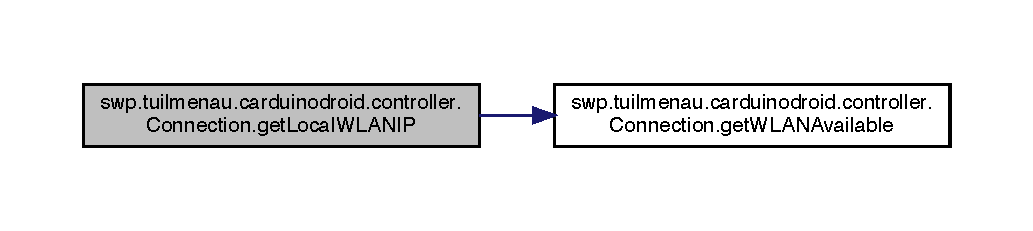
\includegraphics[width=350pt]{classswp_1_1tuilmenau_1_1carduinodroid_1_1controller_1_1_connection_a478434825ab767b5bf14834a1062abb3_cgraph}
\end{center}
\end{figure}




Here is the caller graph for this function\+:
\nopagebreak
\begin{figure}[H]
\begin{center}
\leavevmode
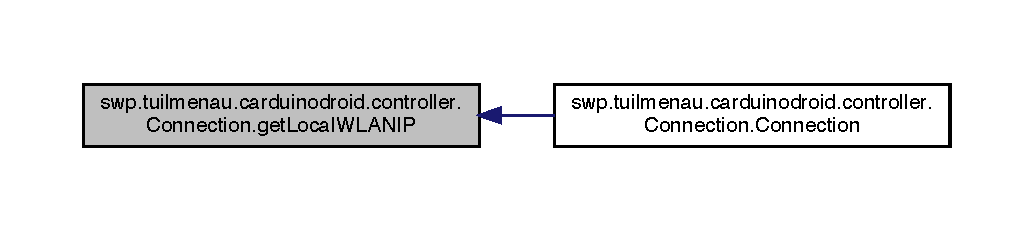
\includegraphics[width=350pt]{classswp_1_1tuilmenau_1_1carduinodroid_1_1controller_1_1_connection_a478434825ab767b5bf14834a1062abb3_icgraph}
\end{center}
\end{figure}


\hypertarget{classswp_1_1tuilmenau_1_1carduinodroid_1_1controller_1_1_connection_a3ea65267df8d63ec6a67e511067a674c}{}\index{swp\+::tuilmenau\+::carduinodroid\+::controller\+::\+Connection@{swp\+::tuilmenau\+::carduinodroid\+::controller\+::\+Connection}!get\+Mobile@{get\+Mobile}}
\index{get\+Mobile@{get\+Mobile}!swp\+::tuilmenau\+::carduinodroid\+::controller\+::\+Connection@{swp\+::tuilmenau\+::carduinodroid\+::controller\+::\+Connection}}
\subsubsection[{get\+Mobile}]{\setlength{\rightskip}{0pt plus 5cm}boolean swp.\+tuilmenau.\+carduinodroid.\+controller.\+Connection.\+get\+Mobile (
\begin{DoxyParamCaption}
{}
\end{DoxyParamCaption}
)}\label{classswp_1_1tuilmenau_1_1carduinodroid_1_1controller_1_1_connection_a3ea65267df8d63ec6a67e511067a674c}
Returns true if there is a mobile Internet is connected.

\begin{DoxyReturn}{Returns}
true if connected false if else. 
\end{DoxyReturn}


Here is the caller graph for this function\+:
\nopagebreak
\begin{figure}[H]
\begin{center}
\leavevmode
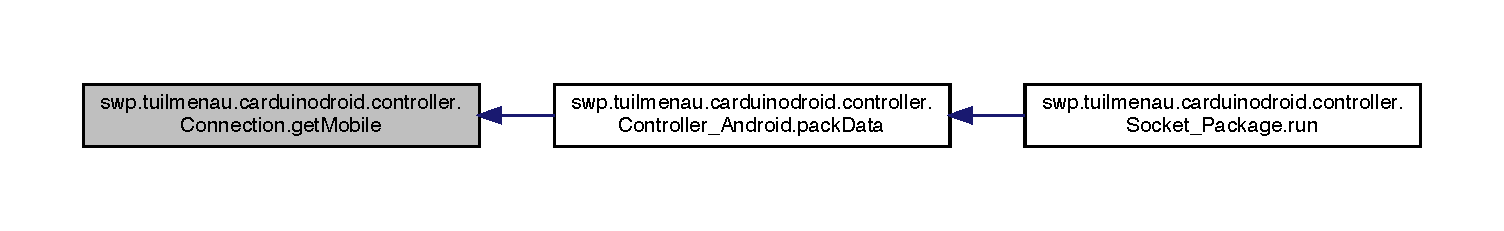
\includegraphics[width=350pt]{classswp_1_1tuilmenau_1_1carduinodroid_1_1controller_1_1_connection_a3ea65267df8d63ec6a67e511067a674c_icgraph}
\end{center}
\end{figure}


\hypertarget{classswp_1_1tuilmenau_1_1carduinodroid_1_1controller_1_1_connection_ae308ed26606956a787a4b61d3fe7e7a0}{}\index{swp\+::tuilmenau\+::carduinodroid\+::controller\+::\+Connection@{swp\+::tuilmenau\+::carduinodroid\+::controller\+::\+Connection}!get\+Mobile\+Available@{get\+Mobile\+Available}}
\index{get\+Mobile\+Available@{get\+Mobile\+Available}!swp\+::tuilmenau\+::carduinodroid\+::controller\+::\+Connection@{swp\+::tuilmenau\+::carduinodroid\+::controller\+::\+Connection}}
\subsubsection[{get\+Mobile\+Available}]{\setlength{\rightskip}{0pt plus 5cm}boolean swp.\+tuilmenau.\+carduinodroid.\+controller.\+Connection.\+get\+Mobile\+Available (
\begin{DoxyParamCaption}
{}
\end{DoxyParamCaption}
)}\label{classswp_1_1tuilmenau_1_1carduinodroid_1_1controller_1_1_connection_ae308ed26606956a787a4b61d3fe7e7a0}
Returns the status on the mobile Internet connection.

\begin{DoxyReturn}{Returns}
true if available false if else. 
\end{DoxyReturn}


Here is the caller graph for this function\+:
\nopagebreak
\begin{figure}[H]
\begin{center}
\leavevmode
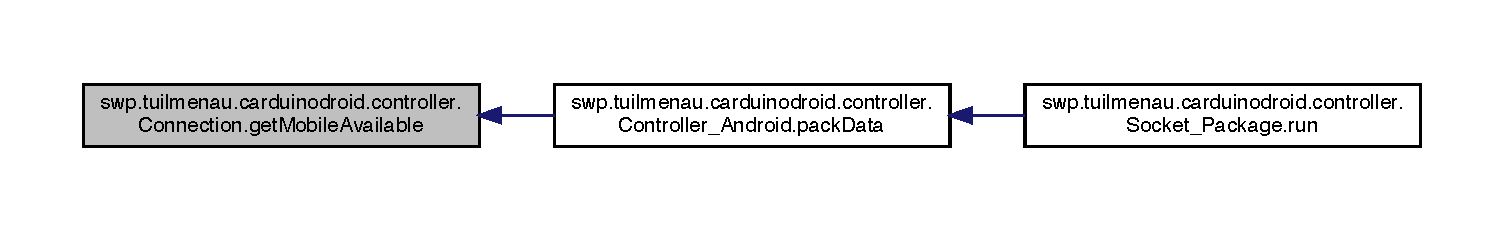
\includegraphics[width=350pt]{classswp_1_1tuilmenau_1_1carduinodroid_1_1controller_1_1_connection_ae308ed26606956a787a4b61d3fe7e7a0_icgraph}
\end{center}
\end{figure}


\hypertarget{classswp_1_1tuilmenau_1_1carduinodroid_1_1controller_1_1_connection_acc74178e090418a8ae95b2f2840cf06e}{}\index{swp\+::tuilmenau\+::carduinodroid\+::controller\+::\+Connection@{swp\+::tuilmenau\+::carduinodroid\+::controller\+::\+Connection}!get\+W\+L\+A\+N@{get\+W\+L\+A\+N}}
\index{get\+W\+L\+A\+N@{get\+W\+L\+A\+N}!swp\+::tuilmenau\+::carduinodroid\+::controller\+::\+Connection@{swp\+::tuilmenau\+::carduinodroid\+::controller\+::\+Connection}}
\subsubsection[{get\+W\+L\+A\+N}]{\setlength{\rightskip}{0pt plus 5cm}boolean swp.\+tuilmenau.\+carduinodroid.\+controller.\+Connection.\+get\+W\+L\+A\+N (
\begin{DoxyParamCaption}
{}
\end{DoxyParamCaption}
)}\label{classswp_1_1tuilmenau_1_1carduinodroid_1_1controller_1_1_connection_acc74178e090418a8ae95b2f2840cf06e}
Returns true if there is a W\+L\+A\+N is connected.

\begin{DoxyReturn}{Returns}
true if connected false if else. 
\end{DoxyReturn}


Here is the caller graph for this function\+:
\nopagebreak
\begin{figure}[H]
\begin{center}
\leavevmode
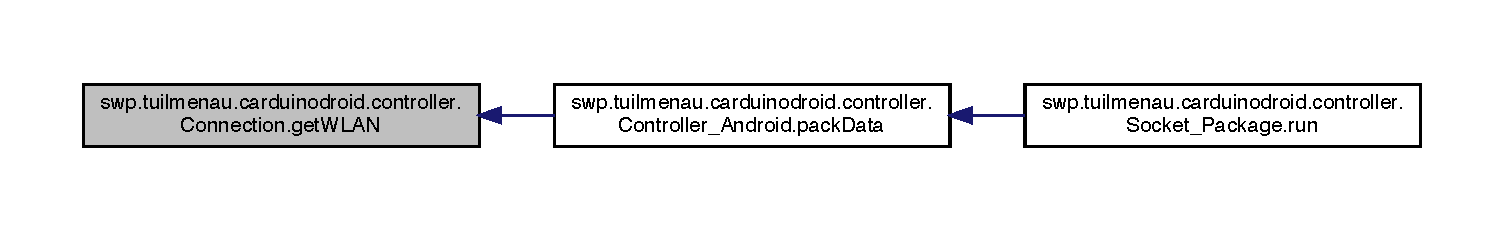
\includegraphics[width=350pt]{classswp_1_1tuilmenau_1_1carduinodroid_1_1controller_1_1_connection_acc74178e090418a8ae95b2f2840cf06e_icgraph}
\end{center}
\end{figure}


\hypertarget{classswp_1_1tuilmenau_1_1carduinodroid_1_1controller_1_1_connection_a960f3033213736a2ca426a478ad85a3c}{}\index{swp\+::tuilmenau\+::carduinodroid\+::controller\+::\+Connection@{swp\+::tuilmenau\+::carduinodroid\+::controller\+::\+Connection}!get\+W\+L\+A\+N\+Available@{get\+W\+L\+A\+N\+Available}}
\index{get\+W\+L\+A\+N\+Available@{get\+W\+L\+A\+N\+Available}!swp\+::tuilmenau\+::carduinodroid\+::controller\+::\+Connection@{swp\+::tuilmenau\+::carduinodroid\+::controller\+::\+Connection}}
\subsubsection[{get\+W\+L\+A\+N\+Available}]{\setlength{\rightskip}{0pt plus 5cm}boolean swp.\+tuilmenau.\+carduinodroid.\+controller.\+Connection.\+get\+W\+L\+A\+N\+Available (
\begin{DoxyParamCaption}
{}
\end{DoxyParamCaption}
)}\label{classswp_1_1tuilmenau_1_1carduinodroid_1_1controller_1_1_connection_a960f3033213736a2ca426a478ad85a3c}
Returns true if there is a W\+L\+A\+N available.

\begin{DoxyReturn}{Returns}
true if available false if else. 
\end{DoxyReturn}


Here is the caller graph for this function\+:
\nopagebreak
\begin{figure}[H]
\begin{center}
\leavevmode
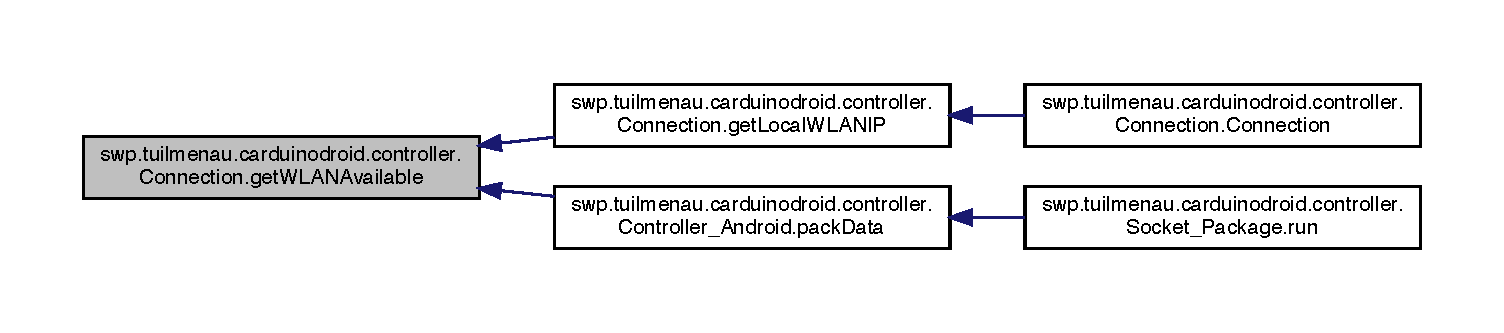
\includegraphics[width=350pt]{classswp_1_1tuilmenau_1_1carduinodroid_1_1controller_1_1_connection_a960f3033213736a2ca426a478ad85a3c_icgraph}
\end{center}
\end{figure}




\subsection{Member Data Documentation}
\hypertarget{classswp_1_1tuilmenau_1_1carduinodroid_1_1controller_1_1_connection_ae6c19aae09ad0cc381b2fd17e5f9cf00}{}\index{swp\+::tuilmenau\+::carduinodroid\+::controller\+::\+Connection@{swp\+::tuilmenau\+::carduinodroid\+::controller\+::\+Connection}!connection\+Logger@{connection\+Logger}}
\index{connection\+Logger@{connection\+Logger}!swp\+::tuilmenau\+::carduinodroid\+::controller\+::\+Connection@{swp\+::tuilmenau\+::carduinodroid\+::controller\+::\+Connection}}
\subsubsection[{connection\+Logger}]{\setlength{\rightskip}{0pt plus 5cm}Broadcast\+Receiver swp.\+tuilmenau.\+carduinodroid.\+controller.\+Connection.\+connection\+Logger}\label{classswp_1_1tuilmenau_1_1carduinodroid_1_1controller_1_1_connection_ae6c19aae09ad0cc381b2fd17e5f9cf00}


The documentation for this class was generated from the following file\+:\begin{DoxyCompactItemize}
\item 
src/swp/tuilmenau/carduinodroid/controller/\hyperlink{_connection_8java}{Connection.\+java}\end{DoxyCompactItemize}

\hypertarget{classswp_1_1tuilmenau_1_1carduinodroid_1_1controller_1_1_controller___android}{}\section{swp.\+tuilmenau.\+carduinodroid.\+controller.\+Controller\+\_\+\+Android Class Reference}
\label{classswp_1_1tuilmenau_1_1carduinodroid_1_1controller_1_1_controller___android}\index{swp.\+tuilmenau.\+carduinodroid.\+controller.\+Controller\+\_\+\+Android@{swp.\+tuilmenau.\+carduinodroid.\+controller.\+Controller\+\_\+\+Android}}


Collaboration diagram for swp.\+tuilmenau.\+carduinodroid.\+controller.\+Controller\+\_\+\+Android\+:
\nopagebreak
\begin{figure}[H]
\begin{center}
\leavevmode
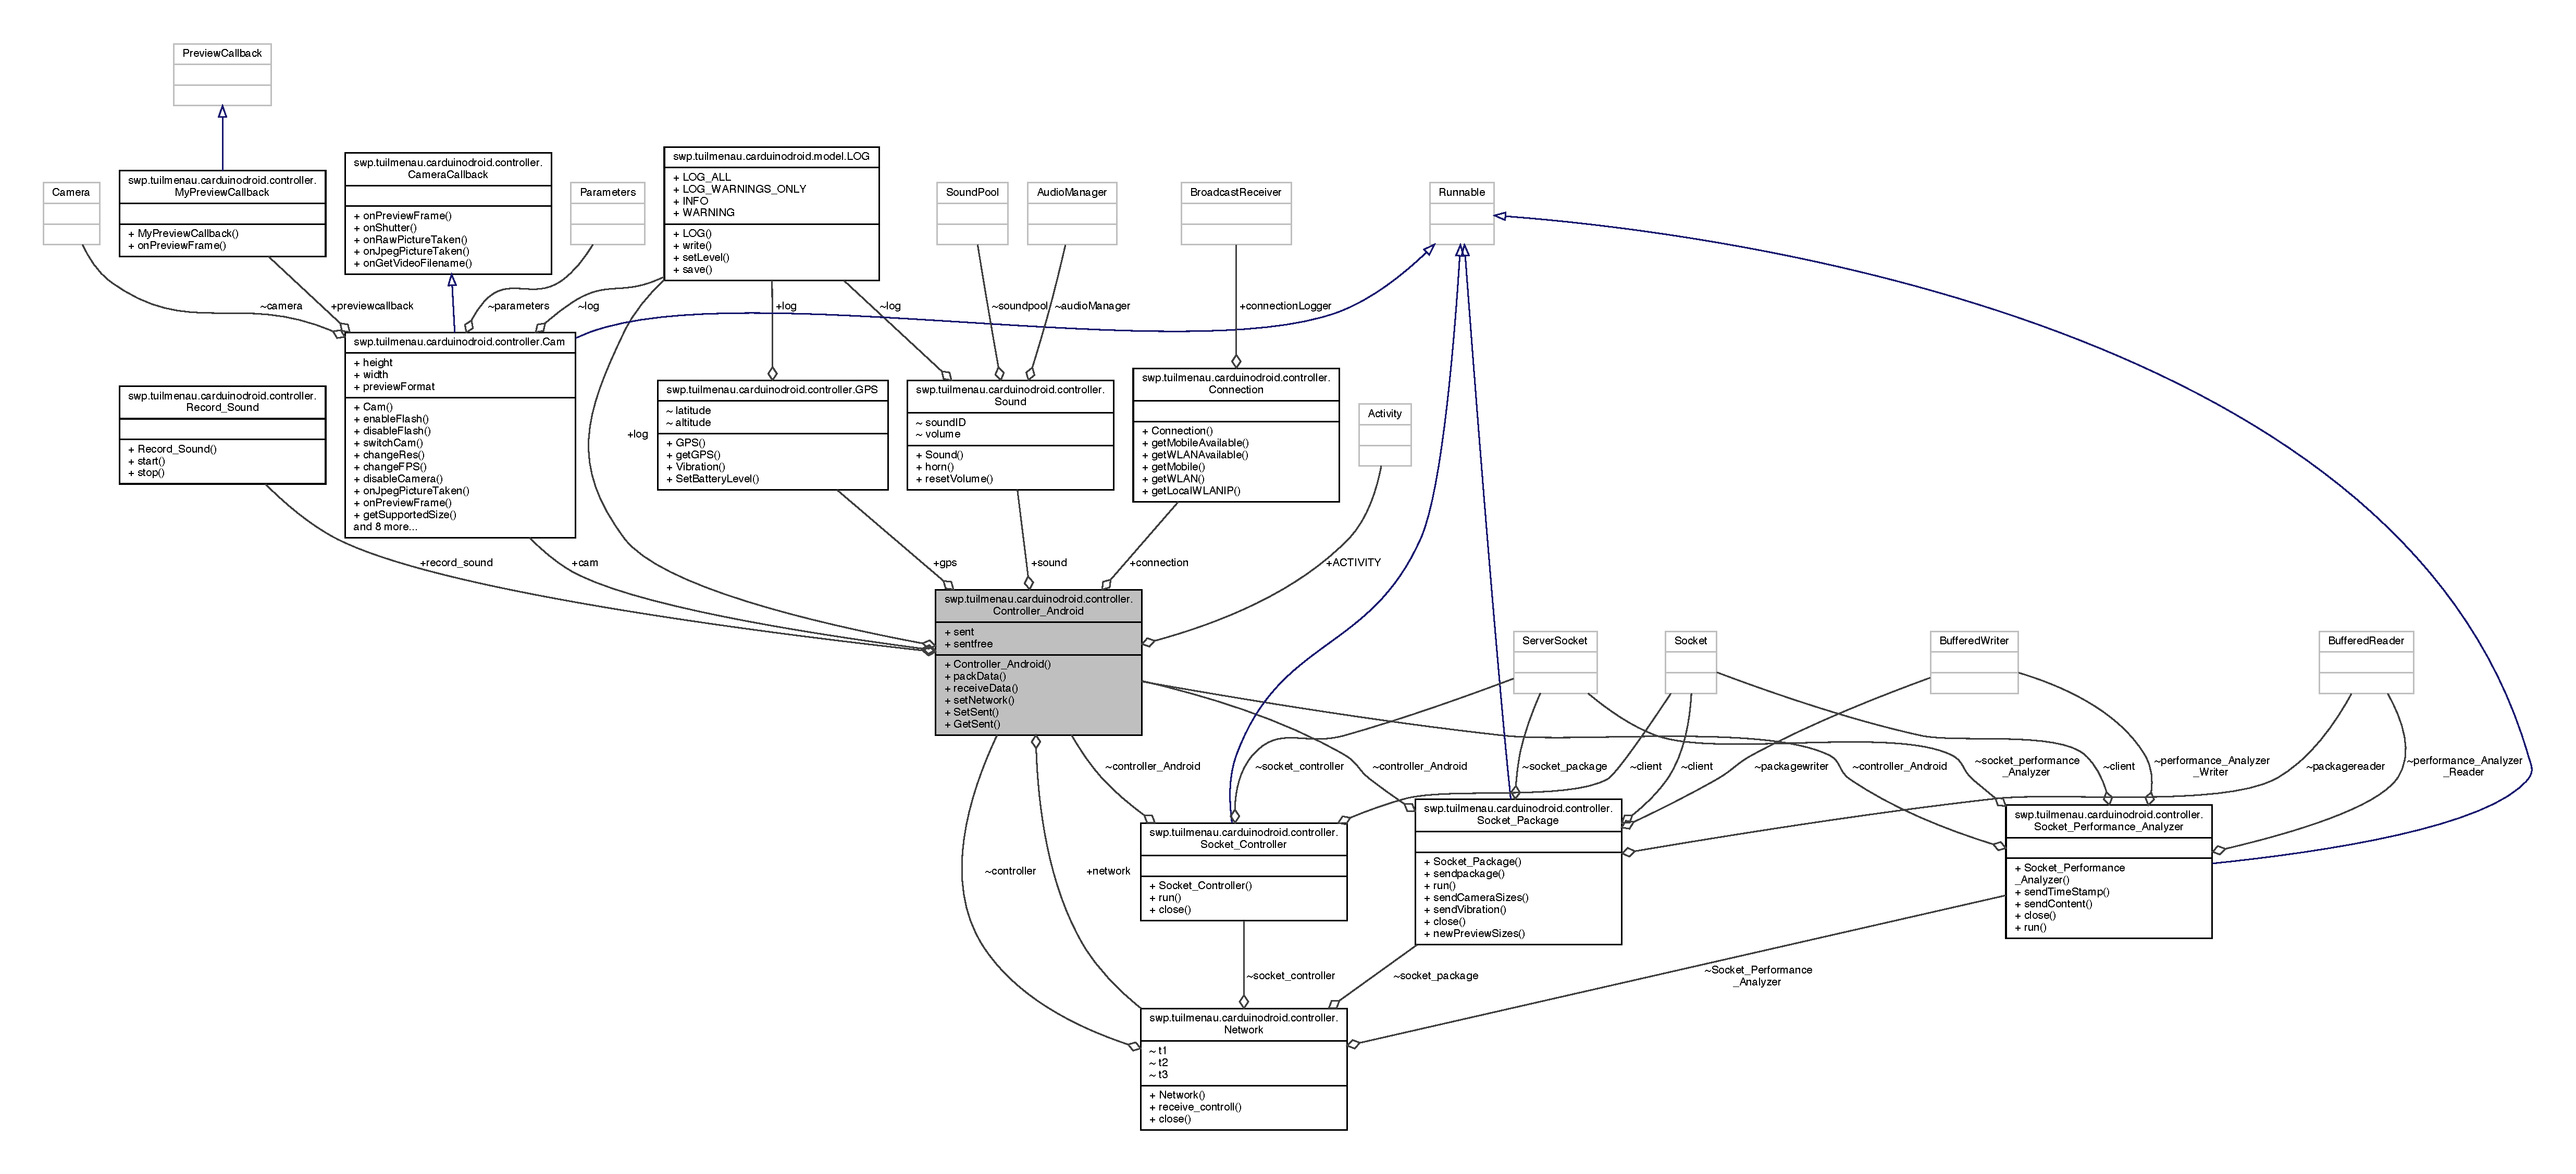
\includegraphics[width=350pt]{classswp_1_1tuilmenau_1_1carduinodroid_1_1controller_1_1_controller___android__coll__graph}
\end{center}
\end{figure}
\subsection*{Public Member Functions}
\begin{DoxyCompactItemize}
\item 
\hyperlink{classswp_1_1tuilmenau_1_1carduinodroid_1_1controller_1_1_controller___android_adf73ebedd13a290596953bc235ac73ba}{Controller\+\_\+\+Android} (Activity activity)
\item 
String \hyperlink{classswp_1_1tuilmenau_1_1carduinodroid_1_1controller_1_1_controller___android_ac8e21f14d9ed1c31500904a4f2a89242}{pack\+Data} ()
\item 
void \hyperlink{classswp_1_1tuilmenau_1_1carduinodroid_1_1controller_1_1_controller___android_aee7580998e493c8fafa0ddd0dff31704}{receive\+Data} (String data)
\item 
void \hyperlink{classswp_1_1tuilmenau_1_1carduinodroid_1_1controller_1_1_controller___android_ae6de91d0d2653cfd019a473cfe8714a1}{set\+Network} (\hyperlink{classswp_1_1tuilmenau_1_1carduinodroid_1_1controller_1_1_network}{Network} \hyperlink{classswp_1_1tuilmenau_1_1carduinodroid_1_1controller_1_1_controller___android_af9cb0b01ab817f064e722a70b0a07987}{network})
\item 
void \hyperlink{classswp_1_1tuilmenau_1_1carduinodroid_1_1controller_1_1_controller___android_aa5f10c125c12e42da6b8eec6d922c7d1}{Set\+Sent} (boolean Sent)
\item 
boolean \hyperlink{classswp_1_1tuilmenau_1_1carduinodroid_1_1controller_1_1_controller___android_ad9b71a18c5f0c004ced9b939c144a3da}{Get\+Sent} ()
\end{DoxyCompactItemize}
\subsection*{Public Attributes}
\begin{DoxyCompactItemize}
\item 
\hyperlink{classswp_1_1tuilmenau_1_1carduinodroid_1_1model_1_1_l_o_g}{L\+O\+G} \hyperlink{classswp_1_1tuilmenau_1_1carduinodroid_1_1controller_1_1_controller___android_affcd564aa1e60c3f85bc6a28864c1d34}{log}
\item 
\hyperlink{classswp_1_1tuilmenau_1_1carduinodroid_1_1controller_1_1_cam}{Cam} \hyperlink{classswp_1_1tuilmenau_1_1carduinodroid_1_1controller_1_1_controller___android_a31da0a49fe10962abd4aa0322e9f30d0}{cam}
\item 
\hyperlink{classswp_1_1tuilmenau_1_1carduinodroid_1_1controller_1_1_connection}{Connection} \hyperlink{classswp_1_1tuilmenau_1_1carduinodroid_1_1controller_1_1_controller___android_a3058848b90ad1bda3b7d9d873e28ac42}{connection}
\item 
\hyperlink{classswp_1_1tuilmenau_1_1carduinodroid_1_1controller_1_1_g_p_s}{G\+P\+S} \hyperlink{classswp_1_1tuilmenau_1_1carduinodroid_1_1controller_1_1_controller___android_ad9f00966717e095bf966440a3d3f2df0}{gps}
\item 
\hyperlink{classswp_1_1tuilmenau_1_1carduinodroid_1_1controller_1_1_network}{Network} \hyperlink{classswp_1_1tuilmenau_1_1carduinodroid_1_1controller_1_1_controller___android_af9cb0b01ab817f064e722a70b0a07987}{network}
\item 
\hyperlink{classswp_1_1tuilmenau_1_1carduinodroid_1_1controller_1_1_record___sound}{Record\+\_\+\+Sound} \hyperlink{classswp_1_1tuilmenau_1_1carduinodroid_1_1controller_1_1_controller___android_a72ea9edd25ca9ef34e5cc7d0facbcd28}{record\+\_\+sound}
\item 
\hyperlink{classswp_1_1tuilmenau_1_1carduinodroid_1_1controller_1_1_sound}{Sound} \hyperlink{classswp_1_1tuilmenau_1_1carduinodroid_1_1controller_1_1_controller___android_af52db04dd80233d572b0fd66e1cf224f}{sound}
\item 
Activity \hyperlink{classswp_1_1tuilmenau_1_1carduinodroid_1_1controller_1_1_controller___android_a759de099e5a0795e0450a6a2061cb50a}{A\+C\+T\+I\+V\+I\+T\+Y}
\item 
boolean \hyperlink{classswp_1_1tuilmenau_1_1carduinodroid_1_1controller_1_1_controller___android_a45238bf1102e9589bc83c439e6e28b8e}{sent}
\item 
boolean \hyperlink{classswp_1_1tuilmenau_1_1carduinodroid_1_1controller_1_1_controller___android_a72efe09e3412212d419018ef46080580}{sentfree}
\end{DoxyCompactItemize}


\subsection{Detailed Description}
Wraps all other classes into this class to be used by the activity.

\begin{DoxyAuthor}{Author}
Paul Thorwirth 

Lars 
\end{DoxyAuthor}
\begin{DoxyVersion}{Version}
1.\+0 
\end{DoxyVersion}


\subsection{Constructor \& Destructor Documentation}
\hypertarget{classswp_1_1tuilmenau_1_1carduinodroid_1_1controller_1_1_controller___android_adf73ebedd13a290596953bc235ac73ba}{}\index{swp\+::tuilmenau\+::carduinodroid\+::controller\+::\+Controller\+\_\+\+Android@{swp\+::tuilmenau\+::carduinodroid\+::controller\+::\+Controller\+\_\+\+Android}!Controller\+\_\+\+Android@{Controller\+\_\+\+Android}}
\index{Controller\+\_\+\+Android@{Controller\+\_\+\+Android}!swp\+::tuilmenau\+::carduinodroid\+::controller\+::\+Controller\+\_\+\+Android@{swp\+::tuilmenau\+::carduinodroid\+::controller\+::\+Controller\+\_\+\+Android}}
\subsubsection[{Controller\+\_\+\+Android}]{\setlength{\rightskip}{0pt plus 5cm}swp.\+tuilmenau.\+carduinodroid.\+controller.\+Controller\+\_\+\+Android.\+Controller\+\_\+\+Android (
\begin{DoxyParamCaption}
\item[{Activity}]{activity}
\end{DoxyParamCaption}
)}\label{classswp_1_1tuilmenau_1_1carduinodroid_1_1controller_1_1_controller___android_adf73ebedd13a290596953bc235ac73ba}
Calls the Constructor of all other sub-\/classes.


\begin{DoxyParams}{Parameters}
{\em activity} & the current Activity \\
\hline
\end{DoxyParams}


\subsection{Member Function Documentation}
\hypertarget{classswp_1_1tuilmenau_1_1carduinodroid_1_1controller_1_1_controller___android_ad9b71a18c5f0c004ced9b939c144a3da}{}\index{swp\+::tuilmenau\+::carduinodroid\+::controller\+::\+Controller\+\_\+\+Android@{swp\+::tuilmenau\+::carduinodroid\+::controller\+::\+Controller\+\_\+\+Android}!Get\+Sent@{Get\+Sent}}
\index{Get\+Sent@{Get\+Sent}!swp\+::tuilmenau\+::carduinodroid\+::controller\+::\+Controller\+\_\+\+Android@{swp\+::tuilmenau\+::carduinodroid\+::controller\+::\+Controller\+\_\+\+Android}}
\subsubsection[{Get\+Sent}]{\setlength{\rightskip}{0pt plus 5cm}boolean swp.\+tuilmenau.\+carduinodroid.\+controller.\+Controller\+\_\+\+Android.\+Get\+Sent (
\begin{DoxyParamCaption}
{}
\end{DoxyParamCaption}
)}\label{classswp_1_1tuilmenau_1_1carduinodroid_1_1controller_1_1_controller___android_ad9b71a18c5f0c004ced9b939c144a3da}
\hypertarget{classswp_1_1tuilmenau_1_1carduinodroid_1_1controller_1_1_controller___android_ac8e21f14d9ed1c31500904a4f2a89242}{}\index{swp\+::tuilmenau\+::carduinodroid\+::controller\+::\+Controller\+\_\+\+Android@{swp\+::tuilmenau\+::carduinodroid\+::controller\+::\+Controller\+\_\+\+Android}!pack\+Data@{pack\+Data}}
\index{pack\+Data@{pack\+Data}!swp\+::tuilmenau\+::carduinodroid\+::controller\+::\+Controller\+\_\+\+Android@{swp\+::tuilmenau\+::carduinodroid\+::controller\+::\+Controller\+\_\+\+Android}}
\subsubsection[{pack\+Data}]{\setlength{\rightskip}{0pt plus 5cm}String swp.\+tuilmenau.\+carduinodroid.\+controller.\+Controller\+\_\+\+Android.\+pack\+Data (
\begin{DoxyParamCaption}
{}
\end{DoxyParamCaption}
)}\label{classswp_1_1tuilmenau_1_1carduinodroid_1_1controller_1_1_controller___android_ac8e21f14d9ed1c31500904a4f2a89242}
Collects all Info and prepares the Info-\/\+Package to be sent to the P\+C-\/\+Client.

\begin{DoxyReturn}{Returns}
A \hyperlink{}{String} containing the compressed Data. 
\end{DoxyReturn}


Here is the call graph for this function\+:
\nopagebreak
\begin{figure}[H]
\begin{center}
\leavevmode
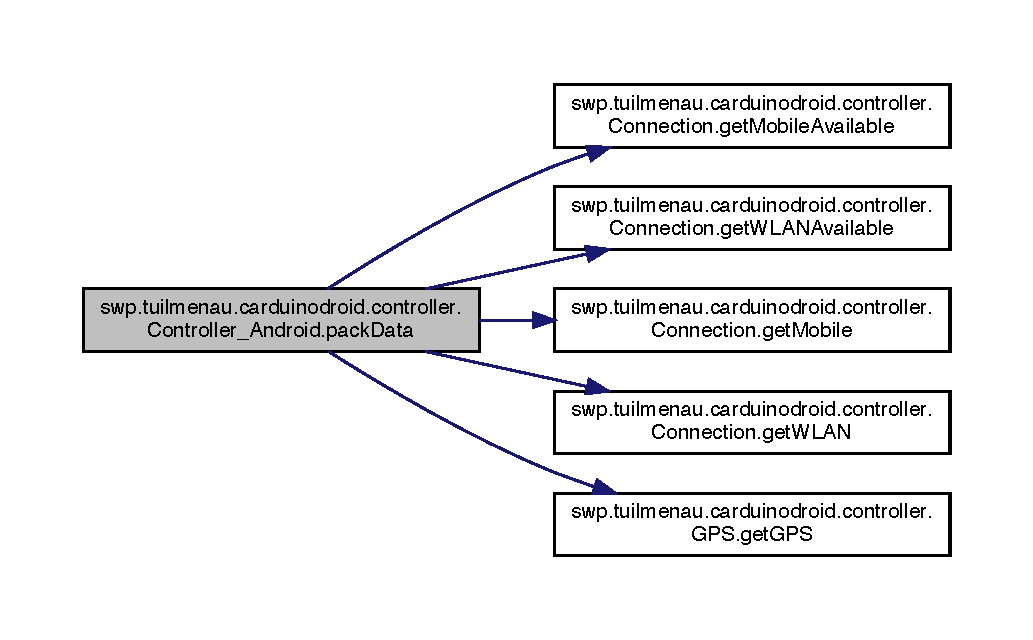
\includegraphics[width=350pt]{classswp_1_1tuilmenau_1_1carduinodroid_1_1controller_1_1_controller___android_ac8e21f14d9ed1c31500904a4f2a89242_cgraph}
\end{center}
\end{figure}




Here is the caller graph for this function\+:
\nopagebreak
\begin{figure}[H]
\begin{center}
\leavevmode
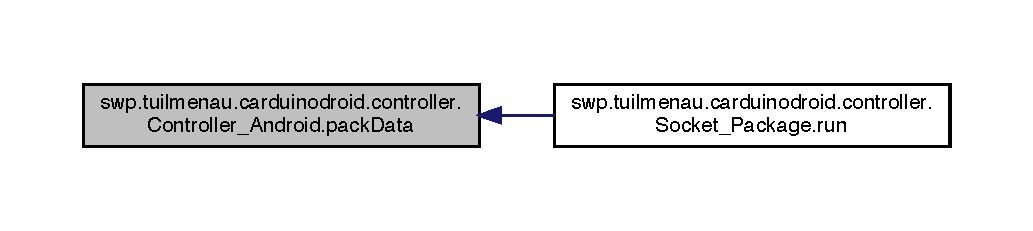
\includegraphics[width=350pt]{classswp_1_1tuilmenau_1_1carduinodroid_1_1controller_1_1_controller___android_ac8e21f14d9ed1c31500904a4f2a89242_icgraph}
\end{center}
\end{figure}


\hypertarget{classswp_1_1tuilmenau_1_1carduinodroid_1_1controller_1_1_controller___android_aee7580998e493c8fafa0ddd0dff31704}{}\index{swp\+::tuilmenau\+::carduinodroid\+::controller\+::\+Controller\+\_\+\+Android@{swp\+::tuilmenau\+::carduinodroid\+::controller\+::\+Controller\+\_\+\+Android}!receive\+Data@{receive\+Data}}
\index{receive\+Data@{receive\+Data}!swp\+::tuilmenau\+::carduinodroid\+::controller\+::\+Controller\+\_\+\+Android@{swp\+::tuilmenau\+::carduinodroid\+::controller\+::\+Controller\+\_\+\+Android}}
\subsubsection[{receive\+Data}]{\setlength{\rightskip}{0pt plus 5cm}void swp.\+tuilmenau.\+carduinodroid.\+controller.\+Controller\+\_\+\+Android.\+receive\+Data (
\begin{DoxyParamCaption}
\item[{String}]{data}
\end{DoxyParamCaption}
)}\label{classswp_1_1tuilmenau_1_1carduinodroid_1_1controller_1_1_controller___android_aee7580998e493c8fafa0ddd0dff31704}
Used to decode a packed command String received from the P\+C. After the decode the commands are executed.


\begin{DoxyParams}{Parameters}
{\em data} & A String containing the compressed Data as follows\+: 
\begin{DoxyEnumerate}
\item Control Signals with settings 
\item Camera Settings 
\begin{DoxyEnumerate}
\item Front or Back Camera 
\item Camera Resolution 
\item Camera Light 
\item Quality$<$/$>$ 
\end{DoxyEnumerate}
\item \hyperlink{classswp_1_1tuilmenau_1_1carduinodroid_1_1controller_1_1_sound}{Sound} Signals 
\begin{DoxyEnumerate}
\item Play a \hyperlink{classswp_1_1tuilmenau_1_1carduinodroid_1_1controller_1_1_sound}{Sound} by Android phone 
\item Start or Stop a Record 
\end{DoxyEnumerate}
\end{DoxyEnumerate}\\
\hline
\end{DoxyParams}


Here is the call graph for this function\+:
\nopagebreak
\begin{figure}[H]
\begin{center}
\leavevmode
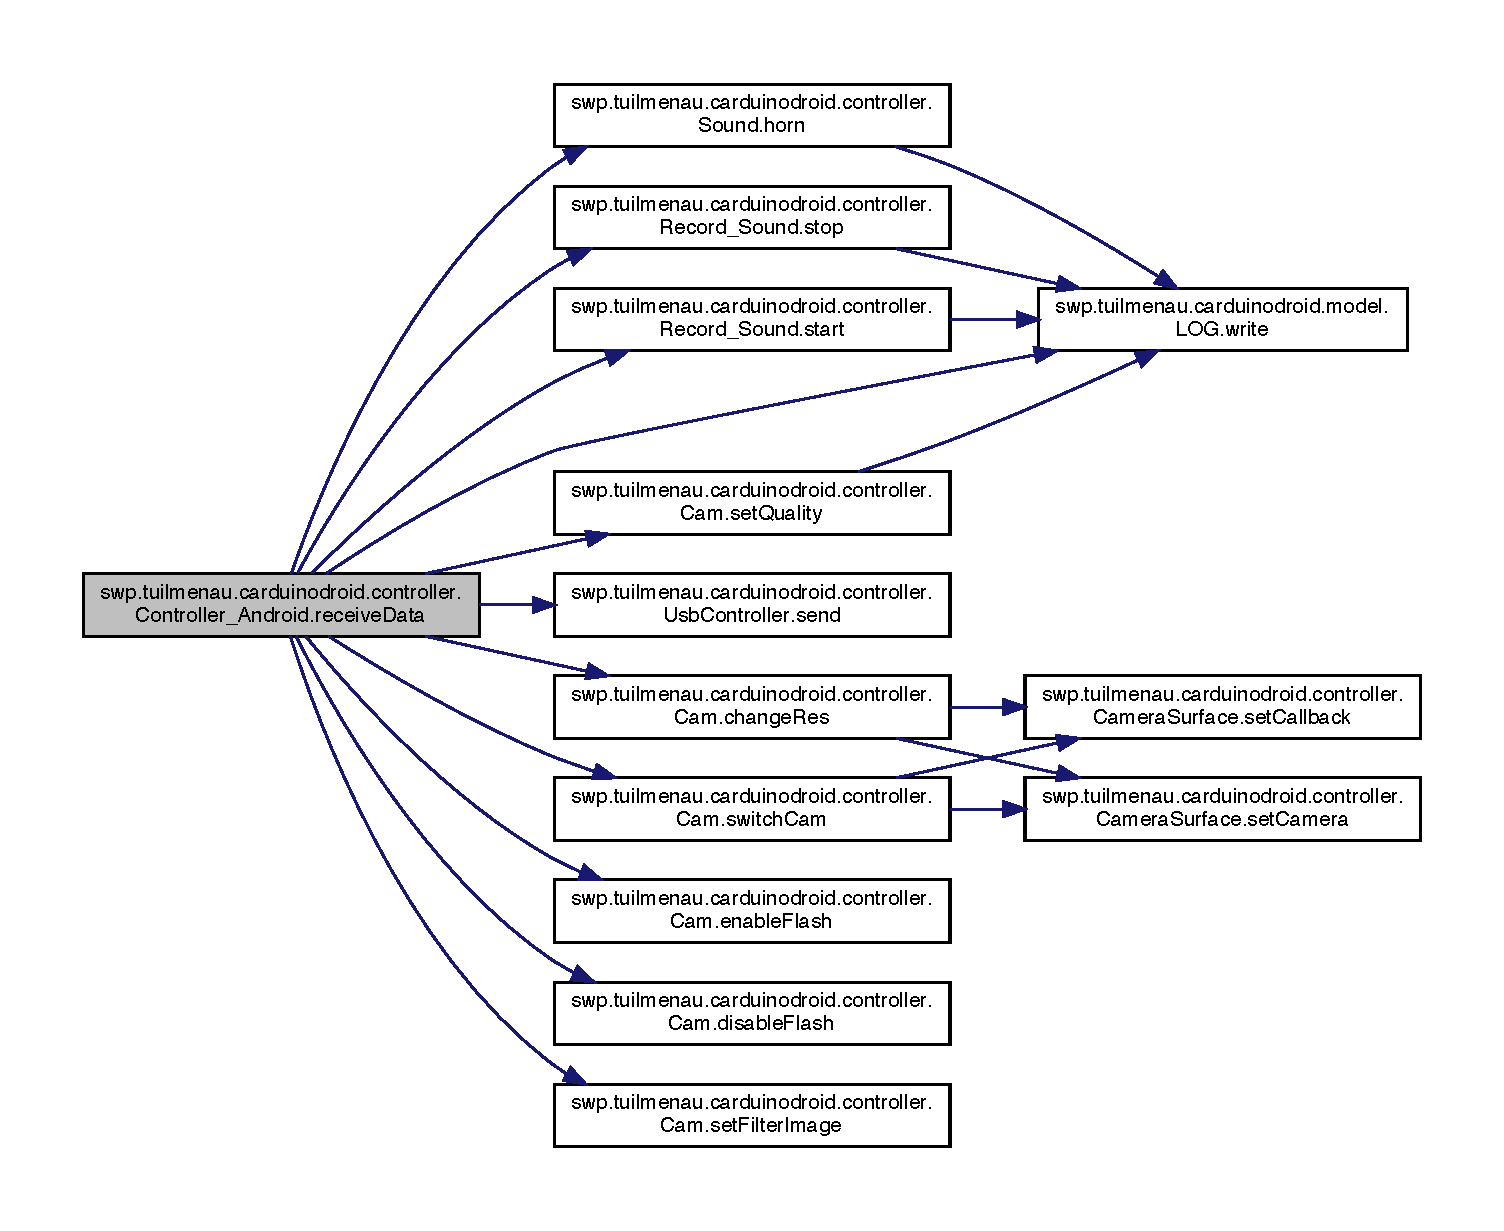
\includegraphics[width=350pt]{classswp_1_1tuilmenau_1_1carduinodroid_1_1controller_1_1_controller___android_aee7580998e493c8fafa0ddd0dff31704_cgraph}
\end{center}
\end{figure}




Here is the caller graph for this function\+:
\nopagebreak
\begin{figure}[H]
\begin{center}
\leavevmode
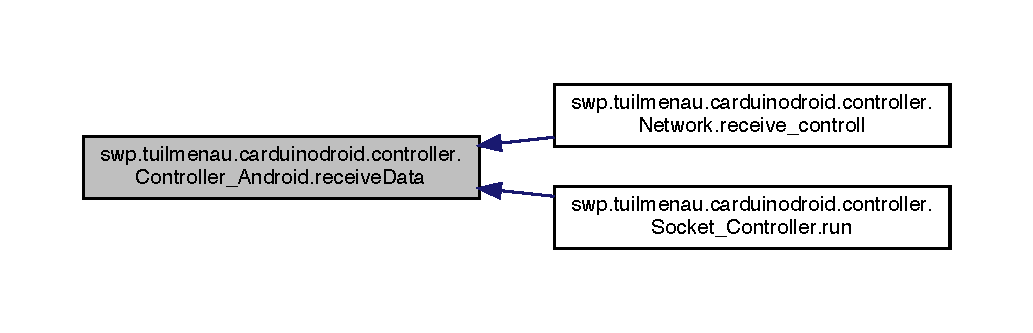
\includegraphics[width=350pt]{classswp_1_1tuilmenau_1_1carduinodroid_1_1controller_1_1_controller___android_aee7580998e493c8fafa0ddd0dff31704_icgraph}
\end{center}
\end{figure}


\hypertarget{classswp_1_1tuilmenau_1_1carduinodroid_1_1controller_1_1_controller___android_ae6de91d0d2653cfd019a473cfe8714a1}{}\index{swp\+::tuilmenau\+::carduinodroid\+::controller\+::\+Controller\+\_\+\+Android@{swp\+::tuilmenau\+::carduinodroid\+::controller\+::\+Controller\+\_\+\+Android}!set\+Network@{set\+Network}}
\index{set\+Network@{set\+Network}!swp\+::tuilmenau\+::carduinodroid\+::controller\+::\+Controller\+\_\+\+Android@{swp\+::tuilmenau\+::carduinodroid\+::controller\+::\+Controller\+\_\+\+Android}}
\subsubsection[{set\+Network}]{\setlength{\rightskip}{0pt plus 5cm}void swp.\+tuilmenau.\+carduinodroid.\+controller.\+Controller\+\_\+\+Android.\+set\+Network (
\begin{DoxyParamCaption}
\item[{{\bf Network}}]{network}
\end{DoxyParamCaption}
)}\label{classswp_1_1tuilmenau_1_1carduinodroid_1_1controller_1_1_controller___android_ae6de91d0d2653cfd019a473cfe8714a1}
Sets the \hyperlink{classswp_1_1tuilmenau_1_1carduinodroid_1_1controller_1_1_network}{Network}


\begin{DoxyParams}{Parameters}
{\em network} & the \hyperlink{classswp_1_1tuilmenau_1_1carduinodroid_1_1controller_1_1_network}{Network} to set. \\
\hline
\end{DoxyParams}


Here is the caller graph for this function\+:
\nopagebreak
\begin{figure}[H]
\begin{center}
\leavevmode
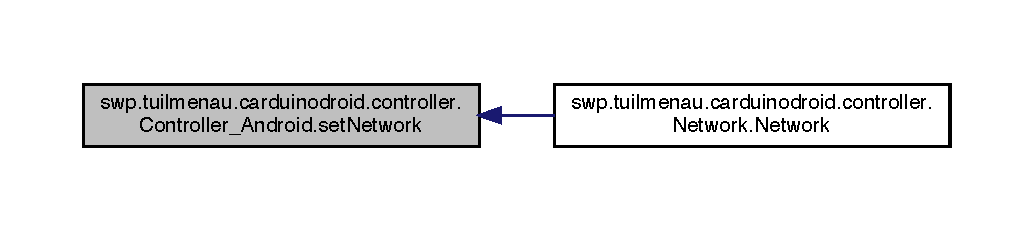
\includegraphics[width=350pt]{classswp_1_1tuilmenau_1_1carduinodroid_1_1controller_1_1_controller___android_ae6de91d0d2653cfd019a473cfe8714a1_icgraph}
\end{center}
\end{figure}


\hypertarget{classswp_1_1tuilmenau_1_1carduinodroid_1_1controller_1_1_controller___android_aa5f10c125c12e42da6b8eec6d922c7d1}{}\index{swp\+::tuilmenau\+::carduinodroid\+::controller\+::\+Controller\+\_\+\+Android@{swp\+::tuilmenau\+::carduinodroid\+::controller\+::\+Controller\+\_\+\+Android}!Set\+Sent@{Set\+Sent}}
\index{Set\+Sent@{Set\+Sent}!swp\+::tuilmenau\+::carduinodroid\+::controller\+::\+Controller\+\_\+\+Android@{swp\+::tuilmenau\+::carduinodroid\+::controller\+::\+Controller\+\_\+\+Android}}
\subsubsection[{Set\+Sent}]{\setlength{\rightskip}{0pt plus 5cm}void swp.\+tuilmenau.\+carduinodroid.\+controller.\+Controller\+\_\+\+Android.\+Set\+Sent (
\begin{DoxyParamCaption}
\item[{boolean}]{Sent}
\end{DoxyParamCaption}
)}\label{classswp_1_1tuilmenau_1_1carduinodroid_1_1controller_1_1_controller___android_aa5f10c125c12e42da6b8eec6d922c7d1}


\subsection{Member Data Documentation}
\hypertarget{classswp_1_1tuilmenau_1_1carduinodroid_1_1controller_1_1_controller___android_a759de099e5a0795e0450a6a2061cb50a}{}\index{swp\+::tuilmenau\+::carduinodroid\+::controller\+::\+Controller\+\_\+\+Android@{swp\+::tuilmenau\+::carduinodroid\+::controller\+::\+Controller\+\_\+\+Android}!A\+C\+T\+I\+V\+I\+T\+Y@{A\+C\+T\+I\+V\+I\+T\+Y}}
\index{A\+C\+T\+I\+V\+I\+T\+Y@{A\+C\+T\+I\+V\+I\+T\+Y}!swp\+::tuilmenau\+::carduinodroid\+::controller\+::\+Controller\+\_\+\+Android@{swp\+::tuilmenau\+::carduinodroid\+::controller\+::\+Controller\+\_\+\+Android}}
\subsubsection[{A\+C\+T\+I\+V\+I\+T\+Y}]{\setlength{\rightskip}{0pt plus 5cm}Activity swp.\+tuilmenau.\+carduinodroid.\+controller.\+Controller\+\_\+\+Android.\+A\+C\+T\+I\+V\+I\+T\+Y}\label{classswp_1_1tuilmenau_1_1carduinodroid_1_1controller_1_1_controller___android_a759de099e5a0795e0450a6a2061cb50a}
\hypertarget{classswp_1_1tuilmenau_1_1carduinodroid_1_1controller_1_1_controller___android_a31da0a49fe10962abd4aa0322e9f30d0}{}\index{swp\+::tuilmenau\+::carduinodroid\+::controller\+::\+Controller\+\_\+\+Android@{swp\+::tuilmenau\+::carduinodroid\+::controller\+::\+Controller\+\_\+\+Android}!cam@{cam}}
\index{cam@{cam}!swp\+::tuilmenau\+::carduinodroid\+::controller\+::\+Controller\+\_\+\+Android@{swp\+::tuilmenau\+::carduinodroid\+::controller\+::\+Controller\+\_\+\+Android}}
\subsubsection[{cam}]{\setlength{\rightskip}{0pt plus 5cm}{\bf Cam} swp.\+tuilmenau.\+carduinodroid.\+controller.\+Controller\+\_\+\+Android.\+cam}\label{classswp_1_1tuilmenau_1_1carduinodroid_1_1controller_1_1_controller___android_a31da0a49fe10962abd4aa0322e9f30d0}
\hypertarget{classswp_1_1tuilmenau_1_1carduinodroid_1_1controller_1_1_controller___android_a3058848b90ad1bda3b7d9d873e28ac42}{}\index{swp\+::tuilmenau\+::carduinodroid\+::controller\+::\+Controller\+\_\+\+Android@{swp\+::tuilmenau\+::carduinodroid\+::controller\+::\+Controller\+\_\+\+Android}!connection@{connection}}
\index{connection@{connection}!swp\+::tuilmenau\+::carduinodroid\+::controller\+::\+Controller\+\_\+\+Android@{swp\+::tuilmenau\+::carduinodroid\+::controller\+::\+Controller\+\_\+\+Android}}
\subsubsection[{connection}]{\setlength{\rightskip}{0pt plus 5cm}{\bf Connection} swp.\+tuilmenau.\+carduinodroid.\+controller.\+Controller\+\_\+\+Android.\+connection}\label{classswp_1_1tuilmenau_1_1carduinodroid_1_1controller_1_1_controller___android_a3058848b90ad1bda3b7d9d873e28ac42}
\hypertarget{classswp_1_1tuilmenau_1_1carduinodroid_1_1controller_1_1_controller___android_ad9f00966717e095bf966440a3d3f2df0}{}\index{swp\+::tuilmenau\+::carduinodroid\+::controller\+::\+Controller\+\_\+\+Android@{swp\+::tuilmenau\+::carduinodroid\+::controller\+::\+Controller\+\_\+\+Android}!gps@{gps}}
\index{gps@{gps}!swp\+::tuilmenau\+::carduinodroid\+::controller\+::\+Controller\+\_\+\+Android@{swp\+::tuilmenau\+::carduinodroid\+::controller\+::\+Controller\+\_\+\+Android}}
\subsubsection[{gps}]{\setlength{\rightskip}{0pt plus 5cm}{\bf G\+P\+S} swp.\+tuilmenau.\+carduinodroid.\+controller.\+Controller\+\_\+\+Android.\+gps}\label{classswp_1_1tuilmenau_1_1carduinodroid_1_1controller_1_1_controller___android_ad9f00966717e095bf966440a3d3f2df0}
\hypertarget{classswp_1_1tuilmenau_1_1carduinodroid_1_1controller_1_1_controller___android_affcd564aa1e60c3f85bc6a28864c1d34}{}\index{swp\+::tuilmenau\+::carduinodroid\+::controller\+::\+Controller\+\_\+\+Android@{swp\+::tuilmenau\+::carduinodroid\+::controller\+::\+Controller\+\_\+\+Android}!log@{log}}
\index{log@{log}!swp\+::tuilmenau\+::carduinodroid\+::controller\+::\+Controller\+\_\+\+Android@{swp\+::tuilmenau\+::carduinodroid\+::controller\+::\+Controller\+\_\+\+Android}}
\subsubsection[{log}]{\setlength{\rightskip}{0pt plus 5cm}{\bf L\+O\+G} swp.\+tuilmenau.\+carduinodroid.\+controller.\+Controller\+\_\+\+Android.\+log}\label{classswp_1_1tuilmenau_1_1carduinodroid_1_1controller_1_1_controller___android_affcd564aa1e60c3f85bc6a28864c1d34}
\hypertarget{classswp_1_1tuilmenau_1_1carduinodroid_1_1controller_1_1_controller___android_af9cb0b01ab817f064e722a70b0a07987}{}\index{swp\+::tuilmenau\+::carduinodroid\+::controller\+::\+Controller\+\_\+\+Android@{swp\+::tuilmenau\+::carduinodroid\+::controller\+::\+Controller\+\_\+\+Android}!network@{network}}
\index{network@{network}!swp\+::tuilmenau\+::carduinodroid\+::controller\+::\+Controller\+\_\+\+Android@{swp\+::tuilmenau\+::carduinodroid\+::controller\+::\+Controller\+\_\+\+Android}}
\subsubsection[{network}]{\setlength{\rightskip}{0pt plus 5cm}{\bf Network} swp.\+tuilmenau.\+carduinodroid.\+controller.\+Controller\+\_\+\+Android.\+network}\label{classswp_1_1tuilmenau_1_1carduinodroid_1_1controller_1_1_controller___android_af9cb0b01ab817f064e722a70b0a07987}
\hypertarget{classswp_1_1tuilmenau_1_1carduinodroid_1_1controller_1_1_controller___android_a72ea9edd25ca9ef34e5cc7d0facbcd28}{}\index{swp\+::tuilmenau\+::carduinodroid\+::controller\+::\+Controller\+\_\+\+Android@{swp\+::tuilmenau\+::carduinodroid\+::controller\+::\+Controller\+\_\+\+Android}!record\+\_\+sound@{record\+\_\+sound}}
\index{record\+\_\+sound@{record\+\_\+sound}!swp\+::tuilmenau\+::carduinodroid\+::controller\+::\+Controller\+\_\+\+Android@{swp\+::tuilmenau\+::carduinodroid\+::controller\+::\+Controller\+\_\+\+Android}}
\subsubsection[{record\+\_\+sound}]{\setlength{\rightskip}{0pt plus 5cm}{\bf Record\+\_\+\+Sound} swp.\+tuilmenau.\+carduinodroid.\+controller.\+Controller\+\_\+\+Android.\+record\+\_\+sound}\label{classswp_1_1tuilmenau_1_1carduinodroid_1_1controller_1_1_controller___android_a72ea9edd25ca9ef34e5cc7d0facbcd28}
\hypertarget{classswp_1_1tuilmenau_1_1carduinodroid_1_1controller_1_1_controller___android_a45238bf1102e9589bc83c439e6e28b8e}{}\index{swp\+::tuilmenau\+::carduinodroid\+::controller\+::\+Controller\+\_\+\+Android@{swp\+::tuilmenau\+::carduinodroid\+::controller\+::\+Controller\+\_\+\+Android}!sent@{sent}}
\index{sent@{sent}!swp\+::tuilmenau\+::carduinodroid\+::controller\+::\+Controller\+\_\+\+Android@{swp\+::tuilmenau\+::carduinodroid\+::controller\+::\+Controller\+\_\+\+Android}}
\subsubsection[{sent}]{\setlength{\rightskip}{0pt plus 5cm}boolean swp.\+tuilmenau.\+carduinodroid.\+controller.\+Controller\+\_\+\+Android.\+sent}\label{classswp_1_1tuilmenau_1_1carduinodroid_1_1controller_1_1_controller___android_a45238bf1102e9589bc83c439e6e28b8e}
\hypertarget{classswp_1_1tuilmenau_1_1carduinodroid_1_1controller_1_1_controller___android_a72efe09e3412212d419018ef46080580}{}\index{swp\+::tuilmenau\+::carduinodroid\+::controller\+::\+Controller\+\_\+\+Android@{swp\+::tuilmenau\+::carduinodroid\+::controller\+::\+Controller\+\_\+\+Android}!sentfree@{sentfree}}
\index{sentfree@{sentfree}!swp\+::tuilmenau\+::carduinodroid\+::controller\+::\+Controller\+\_\+\+Android@{swp\+::tuilmenau\+::carduinodroid\+::controller\+::\+Controller\+\_\+\+Android}}
\subsubsection[{sentfree}]{\setlength{\rightskip}{0pt plus 5cm}boolean swp.\+tuilmenau.\+carduinodroid.\+controller.\+Controller\+\_\+\+Android.\+sentfree}\label{classswp_1_1tuilmenau_1_1carduinodroid_1_1controller_1_1_controller___android_a72efe09e3412212d419018ef46080580}
\hypertarget{classswp_1_1tuilmenau_1_1carduinodroid_1_1controller_1_1_controller___android_af52db04dd80233d572b0fd66e1cf224f}{}\index{swp\+::tuilmenau\+::carduinodroid\+::controller\+::\+Controller\+\_\+\+Android@{swp\+::tuilmenau\+::carduinodroid\+::controller\+::\+Controller\+\_\+\+Android}!sound@{sound}}
\index{sound@{sound}!swp\+::tuilmenau\+::carduinodroid\+::controller\+::\+Controller\+\_\+\+Android@{swp\+::tuilmenau\+::carduinodroid\+::controller\+::\+Controller\+\_\+\+Android}}
\subsubsection[{sound}]{\setlength{\rightskip}{0pt plus 5cm}{\bf Sound} swp.\+tuilmenau.\+carduinodroid.\+controller.\+Controller\+\_\+\+Android.\+sound}\label{classswp_1_1tuilmenau_1_1carduinodroid_1_1controller_1_1_controller___android_af52db04dd80233d572b0fd66e1cf224f}


The documentation for this class was generated from the following file\+:\begin{DoxyCompactItemize}
\item 
src/swp/tuilmenau/carduinodroid/controller/\hyperlink{_controller___android_8java}{Controller\+\_\+\+Android.\+java}\end{DoxyCompactItemize}

\hypertarget{classswp_1_1tuilmenau_1_1carduinodroid_1_1_filter_1_1_filter_factory}{}\section{swp.\+tuilmenau.\+carduinodroid.\+Filter.\+Filter\+Factory Class Reference}
\label{classswp_1_1tuilmenau_1_1carduinodroid_1_1_filter_1_1_filter_factory}\index{swp.\+tuilmenau.\+carduinodroid.\+Filter.\+Filter\+Factory@{swp.\+tuilmenau.\+carduinodroid.\+Filter.\+Filter\+Factory}}


Collaboration diagram for swp.\+tuilmenau.\+carduinodroid.\+Filter.\+Filter\+Factory\+:
\nopagebreak
\begin{figure}[H]
\begin{center}
\leavevmode
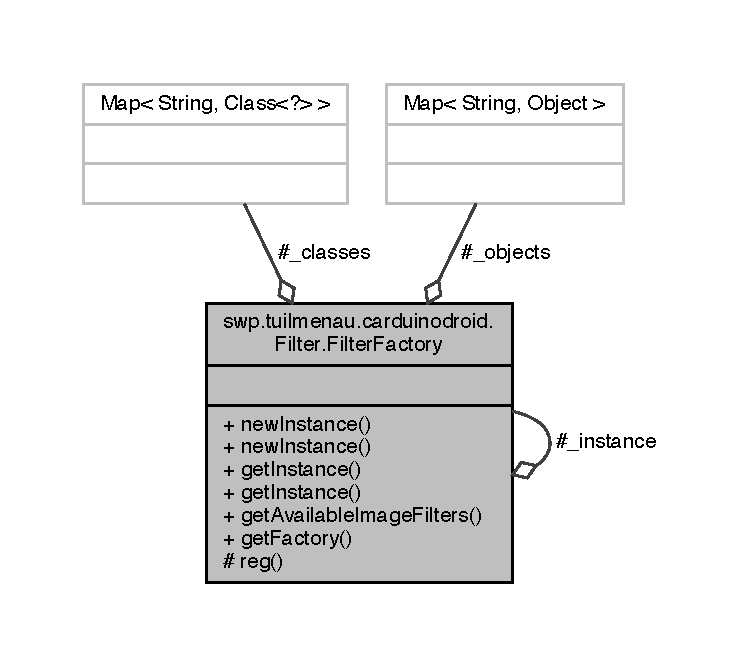
\includegraphics[width=350pt]{classswp_1_1tuilmenau_1_1carduinodroid_1_1_filter_1_1_filter_factory__coll__graph}
\end{center}
\end{figure}
\subsection*{Public Member Functions}
\begin{DoxyCompactItemize}
\item 
\hyperlink{classswp_1_1tuilmenau_1_1carduinodroid_1_1_filter_1_1_image_filter}{Image\+Filter} \hyperlink{classswp_1_1tuilmenau_1_1carduinodroid_1_1_filter_1_1_filter_factory_aff05b810c3776ef74643da75f46a2ceb}{new\+Instance} (String filter\+Type, Class$<$?$>$\mbox{[}$\,$\mbox{]} param\+Types, Object\mbox{[}$\,$\mbox{]} params)
\item 
\hyperlink{classswp_1_1tuilmenau_1_1carduinodroid_1_1_filter_1_1_image_filter}{Image\+Filter} \hyperlink{classswp_1_1tuilmenau_1_1carduinodroid_1_1_filter_1_1_filter_factory_a03f77013bf07ec12a141c947816072e5}{new\+Instance} (String filter\+Type)
\item 
\hyperlink{classswp_1_1tuilmenau_1_1carduinodroid_1_1_filter_1_1_image_filter}{Image\+Filter} \hyperlink{classswp_1_1tuilmenau_1_1carduinodroid_1_1_filter_1_1_filter_factory_aaabe4677d10eb29acd7efa33448d890d}{get\+Instance} (String filter\+Type, Class$<$?$>$\mbox{[}$\,$\mbox{]} param\+Types, Object\mbox{[}$\,$\mbox{]} params)
\item 
\hyperlink{classswp_1_1tuilmenau_1_1carduinodroid_1_1_filter_1_1_image_filter}{Image\+Filter} \hyperlink{classswp_1_1tuilmenau_1_1carduinodroid_1_1_filter_1_1_filter_factory_a7fa87ecc5317ef686e0fcbc995c4390d}{get\+Instance} (String filter\+Type)
\item 
Set$<$ String $>$ \hyperlink{classswp_1_1tuilmenau_1_1carduinodroid_1_1_filter_1_1_filter_factory_aa0f244ab827c355cd7fc4a7eb7f95096}{get\+Available\+Image\+Filters} ()
\end{DoxyCompactItemize}
\subsection*{Static Public Member Functions}
\begin{DoxyCompactItemize}
\item 
static \hyperlink{classswp_1_1tuilmenau_1_1carduinodroid_1_1_filter_1_1_filter_factory}{Filter\+Factory} \hyperlink{classswp_1_1tuilmenau_1_1carduinodroid_1_1_filter_1_1_filter_factory_af9d1456b900a8d8f2874ef8d7dfbd702}{get\+Factory} ()
\end{DoxyCompactItemize}
\subsection*{Protected Member Functions}
\begin{DoxyCompactItemize}
\item 
void \hyperlink{classswp_1_1tuilmenau_1_1carduinodroid_1_1_filter_1_1_filter_factory_a3d602fb6f6b280e7135e1fa41aaa6a29}{reg} (String filter\+Type, Class$<$?$>$ clazz)
\end{DoxyCompactItemize}
\subsection*{Protected Attributes}
\begin{DoxyCompactItemize}
\item 
Map$<$ String, Object $>$ \hyperlink{classswp_1_1tuilmenau_1_1carduinodroid_1_1_filter_1_1_filter_factory_a8015fffcdd394fc33a983953771bb875}{\+\_\+objects} = new Tree\+Map$<$String, Object$>$()
\end{DoxyCompactItemize}
\subsection*{Static Protected Attributes}
\begin{DoxyCompactItemize}
\item 
static Map$<$ String, Class$<$?$>$ $>$ \hyperlink{classswp_1_1tuilmenau_1_1carduinodroid_1_1_filter_1_1_filter_factory_ab0d48ea8b973fc9a97a480d6d7942c02}{\+\_\+classes} = new Tree\+Map$<$String, Class$<$?$>$$>$()
\item 
static \hyperlink{classswp_1_1tuilmenau_1_1carduinodroid_1_1_filter_1_1_filter_factory}{Filter\+Factory} \hyperlink{classswp_1_1tuilmenau_1_1carduinodroid_1_1_filter_1_1_filter_factory_ace6d6288eefdca08fc97e0aeab5409a0}{\+\_\+instance}
\end{DoxyCompactItemize}


\subsection{Member Function Documentation}
\hypertarget{classswp_1_1tuilmenau_1_1carduinodroid_1_1_filter_1_1_filter_factory_aa0f244ab827c355cd7fc4a7eb7f95096}{}\index{swp\+::tuilmenau\+::carduinodroid\+::\+Filter\+::\+Filter\+Factory@{swp\+::tuilmenau\+::carduinodroid\+::\+Filter\+::\+Filter\+Factory}!get\+Available\+Image\+Filters@{get\+Available\+Image\+Filters}}
\index{get\+Available\+Image\+Filters@{get\+Available\+Image\+Filters}!swp\+::tuilmenau\+::carduinodroid\+::\+Filter\+::\+Filter\+Factory@{swp\+::tuilmenau\+::carduinodroid\+::\+Filter\+::\+Filter\+Factory}}
\subsubsection[{get\+Available\+Image\+Filters}]{\setlength{\rightskip}{0pt plus 5cm}Set$<$String$>$ swp.\+tuilmenau.\+carduinodroid.\+Filter.\+Filter\+Factory.\+get\+Available\+Image\+Filters (
\begin{DoxyParamCaption}
{}
\end{DoxyParamCaption}
)}\label{classswp_1_1tuilmenau_1_1carduinodroid_1_1_filter_1_1_filter_factory_aa0f244ab827c355cd7fc4a7eb7f95096}


Here is the caller graph for this function\+:
\nopagebreak
\begin{figure}[H]
\begin{center}
\leavevmode
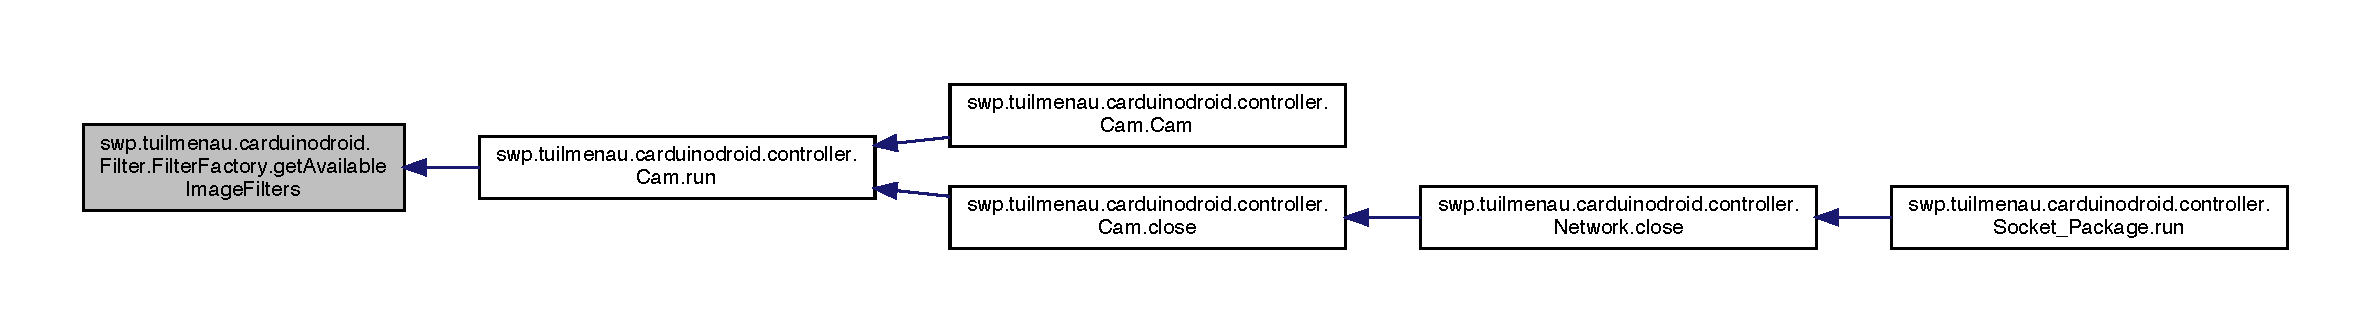
\includegraphics[width=350pt]{classswp_1_1tuilmenau_1_1carduinodroid_1_1_filter_1_1_filter_factory_aa0f244ab827c355cd7fc4a7eb7f95096_icgraph}
\end{center}
\end{figure}


\hypertarget{classswp_1_1tuilmenau_1_1carduinodroid_1_1_filter_1_1_filter_factory_af9d1456b900a8d8f2874ef8d7dfbd702}{}\index{swp\+::tuilmenau\+::carduinodroid\+::\+Filter\+::\+Filter\+Factory@{swp\+::tuilmenau\+::carduinodroid\+::\+Filter\+::\+Filter\+Factory}!get\+Factory@{get\+Factory}}
\index{get\+Factory@{get\+Factory}!swp\+::tuilmenau\+::carduinodroid\+::\+Filter\+::\+Filter\+Factory@{swp\+::tuilmenau\+::carduinodroid\+::\+Filter\+::\+Filter\+Factory}}
\subsubsection[{get\+Factory}]{\setlength{\rightskip}{0pt plus 5cm}static {\bf Filter\+Factory} swp.\+tuilmenau.\+carduinodroid.\+Filter.\+Filter\+Factory.\+get\+Factory (
\begin{DoxyParamCaption}
{}
\end{DoxyParamCaption}
)\hspace{0.3cm}{\ttfamily [static]}}\label{classswp_1_1tuilmenau_1_1carduinodroid_1_1_filter_1_1_filter_factory_af9d1456b900a8d8f2874ef8d7dfbd702}


Here is the caller graph for this function\+:
\nopagebreak
\begin{figure}[H]
\begin{center}
\leavevmode
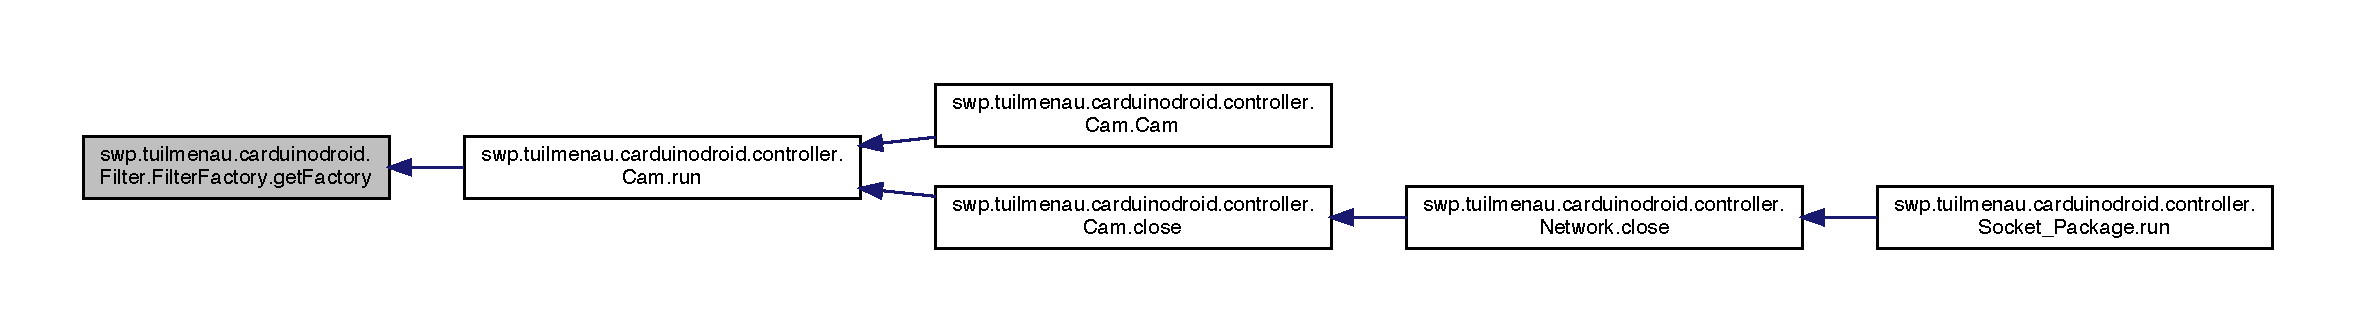
\includegraphics[width=350pt]{classswp_1_1tuilmenau_1_1carduinodroid_1_1_filter_1_1_filter_factory_af9d1456b900a8d8f2874ef8d7dfbd702_icgraph}
\end{center}
\end{figure}


\hypertarget{classswp_1_1tuilmenau_1_1carduinodroid_1_1_filter_1_1_filter_factory_aaabe4677d10eb29acd7efa33448d890d}{}\index{swp\+::tuilmenau\+::carduinodroid\+::\+Filter\+::\+Filter\+Factory@{swp\+::tuilmenau\+::carduinodroid\+::\+Filter\+::\+Filter\+Factory}!get\+Instance@{get\+Instance}}
\index{get\+Instance@{get\+Instance}!swp\+::tuilmenau\+::carduinodroid\+::\+Filter\+::\+Filter\+Factory@{swp\+::tuilmenau\+::carduinodroid\+::\+Filter\+::\+Filter\+Factory}}
\subsubsection[{get\+Instance}]{\setlength{\rightskip}{0pt plus 5cm}{\bf Image\+Filter} swp.\+tuilmenau.\+carduinodroid.\+Filter.\+Filter\+Factory.\+get\+Instance (
\begin{DoxyParamCaption}
\item[{String}]{filter\+Type, }
\item[{Class$<$?$>$\mbox{[}$\,$\mbox{]}}]{param\+Types, }
\item[{Object\mbox{[}$\,$\mbox{]}}]{params}
\end{DoxyParamCaption}
)}\label{classswp_1_1tuilmenau_1_1carduinodroid_1_1_filter_1_1_filter_factory_aaabe4677d10eb29acd7efa33448d890d}
Returns a singleton instance of the class 

Here is the call graph for this function\+:
\nopagebreak
\begin{figure}[H]
\begin{center}
\leavevmode
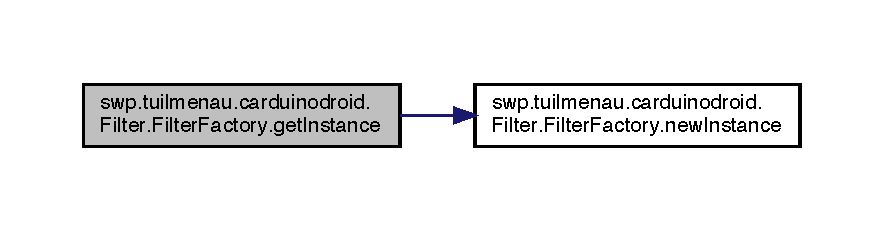
\includegraphics[width=350pt]{classswp_1_1tuilmenau_1_1carduinodroid_1_1_filter_1_1_filter_factory_aaabe4677d10eb29acd7efa33448d890d_cgraph}
\end{center}
\end{figure}




Here is the caller graph for this function\+:
\nopagebreak
\begin{figure}[H]
\begin{center}
\leavevmode
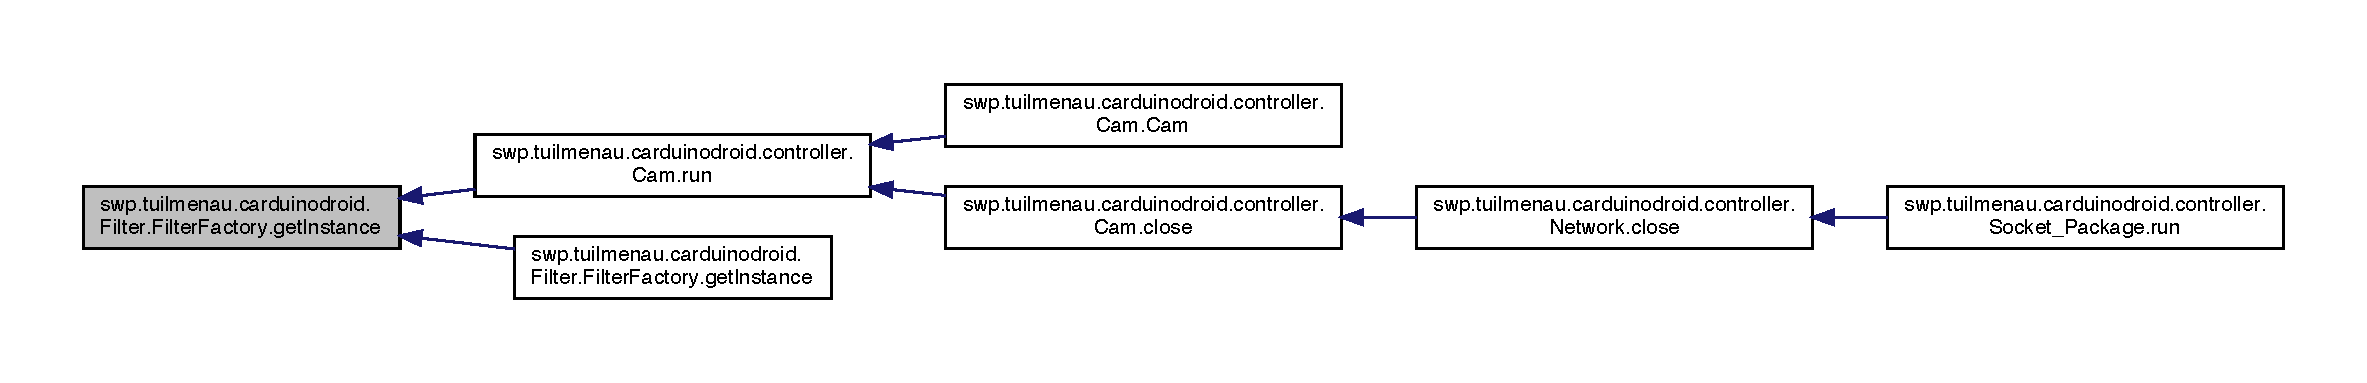
\includegraphics[width=350pt]{classswp_1_1tuilmenau_1_1carduinodroid_1_1_filter_1_1_filter_factory_aaabe4677d10eb29acd7efa33448d890d_icgraph}
\end{center}
\end{figure}


\hypertarget{classswp_1_1tuilmenau_1_1carduinodroid_1_1_filter_1_1_filter_factory_a7fa87ecc5317ef686e0fcbc995c4390d}{}\index{swp\+::tuilmenau\+::carduinodroid\+::\+Filter\+::\+Filter\+Factory@{swp\+::tuilmenau\+::carduinodroid\+::\+Filter\+::\+Filter\+Factory}!get\+Instance@{get\+Instance}}
\index{get\+Instance@{get\+Instance}!swp\+::tuilmenau\+::carduinodroid\+::\+Filter\+::\+Filter\+Factory@{swp\+::tuilmenau\+::carduinodroid\+::\+Filter\+::\+Filter\+Factory}}
\subsubsection[{get\+Instance}]{\setlength{\rightskip}{0pt plus 5cm}{\bf Image\+Filter} swp.\+tuilmenau.\+carduinodroid.\+Filter.\+Filter\+Factory.\+get\+Instance (
\begin{DoxyParamCaption}
\item[{String}]{filter\+Type}
\end{DoxyParamCaption}
)}\label{classswp_1_1tuilmenau_1_1carduinodroid_1_1_filter_1_1_filter_factory_a7fa87ecc5317ef686e0fcbc995c4390d}


Here is the call graph for this function\+:
\nopagebreak
\begin{figure}[H]
\begin{center}
\leavevmode
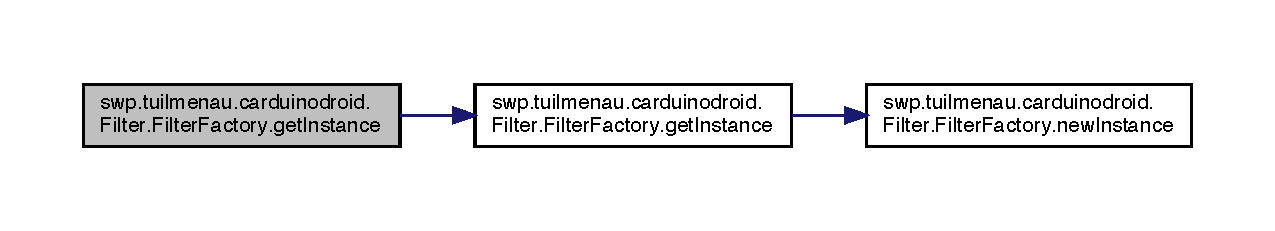
\includegraphics[width=350pt]{classswp_1_1tuilmenau_1_1carduinodroid_1_1_filter_1_1_filter_factory_a7fa87ecc5317ef686e0fcbc995c4390d_cgraph}
\end{center}
\end{figure}


\hypertarget{classswp_1_1tuilmenau_1_1carduinodroid_1_1_filter_1_1_filter_factory_aff05b810c3776ef74643da75f46a2ceb}{}\index{swp\+::tuilmenau\+::carduinodroid\+::\+Filter\+::\+Filter\+Factory@{swp\+::tuilmenau\+::carduinodroid\+::\+Filter\+::\+Filter\+Factory}!new\+Instance@{new\+Instance}}
\index{new\+Instance@{new\+Instance}!swp\+::tuilmenau\+::carduinodroid\+::\+Filter\+::\+Filter\+Factory@{swp\+::tuilmenau\+::carduinodroid\+::\+Filter\+::\+Filter\+Factory}}
\subsubsection[{new\+Instance}]{\setlength{\rightskip}{0pt plus 5cm}{\bf Image\+Filter} swp.\+tuilmenau.\+carduinodroid.\+Filter.\+Filter\+Factory.\+new\+Instance (
\begin{DoxyParamCaption}
\item[{String}]{filter\+Type, }
\item[{Class$<$?$>$\mbox{[}$\,$\mbox{]}}]{param\+Types, }
\item[{Object\mbox{[}$\,$\mbox{]}}]{params}
\end{DoxyParamCaption}
)}\label{classswp_1_1tuilmenau_1_1carduinodroid_1_1_filter_1_1_filter_factory_aff05b810c3776ef74643da75f46a2ceb}


Here is the caller graph for this function\+:
\nopagebreak
\begin{figure}[H]
\begin{center}
\leavevmode
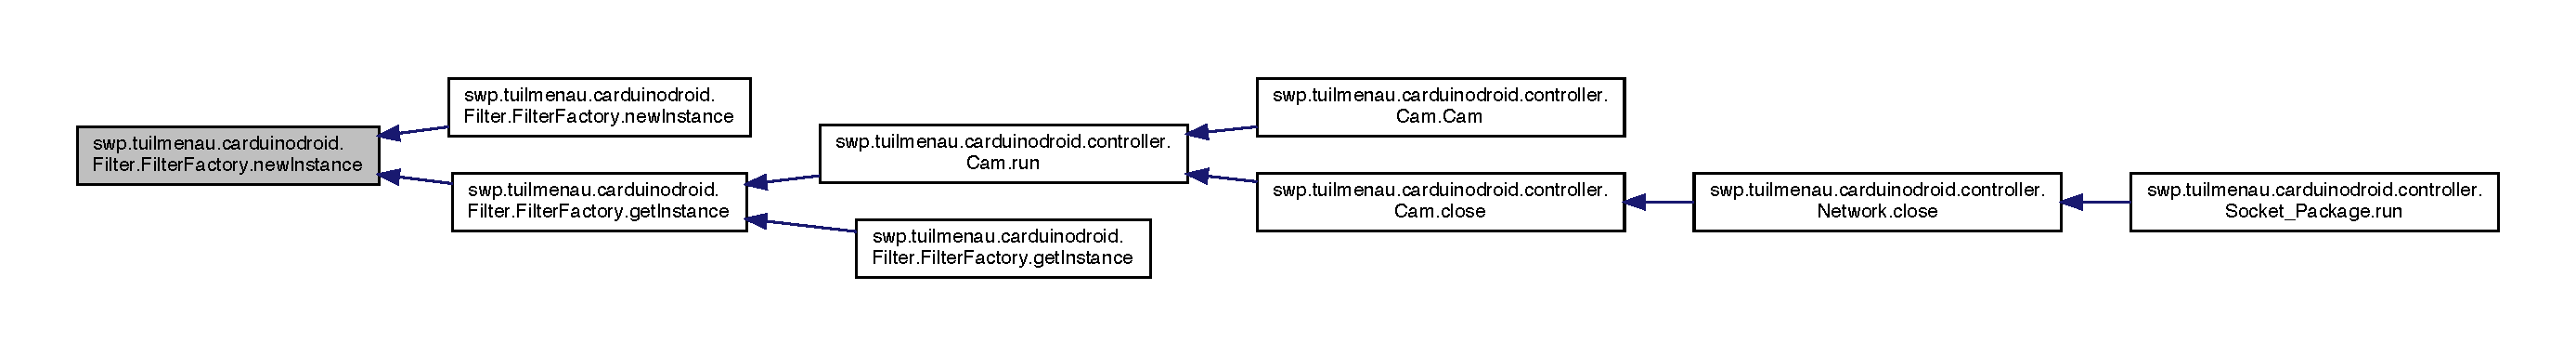
\includegraphics[width=350pt]{classswp_1_1tuilmenau_1_1carduinodroid_1_1_filter_1_1_filter_factory_aff05b810c3776ef74643da75f46a2ceb_icgraph}
\end{center}
\end{figure}


\hypertarget{classswp_1_1tuilmenau_1_1carduinodroid_1_1_filter_1_1_filter_factory_a03f77013bf07ec12a141c947816072e5}{}\index{swp\+::tuilmenau\+::carduinodroid\+::\+Filter\+::\+Filter\+Factory@{swp\+::tuilmenau\+::carduinodroid\+::\+Filter\+::\+Filter\+Factory}!new\+Instance@{new\+Instance}}
\index{new\+Instance@{new\+Instance}!swp\+::tuilmenau\+::carduinodroid\+::\+Filter\+::\+Filter\+Factory@{swp\+::tuilmenau\+::carduinodroid\+::\+Filter\+::\+Filter\+Factory}}
\subsubsection[{new\+Instance}]{\setlength{\rightskip}{0pt plus 5cm}{\bf Image\+Filter} swp.\+tuilmenau.\+carduinodroid.\+Filter.\+Filter\+Factory.\+new\+Instance (
\begin{DoxyParamCaption}
\item[{String}]{filter\+Type}
\end{DoxyParamCaption}
)}\label{classswp_1_1tuilmenau_1_1carduinodroid_1_1_filter_1_1_filter_factory_a03f77013bf07ec12a141c947816072e5}


Here is the call graph for this function\+:
\nopagebreak
\begin{figure}[H]
\begin{center}
\leavevmode
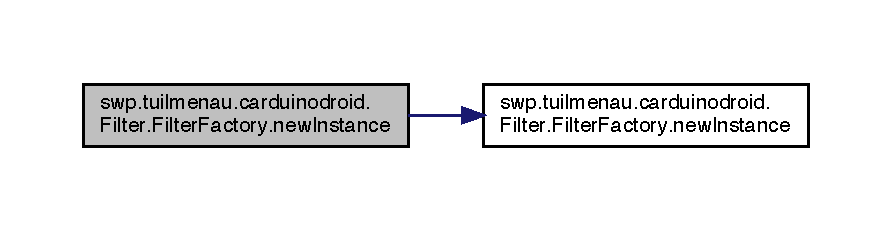
\includegraphics[width=350pt]{classswp_1_1tuilmenau_1_1carduinodroid_1_1_filter_1_1_filter_factory_a03f77013bf07ec12a141c947816072e5_cgraph}
\end{center}
\end{figure}


\hypertarget{classswp_1_1tuilmenau_1_1carduinodroid_1_1_filter_1_1_filter_factory_a3d602fb6f6b280e7135e1fa41aaa6a29}{}\index{swp\+::tuilmenau\+::carduinodroid\+::\+Filter\+::\+Filter\+Factory@{swp\+::tuilmenau\+::carduinodroid\+::\+Filter\+::\+Filter\+Factory}!reg@{reg}}
\index{reg@{reg}!swp\+::tuilmenau\+::carduinodroid\+::\+Filter\+::\+Filter\+Factory@{swp\+::tuilmenau\+::carduinodroid\+::\+Filter\+::\+Filter\+Factory}}
\subsubsection[{reg}]{\setlength{\rightskip}{0pt plus 5cm}void swp.\+tuilmenau.\+carduinodroid.\+Filter.\+Filter\+Factory.\+reg (
\begin{DoxyParamCaption}
\item[{String}]{filter\+Type, }
\item[{Class$<$?$>$}]{clazz}
\end{DoxyParamCaption}
)\hspace{0.3cm}{\ttfamily [protected]}}\label{classswp_1_1tuilmenau_1_1carduinodroid_1_1_filter_1_1_filter_factory_a3d602fb6f6b280e7135e1fa41aaa6a29}


\subsection{Member Data Documentation}
\hypertarget{classswp_1_1tuilmenau_1_1carduinodroid_1_1_filter_1_1_filter_factory_ab0d48ea8b973fc9a97a480d6d7942c02}{}\index{swp\+::tuilmenau\+::carduinodroid\+::\+Filter\+::\+Filter\+Factory@{swp\+::tuilmenau\+::carduinodroid\+::\+Filter\+::\+Filter\+Factory}!\+\_\+classes@{\+\_\+classes}}
\index{\+\_\+classes@{\+\_\+classes}!swp\+::tuilmenau\+::carduinodroid\+::\+Filter\+::\+Filter\+Factory@{swp\+::tuilmenau\+::carduinodroid\+::\+Filter\+::\+Filter\+Factory}}
\subsubsection[{\+\_\+classes}]{\setlength{\rightskip}{0pt plus 5cm}Map$<$String, Class$<$?$>$ $>$ swp.\+tuilmenau.\+carduinodroid.\+Filter.\+Filter\+Factory.\+\_\+classes = new Tree\+Map$<$String, Class$<$?$>$$>$()\hspace{0.3cm}{\ttfamily [static]}, {\ttfamily [protected]}}\label{classswp_1_1tuilmenau_1_1carduinodroid_1_1_filter_1_1_filter_factory_ab0d48ea8b973fc9a97a480d6d7942c02}
\hypertarget{classswp_1_1tuilmenau_1_1carduinodroid_1_1_filter_1_1_filter_factory_ace6d6288eefdca08fc97e0aeab5409a0}{}\index{swp\+::tuilmenau\+::carduinodroid\+::\+Filter\+::\+Filter\+Factory@{swp\+::tuilmenau\+::carduinodroid\+::\+Filter\+::\+Filter\+Factory}!\+\_\+instance@{\+\_\+instance}}
\index{\+\_\+instance@{\+\_\+instance}!swp\+::tuilmenau\+::carduinodroid\+::\+Filter\+::\+Filter\+Factory@{swp\+::tuilmenau\+::carduinodroid\+::\+Filter\+::\+Filter\+Factory}}
\subsubsection[{\+\_\+instance}]{\setlength{\rightskip}{0pt plus 5cm}{\bf Filter\+Factory} swp.\+tuilmenau.\+carduinodroid.\+Filter.\+Filter\+Factory.\+\_\+instance\hspace{0.3cm}{\ttfamily [static]}, {\ttfamily [protected]}}\label{classswp_1_1tuilmenau_1_1carduinodroid_1_1_filter_1_1_filter_factory_ace6d6288eefdca08fc97e0aeab5409a0}
\hypertarget{classswp_1_1tuilmenau_1_1carduinodroid_1_1_filter_1_1_filter_factory_a8015fffcdd394fc33a983953771bb875}{}\index{swp\+::tuilmenau\+::carduinodroid\+::\+Filter\+::\+Filter\+Factory@{swp\+::tuilmenau\+::carduinodroid\+::\+Filter\+::\+Filter\+Factory}!\+\_\+objects@{\+\_\+objects}}
\index{\+\_\+objects@{\+\_\+objects}!swp\+::tuilmenau\+::carduinodroid\+::\+Filter\+::\+Filter\+Factory@{swp\+::tuilmenau\+::carduinodroid\+::\+Filter\+::\+Filter\+Factory}}
\subsubsection[{\+\_\+objects}]{\setlength{\rightskip}{0pt plus 5cm}Map$<$String, Object$>$ swp.\+tuilmenau.\+carduinodroid.\+Filter.\+Filter\+Factory.\+\_\+objects = new Tree\+Map$<$String, Object$>$()\hspace{0.3cm}{\ttfamily [protected]}}\label{classswp_1_1tuilmenau_1_1carduinodroid_1_1_filter_1_1_filter_factory_a8015fffcdd394fc33a983953771bb875}


The documentation for this class was generated from the following file\+:\begin{DoxyCompactItemize}
\item 
src/swp/tuilmenau/carduinodroid/\+Filter/\hyperlink{_filter_factory_8java}{Filter\+Factory.\+java}\end{DoxyCompactItemize}

\hypertarget{classswp_1_1tuilmenau_1_1carduinodroid_1_1controller_1_1_g_p_s}{}\section{swp.\+tuilmenau.\+carduinodroid.\+controller.\+G\+P\+S Class Reference}
\label{classswp_1_1tuilmenau_1_1carduinodroid_1_1controller_1_1_g_p_s}\index{swp.\+tuilmenau.\+carduinodroid.\+controller.\+G\+P\+S@{swp.\+tuilmenau.\+carduinodroid.\+controller.\+G\+P\+S}}


Collaboration diagram for swp.\+tuilmenau.\+carduinodroid.\+controller.\+G\+P\+S\+:
% FIG 0
\subsection*{Public Member Functions}
\begin{DoxyCompactItemize}
\item 
\hyperlink{classswp_1_1tuilmenau_1_1carduinodroid_1_1controller_1_1_g_p_s_acb77cfc88d86505b4442741310c179e8}{G\+P\+S} (\hyperlink{classswp_1_1tuilmenau_1_1carduinodroid_1_1controller_1_1_controller___android}{Controller\+\_\+\+Android} Controller\+\_\+android, Activity activity, \hyperlink{classswp_1_1tuilmenau_1_1carduinodroid_1_1model_1_1_l_o_g}{L\+O\+G} nlog)
\item 
String \hyperlink{classswp_1_1tuilmenau_1_1carduinodroid_1_1controller_1_1_g_p_s_aba91a5991ec2a3b6d0c33da46e9b5121}{get\+G\+P\+S} ()
\item 
String \hyperlink{classswp_1_1tuilmenau_1_1carduinodroid_1_1controller_1_1_g_p_s_afda4a9143b1495da7da755c6d07a42d9}{Vibration} ()
\item 
void \hyperlink{classswp_1_1tuilmenau_1_1carduinodroid_1_1controller_1_1_g_p_s_a61b2fb547dafc37ccfa1bf4c9137ae59}{Set\+Battery\+Level} (int level)
\item 
\hyperlink{classswp_1_1tuilmenau_1_1carduinodroid_1_1controller_1_1_g_p_s_acb77cfc88d86505b4442741310c179e8}{G\+P\+S} (\hyperlink{classswp_1_1tuilmenau_1_1carduinodroid_1_1controller_1_1_controller___android}{Controller\+\_\+\+Android} Controller\+\_\+android, Activity activity, \hyperlink{classswp_1_1tuilmenau_1_1carduinodroid_1_1model_1_1_l_o_g}{L\+O\+G} nlog)
\item 
String \hyperlink{classswp_1_1tuilmenau_1_1carduinodroid_1_1controller_1_1_g_p_s_aba91a5991ec2a3b6d0c33da46e9b5121}{get\+G\+P\+S} ()
\item 
String \hyperlink{classswp_1_1tuilmenau_1_1carduinodroid_1_1controller_1_1_g_p_s_afda4a9143b1495da7da755c6d07a42d9}{Vibration} ()
\item 
void \hyperlink{classswp_1_1tuilmenau_1_1carduinodroid_1_1controller_1_1_g_p_s_a61b2fb547dafc37ccfa1bf4c9137ae59}{Set\+Battery\+Level} (int level)
\end{DoxyCompactItemize}
\subsection*{Public Attributes}
\begin{DoxyCompactItemize}
\item 
\hyperlink{classswp_1_1tuilmenau_1_1carduinodroid_1_1model_1_1_l_o_g}{L\+O\+G} \hyperlink{classswp_1_1tuilmenau_1_1carduinodroid_1_1controller_1_1_g_p_s_a413bcab06ed9496b5bd2aa481e91e5d0}{log}
\end{DoxyCompactItemize}


\subsection{Detailed Description}
Provides an A\+P\+I for handling \hyperlink{classswp_1_1tuilmenau_1_1carduinodroid_1_1controller_1_1_g_p_s}{G\+P\+S} data.

\begin{DoxyAuthor}{Author}
Paul Thorwirth 
\end{DoxyAuthor}
\begin{DoxyVersion}{Version}
1.\+0 
\end{DoxyVersion}
\begin{DoxySeeAlso}{See also}
Location\+Manager 
\end{DoxySeeAlso}


Definition at line 21 of file G\+P\+S.\+java.



\subsection{Constructor \& Destructor Documentation}
\hypertarget{classswp_1_1tuilmenau_1_1carduinodroid_1_1controller_1_1_g_p_s_acb77cfc88d86505b4442741310c179e8}{}\index{swp\+::tuilmenau\+::carduinodroid\+::controller\+::\+G\+P\+S@{swp\+::tuilmenau\+::carduinodroid\+::controller\+::\+G\+P\+S}!G\+P\+S@{G\+P\+S}}
\index{G\+P\+S@{G\+P\+S}!swp\+::tuilmenau\+::carduinodroid\+::controller\+::\+G\+P\+S@{swp\+::tuilmenau\+::carduinodroid\+::controller\+::\+G\+P\+S}}
\subsubsection[{G\+P\+S}]{\setlength{\rightskip}{0pt plus 5cm}swp.\+tuilmenau.\+carduinodroid.\+controller.\+G\+P\+S.\+G\+P\+S (
\begin{DoxyParamCaption}
\item[{{\bf Controller\+\_\+\+Android}}]{Controller\+\_\+android, }
\item[{Activity}]{activity, }
\item[{{\bf L\+O\+G}}]{nlog}
\end{DoxyParamCaption}
)}\label{classswp_1_1tuilmenau_1_1carduinodroid_1_1controller_1_1_g_p_s_acb77cfc88d86505b4442741310c179e8}
Gets an Instance of the Location\+Manager and creates and registers a Location\+Listener


\begin{DoxyParams}{Parameters}
{\em activity} & the current Activity \\
\hline
{\em nlog} & The Log\\
\hline
\end{DoxyParams}
\begin{DoxySeeAlso}{See also}
Location\+Manager 

Location\+Listener 
\end{DoxySeeAlso}


Definition at line 44 of file G\+P\+S.\+java.



Here is the call graph for this function\+:
% FIG 1


\hypertarget{classswp_1_1tuilmenau_1_1carduinodroid_1_1controller_1_1_g_p_s_acb77cfc88d86505b4442741310c179e8}{}\index{swp\+::tuilmenau\+::carduinodroid\+::controller\+::\+G\+P\+S@{swp\+::tuilmenau\+::carduinodroid\+::controller\+::\+G\+P\+S}!G\+P\+S@{G\+P\+S}}
\index{G\+P\+S@{G\+P\+S}!swp\+::tuilmenau\+::carduinodroid\+::controller\+::\+G\+P\+S@{swp\+::tuilmenau\+::carduinodroid\+::controller\+::\+G\+P\+S}}
\subsubsection[{G\+P\+S}]{\setlength{\rightskip}{0pt plus 5cm}swp.\+tuilmenau.\+carduinodroid.\+controller.\+G\+P\+S.\+G\+P\+S (
\begin{DoxyParamCaption}
\item[{{\bf Controller\+\_\+\+Android}}]{Controller\+\_\+android, }
\item[{Activity}]{activity, }
\item[{{\bf L\+O\+G}}]{nlog}
\end{DoxyParamCaption}
)}\label{classswp_1_1tuilmenau_1_1carduinodroid_1_1controller_1_1_g_p_s_acb77cfc88d86505b4442741310c179e8}
Gets an Instance of the Location\+Manager and creates and registers a Location\+Listener


\begin{DoxyParams}{Parameters}
{\em activity} & the current Activity \\
\hline
{\em nlog} & The Log\\
\hline
\end{DoxyParams}
\begin{DoxySeeAlso}{See also}
Location\+Manager 

Location\+Listener 
\end{DoxySeeAlso}


Definition at line 44 of file G\+P\+S.\+java.



\subsection{Member Function Documentation}
\hypertarget{classswp_1_1tuilmenau_1_1carduinodroid_1_1controller_1_1_g_p_s_aba91a5991ec2a3b6d0c33da46e9b5121}{}\index{swp\+::tuilmenau\+::carduinodroid\+::controller\+::\+G\+P\+S@{swp\+::tuilmenau\+::carduinodroid\+::controller\+::\+G\+P\+S}!get\+G\+P\+S@{get\+G\+P\+S}}
\index{get\+G\+P\+S@{get\+G\+P\+S}!swp\+::tuilmenau\+::carduinodroid\+::controller\+::\+G\+P\+S@{swp\+::tuilmenau\+::carduinodroid\+::controller\+::\+G\+P\+S}}
\subsubsection[{get\+G\+P\+S}]{\setlength{\rightskip}{0pt plus 5cm}String swp.\+tuilmenau.\+carduinodroid.\+controller.\+G\+P\+S.\+get\+G\+P\+S (
\begin{DoxyParamCaption}
{}
\end{DoxyParamCaption}
)}\label{classswp_1_1tuilmenau_1_1carduinodroid_1_1controller_1_1_g_p_s_aba91a5991ec2a3b6d0c33da46e9b5121}
Collects the G\+P\+S-\/\+Data and prepares in to by sent by the Controller.

\begin{DoxyReturn}{Returns}
\hyperlink{}{String} containing the G\+P\+S-\/\+Data. 
\end{DoxyReturn}
\begin{DoxySeeAlso}{See also}
\hyperlink{classswp_1_1tuilmenau_1_1carduinodroid_1_1controller_1_1_controller___android}{Controller\+\_\+\+Android} 
\end{DoxySeeAlso}


Definition at line 125 of file G\+P\+S.\+java.



Here is the caller graph for this function\+:
% FIG 2


\hypertarget{classswp_1_1tuilmenau_1_1carduinodroid_1_1controller_1_1_g_p_s_aba91a5991ec2a3b6d0c33da46e9b5121}{}\index{swp\+::tuilmenau\+::carduinodroid\+::controller\+::\+G\+P\+S@{swp\+::tuilmenau\+::carduinodroid\+::controller\+::\+G\+P\+S}!get\+G\+P\+S@{get\+G\+P\+S}}
\index{get\+G\+P\+S@{get\+G\+P\+S}!swp\+::tuilmenau\+::carduinodroid\+::controller\+::\+G\+P\+S@{swp\+::tuilmenau\+::carduinodroid\+::controller\+::\+G\+P\+S}}
\subsubsection[{get\+G\+P\+S}]{\setlength{\rightskip}{0pt plus 5cm}String swp.\+tuilmenau.\+carduinodroid.\+controller.\+G\+P\+S.\+get\+G\+P\+S (
\begin{DoxyParamCaption}
{}
\end{DoxyParamCaption}
)}\label{classswp_1_1tuilmenau_1_1carduinodroid_1_1controller_1_1_g_p_s_aba91a5991ec2a3b6d0c33da46e9b5121}
Collects the G\+P\+S-\/\+Data and prepares in to by sent by the Controller.

\begin{DoxyReturn}{Returns}
\hyperlink{}{String} containing the G\+P\+S-\/\+Data. 
\end{DoxyReturn}
\begin{DoxySeeAlso}{See also}
\hyperlink{classswp_1_1tuilmenau_1_1carduinodroid_1_1controller_1_1_controller___android}{Controller\+\_\+\+Android} 
\end{DoxySeeAlso}


Definition at line 125 of file G\+P\+S.\+java.

\hypertarget{classswp_1_1tuilmenau_1_1carduinodroid_1_1controller_1_1_g_p_s_a61b2fb547dafc37ccfa1bf4c9137ae59}{}\index{swp\+::tuilmenau\+::carduinodroid\+::controller\+::\+G\+P\+S@{swp\+::tuilmenau\+::carduinodroid\+::controller\+::\+G\+P\+S}!Set\+Battery\+Level@{Set\+Battery\+Level}}
\index{Set\+Battery\+Level@{Set\+Battery\+Level}!swp\+::tuilmenau\+::carduinodroid\+::controller\+::\+G\+P\+S@{swp\+::tuilmenau\+::carduinodroid\+::controller\+::\+G\+P\+S}}
\subsubsection[{Set\+Battery\+Level}]{\setlength{\rightskip}{0pt plus 5cm}void swp.\+tuilmenau.\+carduinodroid.\+controller.\+G\+P\+S.\+Set\+Battery\+Level (
\begin{DoxyParamCaption}
\item[{int}]{level}
\end{DoxyParamCaption}
)}\label{classswp_1_1tuilmenau_1_1carduinodroid_1_1controller_1_1_g_p_s_a61b2fb547dafc37ccfa1bf4c9137ae59}


Definition at line 136 of file G\+P\+S.\+java.

\hypertarget{classswp_1_1tuilmenau_1_1carduinodroid_1_1controller_1_1_g_p_s_a61b2fb547dafc37ccfa1bf4c9137ae59}{}\index{swp\+::tuilmenau\+::carduinodroid\+::controller\+::\+G\+P\+S@{swp\+::tuilmenau\+::carduinodroid\+::controller\+::\+G\+P\+S}!Set\+Battery\+Level@{Set\+Battery\+Level}}
\index{Set\+Battery\+Level@{Set\+Battery\+Level}!swp\+::tuilmenau\+::carduinodroid\+::controller\+::\+G\+P\+S@{swp\+::tuilmenau\+::carduinodroid\+::controller\+::\+G\+P\+S}}
\subsubsection[{Set\+Battery\+Level}]{\setlength{\rightskip}{0pt plus 5cm}void swp.\+tuilmenau.\+carduinodroid.\+controller.\+G\+P\+S.\+Set\+Battery\+Level (
\begin{DoxyParamCaption}
\item[{int}]{level}
\end{DoxyParamCaption}
)}\label{classswp_1_1tuilmenau_1_1carduinodroid_1_1controller_1_1_g_p_s_a61b2fb547dafc37ccfa1bf4c9137ae59}


Definition at line 136 of file G\+P\+S.\+java.

\hypertarget{classswp_1_1tuilmenau_1_1carduinodroid_1_1controller_1_1_g_p_s_afda4a9143b1495da7da755c6d07a42d9}{}\index{swp\+::tuilmenau\+::carduinodroid\+::controller\+::\+G\+P\+S@{swp\+::tuilmenau\+::carduinodroid\+::controller\+::\+G\+P\+S}!Vibration@{Vibration}}
\index{Vibration@{Vibration}!swp\+::tuilmenau\+::carduinodroid\+::controller\+::\+G\+P\+S@{swp\+::tuilmenau\+::carduinodroid\+::controller\+::\+G\+P\+S}}
\subsubsection[{Vibration}]{\setlength{\rightskip}{0pt plus 5cm}String swp.\+tuilmenau.\+carduinodroid.\+controller.\+G\+P\+S.\+Vibration (
\begin{DoxyParamCaption}
{}
\end{DoxyParamCaption}
)}\label{classswp_1_1tuilmenau_1_1carduinodroid_1_1controller_1_1_g_p_s_afda4a9143b1495da7da755c6d07a42d9}


Definition at line 131 of file G\+P\+S.\+java.



Here is the caller graph for this function\+:
% FIG 3


\hypertarget{classswp_1_1tuilmenau_1_1carduinodroid_1_1controller_1_1_g_p_s_afda4a9143b1495da7da755c6d07a42d9}{}\index{swp\+::tuilmenau\+::carduinodroid\+::controller\+::\+G\+P\+S@{swp\+::tuilmenau\+::carduinodroid\+::controller\+::\+G\+P\+S}!Vibration@{Vibration}}
\index{Vibration@{Vibration}!swp\+::tuilmenau\+::carduinodroid\+::controller\+::\+G\+P\+S@{swp\+::tuilmenau\+::carduinodroid\+::controller\+::\+G\+P\+S}}
\subsubsection[{Vibration}]{\setlength{\rightskip}{0pt plus 5cm}String swp.\+tuilmenau.\+carduinodroid.\+controller.\+G\+P\+S.\+Vibration (
\begin{DoxyParamCaption}
{}
\end{DoxyParamCaption}
)}\label{classswp_1_1tuilmenau_1_1carduinodroid_1_1controller_1_1_g_p_s_afda4a9143b1495da7da755c6d07a42d9}


Definition at line 131 of file G\+P\+S.\+java.



\subsection{Member Data Documentation}
\hypertarget{classswp_1_1tuilmenau_1_1carduinodroid_1_1controller_1_1_g_p_s_a413bcab06ed9496b5bd2aa481e91e5d0}{}\index{swp\+::tuilmenau\+::carduinodroid\+::controller\+::\+G\+P\+S@{swp\+::tuilmenau\+::carduinodroid\+::controller\+::\+G\+P\+S}!log@{log}}
\index{log@{log}!swp\+::tuilmenau\+::carduinodroid\+::controller\+::\+G\+P\+S@{swp\+::tuilmenau\+::carduinodroid\+::controller\+::\+G\+P\+S}}
\subsubsection[{log}]{\setlength{\rightskip}{0pt plus 5cm}{\bf L\+O\+G} swp.\+tuilmenau.\+carduinodroid.\+controller.\+G\+P\+S.\+log}\label{classswp_1_1tuilmenau_1_1carduinodroid_1_1controller_1_1_g_p_s_a413bcab06ed9496b5bd2aa481e91e5d0}


Definition at line 23 of file G\+P\+S.\+java.



The documentation for this class was generated from the following file\+:\begin{DoxyCompactItemize}
\item 
bin/classes/swp/tuilmenau/carduinodroid/controller/\hyperlink{bin_2classes_2swp_2tuilmenau_2carduinodroid_2controller_2_g_p_s_8java}{G\+P\+S.\+java}\end{DoxyCompactItemize}

\hypertarget{classswp_1_1tuilmenau_1_1carduinodroid_1_1_filter_1_1_image_filter}{}\section{swp.\+tuilmenau.\+carduinodroid.\+Filter.\+Image\+Filter Class Reference}
\label{classswp_1_1tuilmenau_1_1carduinodroid_1_1_filter_1_1_image_filter}\index{swp.\+tuilmenau.\+carduinodroid.\+Filter.\+Image\+Filter@{swp.\+tuilmenau.\+carduinodroid.\+Filter.\+Image\+Filter}}


Inheritance diagram for swp.\+tuilmenau.\+carduinodroid.\+Filter.\+Image\+Filter\+:
\nopagebreak
\begin{figure}[H]
\begin{center}
\leavevmode
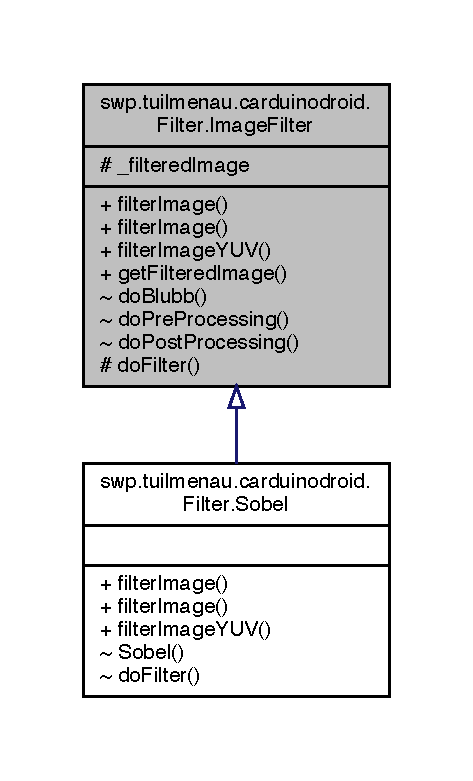
\includegraphics[width=227pt]{classswp_1_1tuilmenau_1_1carduinodroid_1_1_filter_1_1_image_filter__inherit__graph}
\end{center}
\end{figure}


Collaboration diagram for swp.\+tuilmenau.\+carduinodroid.\+Filter.\+Image\+Filter\+:
\nopagebreak
\begin{figure}[H]
\begin{center}
\leavevmode
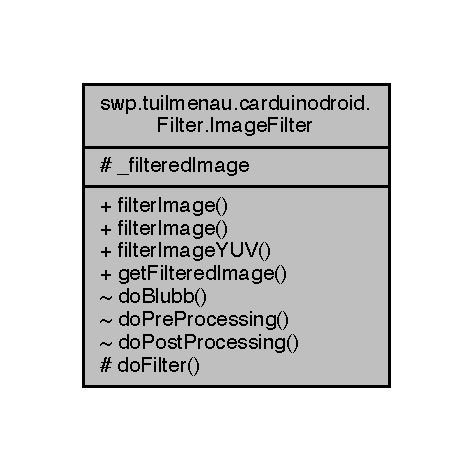
\includegraphics[width=227pt]{classswp_1_1tuilmenau_1_1carduinodroid_1_1_filter_1_1_image_filter__coll__graph}
\end{center}
\end{figure}
\subsection*{Public Member Functions}
\begin{DoxyCompactItemize}
\item 
abstract Bitmap \hyperlink{classswp_1_1tuilmenau_1_1carduinodroid_1_1_filter_1_1_image_filter_afe4620095971cd9f370dea4ef4927bbc}{filter\+Image} (byte\mbox{[}$\,$\mbox{]} data)
\item 
abstract Bitmap \hyperlink{classswp_1_1tuilmenau_1_1carduinodroid_1_1_filter_1_1_image_filter_a53502ae5b361e9c5aafb0ef8e1c114b2}{filter\+Image} (byte\mbox{[}$\,$\mbox{]} data, int width, int height)
\item 
abstract Yuv\+Image \hyperlink{classswp_1_1tuilmenau_1_1carduinodroid_1_1_filter_1_1_image_filter_a1b9f146096c5a3364ea740f770470722}{filter\+Image\+Y\+U\+V} (byte\mbox{[}$\,$\mbox{]} data, int width, int height)
\item 
byte\mbox{[}$\,$\mbox{]} \hyperlink{classswp_1_1tuilmenau_1_1carduinodroid_1_1_filter_1_1_image_filter_a96a2cfa716c71ec05a118c664e63bfe5}{get\+Filtered\+Image} ()
\end{DoxyCompactItemize}
\subsection*{Protected Member Functions}
\begin{DoxyCompactItemize}
\item 
abstract$<$ T $>$ void \hyperlink{classswp_1_1tuilmenau_1_1carduinodroid_1_1_filter_1_1_image_filter_a9f116db5e228c51c7b8d8b9bcdba7ac4}{do\+Filter} (byte\mbox{[}$\,$\mbox{]} data, Class$<$ T $>$ clazz)
\end{DoxyCompactItemize}
\subsection*{Protected Attributes}
\begin{DoxyCompactItemize}
\item 
byte\mbox{[}$\,$\mbox{]} \hyperlink{classswp_1_1tuilmenau_1_1carduinodroid_1_1_filter_1_1_image_filter_adbb999f81181d3265e5743f6628d42c3}{\+\_\+filtered\+Image}
\end{DoxyCompactItemize}


\subsection{Member Function Documentation}
\hypertarget{classswp_1_1tuilmenau_1_1carduinodroid_1_1_filter_1_1_image_filter_a9f116db5e228c51c7b8d8b9bcdba7ac4}{}\index{swp\+::tuilmenau\+::carduinodroid\+::\+Filter\+::\+Image\+Filter@{swp\+::tuilmenau\+::carduinodroid\+::\+Filter\+::\+Image\+Filter}!do\+Filter@{do\+Filter}}
\index{do\+Filter@{do\+Filter}!swp\+::tuilmenau\+::carduinodroid\+::\+Filter\+::\+Image\+Filter@{swp\+::tuilmenau\+::carduinodroid\+::\+Filter\+::\+Image\+Filter}}
\subsubsection[{do\+Filter}]{\setlength{\rightskip}{0pt plus 5cm}abstract $<$T$>$ void swp.\+tuilmenau.\+carduinodroid.\+Filter.\+Image\+Filter.\+do\+Filter (
\begin{DoxyParamCaption}
\item[{byte\mbox{[}$\,$\mbox{]}}]{data, }
\item[{Class$<$ T $>$}]{clazz}
\end{DoxyParamCaption}
)\hspace{0.3cm}{\ttfamily [abstract]}, {\ttfamily [protected]}}\label{classswp_1_1tuilmenau_1_1carduinodroid_1_1_filter_1_1_image_filter_a9f116db5e228c51c7b8d8b9bcdba7ac4}
\hypertarget{classswp_1_1tuilmenau_1_1carduinodroid_1_1_filter_1_1_image_filter_afe4620095971cd9f370dea4ef4927bbc}{}\index{swp\+::tuilmenau\+::carduinodroid\+::\+Filter\+::\+Image\+Filter@{swp\+::tuilmenau\+::carduinodroid\+::\+Filter\+::\+Image\+Filter}!filter\+Image@{filter\+Image}}
\index{filter\+Image@{filter\+Image}!swp\+::tuilmenau\+::carduinodroid\+::\+Filter\+::\+Image\+Filter@{swp\+::tuilmenau\+::carduinodroid\+::\+Filter\+::\+Image\+Filter}}
\subsubsection[{filter\+Image}]{\setlength{\rightskip}{0pt plus 5cm}abstract Bitmap swp.\+tuilmenau.\+carduinodroid.\+Filter.\+Image\+Filter.\+filter\+Image (
\begin{DoxyParamCaption}
\item[{byte\mbox{[}$\,$\mbox{]}}]{data}
\end{DoxyParamCaption}
)\hspace{0.3cm}{\ttfamily [abstract]}}\label{classswp_1_1tuilmenau_1_1carduinodroid_1_1_filter_1_1_image_filter_afe4620095971cd9f370dea4ef4927bbc}

\begin{DoxyParams}{Parameters}
{\em data} & \\
\hline
\end{DoxyParams}
\begin{DoxyReturn}{Returns}

\end{DoxyReturn}
\hypertarget{classswp_1_1tuilmenau_1_1carduinodroid_1_1_filter_1_1_image_filter_a53502ae5b361e9c5aafb0ef8e1c114b2}{}\index{swp\+::tuilmenau\+::carduinodroid\+::\+Filter\+::\+Image\+Filter@{swp\+::tuilmenau\+::carduinodroid\+::\+Filter\+::\+Image\+Filter}!filter\+Image@{filter\+Image}}
\index{filter\+Image@{filter\+Image}!swp\+::tuilmenau\+::carduinodroid\+::\+Filter\+::\+Image\+Filter@{swp\+::tuilmenau\+::carduinodroid\+::\+Filter\+::\+Image\+Filter}}
\subsubsection[{filter\+Image}]{\setlength{\rightskip}{0pt plus 5cm}abstract Bitmap swp.\+tuilmenau.\+carduinodroid.\+Filter.\+Image\+Filter.\+filter\+Image (
\begin{DoxyParamCaption}
\item[{byte\mbox{[}$\,$\mbox{]}}]{data, }
\item[{int}]{width, }
\item[{int}]{height}
\end{DoxyParamCaption}
)\hspace{0.3cm}{\ttfamily [abstract]}}\label{classswp_1_1tuilmenau_1_1carduinodroid_1_1_filter_1_1_image_filter_a53502ae5b361e9c5aafb0ef8e1c114b2}
\hypertarget{classswp_1_1tuilmenau_1_1carduinodroid_1_1_filter_1_1_image_filter_a1b9f146096c5a3364ea740f770470722}{}\index{swp\+::tuilmenau\+::carduinodroid\+::\+Filter\+::\+Image\+Filter@{swp\+::tuilmenau\+::carduinodroid\+::\+Filter\+::\+Image\+Filter}!filter\+Image\+Y\+U\+V@{filter\+Image\+Y\+U\+V}}
\index{filter\+Image\+Y\+U\+V@{filter\+Image\+Y\+U\+V}!swp\+::tuilmenau\+::carduinodroid\+::\+Filter\+::\+Image\+Filter@{swp\+::tuilmenau\+::carduinodroid\+::\+Filter\+::\+Image\+Filter}}
\subsubsection[{filter\+Image\+Y\+U\+V}]{\setlength{\rightskip}{0pt plus 5cm}abstract Yuv\+Image swp.\+tuilmenau.\+carduinodroid.\+Filter.\+Image\+Filter.\+filter\+Image\+Y\+U\+V (
\begin{DoxyParamCaption}
\item[{byte\mbox{[}$\,$\mbox{]}}]{data, }
\item[{int}]{width, }
\item[{int}]{height}
\end{DoxyParamCaption}
)\hspace{0.3cm}{\ttfamily [abstract]}}\label{classswp_1_1tuilmenau_1_1carduinodroid_1_1_filter_1_1_image_filter_a1b9f146096c5a3364ea740f770470722}


Here is the caller graph for this function\+:
\nopagebreak
\begin{figure}[H]
\begin{center}
\leavevmode
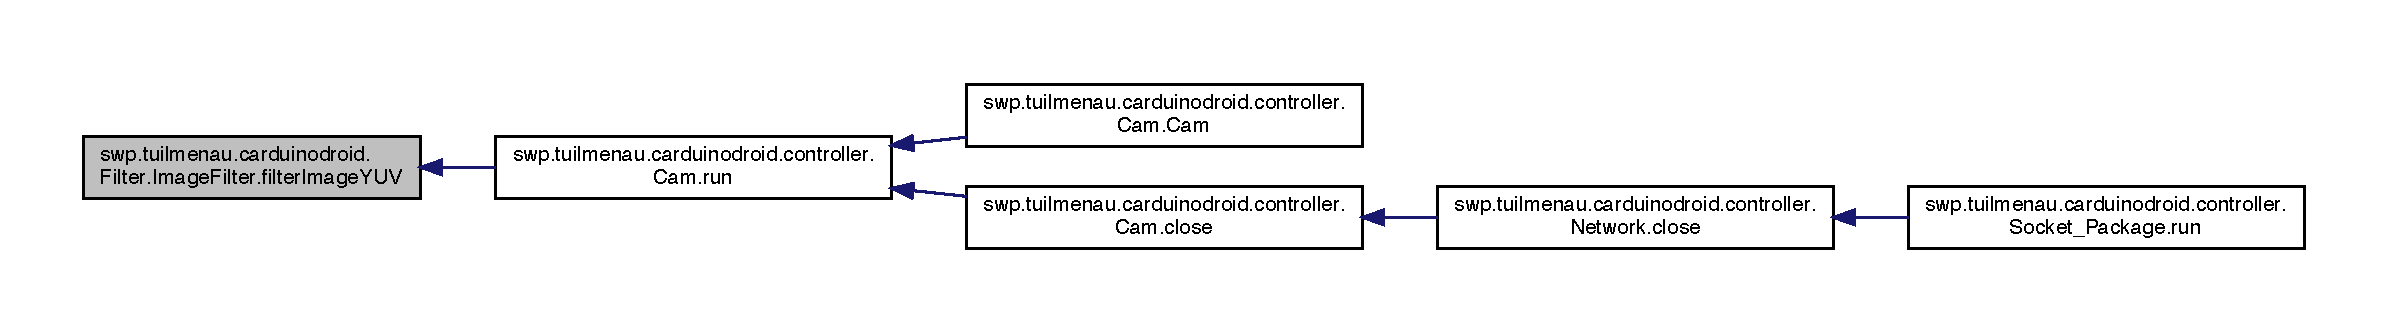
\includegraphics[width=350pt]{classswp_1_1tuilmenau_1_1carduinodroid_1_1_filter_1_1_image_filter_a1b9f146096c5a3364ea740f770470722_icgraph}
\end{center}
\end{figure}


\hypertarget{classswp_1_1tuilmenau_1_1carduinodroid_1_1_filter_1_1_image_filter_a96a2cfa716c71ec05a118c664e63bfe5}{}\index{swp\+::tuilmenau\+::carduinodroid\+::\+Filter\+::\+Image\+Filter@{swp\+::tuilmenau\+::carduinodroid\+::\+Filter\+::\+Image\+Filter}!get\+Filtered\+Image@{get\+Filtered\+Image}}
\index{get\+Filtered\+Image@{get\+Filtered\+Image}!swp\+::tuilmenau\+::carduinodroid\+::\+Filter\+::\+Image\+Filter@{swp\+::tuilmenau\+::carduinodroid\+::\+Filter\+::\+Image\+Filter}}
\subsubsection[{get\+Filtered\+Image}]{\setlength{\rightskip}{0pt plus 5cm}byte \mbox{[}$\,$\mbox{]} swp.\+tuilmenau.\+carduinodroid.\+Filter.\+Image\+Filter.\+get\+Filtered\+Image (
\begin{DoxyParamCaption}
{}
\end{DoxyParamCaption}
)}\label{classswp_1_1tuilmenau_1_1carduinodroid_1_1_filter_1_1_image_filter_a96a2cfa716c71ec05a118c664e63bfe5}


\subsection{Member Data Documentation}
\hypertarget{classswp_1_1tuilmenau_1_1carduinodroid_1_1_filter_1_1_image_filter_adbb999f81181d3265e5743f6628d42c3}{}\index{swp\+::tuilmenau\+::carduinodroid\+::\+Filter\+::\+Image\+Filter@{swp\+::tuilmenau\+::carduinodroid\+::\+Filter\+::\+Image\+Filter}!\+\_\+filtered\+Image@{\+\_\+filtered\+Image}}
\index{\+\_\+filtered\+Image@{\+\_\+filtered\+Image}!swp\+::tuilmenau\+::carduinodroid\+::\+Filter\+::\+Image\+Filter@{swp\+::tuilmenau\+::carduinodroid\+::\+Filter\+::\+Image\+Filter}}
\subsubsection[{\+\_\+filtered\+Image}]{\setlength{\rightskip}{0pt plus 5cm}byte \mbox{[}$\,$\mbox{]} swp.\+tuilmenau.\+carduinodroid.\+Filter.\+Image\+Filter.\+\_\+filtered\+Image\hspace{0.3cm}{\ttfamily [protected]}}\label{classswp_1_1tuilmenau_1_1carduinodroid_1_1_filter_1_1_image_filter_adbb999f81181d3265e5743f6628d42c3}


The documentation for this class was generated from the following file\+:\begin{DoxyCompactItemize}
\item 
src/swp/tuilmenau/carduinodroid/\+Filter/\hyperlink{_image_filter_8java}{Image\+Filter.\+java}\end{DoxyCompactItemize}

\hypertarget{interfaceswp_1_1tuilmenau_1_1carduinodroid_1_1controller_1_1_i_usb_connection_handler}{}\section{swp.\+tuilmenau.\+carduinodroid.\+controller.\+I\+Usb\+Connection\+Handler Interface Reference}
\label{interfaceswp_1_1tuilmenau_1_1carduinodroid_1_1controller_1_1_i_usb_connection_handler}\index{swp.\+tuilmenau.\+carduinodroid.\+controller.\+I\+Usb\+Connection\+Handler@{swp.\+tuilmenau.\+carduinodroid.\+controller.\+I\+Usb\+Connection\+Handler}}


Collaboration diagram for swp.\+tuilmenau.\+carduinodroid.\+controller.\+I\+Usb\+Connection\+Handler\+:
\nopagebreak
\begin{figure}[H]
\begin{center}
\leavevmode
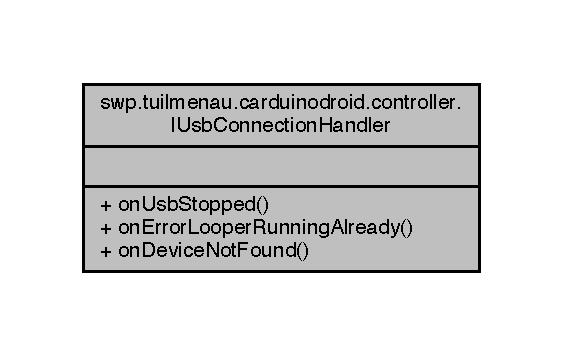
\includegraphics[width=270pt]{interfaceswp_1_1tuilmenau_1_1carduinodroid_1_1controller_1_1_i_usb_connection_handler__coll__graph}
\end{center}
\end{figure}
\subsection*{Public Member Functions}
\begin{DoxyCompactItemize}
\item 
void \hyperlink{interfaceswp_1_1tuilmenau_1_1carduinodroid_1_1controller_1_1_i_usb_connection_handler_a1bb25ee474b0c65e5cac68f504e3322b}{on\+Usb\+Stopped} ()
\item 
void \hyperlink{interfaceswp_1_1tuilmenau_1_1carduinodroid_1_1controller_1_1_i_usb_connection_handler_afcaf80567470dce1b025832862b5193a}{on\+Error\+Looper\+Running\+Already} ()
\item 
void \hyperlink{interfaceswp_1_1tuilmenau_1_1carduinodroid_1_1controller_1_1_i_usb_connection_handler_a28256f61b093f0a19946f5f822861225}{on\+Device\+Not\+Found} ()
\end{DoxyCompactItemize}


\subsection{Member Function Documentation}
\hypertarget{interfaceswp_1_1tuilmenau_1_1carduinodroid_1_1controller_1_1_i_usb_connection_handler_a28256f61b093f0a19946f5f822861225}{}\index{swp\+::tuilmenau\+::carduinodroid\+::controller\+::\+I\+Usb\+Connection\+Handler@{swp\+::tuilmenau\+::carduinodroid\+::controller\+::\+I\+Usb\+Connection\+Handler}!on\+Device\+Not\+Found@{on\+Device\+Not\+Found}}
\index{on\+Device\+Not\+Found@{on\+Device\+Not\+Found}!swp\+::tuilmenau\+::carduinodroid\+::controller\+::\+I\+Usb\+Connection\+Handler@{swp\+::tuilmenau\+::carduinodroid\+::controller\+::\+I\+Usb\+Connection\+Handler}}
\subsubsection[{on\+Device\+Not\+Found}]{\setlength{\rightskip}{0pt plus 5cm}void swp.\+tuilmenau.\+carduinodroid.\+controller.\+I\+Usb\+Connection\+Handler.\+on\+Device\+Not\+Found (
\begin{DoxyParamCaption}
{}
\end{DoxyParamCaption}
)}\label{interfaceswp_1_1tuilmenau_1_1carduinodroid_1_1controller_1_1_i_usb_connection_handler_a28256f61b093f0a19946f5f822861225}
\hypertarget{interfaceswp_1_1tuilmenau_1_1carduinodroid_1_1controller_1_1_i_usb_connection_handler_afcaf80567470dce1b025832862b5193a}{}\index{swp\+::tuilmenau\+::carduinodroid\+::controller\+::\+I\+Usb\+Connection\+Handler@{swp\+::tuilmenau\+::carduinodroid\+::controller\+::\+I\+Usb\+Connection\+Handler}!on\+Error\+Looper\+Running\+Already@{on\+Error\+Looper\+Running\+Already}}
\index{on\+Error\+Looper\+Running\+Already@{on\+Error\+Looper\+Running\+Already}!swp\+::tuilmenau\+::carduinodroid\+::controller\+::\+I\+Usb\+Connection\+Handler@{swp\+::tuilmenau\+::carduinodroid\+::controller\+::\+I\+Usb\+Connection\+Handler}}
\subsubsection[{on\+Error\+Looper\+Running\+Already}]{\setlength{\rightskip}{0pt plus 5cm}void swp.\+tuilmenau.\+carduinodroid.\+controller.\+I\+Usb\+Connection\+Handler.\+on\+Error\+Looper\+Running\+Already (
\begin{DoxyParamCaption}
{}
\end{DoxyParamCaption}
)}\label{interfaceswp_1_1tuilmenau_1_1carduinodroid_1_1controller_1_1_i_usb_connection_handler_afcaf80567470dce1b025832862b5193a}
\hypertarget{interfaceswp_1_1tuilmenau_1_1carduinodroid_1_1controller_1_1_i_usb_connection_handler_a1bb25ee474b0c65e5cac68f504e3322b}{}\index{swp\+::tuilmenau\+::carduinodroid\+::controller\+::\+I\+Usb\+Connection\+Handler@{swp\+::tuilmenau\+::carduinodroid\+::controller\+::\+I\+Usb\+Connection\+Handler}!on\+Usb\+Stopped@{on\+Usb\+Stopped}}
\index{on\+Usb\+Stopped@{on\+Usb\+Stopped}!swp\+::tuilmenau\+::carduinodroid\+::controller\+::\+I\+Usb\+Connection\+Handler@{swp\+::tuilmenau\+::carduinodroid\+::controller\+::\+I\+Usb\+Connection\+Handler}}
\subsubsection[{on\+Usb\+Stopped}]{\setlength{\rightskip}{0pt plus 5cm}void swp.\+tuilmenau.\+carduinodroid.\+controller.\+I\+Usb\+Connection\+Handler.\+on\+Usb\+Stopped (
\begin{DoxyParamCaption}
{}
\end{DoxyParamCaption}
)}\label{interfaceswp_1_1tuilmenau_1_1carduinodroid_1_1controller_1_1_i_usb_connection_handler_a1bb25ee474b0c65e5cac68f504e3322b}


The documentation for this interface was generated from the following file\+:\begin{DoxyCompactItemize}
\item 
src/swp/tuilmenau/carduinodroid/controller/\hyperlink{_i_usb_connection_handler_8java}{I\+Usb\+Connection\+Handler.\+java}\end{DoxyCompactItemize}

\hypertarget{classswp_1_1tuilmenau_1_1carduinodroid_1_1model_1_1_l_o_g}{}\section{swp.\+tuilmenau.\+carduinodroid.\+model.\+L\+O\+G Class Reference}
\label{classswp_1_1tuilmenau_1_1carduinodroid_1_1model_1_1_l_o_g}\index{swp.\+tuilmenau.\+carduinodroid.\+model.\+L\+O\+G@{swp.\+tuilmenau.\+carduinodroid.\+model.\+L\+O\+G}}
\subsection*{Public Member Functions}
\begin{DoxyCompactItemize}
\item 
\hyperlink{classswp_1_1tuilmenau_1_1carduinodroid_1_1model_1_1_l_o_g_a56023f651e46d2187d3103b08781c487}{L\+O\+G} ()
\item 
synchronized void \hyperlink{classswp_1_1tuilmenau_1_1carduinodroid_1_1model_1_1_l_o_g_a07a373e26dd4618bab84def0c899635a}{write} (int type, String line)
\item 
void \hyperlink{classswp_1_1tuilmenau_1_1carduinodroid_1_1model_1_1_l_o_g_af5353ab3a1312b1078ca115fa6e96fcf}{set\+Level} (int lvl)
\item 
void \hyperlink{classswp_1_1tuilmenau_1_1carduinodroid_1_1model_1_1_l_o_g_aaff09fa233326c5968dac4aa2bda4442}{save} ()
\item 
\hyperlink{classswp_1_1tuilmenau_1_1carduinodroid_1_1model_1_1_l_o_g_a56023f651e46d2187d3103b08781c487}{L\+O\+G} ()
\item 
synchronized void \hyperlink{classswp_1_1tuilmenau_1_1carduinodroid_1_1model_1_1_l_o_g_a07a373e26dd4618bab84def0c899635a}{write} (int type, String line)
\item 
void \hyperlink{classswp_1_1tuilmenau_1_1carduinodroid_1_1model_1_1_l_o_g_af5353ab3a1312b1078ca115fa6e96fcf}{set\+Level} (int lvl)
\item 
void \hyperlink{classswp_1_1tuilmenau_1_1carduinodroid_1_1model_1_1_l_o_g_aaff09fa233326c5968dac4aa2bda4442}{save} ()
\end{DoxyCompactItemize}
\subsection*{Static Public Attributes}
\begin{DoxyCompactItemize}
\item 
static final int \hyperlink{classswp_1_1tuilmenau_1_1carduinodroid_1_1model_1_1_l_o_g_afff29e0c91f6559acbe2e9a26b523260}{L\+O\+G\+\_\+\+A\+L\+L} = 1
\item 
static final int \hyperlink{classswp_1_1tuilmenau_1_1carduinodroid_1_1model_1_1_l_o_g_a8b2cb22699bc53122a71cc3e579c515e}{L\+O\+G\+\_\+\+W\+A\+R\+N\+I\+N\+G\+S\+\_\+\+O\+N\+L\+Y} = 2
\item 
static final int \hyperlink{classswp_1_1tuilmenau_1_1carduinodroid_1_1model_1_1_l_o_g_a5a782d2e690478a0f5b8991711ff50be}{I\+N\+F\+O} = 3
\item 
static final int \hyperlink{classswp_1_1tuilmenau_1_1carduinodroid_1_1model_1_1_l_o_g_a533bd3ed6164b71fdb7c48a238207130}{W\+A\+R\+N\+I\+N\+G} = 4
\end{DoxyCompactItemize}


\subsection{Detailed Description}
Provides the global L\+O\+G-\/functionality used by all other subclasses.

\begin{DoxyAuthor}{Author}
Paul Thorwirth 
\end{DoxyAuthor}
\begin{DoxyVersion}{Version}
1.\+0 
\end{DoxyVersion}
\begin{DoxySeeAlso}{See also}
File 

File\+Writer 

Buffered\+Writer 
\end{DoxySeeAlso}


Definition at line 20 of file L\+O\+G.\+java.



\subsection{Constructor \& Destructor Documentation}
\hypertarget{classswp_1_1tuilmenau_1_1carduinodroid_1_1model_1_1_l_o_g_a56023f651e46d2187d3103b08781c487}{}\index{swp\+::tuilmenau\+::carduinodroid\+::model\+::\+L\+O\+G@{swp\+::tuilmenau\+::carduinodroid\+::model\+::\+L\+O\+G}!L\+O\+G@{L\+O\+G}}
\index{L\+O\+G@{L\+O\+G}!swp\+::tuilmenau\+::carduinodroid\+::model\+::\+L\+O\+G@{swp\+::tuilmenau\+::carduinodroid\+::model\+::\+L\+O\+G}}
\subsubsection[{L\+O\+G}]{\setlength{\rightskip}{0pt plus 5cm}swp.\+tuilmenau.\+carduinodroid.\+model.\+L\+O\+G.\+L\+O\+G (
\begin{DoxyParamCaption}
{}
\end{DoxyParamCaption}
)}\label{classswp_1_1tuilmenau_1_1carduinodroid_1_1model_1_1_l_o_g_a56023f651e46d2187d3103b08781c487}
Creates the directories and the file required for logging. 

Definition at line 37 of file L\+O\+G.\+java.



Here is the call graph for this function\+:
% FIG 0


\hypertarget{classswp_1_1tuilmenau_1_1carduinodroid_1_1model_1_1_l_o_g_a56023f651e46d2187d3103b08781c487}{}\index{swp\+::tuilmenau\+::carduinodroid\+::model\+::\+L\+O\+G@{swp\+::tuilmenau\+::carduinodroid\+::model\+::\+L\+O\+G}!L\+O\+G@{L\+O\+G}}
\index{L\+O\+G@{L\+O\+G}!swp\+::tuilmenau\+::carduinodroid\+::model\+::\+L\+O\+G@{swp\+::tuilmenau\+::carduinodroid\+::model\+::\+L\+O\+G}}
\subsubsection[{L\+O\+G}]{\setlength{\rightskip}{0pt plus 5cm}swp.\+tuilmenau.\+carduinodroid.\+model.\+L\+O\+G.\+L\+O\+G (
\begin{DoxyParamCaption}
{}
\end{DoxyParamCaption}
)}\label{classswp_1_1tuilmenau_1_1carduinodroid_1_1model_1_1_l_o_g_a56023f651e46d2187d3103b08781c487}
Creates the directories and the file required for logging. 

Definition at line 37 of file L\+O\+G.\+java.



Here is the call graph for this function\+:
% FIG 1




\subsection{Member Function Documentation}
\hypertarget{classswp_1_1tuilmenau_1_1carduinodroid_1_1model_1_1_l_o_g_aaff09fa233326c5968dac4aa2bda4442}{}\index{swp\+::tuilmenau\+::carduinodroid\+::model\+::\+L\+O\+G@{swp\+::tuilmenau\+::carduinodroid\+::model\+::\+L\+O\+G}!save@{save}}
\index{save@{save}!swp\+::tuilmenau\+::carduinodroid\+::model\+::\+L\+O\+G@{swp\+::tuilmenau\+::carduinodroid\+::model\+::\+L\+O\+G}}
\subsubsection[{save}]{\setlength{\rightskip}{0pt plus 5cm}void swp.\+tuilmenau.\+carduinodroid.\+model.\+L\+O\+G.\+save (
\begin{DoxyParamCaption}
{}
\end{DoxyParamCaption}
)}\label{classswp_1_1tuilmenau_1_1carduinodroid_1_1model_1_1_l_o_g_aaff09fa233326c5968dac4aa2bda4442}
Closes and saves the L\+O\+G-\/\+File.


\begin{DoxyParams}{Parameters}
{\em lvl} & Contains the L\+O\+G-\/\+Level to be set \\
\hline
\end{DoxyParams}


Definition at line 111 of file L\+O\+G.\+java.



Here is the call graph for this function\+:
% FIG 2


\hypertarget{classswp_1_1tuilmenau_1_1carduinodroid_1_1model_1_1_l_o_g_aaff09fa233326c5968dac4aa2bda4442}{}\index{swp\+::tuilmenau\+::carduinodroid\+::model\+::\+L\+O\+G@{swp\+::tuilmenau\+::carduinodroid\+::model\+::\+L\+O\+G}!save@{save}}
\index{save@{save}!swp\+::tuilmenau\+::carduinodroid\+::model\+::\+L\+O\+G@{swp\+::tuilmenau\+::carduinodroid\+::model\+::\+L\+O\+G}}
\subsubsection[{save}]{\setlength{\rightskip}{0pt plus 5cm}void swp.\+tuilmenau.\+carduinodroid.\+model.\+L\+O\+G.\+save (
\begin{DoxyParamCaption}
{}
\end{DoxyParamCaption}
)}\label{classswp_1_1tuilmenau_1_1carduinodroid_1_1model_1_1_l_o_g_aaff09fa233326c5968dac4aa2bda4442}
Closes and saves the L\+O\+G-\/\+File.


\begin{DoxyParams}{Parameters}
{\em lvl} & Contains the L\+O\+G-\/\+Level to be set \\
\hline
\end{DoxyParams}


Definition at line 111 of file L\+O\+G.\+java.



Here is the call graph for this function\+:
% FIG 3


\hypertarget{classswp_1_1tuilmenau_1_1carduinodroid_1_1model_1_1_l_o_g_af5353ab3a1312b1078ca115fa6e96fcf}{}\index{swp\+::tuilmenau\+::carduinodroid\+::model\+::\+L\+O\+G@{swp\+::tuilmenau\+::carduinodroid\+::model\+::\+L\+O\+G}!set\+Level@{set\+Level}}
\index{set\+Level@{set\+Level}!swp\+::tuilmenau\+::carduinodroid\+::model\+::\+L\+O\+G@{swp\+::tuilmenau\+::carduinodroid\+::model\+::\+L\+O\+G}}
\subsubsection[{set\+Level}]{\setlength{\rightskip}{0pt plus 5cm}void swp.\+tuilmenau.\+carduinodroid.\+model.\+L\+O\+G.\+set\+Level (
\begin{DoxyParamCaption}
\item[{int}]{lvl}
\end{DoxyParamCaption}
)}\label{classswp_1_1tuilmenau_1_1carduinodroid_1_1model_1_1_l_o_g_af5353ab3a1312b1078ca115fa6e96fcf}
Sets the L\+O\+G-\/\+Level to either {\itshape L\+O\+G\+\_\+\+A\+L\+L} or {\itshape L\+O\+G\+\_\+\+W\+A\+R\+N\+I\+N\+G\+S\+\_\+\+O\+N\+L\+Y} .


\begin{DoxyParams}{Parameters}
{\em lvl} & Contains the L\+O\+G-\/\+Level to be set \\
\hline
\end{DoxyParams}


Definition at line 101 of file L\+O\+G.\+java.

\hypertarget{classswp_1_1tuilmenau_1_1carduinodroid_1_1model_1_1_l_o_g_af5353ab3a1312b1078ca115fa6e96fcf}{}\index{swp\+::tuilmenau\+::carduinodroid\+::model\+::\+L\+O\+G@{swp\+::tuilmenau\+::carduinodroid\+::model\+::\+L\+O\+G}!set\+Level@{set\+Level}}
\index{set\+Level@{set\+Level}!swp\+::tuilmenau\+::carduinodroid\+::model\+::\+L\+O\+G@{swp\+::tuilmenau\+::carduinodroid\+::model\+::\+L\+O\+G}}
\subsubsection[{set\+Level}]{\setlength{\rightskip}{0pt plus 5cm}void swp.\+tuilmenau.\+carduinodroid.\+model.\+L\+O\+G.\+set\+Level (
\begin{DoxyParamCaption}
\item[{int}]{lvl}
\end{DoxyParamCaption}
)}\label{classswp_1_1tuilmenau_1_1carduinodroid_1_1model_1_1_l_o_g_af5353ab3a1312b1078ca115fa6e96fcf}
Sets the L\+O\+G-\/\+Level to either {\itshape L\+O\+G\+\_\+\+A\+L\+L} or {\itshape L\+O\+G\+\_\+\+W\+A\+R\+N\+I\+N\+G\+S\+\_\+\+O\+N\+L\+Y} .


\begin{DoxyParams}{Parameters}
{\em lvl} & Contains the L\+O\+G-\/\+Level to be set \\
\hline
\end{DoxyParams}


Definition at line 101 of file L\+O\+G.\+java.



Here is the caller graph for this function\+:
% FIG 4


\hypertarget{classswp_1_1tuilmenau_1_1carduinodroid_1_1model_1_1_l_o_g_a07a373e26dd4618bab84def0c899635a}{}\index{swp\+::tuilmenau\+::carduinodroid\+::model\+::\+L\+O\+G@{swp\+::tuilmenau\+::carduinodroid\+::model\+::\+L\+O\+G}!write@{write}}
\index{write@{write}!swp\+::tuilmenau\+::carduinodroid\+::model\+::\+L\+O\+G@{swp\+::tuilmenau\+::carduinodroid\+::model\+::\+L\+O\+G}}
\subsubsection[{write}]{\setlength{\rightskip}{0pt plus 5cm}synchronized void swp.\+tuilmenau.\+carduinodroid.\+model.\+L\+O\+G.\+write (
\begin{DoxyParamCaption}
\item[{int}]{type, }
\item[{String}]{line}
\end{DoxyParamCaption}
)}\label{classswp_1_1tuilmenau_1_1carduinodroid_1_1model_1_1_l_o_g_a07a373e26dd4618bab84def0c899635a}
Writes a new line to the L\+O\+G-\/\+File.


\begin{DoxyParams}{Parameters}
{\em type} & Tag the line to be either W\+A\+R\+N\+I\+N\+G or I\+N\+F\+O \\
\hline
{\em line} & The String to be written to the \hyperlink{classswp_1_1tuilmenau_1_1carduinodroid_1_1model_1_1_l_o_g}{L\+O\+G} \\
\hline
\end{DoxyParams}
\begin{DoxySeeAlso}{See also}
\hyperlink{classswp_1_1tuilmenau_1_1carduinodroid_1_1model_1_1_l_o_g_af5353ab3a1312b1078ca115fa6e96fcf}{set\+Level()} 
\end{DoxySeeAlso}


Definition at line 65 of file L\+O\+G.\+java.

\hypertarget{classswp_1_1tuilmenau_1_1carduinodroid_1_1model_1_1_l_o_g_a07a373e26dd4618bab84def0c899635a}{}\index{swp\+::tuilmenau\+::carduinodroid\+::model\+::\+L\+O\+G@{swp\+::tuilmenau\+::carduinodroid\+::model\+::\+L\+O\+G}!write@{write}}
\index{write@{write}!swp\+::tuilmenau\+::carduinodroid\+::model\+::\+L\+O\+G@{swp\+::tuilmenau\+::carduinodroid\+::model\+::\+L\+O\+G}}
\subsubsection[{write}]{\setlength{\rightskip}{0pt plus 5cm}synchronized void swp.\+tuilmenau.\+carduinodroid.\+model.\+L\+O\+G.\+write (
\begin{DoxyParamCaption}
\item[{int}]{type, }
\item[{String}]{line}
\end{DoxyParamCaption}
)}\label{classswp_1_1tuilmenau_1_1carduinodroid_1_1model_1_1_l_o_g_a07a373e26dd4618bab84def0c899635a}
Writes a new line to the L\+O\+G-\/\+File.


\begin{DoxyParams}{Parameters}
{\em type} & Tag the line to be either W\+A\+R\+N\+I\+N\+G or I\+N\+F\+O \\
\hline
{\em line} & The String to be written to the \hyperlink{classswp_1_1tuilmenau_1_1carduinodroid_1_1model_1_1_l_o_g}{L\+O\+G} \\
\hline
\end{DoxyParams}
\begin{DoxySeeAlso}{See also}
\hyperlink{classswp_1_1tuilmenau_1_1carduinodroid_1_1model_1_1_l_o_g_af5353ab3a1312b1078ca115fa6e96fcf}{set\+Level()} 
\end{DoxySeeAlso}


Definition at line 65 of file L\+O\+G.\+java.



Here is the caller graph for this function\+:
% FIG 5




\subsection{Member Data Documentation}
\hypertarget{classswp_1_1tuilmenau_1_1carduinodroid_1_1model_1_1_l_o_g_a5a782d2e690478a0f5b8991711ff50be}{}\index{swp\+::tuilmenau\+::carduinodroid\+::model\+::\+L\+O\+G@{swp\+::tuilmenau\+::carduinodroid\+::model\+::\+L\+O\+G}!I\+N\+F\+O@{I\+N\+F\+O}}
\index{I\+N\+F\+O@{I\+N\+F\+O}!swp\+::tuilmenau\+::carduinodroid\+::model\+::\+L\+O\+G@{swp\+::tuilmenau\+::carduinodroid\+::model\+::\+L\+O\+G}}
\subsubsection[{I\+N\+F\+O}]{\setlength{\rightskip}{0pt plus 5cm}static final int swp.\+tuilmenau.\+carduinodroid.\+model.\+L\+O\+G.\+I\+N\+F\+O = 3\hspace{0.3cm}{\ttfamily [static]}}\label{classswp_1_1tuilmenau_1_1carduinodroid_1_1model_1_1_l_o_g_a5a782d2e690478a0f5b8991711ff50be}


Definition at line 24 of file L\+O\+G.\+java.

\hypertarget{classswp_1_1tuilmenau_1_1carduinodroid_1_1model_1_1_l_o_g_afff29e0c91f6559acbe2e9a26b523260}{}\index{swp\+::tuilmenau\+::carduinodroid\+::model\+::\+L\+O\+G@{swp\+::tuilmenau\+::carduinodroid\+::model\+::\+L\+O\+G}!L\+O\+G\+\_\+\+A\+L\+L@{L\+O\+G\+\_\+\+A\+L\+L}}
\index{L\+O\+G\+\_\+\+A\+L\+L@{L\+O\+G\+\_\+\+A\+L\+L}!swp\+::tuilmenau\+::carduinodroid\+::model\+::\+L\+O\+G@{swp\+::tuilmenau\+::carduinodroid\+::model\+::\+L\+O\+G}}
\subsubsection[{L\+O\+G\+\_\+\+A\+L\+L}]{\setlength{\rightskip}{0pt plus 5cm}static final int swp.\+tuilmenau.\+carduinodroid.\+model.\+L\+O\+G.\+L\+O\+G\+\_\+\+A\+L\+L = 1\hspace{0.3cm}{\ttfamily [static]}}\label{classswp_1_1tuilmenau_1_1carduinodroid_1_1model_1_1_l_o_g_afff29e0c91f6559acbe2e9a26b523260}


Definition at line 22 of file L\+O\+G.\+java.

\hypertarget{classswp_1_1tuilmenau_1_1carduinodroid_1_1model_1_1_l_o_g_a8b2cb22699bc53122a71cc3e579c515e}{}\index{swp\+::tuilmenau\+::carduinodroid\+::model\+::\+L\+O\+G@{swp\+::tuilmenau\+::carduinodroid\+::model\+::\+L\+O\+G}!L\+O\+G\+\_\+\+W\+A\+R\+N\+I\+N\+G\+S\+\_\+\+O\+N\+L\+Y@{L\+O\+G\+\_\+\+W\+A\+R\+N\+I\+N\+G\+S\+\_\+\+O\+N\+L\+Y}}
\index{L\+O\+G\+\_\+\+W\+A\+R\+N\+I\+N\+G\+S\+\_\+\+O\+N\+L\+Y@{L\+O\+G\+\_\+\+W\+A\+R\+N\+I\+N\+G\+S\+\_\+\+O\+N\+L\+Y}!swp\+::tuilmenau\+::carduinodroid\+::model\+::\+L\+O\+G@{swp\+::tuilmenau\+::carduinodroid\+::model\+::\+L\+O\+G}}
\subsubsection[{L\+O\+G\+\_\+\+W\+A\+R\+N\+I\+N\+G\+S\+\_\+\+O\+N\+L\+Y}]{\setlength{\rightskip}{0pt plus 5cm}static final int swp.\+tuilmenau.\+carduinodroid.\+model.\+L\+O\+G.\+L\+O\+G\+\_\+\+W\+A\+R\+N\+I\+N\+G\+S\+\_\+\+O\+N\+L\+Y = 2\hspace{0.3cm}{\ttfamily [static]}}\label{classswp_1_1tuilmenau_1_1carduinodroid_1_1model_1_1_l_o_g_a8b2cb22699bc53122a71cc3e579c515e}


Definition at line 23 of file L\+O\+G.\+java.

\hypertarget{classswp_1_1tuilmenau_1_1carduinodroid_1_1model_1_1_l_o_g_a533bd3ed6164b71fdb7c48a238207130}{}\index{swp\+::tuilmenau\+::carduinodroid\+::model\+::\+L\+O\+G@{swp\+::tuilmenau\+::carduinodroid\+::model\+::\+L\+O\+G}!W\+A\+R\+N\+I\+N\+G@{W\+A\+R\+N\+I\+N\+G}}
\index{W\+A\+R\+N\+I\+N\+G@{W\+A\+R\+N\+I\+N\+G}!swp\+::tuilmenau\+::carduinodroid\+::model\+::\+L\+O\+G@{swp\+::tuilmenau\+::carduinodroid\+::model\+::\+L\+O\+G}}
\subsubsection[{W\+A\+R\+N\+I\+N\+G}]{\setlength{\rightskip}{0pt plus 5cm}static final int swp.\+tuilmenau.\+carduinodroid.\+model.\+L\+O\+G.\+W\+A\+R\+N\+I\+N\+G = 4\hspace{0.3cm}{\ttfamily [static]}}\label{classswp_1_1tuilmenau_1_1carduinodroid_1_1model_1_1_l_o_g_a533bd3ed6164b71fdb7c48a238207130}


Definition at line 25 of file L\+O\+G.\+java.



The documentation for this class was generated from the following file\+:\begin{DoxyCompactItemize}
\item 
bin/classes/swp/tuilmenau/carduinodroid/model/\hyperlink{bin_2classes_2swp_2tuilmenau_2carduinodroid_2model_2_l_o_g_8java}{L\+O\+G.\+java}\end{DoxyCompactItemize}

\hypertarget{classswp_1_1tuilmenau_1_1carduinodroid_1_1controller_1_1_my_preview_callback}{}\section{swp.\+tuilmenau.\+carduinodroid.\+controller.\+My\+Preview\+Callback Class Reference}
\label{classswp_1_1tuilmenau_1_1carduinodroid_1_1controller_1_1_my_preview_callback}\index{swp.\+tuilmenau.\+carduinodroid.\+controller.\+My\+Preview\+Callback@{swp.\+tuilmenau.\+carduinodroid.\+controller.\+My\+Preview\+Callback}}


Inheritance diagram for swp.\+tuilmenau.\+carduinodroid.\+controller.\+My\+Preview\+Callback\+:
\nopagebreak
\begin{figure}[H]
\begin{center}
\leavevmode
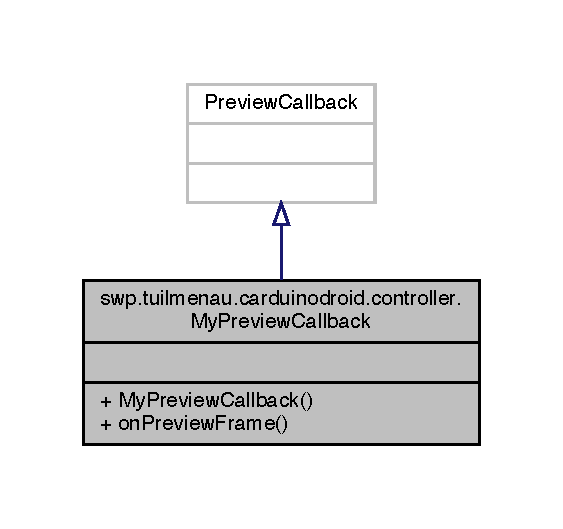
\includegraphics[width=270pt]{classswp_1_1tuilmenau_1_1carduinodroid_1_1controller_1_1_my_preview_callback__inherit__graph}
\end{center}
\end{figure}


Collaboration diagram for swp.\+tuilmenau.\+carduinodroid.\+controller.\+My\+Preview\+Callback\+:
\nopagebreak
\begin{figure}[H]
\begin{center}
\leavevmode
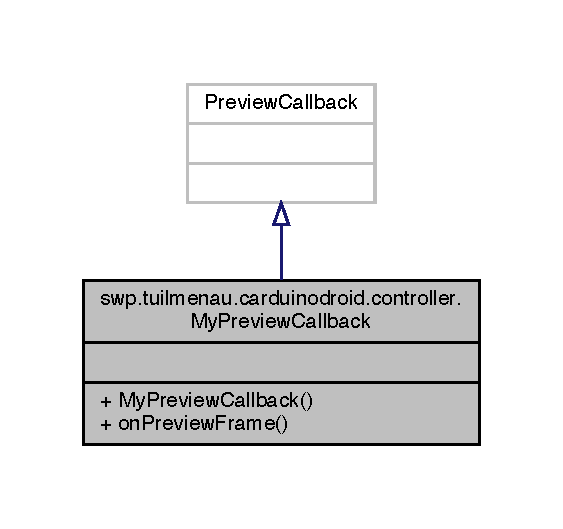
\includegraphics[width=270pt]{classswp_1_1tuilmenau_1_1carduinodroid_1_1controller_1_1_my_preview_callback__coll__graph}
\end{center}
\end{figure}
\subsection*{Public Member Functions}
\begin{DoxyCompactItemize}
\item 
\hyperlink{classswp_1_1tuilmenau_1_1carduinodroid_1_1controller_1_1_my_preview_callback_a7449892b8d437f14fad2694c21014b94}{My\+Preview\+Callback} (\hyperlink{classswp_1_1tuilmenau_1_1carduinodroid_1_1controller_1_1_cam}{Cam} cam)
\item 
void \hyperlink{classswp_1_1tuilmenau_1_1carduinodroid_1_1controller_1_1_my_preview_callback_a74b7673db7b371599752a8c541348852}{on\+Preview\+Frame} (byte\mbox{[}$\,$\mbox{]} data, Camera camera)
\end{DoxyCompactItemize}


\subsection{Constructor \& Destructor Documentation}
\hypertarget{classswp_1_1tuilmenau_1_1carduinodroid_1_1controller_1_1_my_preview_callback_a7449892b8d437f14fad2694c21014b94}{}\index{swp\+::tuilmenau\+::carduinodroid\+::controller\+::\+My\+Preview\+Callback@{swp\+::tuilmenau\+::carduinodroid\+::controller\+::\+My\+Preview\+Callback}!My\+Preview\+Callback@{My\+Preview\+Callback}}
\index{My\+Preview\+Callback@{My\+Preview\+Callback}!swp\+::tuilmenau\+::carduinodroid\+::controller\+::\+My\+Preview\+Callback@{swp\+::tuilmenau\+::carduinodroid\+::controller\+::\+My\+Preview\+Callback}}
\subsubsection[{My\+Preview\+Callback}]{\setlength{\rightskip}{0pt plus 5cm}swp.\+tuilmenau.\+carduinodroid.\+controller.\+My\+Preview\+Callback.\+My\+Preview\+Callback (
\begin{DoxyParamCaption}
\item[{{\bf Cam}}]{cam}
\end{DoxyParamCaption}
)}\label{classswp_1_1tuilmenau_1_1carduinodroid_1_1controller_1_1_my_preview_callback_a7449892b8d437f14fad2694c21014b94}


\subsection{Member Function Documentation}
\hypertarget{classswp_1_1tuilmenau_1_1carduinodroid_1_1controller_1_1_my_preview_callback_a74b7673db7b371599752a8c541348852}{}\index{swp\+::tuilmenau\+::carduinodroid\+::controller\+::\+My\+Preview\+Callback@{swp\+::tuilmenau\+::carduinodroid\+::controller\+::\+My\+Preview\+Callback}!on\+Preview\+Frame@{on\+Preview\+Frame}}
\index{on\+Preview\+Frame@{on\+Preview\+Frame}!swp\+::tuilmenau\+::carduinodroid\+::controller\+::\+My\+Preview\+Callback@{swp\+::tuilmenau\+::carduinodroid\+::controller\+::\+My\+Preview\+Callback}}
\subsubsection[{on\+Preview\+Frame}]{\setlength{\rightskip}{0pt plus 5cm}void swp.\+tuilmenau.\+carduinodroid.\+controller.\+My\+Preview\+Callback.\+on\+Preview\+Frame (
\begin{DoxyParamCaption}
\item[{byte\mbox{[}$\,$\mbox{]}}]{data, }
\item[{Camera}]{camera}
\end{DoxyParamCaption}
)}\label{classswp_1_1tuilmenau_1_1carduinodroid_1_1controller_1_1_my_preview_callback_a74b7673db7b371599752a8c541348852}


Here is the call graph for this function\+:
\nopagebreak
\begin{figure}[H]
\begin{center}
\leavevmode
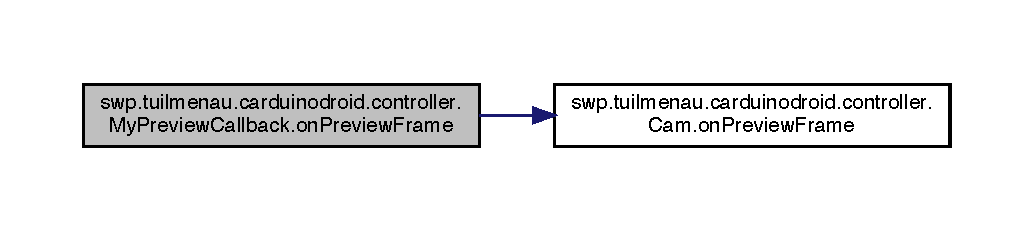
\includegraphics[width=350pt]{classswp_1_1tuilmenau_1_1carduinodroid_1_1controller_1_1_my_preview_callback_a74b7673db7b371599752a8c541348852_cgraph}
\end{center}
\end{figure}




The documentation for this class was generated from the following file\+:\begin{DoxyCompactItemize}
\item 
src/swp/tuilmenau/carduinodroid/controller/\hyperlink{_my_preview_callback_8java}{My\+Preview\+Callback.\+java}\end{DoxyCompactItemize}

\hypertarget{classswp_1_1tuilmenau_1_1carduinodroid_1_1controller_1_1_network}{}\section{swp.\+tuilmenau.\+carduinodroid.\+controller.\+Network Class Reference}
\label{classswp_1_1tuilmenau_1_1carduinodroid_1_1controller_1_1_network}\index{swp.\+tuilmenau.\+carduinodroid.\+controller.\+Network@{swp.\+tuilmenau.\+carduinodroid.\+controller.\+Network}}


Collaboration diagram for swp.\+tuilmenau.\+carduinodroid.\+controller.\+Network\+:
% FIG 0
\subsection*{Public Member Functions}
\begin{DoxyCompactItemize}
\item 
\hyperlink{classswp_1_1tuilmenau_1_1carduinodroid_1_1controller_1_1_network_ab8d4c3dc6072ba6e6d96d0fd6c1b76e2}{Network} (\hyperlink{classswp_1_1tuilmenau_1_1carduinodroid_1_1controller_1_1_controller___android}{Controller\+\_\+\+Android} n\+\_\+controller)
\item 
void \hyperlink{classswp_1_1tuilmenau_1_1carduinodroid_1_1controller_1_1_network_a3bdf599c2a8dfadbe3b2d8e7c00b8ab0}{receive\+\_\+controll} (String message)  throws I\+O\+Exception 
\item 
void \hyperlink{classswp_1_1tuilmenau_1_1carduinodroid_1_1controller_1_1_network_a310032de4956f12176e2ab75d9d34851}{close} ()
\item 
\hyperlink{classswp_1_1tuilmenau_1_1carduinodroid_1_1controller_1_1_network_ab8d4c3dc6072ba6e6d96d0fd6c1b76e2}{Network} (\hyperlink{classswp_1_1tuilmenau_1_1carduinodroid_1_1controller_1_1_controller___android}{Controller\+\_\+\+Android} n\+\_\+controller)
\item 
void \hyperlink{classswp_1_1tuilmenau_1_1carduinodroid_1_1controller_1_1_network_a3bdf599c2a8dfadbe3b2d8e7c00b8ab0}{receive\+\_\+controll} (String message)  throws I\+O\+Exception 
\item 
void \hyperlink{classswp_1_1tuilmenau_1_1carduinodroid_1_1controller_1_1_network_a310032de4956f12176e2ab75d9d34851}{close} ()
\end{DoxyCompactItemize}


\subsection{Detailed Description}
This class is used to start the connection with the pc-\/programm. \begin{DoxyAuthor}{Author}
Robin 
\end{DoxyAuthor}


Definition at line 13 of file Network.\+java.



\subsection{Constructor \& Destructor Documentation}
\hypertarget{classswp_1_1tuilmenau_1_1carduinodroid_1_1controller_1_1_network_ab8d4c3dc6072ba6e6d96d0fd6c1b76e2}{}\index{swp\+::tuilmenau\+::carduinodroid\+::controller\+::\+Network@{swp\+::tuilmenau\+::carduinodroid\+::controller\+::\+Network}!Network@{Network}}
\index{Network@{Network}!swp\+::tuilmenau\+::carduinodroid\+::controller\+::\+Network@{swp\+::tuilmenau\+::carduinodroid\+::controller\+::\+Network}}
\subsubsection[{Network}]{\setlength{\rightskip}{0pt plus 5cm}swp.\+tuilmenau.\+carduinodroid.\+controller.\+Network.\+Network (
\begin{DoxyParamCaption}
\item[{{\bf Controller\+\_\+\+Android}}]{n\+\_\+controller}
\end{DoxyParamCaption}
)}\label{classswp_1_1tuilmenau_1_1carduinodroid_1_1controller_1_1_network_ab8d4c3dc6072ba6e6d96d0fd6c1b76e2}
This is the constructor of the class. It creates a instance of \hyperlink{classswp_1_1tuilmenau_1_1carduinodroid_1_1controller_1_1_socket___controller}{Socket\+\_\+\+Controller} and \hyperlink{classswp_1_1tuilmenau_1_1carduinodroid_1_1controller_1_1_socket___package}{Socket\+\_\+\+Package} 
\begin{DoxyParams}{Parameters}
{\em n\+\_\+controller} & A instance of the \hyperlink{classswp_1_1tuilmenau_1_1carduinodroid_1_1controller_1_1_controller___android}{Controller\+\_\+\+Android} \\
\hline
\end{DoxyParams}


Definition at line 28 of file Network.\+java.



Here is the call graph for this function\+:
% FIG 1


\hypertarget{classswp_1_1tuilmenau_1_1carduinodroid_1_1controller_1_1_network_ab8d4c3dc6072ba6e6d96d0fd6c1b76e2}{}\index{swp\+::tuilmenau\+::carduinodroid\+::controller\+::\+Network@{swp\+::tuilmenau\+::carduinodroid\+::controller\+::\+Network}!Network@{Network}}
\index{Network@{Network}!swp\+::tuilmenau\+::carduinodroid\+::controller\+::\+Network@{swp\+::tuilmenau\+::carduinodroid\+::controller\+::\+Network}}
\subsubsection[{Network}]{\setlength{\rightskip}{0pt plus 5cm}swp.\+tuilmenau.\+carduinodroid.\+controller.\+Network.\+Network (
\begin{DoxyParamCaption}
\item[{{\bf Controller\+\_\+\+Android}}]{n\+\_\+controller}
\end{DoxyParamCaption}
)}\label{classswp_1_1tuilmenau_1_1carduinodroid_1_1controller_1_1_network_ab8d4c3dc6072ba6e6d96d0fd6c1b76e2}
This is the constructor of the class. It creates a instance of \hyperlink{classswp_1_1tuilmenau_1_1carduinodroid_1_1controller_1_1_socket___controller}{Socket\+\_\+\+Controller} and \hyperlink{classswp_1_1tuilmenau_1_1carduinodroid_1_1controller_1_1_socket___package}{Socket\+\_\+\+Package} 
\begin{DoxyParams}{Parameters}
{\em n\+\_\+controller} & A instance of the \hyperlink{classswp_1_1tuilmenau_1_1carduinodroid_1_1controller_1_1_controller___android}{Controller\+\_\+\+Android} \\
\hline
\end{DoxyParams}


Definition at line 28 of file Network.\+java.



Here is the call graph for this function\+:
% FIG 2




\subsection{Member Function Documentation}
\hypertarget{classswp_1_1tuilmenau_1_1carduinodroid_1_1controller_1_1_network_a310032de4956f12176e2ab75d9d34851}{}\index{swp\+::tuilmenau\+::carduinodroid\+::controller\+::\+Network@{swp\+::tuilmenau\+::carduinodroid\+::controller\+::\+Network}!close@{close}}
\index{close@{close}!swp\+::tuilmenau\+::carduinodroid\+::controller\+::\+Network@{swp\+::tuilmenau\+::carduinodroid\+::controller\+::\+Network}}
\subsubsection[{close}]{\setlength{\rightskip}{0pt plus 5cm}void swp.\+tuilmenau.\+carduinodroid.\+controller.\+Network.\+close (
\begin{DoxyParamCaption}
{}
\end{DoxyParamCaption}
)}\label{classswp_1_1tuilmenau_1_1carduinodroid_1_1controller_1_1_network_a310032de4956f12176e2ab75d9d34851}


Definition at line 55 of file Network.\+java.



Here is the call graph for this function\+:
% FIG 3




Here is the caller graph for this function\+:
% FIG 4


\hypertarget{classswp_1_1tuilmenau_1_1carduinodroid_1_1controller_1_1_network_a310032de4956f12176e2ab75d9d34851}{}\index{swp\+::tuilmenau\+::carduinodroid\+::controller\+::\+Network@{swp\+::tuilmenau\+::carduinodroid\+::controller\+::\+Network}!close@{close}}
\index{close@{close}!swp\+::tuilmenau\+::carduinodroid\+::controller\+::\+Network@{swp\+::tuilmenau\+::carduinodroid\+::controller\+::\+Network}}
\subsubsection[{close}]{\setlength{\rightskip}{0pt plus 5cm}void swp.\+tuilmenau.\+carduinodroid.\+controller.\+Network.\+close (
\begin{DoxyParamCaption}
{}
\end{DoxyParamCaption}
)}\label{classswp_1_1tuilmenau_1_1carduinodroid_1_1controller_1_1_network_a310032de4956f12176e2ab75d9d34851}


Definition at line 55 of file Network.\+java.

\hypertarget{classswp_1_1tuilmenau_1_1carduinodroid_1_1controller_1_1_network_a3bdf599c2a8dfadbe3b2d8e7c00b8ab0}{}\index{swp\+::tuilmenau\+::carduinodroid\+::controller\+::\+Network@{swp\+::tuilmenau\+::carduinodroid\+::controller\+::\+Network}!receive\+\_\+controll@{receive\+\_\+controll}}
\index{receive\+\_\+controll@{receive\+\_\+controll}!swp\+::tuilmenau\+::carduinodroid\+::controller\+::\+Network@{swp\+::tuilmenau\+::carduinodroid\+::controller\+::\+Network}}
\subsubsection[{receive\+\_\+controll}]{\setlength{\rightskip}{0pt plus 5cm}void swp.\+tuilmenau.\+carduinodroid.\+controller.\+Network.\+receive\+\_\+controll (
\begin{DoxyParamCaption}
\item[{String}]{message}
\end{DoxyParamCaption}
) throws I\+O\+Exception}\label{classswp_1_1tuilmenau_1_1carduinodroid_1_1controller_1_1_network_a3bdf599c2a8dfadbe3b2d8e7c00b8ab0}
Transfers the message to the controller 
\begin{DoxyParams}{Parameters}
{\em message} & The message \\
\hline
\end{DoxyParams}

\begin{DoxyExceptions}{Exceptions}
{\em I\+O\+Exception} & \\
\hline
\end{DoxyExceptions}


Definition at line 49 of file Network.\+java.

\hypertarget{classswp_1_1tuilmenau_1_1carduinodroid_1_1controller_1_1_network_a3bdf599c2a8dfadbe3b2d8e7c00b8ab0}{}\index{swp\+::tuilmenau\+::carduinodroid\+::controller\+::\+Network@{swp\+::tuilmenau\+::carduinodroid\+::controller\+::\+Network}!receive\+\_\+controll@{receive\+\_\+controll}}
\index{receive\+\_\+controll@{receive\+\_\+controll}!swp\+::tuilmenau\+::carduinodroid\+::controller\+::\+Network@{swp\+::tuilmenau\+::carduinodroid\+::controller\+::\+Network}}
\subsubsection[{receive\+\_\+controll}]{\setlength{\rightskip}{0pt plus 5cm}void swp.\+tuilmenau.\+carduinodroid.\+controller.\+Network.\+receive\+\_\+controll (
\begin{DoxyParamCaption}
\item[{String}]{message}
\end{DoxyParamCaption}
) throws I\+O\+Exception}\label{classswp_1_1tuilmenau_1_1carduinodroid_1_1controller_1_1_network_a3bdf599c2a8dfadbe3b2d8e7c00b8ab0}
Transfers the message to the controller 
\begin{DoxyParams}{Parameters}
{\em message} & The message \\
\hline
\end{DoxyParams}

\begin{DoxyExceptions}{Exceptions}
{\em I\+O\+Exception} & \\
\hline
\end{DoxyExceptions}


Definition at line 49 of file Network.\+java.



Here is the call graph for this function\+:
% FIG 5




The documentation for this class was generated from the following file\+:\begin{DoxyCompactItemize}
\item 
bin/classes/swp/tuilmenau/carduinodroid/controller/\hyperlink{bin_2classes_2swp_2tuilmenau_2carduinodroid_2controller_2_network_8java}{Network.\+java}\end{DoxyCompactItemize}

\hypertarget{classswp_1_1tuilmenau_1_1carduinodroid_1_1controller_1_1_record___sound}{}\section{swp.\+tuilmenau.\+carduinodroid.\+controller.\+Record\+\_\+\+Sound Class Reference}
\label{classswp_1_1tuilmenau_1_1carduinodroid_1_1controller_1_1_record___sound}\index{swp.\+tuilmenau.\+carduinodroid.\+controller.\+Record\+\_\+\+Sound@{swp.\+tuilmenau.\+carduinodroid.\+controller.\+Record\+\_\+\+Sound}}
\subsection*{Public Member Functions}
\begin{DoxyCompactItemize}
\item 
\hyperlink{classswp_1_1tuilmenau_1_1carduinodroid_1_1controller_1_1_record___sound_a16a63aa659f4b3263a56850f272597bb}{Record\+\_\+\+Sound} (\hyperlink{classswp_1_1tuilmenau_1_1carduinodroid_1_1model_1_1_l_o_g}{L\+O\+G} Log)
\item 
void \hyperlink{classswp_1_1tuilmenau_1_1carduinodroid_1_1controller_1_1_record___sound_aab8cc754dfbdba7238f09c28cdb561eb}{start} ()
\item 
void \hyperlink{classswp_1_1tuilmenau_1_1carduinodroid_1_1controller_1_1_record___sound_a95cf9a4340f3ca211e2a8dd60f761dcf}{stop} ()
\item 
\hyperlink{classswp_1_1tuilmenau_1_1carduinodroid_1_1controller_1_1_record___sound_a16a63aa659f4b3263a56850f272597bb}{Record\+\_\+\+Sound} (\hyperlink{classswp_1_1tuilmenau_1_1carduinodroid_1_1model_1_1_l_o_g}{L\+O\+G} Log)
\item 
void \hyperlink{classswp_1_1tuilmenau_1_1carduinodroid_1_1controller_1_1_record___sound_aab8cc754dfbdba7238f09c28cdb561eb}{start} ()
\item 
void \hyperlink{classswp_1_1tuilmenau_1_1carduinodroid_1_1controller_1_1_record___sound_a95cf9a4340f3ca211e2a8dd60f761dcf}{stop} ()
\end{DoxyCompactItemize}


\subsection{Detailed Description}
Used to record audio and save it to the sdcard.

\begin{DoxyVersion}{Version}
1.\+0 
\end{DoxyVersion}
\begin{DoxyAuthor}{Author}
Christian Schulze \& Paul Thorwirth 
\end{DoxyAuthor}
\begin{DoxySeeAlso}{See also}
Media\+Recorder 
\end{DoxySeeAlso}


Definition at line 19 of file Record\+\_\+\+Sound.\+java.



\subsection{Constructor \& Destructor Documentation}
\hypertarget{classswp_1_1tuilmenau_1_1carduinodroid_1_1controller_1_1_record___sound_a16a63aa659f4b3263a56850f272597bb}{}\index{swp\+::tuilmenau\+::carduinodroid\+::controller\+::\+Record\+\_\+\+Sound@{swp\+::tuilmenau\+::carduinodroid\+::controller\+::\+Record\+\_\+\+Sound}!Record\+\_\+\+Sound@{Record\+\_\+\+Sound}}
\index{Record\+\_\+\+Sound@{Record\+\_\+\+Sound}!swp\+::tuilmenau\+::carduinodroid\+::controller\+::\+Record\+\_\+\+Sound@{swp\+::tuilmenau\+::carduinodroid\+::controller\+::\+Record\+\_\+\+Sound}}
\subsubsection[{Record\+\_\+\+Sound}]{\setlength{\rightskip}{0pt plus 5cm}swp.\+tuilmenau.\+carduinodroid.\+controller.\+Record\+\_\+\+Sound.\+Record\+\_\+\+Sound (
\begin{DoxyParamCaption}
\item[{{\bf L\+O\+G}}]{Log}
\end{DoxyParamCaption}
)}\label{classswp_1_1tuilmenau_1_1carduinodroid_1_1controller_1_1_record___sound_a16a63aa659f4b3263a56850f272597bb}
Creates the directories for saving the audio-\/files.


\begin{DoxyParams}{Parameters}
{\em Log} & The Log \\
\hline
\end{DoxyParams}


Definition at line 34 of file Record\+\_\+\+Sound.\+java.

\hypertarget{classswp_1_1tuilmenau_1_1carduinodroid_1_1controller_1_1_record___sound_a16a63aa659f4b3263a56850f272597bb}{}\index{swp\+::tuilmenau\+::carduinodroid\+::controller\+::\+Record\+\_\+\+Sound@{swp\+::tuilmenau\+::carduinodroid\+::controller\+::\+Record\+\_\+\+Sound}!Record\+\_\+\+Sound@{Record\+\_\+\+Sound}}
\index{Record\+\_\+\+Sound@{Record\+\_\+\+Sound}!swp\+::tuilmenau\+::carduinodroid\+::controller\+::\+Record\+\_\+\+Sound@{swp\+::tuilmenau\+::carduinodroid\+::controller\+::\+Record\+\_\+\+Sound}}
\subsubsection[{Record\+\_\+\+Sound}]{\setlength{\rightskip}{0pt plus 5cm}swp.\+tuilmenau.\+carduinodroid.\+controller.\+Record\+\_\+\+Sound.\+Record\+\_\+\+Sound (
\begin{DoxyParamCaption}
\item[{{\bf L\+O\+G}}]{Log}
\end{DoxyParamCaption}
)}\label{classswp_1_1tuilmenau_1_1carduinodroid_1_1controller_1_1_record___sound_a16a63aa659f4b3263a56850f272597bb}
Creates the directories for saving the audio-\/files.


\begin{DoxyParams}{Parameters}
{\em Log} & The Log \\
\hline
\end{DoxyParams}


Definition at line 34 of file Record\+\_\+\+Sound.\+java.



\subsection{Member Function Documentation}
\hypertarget{classswp_1_1tuilmenau_1_1carduinodroid_1_1controller_1_1_record___sound_aab8cc754dfbdba7238f09c28cdb561eb}{}\index{swp\+::tuilmenau\+::carduinodroid\+::controller\+::\+Record\+\_\+\+Sound@{swp\+::tuilmenau\+::carduinodroid\+::controller\+::\+Record\+\_\+\+Sound}!start@{start}}
\index{start@{start}!swp\+::tuilmenau\+::carduinodroid\+::controller\+::\+Record\+\_\+\+Sound@{swp\+::tuilmenau\+::carduinodroid\+::controller\+::\+Record\+\_\+\+Sound}}
\subsubsection[{start}]{\setlength{\rightskip}{0pt plus 5cm}void swp.\+tuilmenau.\+carduinodroid.\+controller.\+Record\+\_\+\+Sound.\+start (
\begin{DoxyParamCaption}
{}
\end{DoxyParamCaption}
)}\label{classswp_1_1tuilmenau_1_1carduinodroid_1_1controller_1_1_record___sound_aab8cc754dfbdba7238f09c28cdb561eb}
Starts the recording. 

Definition at line 71 of file Record\+\_\+\+Sound.\+java.



Here is the call graph for this function\+:
% FIG 0




Here is the caller graph for this function\+:
% FIG 1


\hypertarget{classswp_1_1tuilmenau_1_1carduinodroid_1_1controller_1_1_record___sound_aab8cc754dfbdba7238f09c28cdb561eb}{}\index{swp\+::tuilmenau\+::carduinodroid\+::controller\+::\+Record\+\_\+\+Sound@{swp\+::tuilmenau\+::carduinodroid\+::controller\+::\+Record\+\_\+\+Sound}!start@{start}}
\index{start@{start}!swp\+::tuilmenau\+::carduinodroid\+::controller\+::\+Record\+\_\+\+Sound@{swp\+::tuilmenau\+::carduinodroid\+::controller\+::\+Record\+\_\+\+Sound}}
\subsubsection[{start}]{\setlength{\rightskip}{0pt plus 5cm}void swp.\+tuilmenau.\+carduinodroid.\+controller.\+Record\+\_\+\+Sound.\+start (
\begin{DoxyParamCaption}
{}
\end{DoxyParamCaption}
)}\label{classswp_1_1tuilmenau_1_1carduinodroid_1_1controller_1_1_record___sound_aab8cc754dfbdba7238f09c28cdb561eb}
Starts the recording. 

Definition at line 71 of file Record\+\_\+\+Sound.\+java.

\hypertarget{classswp_1_1tuilmenau_1_1carduinodroid_1_1controller_1_1_record___sound_a95cf9a4340f3ca211e2a8dd60f761dcf}{}\index{swp\+::tuilmenau\+::carduinodroid\+::controller\+::\+Record\+\_\+\+Sound@{swp\+::tuilmenau\+::carduinodroid\+::controller\+::\+Record\+\_\+\+Sound}!stop@{stop}}
\index{stop@{stop}!swp\+::tuilmenau\+::carduinodroid\+::controller\+::\+Record\+\_\+\+Sound@{swp\+::tuilmenau\+::carduinodroid\+::controller\+::\+Record\+\_\+\+Sound}}
\subsubsection[{stop}]{\setlength{\rightskip}{0pt plus 5cm}void swp.\+tuilmenau.\+carduinodroid.\+controller.\+Record\+\_\+\+Sound.\+stop (
\begin{DoxyParamCaption}
{}
\end{DoxyParamCaption}
)}\label{classswp_1_1tuilmenau_1_1carduinodroid_1_1controller_1_1_record___sound_a95cf9a4340f3ca211e2a8dd60f761dcf}
Stops the Recording. 

Definition at line 86 of file Record\+\_\+\+Sound.\+java.

\hypertarget{classswp_1_1tuilmenau_1_1carduinodroid_1_1controller_1_1_record___sound_a95cf9a4340f3ca211e2a8dd60f761dcf}{}\index{swp\+::tuilmenau\+::carduinodroid\+::controller\+::\+Record\+\_\+\+Sound@{swp\+::tuilmenau\+::carduinodroid\+::controller\+::\+Record\+\_\+\+Sound}!stop@{stop}}
\index{stop@{stop}!swp\+::tuilmenau\+::carduinodroid\+::controller\+::\+Record\+\_\+\+Sound@{swp\+::tuilmenau\+::carduinodroid\+::controller\+::\+Record\+\_\+\+Sound}}
\subsubsection[{stop}]{\setlength{\rightskip}{0pt plus 5cm}void swp.\+tuilmenau.\+carduinodroid.\+controller.\+Record\+\_\+\+Sound.\+stop (
\begin{DoxyParamCaption}
{}
\end{DoxyParamCaption}
)}\label{classswp_1_1tuilmenau_1_1carduinodroid_1_1controller_1_1_record___sound_a95cf9a4340f3ca211e2a8dd60f761dcf}
Stops the Recording. 

Definition at line 86 of file Record\+\_\+\+Sound.\+java.



Here is the call graph for this function\+:
% FIG 2




Here is the caller graph for this function\+:
% FIG 3




The documentation for this class was generated from the following file\+:\begin{DoxyCompactItemize}
\item 
bin/classes/swp/tuilmenau/carduinodroid/controller/\hyperlink{bin_2classes_2swp_2tuilmenau_2carduinodroid_2controller_2_record___sound_8java}{Record\+\_\+\+Sound.\+java}\end{DoxyCompactItemize}

\hypertarget{classswp_1_1tuilmenau_1_1carduinodroid_1_1_filter_1_1_sobel}{}\section{swp.\+tuilmenau.\+carduinodroid.\+Filter.\+Sobel Class Reference}
\label{classswp_1_1tuilmenau_1_1carduinodroid_1_1_filter_1_1_sobel}\index{swp.\+tuilmenau.\+carduinodroid.\+Filter.\+Sobel@{swp.\+tuilmenau.\+carduinodroid.\+Filter.\+Sobel}}


Inheritance diagram for swp.\+tuilmenau.\+carduinodroid.\+Filter.\+Sobel\+:
\nopagebreak
\begin{figure}[H]
\begin{center}
\leavevmode
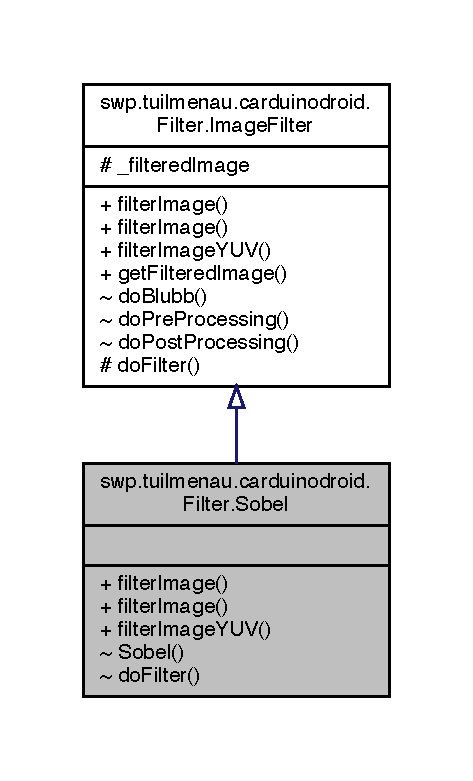
\includegraphics[width=227pt]{classswp_1_1tuilmenau_1_1carduinodroid_1_1_filter_1_1_sobel__inherit__graph}
\end{center}
\end{figure}


Collaboration diagram for swp.\+tuilmenau.\+carduinodroid.\+Filter.\+Sobel\+:
\nopagebreak
\begin{figure}[H]
\begin{center}
\leavevmode
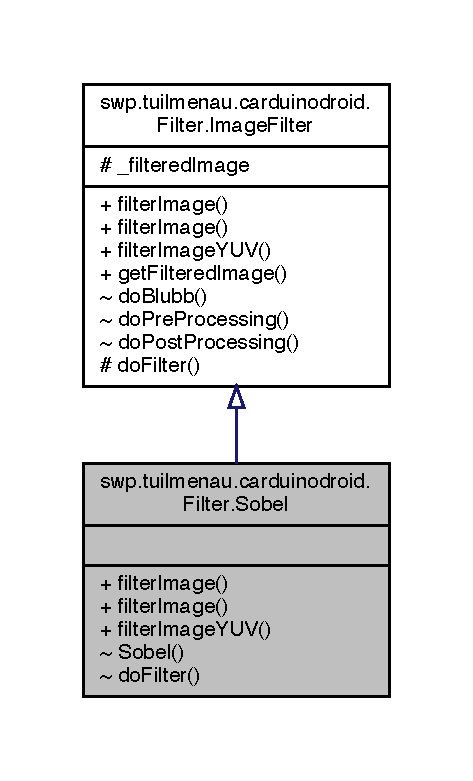
\includegraphics[width=227pt]{classswp_1_1tuilmenau_1_1carduinodroid_1_1_filter_1_1_sobel__coll__graph}
\end{center}
\end{figure}
\subsection*{Public Member Functions}
\begin{DoxyCompactItemize}
\item 
Bitmap \hyperlink{classswp_1_1tuilmenau_1_1carduinodroid_1_1_filter_1_1_sobel_ac5487d48e3b5bc2ee76f463ca088f31a}{filter\+Image} (byte\mbox{[}$\,$\mbox{]} f)
\item 
Bitmap \hyperlink{classswp_1_1tuilmenau_1_1carduinodroid_1_1_filter_1_1_sobel_ae7a8d5c6f0bd1b1e2db578bff09999c2}{filter\+Image} (byte\mbox{[}$\,$\mbox{]} f, int width, int height)
\item 
Yuv\+Image \hyperlink{classswp_1_1tuilmenau_1_1carduinodroid_1_1_filter_1_1_sobel_abdb3e40a11f50b00c36bbd817a9db5fd}{filter\+Image\+Y\+U\+V} (byte\mbox{[}$\,$\mbox{]} f, int width, int height)
\end{DoxyCompactItemize}
\subsection*{Additional Inherited Members}


\subsection{Member Function Documentation}
\hypertarget{classswp_1_1tuilmenau_1_1carduinodroid_1_1_filter_1_1_sobel_ac5487d48e3b5bc2ee76f463ca088f31a}{}\index{swp\+::tuilmenau\+::carduinodroid\+::\+Filter\+::\+Sobel@{swp\+::tuilmenau\+::carduinodroid\+::\+Filter\+::\+Sobel}!filter\+Image@{filter\+Image}}
\index{filter\+Image@{filter\+Image}!swp\+::tuilmenau\+::carduinodroid\+::\+Filter\+::\+Sobel@{swp\+::tuilmenau\+::carduinodroid\+::\+Filter\+::\+Sobel}}
\subsubsection[{filter\+Image}]{\setlength{\rightskip}{0pt plus 5cm}Bitmap swp.\+tuilmenau.\+carduinodroid.\+Filter.\+Sobel.\+filter\+Image (
\begin{DoxyParamCaption}
\item[{byte\mbox{[}$\,$\mbox{]}}]{f}
\end{DoxyParamCaption}
)}\label{classswp_1_1tuilmenau_1_1carduinodroid_1_1_filter_1_1_sobel_ac5487d48e3b5bc2ee76f463ca088f31a}
\hypertarget{classswp_1_1tuilmenau_1_1carduinodroid_1_1_filter_1_1_sobel_ae7a8d5c6f0bd1b1e2db578bff09999c2}{}\index{swp\+::tuilmenau\+::carduinodroid\+::\+Filter\+::\+Sobel@{swp\+::tuilmenau\+::carduinodroid\+::\+Filter\+::\+Sobel}!filter\+Image@{filter\+Image}}
\index{filter\+Image@{filter\+Image}!swp\+::tuilmenau\+::carduinodroid\+::\+Filter\+::\+Sobel@{swp\+::tuilmenau\+::carduinodroid\+::\+Filter\+::\+Sobel}}
\subsubsection[{filter\+Image}]{\setlength{\rightskip}{0pt plus 5cm}Bitmap swp.\+tuilmenau.\+carduinodroid.\+Filter.\+Sobel.\+filter\+Image (
\begin{DoxyParamCaption}
\item[{byte\mbox{[}$\,$\mbox{]}}]{f, }
\item[{int}]{width, }
\item[{int}]{height}
\end{DoxyParamCaption}
)}\label{classswp_1_1tuilmenau_1_1carduinodroid_1_1_filter_1_1_sobel_ae7a8d5c6f0bd1b1e2db578bff09999c2}
\hypertarget{classswp_1_1tuilmenau_1_1carduinodroid_1_1_filter_1_1_sobel_abdb3e40a11f50b00c36bbd817a9db5fd}{}\index{swp\+::tuilmenau\+::carduinodroid\+::\+Filter\+::\+Sobel@{swp\+::tuilmenau\+::carduinodroid\+::\+Filter\+::\+Sobel}!filter\+Image\+Y\+U\+V@{filter\+Image\+Y\+U\+V}}
\index{filter\+Image\+Y\+U\+V@{filter\+Image\+Y\+U\+V}!swp\+::tuilmenau\+::carduinodroid\+::\+Filter\+::\+Sobel@{swp\+::tuilmenau\+::carduinodroid\+::\+Filter\+::\+Sobel}}
\subsubsection[{filter\+Image\+Y\+U\+V}]{\setlength{\rightskip}{0pt plus 5cm}Yuv\+Image swp.\+tuilmenau.\+carduinodroid.\+Filter.\+Sobel.\+filter\+Image\+Y\+U\+V (
\begin{DoxyParamCaption}
\item[{byte\mbox{[}$\,$\mbox{]}}]{f, }
\item[{int}]{width, }
\item[{int}]{height}
\end{DoxyParamCaption}
)}\label{classswp_1_1tuilmenau_1_1carduinodroid_1_1_filter_1_1_sobel_abdb3e40a11f50b00c36bbd817a9db5fd}


The documentation for this class was generated from the following file\+:\begin{DoxyCompactItemize}
\item 
src/swp/tuilmenau/carduinodroid/\+Filter/\hyperlink{_sobel_8java}{Sobel.\+java}\end{DoxyCompactItemize}

\hypertarget{classswp_1_1tuilmenau_1_1carduinodroid_1_1controller_1_1_socket___controller}{}\section{swp.\+tuilmenau.\+carduinodroid.\+controller.\+Socket\+\_\+\+Controller Class Reference}
\label{classswp_1_1tuilmenau_1_1carduinodroid_1_1controller_1_1_socket___controller}\index{swp.\+tuilmenau.\+carduinodroid.\+controller.\+Socket\+\_\+\+Controller@{swp.\+tuilmenau.\+carduinodroid.\+controller.\+Socket\+\_\+\+Controller}}


Inheritance diagram for swp.\+tuilmenau.\+carduinodroid.\+controller.\+Socket\+\_\+\+Controller\+:
\nopagebreak
\begin{figure}[H]
\begin{center}
\leavevmode
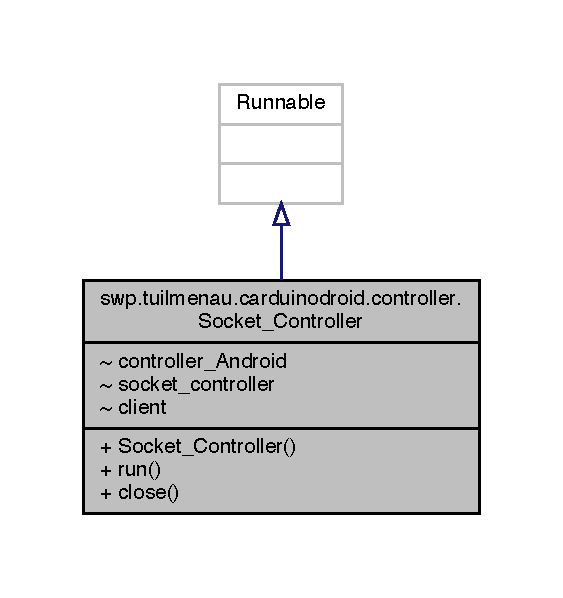
\includegraphics[width=270pt]{classswp_1_1tuilmenau_1_1carduinodroid_1_1controller_1_1_socket___controller__inherit__graph}
\end{center}
\end{figure}


Collaboration diagram for swp.\+tuilmenau.\+carduinodroid.\+controller.\+Socket\+\_\+\+Controller\+:
\nopagebreak
\begin{figure}[H]
\begin{center}
\leavevmode
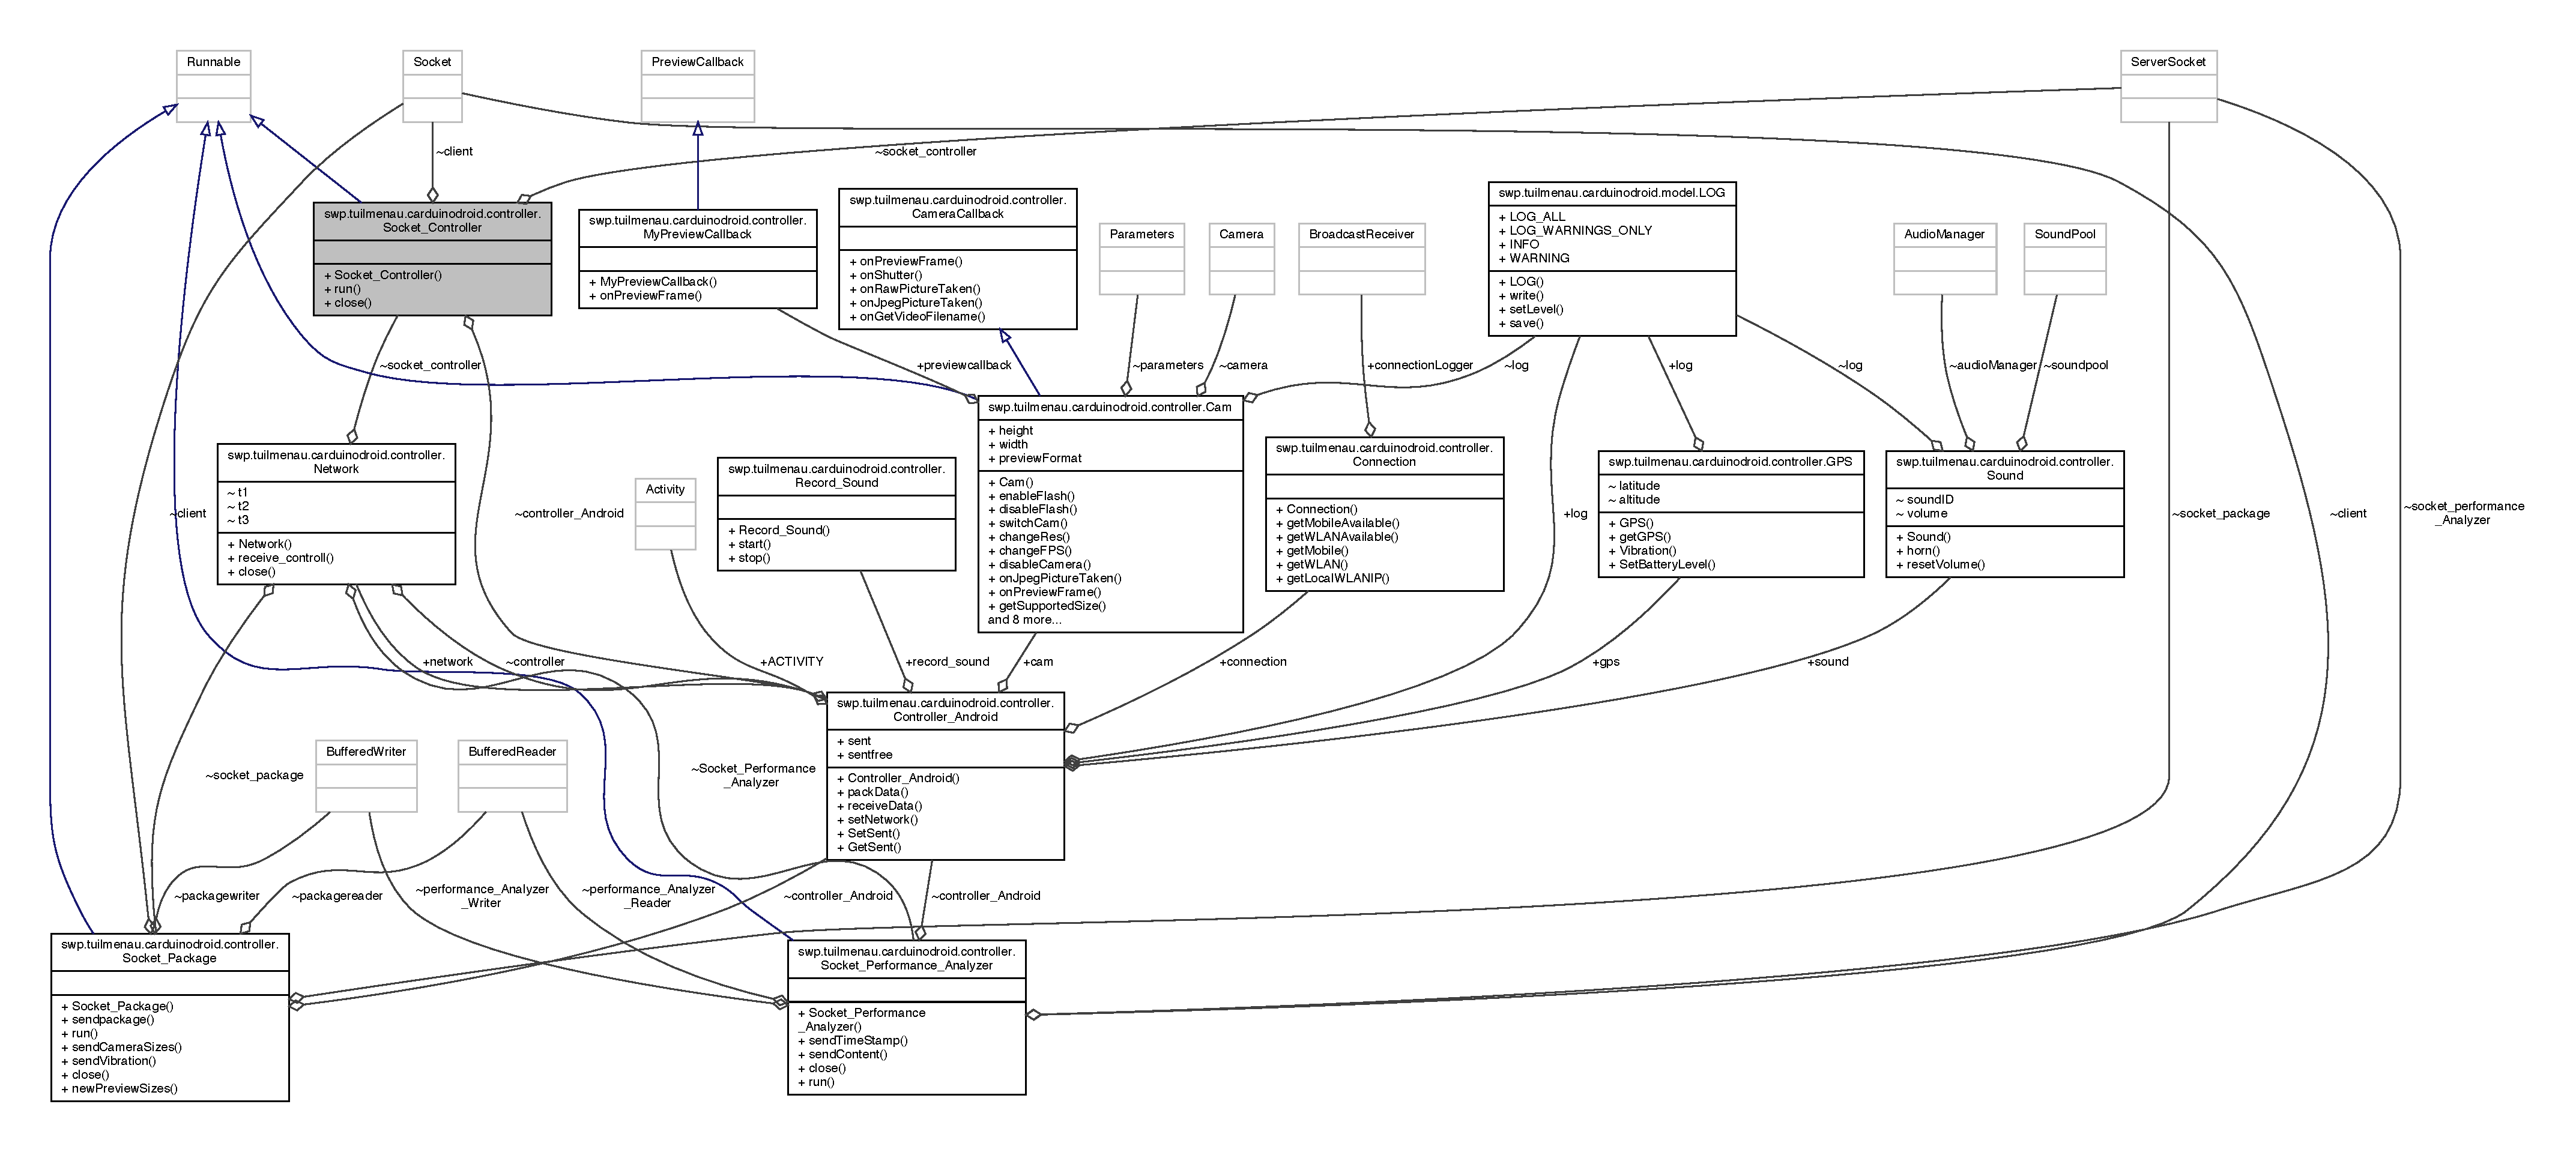
\includegraphics[width=350pt]{classswp_1_1tuilmenau_1_1carduinodroid_1_1controller_1_1_socket___controller__coll__graph}
\end{center}
\end{figure}
\subsection*{Public Member Functions}
\begin{DoxyCompactItemize}
\item 
\hyperlink{classswp_1_1tuilmenau_1_1carduinodroid_1_1controller_1_1_socket___controller_ab69baec0ffe38654dade8dff77c3767e}{Socket\+\_\+\+Controller} (\hyperlink{classswp_1_1tuilmenau_1_1carduinodroid_1_1controller_1_1_controller___android}{Controller\+\_\+\+Android} n\+\_\+controller\+\_\+\+Android)
\item 
void \hyperlink{classswp_1_1tuilmenau_1_1carduinodroid_1_1controller_1_1_socket___controller_a490674a59c3992603e27ef75821e61d6}{run} ()
\item 
void \hyperlink{classswp_1_1tuilmenau_1_1carduinodroid_1_1controller_1_1_socket___controller_a08ccd8feecfa1c15480137de90e24d23}{close} ()
\end{DoxyCompactItemize}


\subsection{Detailed Description}
This class is used for receiving data from the pc to control the application

\begin{DoxyAuthor}{Author}
Robin 
\end{DoxyAuthor}


\subsection{Constructor \& Destructor Documentation}
\hypertarget{classswp_1_1tuilmenau_1_1carduinodroid_1_1controller_1_1_socket___controller_ab69baec0ffe38654dade8dff77c3767e}{}\index{swp\+::tuilmenau\+::carduinodroid\+::controller\+::\+Socket\+\_\+\+Controller@{swp\+::tuilmenau\+::carduinodroid\+::controller\+::\+Socket\+\_\+\+Controller}!Socket\+\_\+\+Controller@{Socket\+\_\+\+Controller}}
\index{Socket\+\_\+\+Controller@{Socket\+\_\+\+Controller}!swp\+::tuilmenau\+::carduinodroid\+::controller\+::\+Socket\+\_\+\+Controller@{swp\+::tuilmenau\+::carduinodroid\+::controller\+::\+Socket\+\_\+\+Controller}}
\subsubsection[{Socket\+\_\+\+Controller}]{\setlength{\rightskip}{0pt plus 5cm}swp.\+tuilmenau.\+carduinodroid.\+controller.\+Socket\+\_\+\+Controller.\+Socket\+\_\+\+Controller (
\begin{DoxyParamCaption}
\item[{{\bf Controller\+\_\+\+Android}}]{n\+\_\+controller\+\_\+\+Android}
\end{DoxyParamCaption}
)}\label{classswp_1_1tuilmenau_1_1carduinodroid_1_1controller_1_1_socket___controller_ab69baec0ffe38654dade8dff77c3767e}
The constructor of the \hyperlink{classswp_1_1tuilmenau_1_1carduinodroid_1_1controller_1_1_socket___controller}{Socket\+\_\+\+Controller}


\begin{DoxyParams}{Parameters}
{\em n\+\_\+controller\+\_\+\+Android} & \\
\hline
\end{DoxyParams}


\subsection{Member Function Documentation}
\hypertarget{classswp_1_1tuilmenau_1_1carduinodroid_1_1controller_1_1_socket___controller_a08ccd8feecfa1c15480137de90e24d23}{}\index{swp\+::tuilmenau\+::carduinodroid\+::controller\+::\+Socket\+\_\+\+Controller@{swp\+::tuilmenau\+::carduinodroid\+::controller\+::\+Socket\+\_\+\+Controller}!close@{close}}
\index{close@{close}!swp\+::tuilmenau\+::carduinodroid\+::controller\+::\+Socket\+\_\+\+Controller@{swp\+::tuilmenau\+::carduinodroid\+::controller\+::\+Socket\+\_\+\+Controller}}
\subsubsection[{close}]{\setlength{\rightskip}{0pt plus 5cm}void swp.\+tuilmenau.\+carduinodroid.\+controller.\+Socket\+\_\+\+Controller.\+close (
\begin{DoxyParamCaption}
{}
\end{DoxyParamCaption}
)}\label{classswp_1_1tuilmenau_1_1carduinodroid_1_1controller_1_1_socket___controller_a08ccd8feecfa1c15480137de90e24d23}


Here is the caller graph for this function\+:
\nopagebreak
\begin{figure}[H]
\begin{center}
\leavevmode
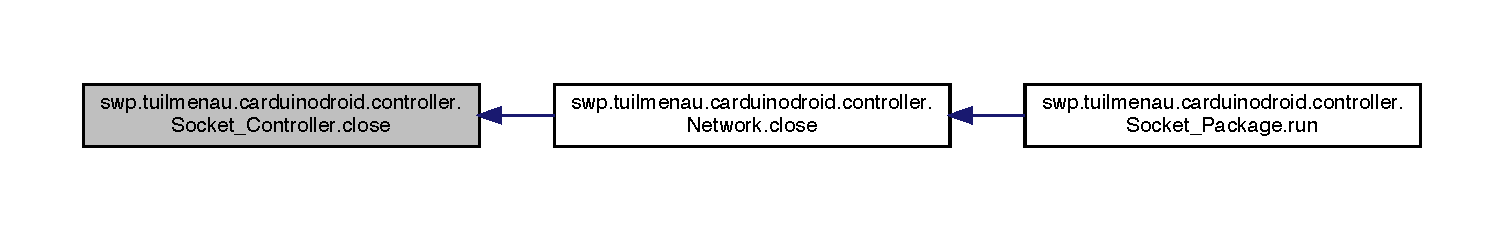
\includegraphics[width=350pt]{classswp_1_1tuilmenau_1_1carduinodroid_1_1controller_1_1_socket___controller_a08ccd8feecfa1c15480137de90e24d23_icgraph}
\end{center}
\end{figure}


\hypertarget{classswp_1_1tuilmenau_1_1carduinodroid_1_1controller_1_1_socket___controller_a490674a59c3992603e27ef75821e61d6}{}\index{swp\+::tuilmenau\+::carduinodroid\+::controller\+::\+Socket\+\_\+\+Controller@{swp\+::tuilmenau\+::carduinodroid\+::controller\+::\+Socket\+\_\+\+Controller}!run@{run}}
\index{run@{run}!swp\+::tuilmenau\+::carduinodroid\+::controller\+::\+Socket\+\_\+\+Controller@{swp\+::tuilmenau\+::carduinodroid\+::controller\+::\+Socket\+\_\+\+Controller}}
\subsubsection[{run}]{\setlength{\rightskip}{0pt plus 5cm}void swp.\+tuilmenau.\+carduinodroid.\+controller.\+Socket\+\_\+\+Controller.\+run (
\begin{DoxyParamCaption}
{}
\end{DoxyParamCaption}
)}\label{classswp_1_1tuilmenau_1_1carduinodroid_1_1controller_1_1_socket___controller_a490674a59c3992603e27ef75821e61d6}


Here is the call graph for this function\+:
\nopagebreak
\begin{figure}[H]
\begin{center}
\leavevmode
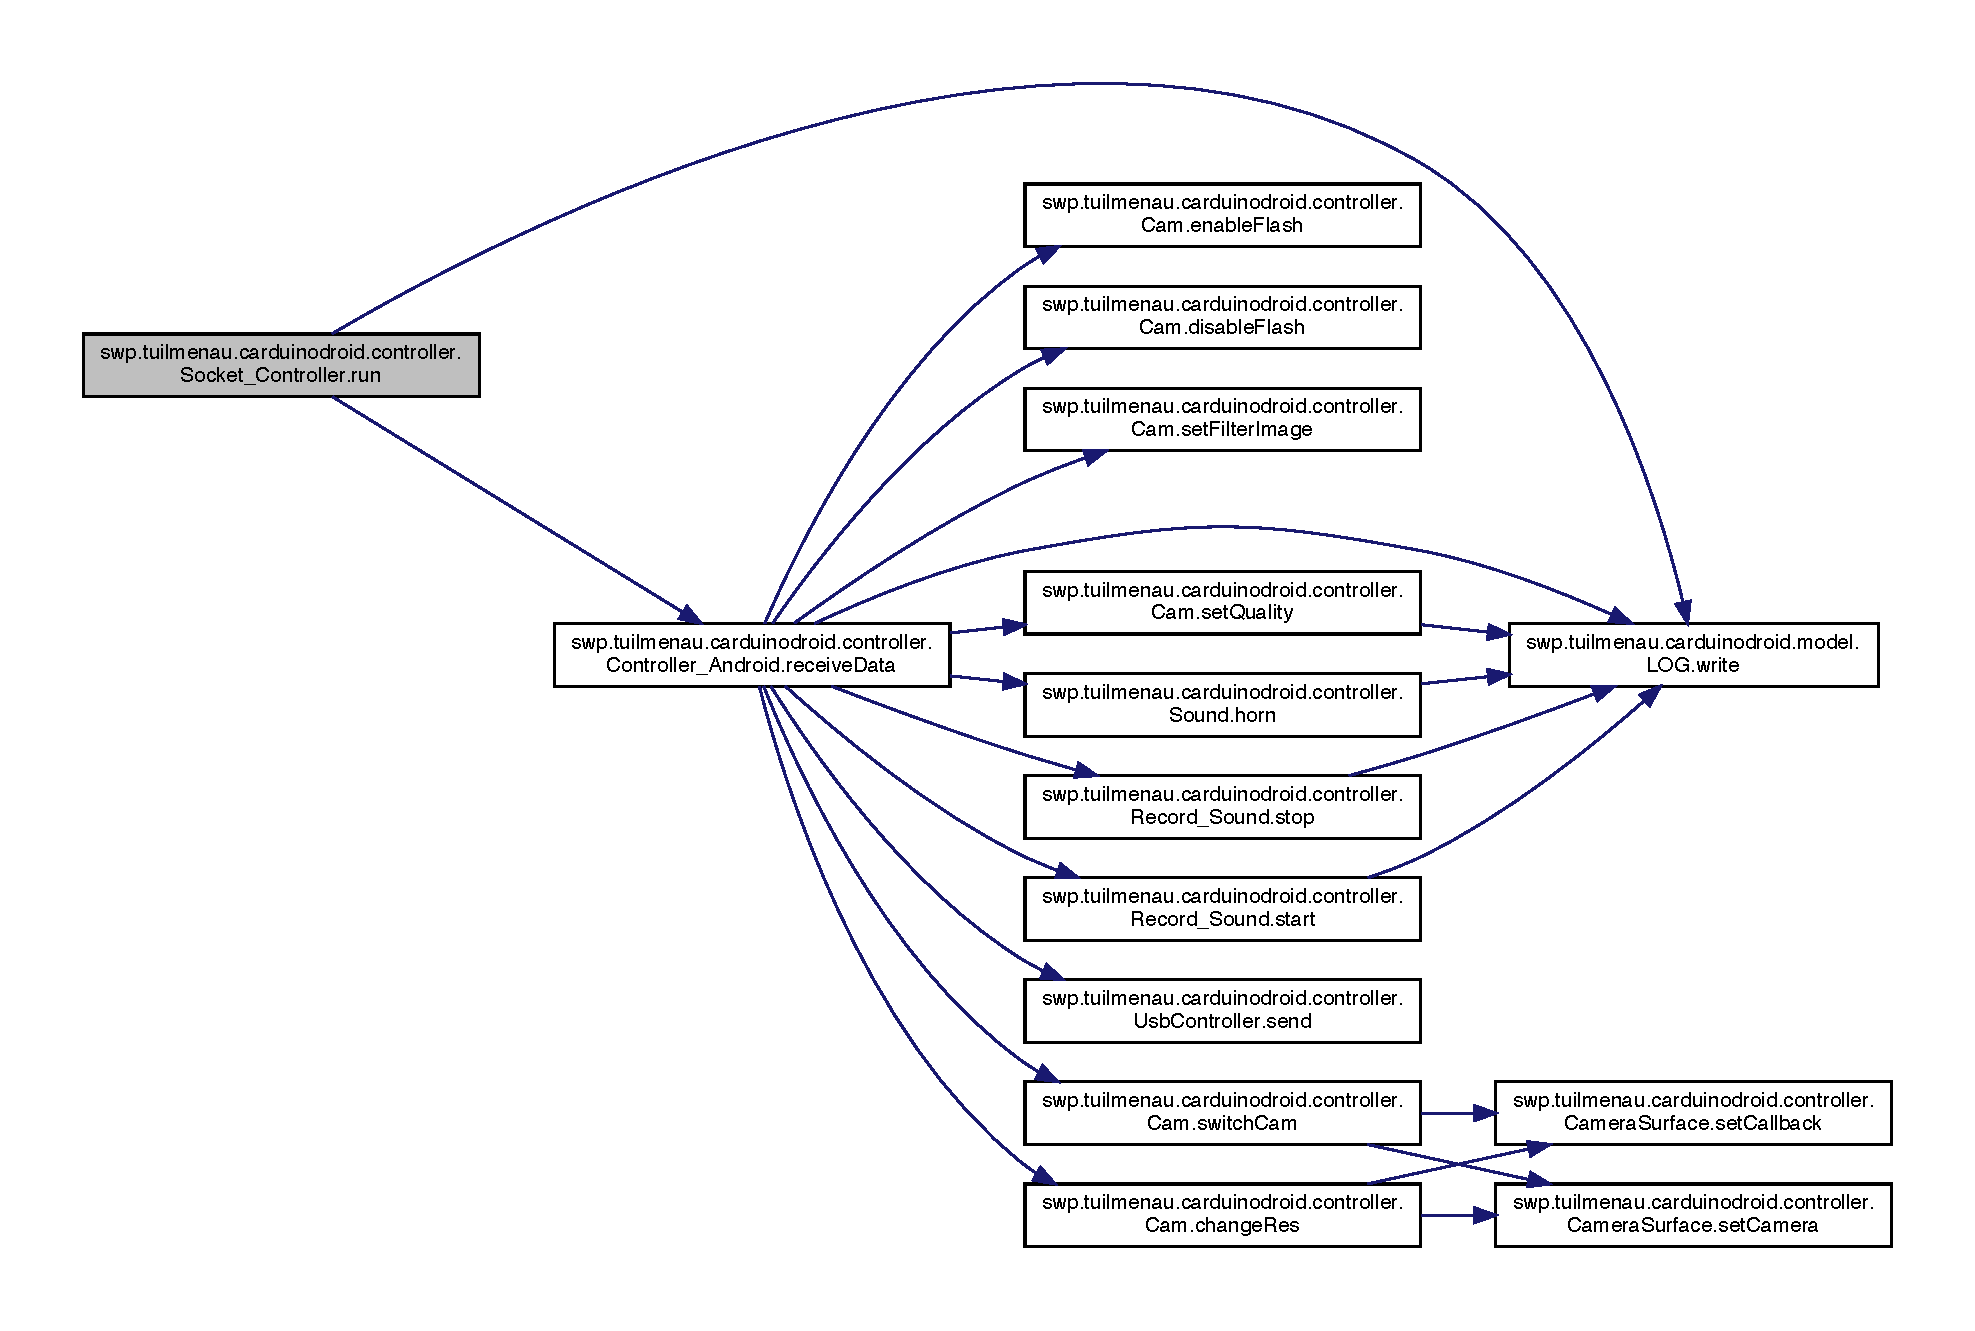
\includegraphics[width=350pt]{classswp_1_1tuilmenau_1_1carduinodroid_1_1controller_1_1_socket___controller_a490674a59c3992603e27ef75821e61d6_cgraph}
\end{center}
\end{figure}




The documentation for this class was generated from the following file\+:\begin{DoxyCompactItemize}
\item 
src/swp/tuilmenau/carduinodroid/controller/\hyperlink{_socket___controller_8java}{Socket\+\_\+\+Controller.\+java}\end{DoxyCompactItemize}

\hypertarget{classswp_1_1tuilmenau_1_1carduinodroid_1_1controller_1_1_socket___package}{}\section{swp.\+tuilmenau.\+carduinodroid.\+controller.\+Socket\+\_\+\+Package Class Reference}
\label{classswp_1_1tuilmenau_1_1carduinodroid_1_1controller_1_1_socket___package}\index{swp.\+tuilmenau.\+carduinodroid.\+controller.\+Socket\+\_\+\+Package@{swp.\+tuilmenau.\+carduinodroid.\+controller.\+Socket\+\_\+\+Package}}


Inheritance diagram for swp.\+tuilmenau.\+carduinodroid.\+controller.\+Socket\+\_\+\+Package\+:
\nopagebreak
\begin{figure}[H]
\begin{center}
\leavevmode
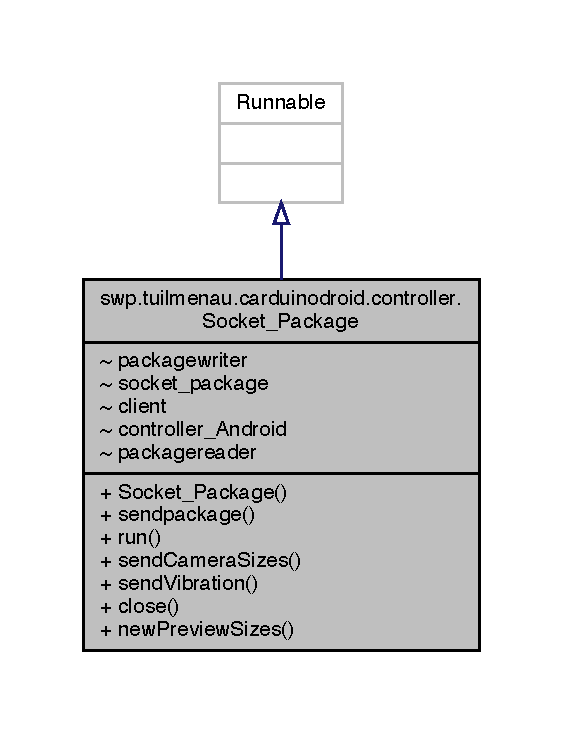
\includegraphics[width=270pt]{classswp_1_1tuilmenau_1_1carduinodroid_1_1controller_1_1_socket___package__inherit__graph}
\end{center}
\end{figure}


Collaboration diagram for swp.\+tuilmenau.\+carduinodroid.\+controller.\+Socket\+\_\+\+Package\+:
\nopagebreak
\begin{figure}[H]
\begin{center}
\leavevmode
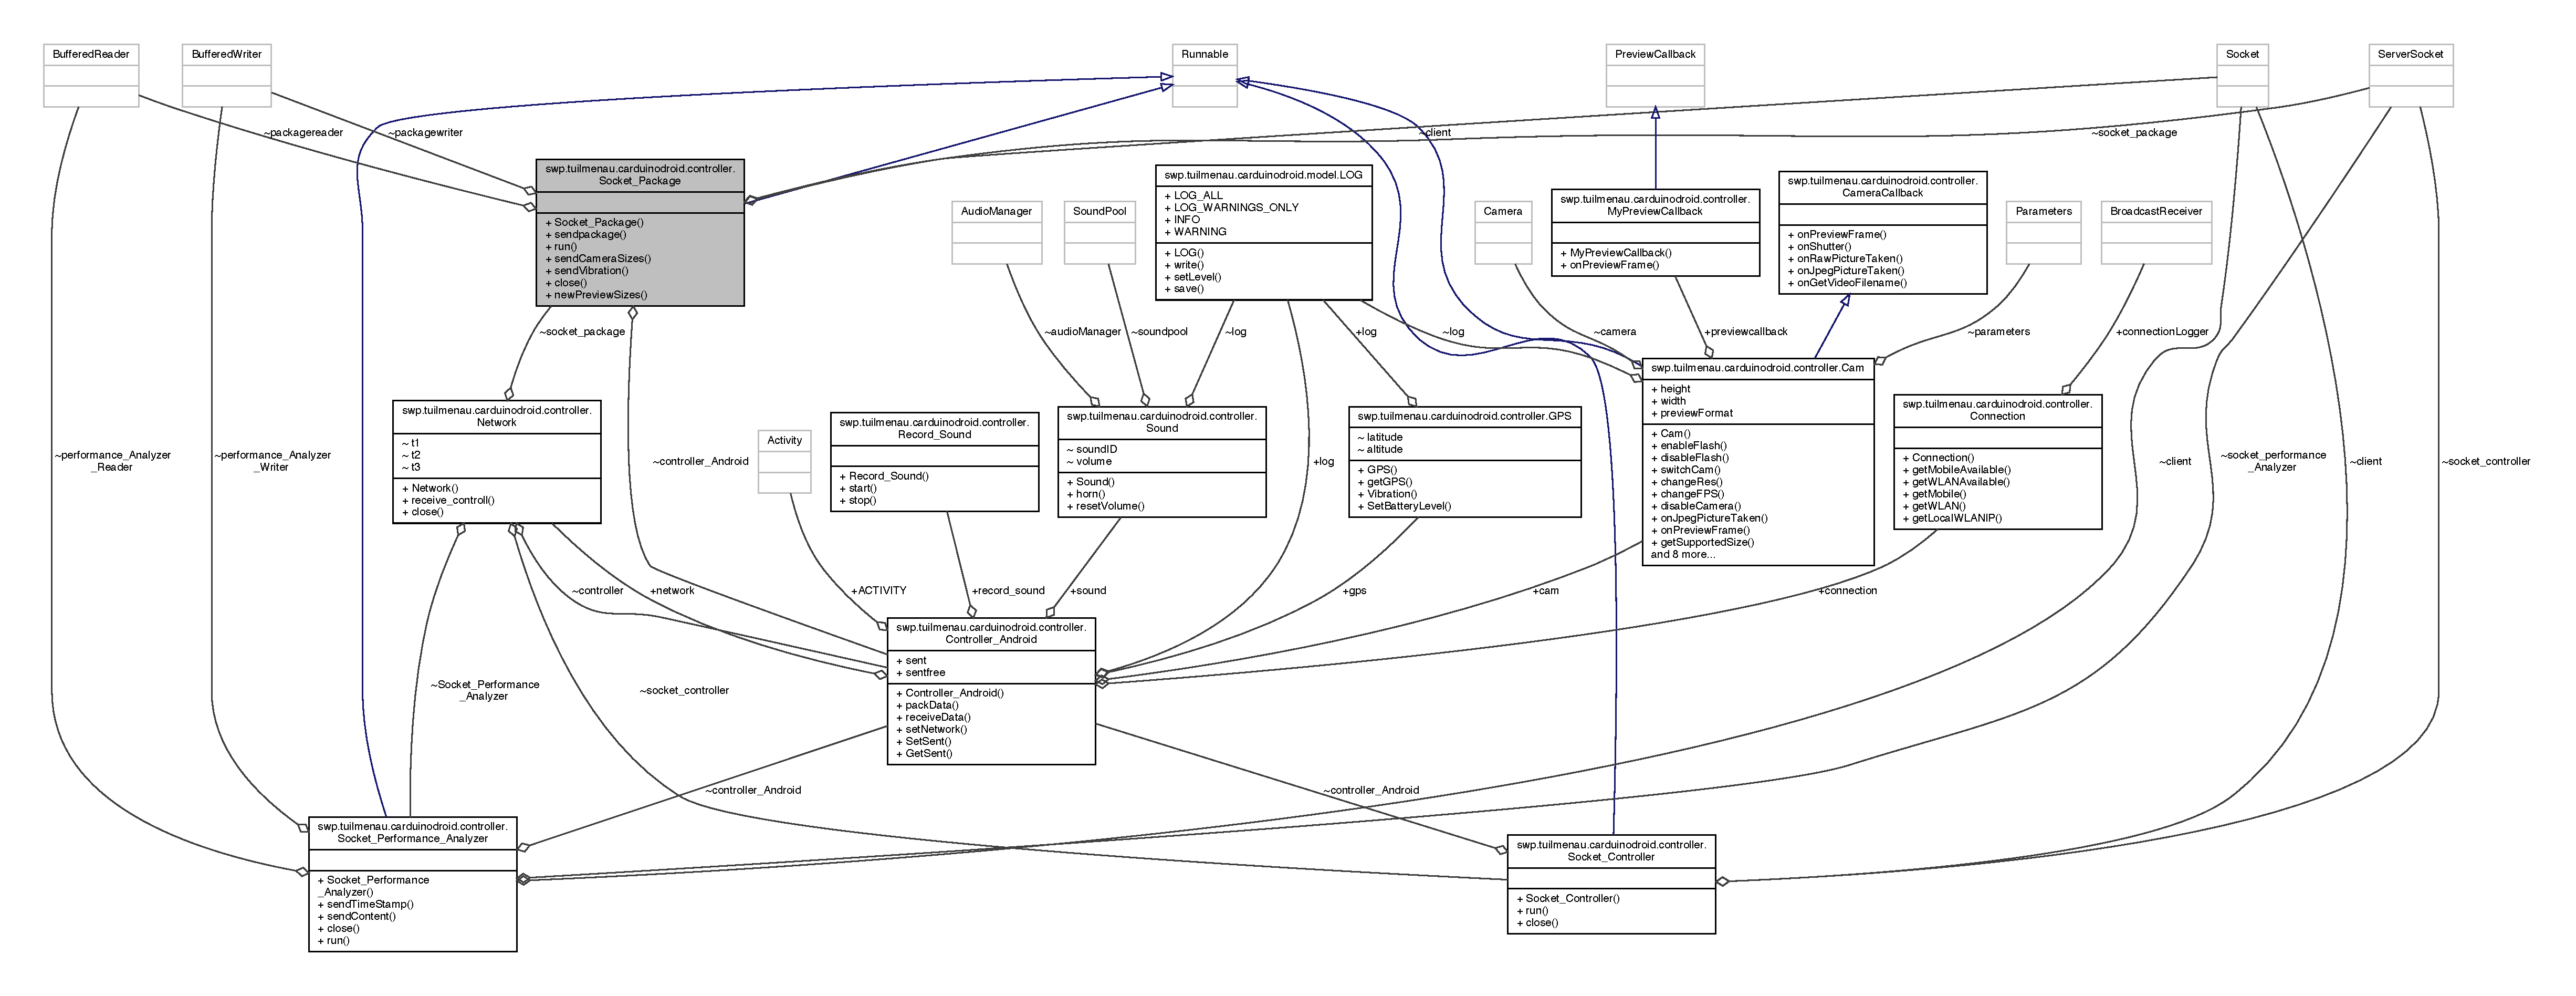
\includegraphics[width=350pt]{classswp_1_1tuilmenau_1_1carduinodroid_1_1controller_1_1_socket___package__coll__graph}
\end{center}
\end{figure}
\subsection*{Public Member Functions}
\begin{DoxyCompactItemize}
\item 
\hyperlink{classswp_1_1tuilmenau_1_1carduinodroid_1_1controller_1_1_socket___package_aa4bb757cfbf01a6dd21d114690131248}{Socket\+\_\+\+Package} (\hyperlink{classswp_1_1tuilmenau_1_1carduinodroid_1_1controller_1_1_controller___android}{Controller\+\_\+\+Android} n\+\_\+controller\+\_\+\+Android, \hyperlink{classswp_1_1tuilmenau_1_1carduinodroid_1_1controller_1_1_network}{Network} nnetwork)
\item 
boolean \hyperlink{classswp_1_1tuilmenau_1_1carduinodroid_1_1controller_1_1_socket___package_af1f59a4d10ed02a41fdbfbe189d51922}{sendpackage} (String infopackage)
\item 
void \hyperlink{classswp_1_1tuilmenau_1_1carduinodroid_1_1controller_1_1_socket___package_a5ac59e8b14090f0669452997e1d55a09}{run} ()
\item 
void \hyperlink{classswp_1_1tuilmenau_1_1carduinodroid_1_1controller_1_1_socket___package_a3e8a8bb73c0297f4589d74cb622689d4}{send\+Camera\+Sizes} ()
\item 
void \hyperlink{classswp_1_1tuilmenau_1_1carduinodroid_1_1controller_1_1_socket___package_ac94eadb1cae5fe5ed772c92c36ff81b6}{send\+Vibration} ()
\item 
void \hyperlink{classswp_1_1tuilmenau_1_1carduinodroid_1_1controller_1_1_socket___package_aa1379b7f52f3773259cf1c6fb08fb2a9}{close} ()
\item 
void \hyperlink{classswp_1_1tuilmenau_1_1carduinodroid_1_1controller_1_1_socket___package_a37c276fcdbfcbbe5f608531c255d3b00}{new\+Preview\+Sizes} ()
\end{DoxyCompactItemize}


\subsection{Detailed Description}
This class is used to send information to the P\+C

\begin{DoxyAuthor}{Author}
Robin 
\end{DoxyAuthor}


\subsection{Constructor \& Destructor Documentation}
\hypertarget{classswp_1_1tuilmenau_1_1carduinodroid_1_1controller_1_1_socket___package_aa4bb757cfbf01a6dd21d114690131248}{}\index{swp\+::tuilmenau\+::carduinodroid\+::controller\+::\+Socket\+\_\+\+Package@{swp\+::tuilmenau\+::carduinodroid\+::controller\+::\+Socket\+\_\+\+Package}!Socket\+\_\+\+Package@{Socket\+\_\+\+Package}}
\index{Socket\+\_\+\+Package@{Socket\+\_\+\+Package}!swp\+::tuilmenau\+::carduinodroid\+::controller\+::\+Socket\+\_\+\+Package@{swp\+::tuilmenau\+::carduinodroid\+::controller\+::\+Socket\+\_\+\+Package}}
\subsubsection[{Socket\+\_\+\+Package}]{\setlength{\rightskip}{0pt plus 5cm}swp.\+tuilmenau.\+carduinodroid.\+controller.\+Socket\+\_\+\+Package.\+Socket\+\_\+\+Package (
\begin{DoxyParamCaption}
\item[{{\bf Controller\+\_\+\+Android}}]{n\+\_\+controller\+\_\+\+Android, }
\item[{{\bf Network}}]{nnetwork}
\end{DoxyParamCaption}
)}\label{classswp_1_1tuilmenau_1_1carduinodroid_1_1controller_1_1_socket___package_aa4bb757cfbf01a6dd21d114690131248}
The constructor


\begin{DoxyParams}{Parameters}
{\em n\+\_\+controller\+\_\+\+Android} & \\
\hline
\end{DoxyParams}


\subsection{Member Function Documentation}
\hypertarget{classswp_1_1tuilmenau_1_1carduinodroid_1_1controller_1_1_socket___package_aa1379b7f52f3773259cf1c6fb08fb2a9}{}\index{swp\+::tuilmenau\+::carduinodroid\+::controller\+::\+Socket\+\_\+\+Package@{swp\+::tuilmenau\+::carduinodroid\+::controller\+::\+Socket\+\_\+\+Package}!close@{close}}
\index{close@{close}!swp\+::tuilmenau\+::carduinodroid\+::controller\+::\+Socket\+\_\+\+Package@{swp\+::tuilmenau\+::carduinodroid\+::controller\+::\+Socket\+\_\+\+Package}}
\subsubsection[{close}]{\setlength{\rightskip}{0pt plus 5cm}void swp.\+tuilmenau.\+carduinodroid.\+controller.\+Socket\+\_\+\+Package.\+close (
\begin{DoxyParamCaption}
{}
\end{DoxyParamCaption}
)}\label{classswp_1_1tuilmenau_1_1carduinodroid_1_1controller_1_1_socket___package_aa1379b7f52f3773259cf1c6fb08fb2a9}


Here is the caller graph for this function\+:
\nopagebreak
\begin{figure}[H]
\begin{center}
\leavevmode
\includegraphics[width=350pt]{classswp_1_1tuilmenau_1_1carduinodroid_1_1controller_1_1_socket___package_aa1379b7f52f3773259cf1c6fb08fb2a9_icgraph}
\end{center}
\end{figure}


\hypertarget{classswp_1_1tuilmenau_1_1carduinodroid_1_1controller_1_1_socket___package_a37c276fcdbfcbbe5f608531c255d3b00}{}\index{swp\+::tuilmenau\+::carduinodroid\+::controller\+::\+Socket\+\_\+\+Package@{swp\+::tuilmenau\+::carduinodroid\+::controller\+::\+Socket\+\_\+\+Package}!new\+Preview\+Sizes@{new\+Preview\+Sizes}}
\index{new\+Preview\+Sizes@{new\+Preview\+Sizes}!swp\+::tuilmenau\+::carduinodroid\+::controller\+::\+Socket\+\_\+\+Package@{swp\+::tuilmenau\+::carduinodroid\+::controller\+::\+Socket\+\_\+\+Package}}
\subsubsection[{new\+Preview\+Sizes}]{\setlength{\rightskip}{0pt plus 5cm}void swp.\+tuilmenau.\+carduinodroid.\+controller.\+Socket\+\_\+\+Package.\+new\+Preview\+Sizes (
\begin{DoxyParamCaption}
{}
\end{DoxyParamCaption}
)}\label{classswp_1_1tuilmenau_1_1carduinodroid_1_1controller_1_1_socket___package_a37c276fcdbfcbbe5f608531c255d3b00}
\hypertarget{classswp_1_1tuilmenau_1_1carduinodroid_1_1controller_1_1_socket___package_a5ac59e8b14090f0669452997e1d55a09}{}\index{swp\+::tuilmenau\+::carduinodroid\+::controller\+::\+Socket\+\_\+\+Package@{swp\+::tuilmenau\+::carduinodroid\+::controller\+::\+Socket\+\_\+\+Package}!run@{run}}
\index{run@{run}!swp\+::tuilmenau\+::carduinodroid\+::controller\+::\+Socket\+\_\+\+Package@{swp\+::tuilmenau\+::carduinodroid\+::controller\+::\+Socket\+\_\+\+Package}}
\subsubsection[{run}]{\setlength{\rightskip}{0pt plus 5cm}void swp.\+tuilmenau.\+carduinodroid.\+controller.\+Socket\+\_\+\+Package.\+run (
\begin{DoxyParamCaption}
{}
\end{DoxyParamCaption}
)}\label{classswp_1_1tuilmenau_1_1carduinodroid_1_1controller_1_1_socket___package_a5ac59e8b14090f0669452997e1d55a09}


Here is the call graph for this function\+:
\nopagebreak
\begin{figure}[H]
\begin{center}
\leavevmode
\includegraphics[width=350pt]{classswp_1_1tuilmenau_1_1carduinodroid_1_1controller_1_1_socket___package_a5ac59e8b14090f0669452997e1d55a09_cgraph}
\end{center}
\end{figure}


\hypertarget{classswp_1_1tuilmenau_1_1carduinodroid_1_1controller_1_1_socket___package_a3e8a8bb73c0297f4589d74cb622689d4}{}\index{swp\+::tuilmenau\+::carduinodroid\+::controller\+::\+Socket\+\_\+\+Package@{swp\+::tuilmenau\+::carduinodroid\+::controller\+::\+Socket\+\_\+\+Package}!send\+Camera\+Sizes@{send\+Camera\+Sizes}}
\index{send\+Camera\+Sizes@{send\+Camera\+Sizes}!swp\+::tuilmenau\+::carduinodroid\+::controller\+::\+Socket\+\_\+\+Package@{swp\+::tuilmenau\+::carduinodroid\+::controller\+::\+Socket\+\_\+\+Package}}
\subsubsection[{send\+Camera\+Sizes}]{\setlength{\rightskip}{0pt plus 5cm}void swp.\+tuilmenau.\+carduinodroid.\+controller.\+Socket\+\_\+\+Package.\+send\+Camera\+Sizes (
\begin{DoxyParamCaption}
{}
\end{DoxyParamCaption}
)}\label{classswp_1_1tuilmenau_1_1carduinodroid_1_1controller_1_1_socket___package_a3e8a8bb73c0297f4589d74cb622689d4}


Here is the call graph for this function\+:
\nopagebreak
\begin{figure}[H]
\begin{center}
\leavevmode
\includegraphics[width=350pt]{classswp_1_1tuilmenau_1_1carduinodroid_1_1controller_1_1_socket___package_a3e8a8bb73c0297f4589d74cb622689d4_cgraph}
\end{center}
\end{figure}




Here is the caller graph for this function\+:
\nopagebreak
\begin{figure}[H]
\begin{center}
\leavevmode
\includegraphics[width=350pt]{classswp_1_1tuilmenau_1_1carduinodroid_1_1controller_1_1_socket___package_a3e8a8bb73c0297f4589d74cb622689d4_icgraph}
\end{center}
\end{figure}


\hypertarget{classswp_1_1tuilmenau_1_1carduinodroid_1_1controller_1_1_socket___package_af1f59a4d10ed02a41fdbfbe189d51922}{}\index{swp\+::tuilmenau\+::carduinodroid\+::controller\+::\+Socket\+\_\+\+Package@{swp\+::tuilmenau\+::carduinodroid\+::controller\+::\+Socket\+\_\+\+Package}!sendpackage@{sendpackage}}
\index{sendpackage@{sendpackage}!swp\+::tuilmenau\+::carduinodroid\+::controller\+::\+Socket\+\_\+\+Package@{swp\+::tuilmenau\+::carduinodroid\+::controller\+::\+Socket\+\_\+\+Package}}
\subsubsection[{sendpackage}]{\setlength{\rightskip}{0pt plus 5cm}boolean swp.\+tuilmenau.\+carduinodroid.\+controller.\+Socket\+\_\+\+Package.\+sendpackage (
\begin{DoxyParamCaption}
\item[{String}]{infopackage}
\end{DoxyParamCaption}
)}\label{classswp_1_1tuilmenau_1_1carduinodroid_1_1controller_1_1_socket___package_af1f59a4d10ed02a41fdbfbe189d51922}
Sends the information package to the socket


\begin{DoxyParams}{Parameters}
{\em infopackage} & The information \\
\hline
\end{DoxyParams}
\begin{DoxyReturn}{Returns}
true if successful 
\end{DoxyReturn}


Here is the caller graph for this function\+:
\nopagebreak
\begin{figure}[H]
\begin{center}
\leavevmode
\includegraphics[width=350pt]{classswp_1_1tuilmenau_1_1carduinodroid_1_1controller_1_1_socket___package_af1f59a4d10ed02a41fdbfbe189d51922_icgraph}
\end{center}
\end{figure}


\hypertarget{classswp_1_1tuilmenau_1_1carduinodroid_1_1controller_1_1_socket___package_ac94eadb1cae5fe5ed772c92c36ff81b6}{}\index{swp\+::tuilmenau\+::carduinodroid\+::controller\+::\+Socket\+\_\+\+Package@{swp\+::tuilmenau\+::carduinodroid\+::controller\+::\+Socket\+\_\+\+Package}!send\+Vibration@{send\+Vibration}}
\index{send\+Vibration@{send\+Vibration}!swp\+::tuilmenau\+::carduinodroid\+::controller\+::\+Socket\+\_\+\+Package@{swp\+::tuilmenau\+::carduinodroid\+::controller\+::\+Socket\+\_\+\+Package}}
\subsubsection[{send\+Vibration}]{\setlength{\rightskip}{0pt plus 5cm}void swp.\+tuilmenau.\+carduinodroid.\+controller.\+Socket\+\_\+\+Package.\+send\+Vibration (
\begin{DoxyParamCaption}
{}
\end{DoxyParamCaption}
)}\label{classswp_1_1tuilmenau_1_1carduinodroid_1_1controller_1_1_socket___package_ac94eadb1cae5fe5ed772c92c36ff81b6}


Here is the call graph for this function\+:
\nopagebreak
\begin{figure}[H]
\begin{center}
\leavevmode
\includegraphics[width=350pt]{classswp_1_1tuilmenau_1_1carduinodroid_1_1controller_1_1_socket___package_ac94eadb1cae5fe5ed772c92c36ff81b6_cgraph}
\end{center}
\end{figure}




Here is the caller graph for this function\+:
\nopagebreak
\begin{figure}[H]
\begin{center}
\leavevmode
\includegraphics[width=350pt]{classswp_1_1tuilmenau_1_1carduinodroid_1_1controller_1_1_socket___package_ac94eadb1cae5fe5ed772c92c36ff81b6_icgraph}
\end{center}
\end{figure}




The documentation for this class was generated from the following file\+:\begin{DoxyCompactItemize}
\item 
src/swp/tuilmenau/carduinodroid/controller/\hyperlink{_socket___package_8java}{Socket\+\_\+\+Package.\+java}\end{DoxyCompactItemize}

\hypertarget{classswp_1_1tuilmenau_1_1carduinodroid_1_1controller_1_1_socket___performance___analyzer}{}\section{swp.\+tuilmenau.\+carduinodroid.\+controller.\+Socket\+\_\+\+Performance\+\_\+\+Analyzer Class Reference}
\label{classswp_1_1tuilmenau_1_1carduinodroid_1_1controller_1_1_socket___performance___analyzer}\index{swp.\+tuilmenau.\+carduinodroid.\+controller.\+Socket\+\_\+\+Performance\+\_\+\+Analyzer@{swp.\+tuilmenau.\+carduinodroid.\+controller.\+Socket\+\_\+\+Performance\+\_\+\+Analyzer}}


Inheritance diagram for swp.\+tuilmenau.\+carduinodroid.\+controller.\+Socket\+\_\+\+Performance\+\_\+\+Analyzer\+:
\nopagebreak
\begin{figure}[H]
\begin{center}
\leavevmode
\includegraphics[width=270pt]{classswp_1_1tuilmenau_1_1carduinodroid_1_1controller_1_1_socket___performance___analyzer__inherit__graph}
\end{center}
\end{figure}


Collaboration diagram for swp.\+tuilmenau.\+carduinodroid.\+controller.\+Socket\+\_\+\+Performance\+\_\+\+Analyzer\+:
\nopagebreak
\begin{figure}[H]
\begin{center}
\leavevmode
\includegraphics[width=350pt]{classswp_1_1tuilmenau_1_1carduinodroid_1_1controller_1_1_socket___performance___analyzer__coll__graph}
\end{center}
\end{figure}
\subsection*{Public Member Functions}
\begin{DoxyCompactItemize}
\item 
\hyperlink{classswp_1_1tuilmenau_1_1carduinodroid_1_1controller_1_1_socket___performance___analyzer_ad8b07b2fa1ef425a0799534eac638e2c}{Socket\+\_\+\+Performance\+\_\+\+Analyzer} (\hyperlink{classswp_1_1tuilmenau_1_1carduinodroid_1_1controller_1_1_controller___android}{Controller\+\_\+\+Android} n\+\_\+controller\+\_\+\+Android, \hyperlink{classswp_1_1tuilmenau_1_1carduinodroid_1_1controller_1_1_network}{Network} nnetwork)
\item 
boolean \hyperlink{classswp_1_1tuilmenau_1_1carduinodroid_1_1controller_1_1_socket___performance___analyzer_a7cb9ff89df5010aada87f12106ae780f}{send\+Time\+Stamp} ()
\item 
boolean \hyperlink{classswp_1_1tuilmenau_1_1carduinodroid_1_1controller_1_1_socket___performance___analyzer_a978fc027e3ba8daba45d97ec3b4e01a7}{send\+Content} (String content)
\item 
void \hyperlink{classswp_1_1tuilmenau_1_1carduinodroid_1_1controller_1_1_socket___performance___analyzer_a268ebda216316321db775f2b7dc3459b}{close} ()
\item 
void \hyperlink{classswp_1_1tuilmenau_1_1carduinodroid_1_1controller_1_1_socket___performance___analyzer_a53e5cd2c2f619c2d651b7d9dfea11e7a}{run} ()
\end{DoxyCompactItemize}


\subsection{Constructor \& Destructor Documentation}
\hypertarget{classswp_1_1tuilmenau_1_1carduinodroid_1_1controller_1_1_socket___performance___analyzer_ad8b07b2fa1ef425a0799534eac638e2c}{}\index{swp\+::tuilmenau\+::carduinodroid\+::controller\+::\+Socket\+\_\+\+Performance\+\_\+\+Analyzer@{swp\+::tuilmenau\+::carduinodroid\+::controller\+::\+Socket\+\_\+\+Performance\+\_\+\+Analyzer}!Socket\+\_\+\+Performance\+\_\+\+Analyzer@{Socket\+\_\+\+Performance\+\_\+\+Analyzer}}
\index{Socket\+\_\+\+Performance\+\_\+\+Analyzer@{Socket\+\_\+\+Performance\+\_\+\+Analyzer}!swp\+::tuilmenau\+::carduinodroid\+::controller\+::\+Socket\+\_\+\+Performance\+\_\+\+Analyzer@{swp\+::tuilmenau\+::carduinodroid\+::controller\+::\+Socket\+\_\+\+Performance\+\_\+\+Analyzer}}
\subsubsection[{Socket\+\_\+\+Performance\+\_\+\+Analyzer}]{\setlength{\rightskip}{0pt plus 5cm}swp.\+tuilmenau.\+carduinodroid.\+controller.\+Socket\+\_\+\+Performance\+\_\+\+Analyzer.\+Socket\+\_\+\+Performance\+\_\+\+Analyzer (
\begin{DoxyParamCaption}
\item[{{\bf Controller\+\_\+\+Android}}]{n\+\_\+controller\+\_\+\+Android, }
\item[{{\bf Network}}]{nnetwork}
\end{DoxyParamCaption}
)}\label{classswp_1_1tuilmenau_1_1carduinodroid_1_1controller_1_1_socket___performance___analyzer_ad8b07b2fa1ef425a0799534eac638e2c}


\subsection{Member Function Documentation}
\hypertarget{classswp_1_1tuilmenau_1_1carduinodroid_1_1controller_1_1_socket___performance___analyzer_a268ebda216316321db775f2b7dc3459b}{}\index{swp\+::tuilmenau\+::carduinodroid\+::controller\+::\+Socket\+\_\+\+Performance\+\_\+\+Analyzer@{swp\+::tuilmenau\+::carduinodroid\+::controller\+::\+Socket\+\_\+\+Performance\+\_\+\+Analyzer}!close@{close}}
\index{close@{close}!swp\+::tuilmenau\+::carduinodroid\+::controller\+::\+Socket\+\_\+\+Performance\+\_\+\+Analyzer@{swp\+::tuilmenau\+::carduinodroid\+::controller\+::\+Socket\+\_\+\+Performance\+\_\+\+Analyzer}}
\subsubsection[{close}]{\setlength{\rightskip}{0pt plus 5cm}void swp.\+tuilmenau.\+carduinodroid.\+controller.\+Socket\+\_\+\+Performance\+\_\+\+Analyzer.\+close (
\begin{DoxyParamCaption}
{}
\end{DoxyParamCaption}
)}\label{classswp_1_1tuilmenau_1_1carduinodroid_1_1controller_1_1_socket___performance___analyzer_a268ebda216316321db775f2b7dc3459b}
\hypertarget{classswp_1_1tuilmenau_1_1carduinodroid_1_1controller_1_1_socket___performance___analyzer_a53e5cd2c2f619c2d651b7d9dfea11e7a}{}\index{swp\+::tuilmenau\+::carduinodroid\+::controller\+::\+Socket\+\_\+\+Performance\+\_\+\+Analyzer@{swp\+::tuilmenau\+::carduinodroid\+::controller\+::\+Socket\+\_\+\+Performance\+\_\+\+Analyzer}!run@{run}}
\index{run@{run}!swp\+::tuilmenau\+::carduinodroid\+::controller\+::\+Socket\+\_\+\+Performance\+\_\+\+Analyzer@{swp\+::tuilmenau\+::carduinodroid\+::controller\+::\+Socket\+\_\+\+Performance\+\_\+\+Analyzer}}
\subsubsection[{run}]{\setlength{\rightskip}{0pt plus 5cm}void swp.\+tuilmenau.\+carduinodroid.\+controller.\+Socket\+\_\+\+Performance\+\_\+\+Analyzer.\+run (
\begin{DoxyParamCaption}
{}
\end{DoxyParamCaption}
)}\label{classswp_1_1tuilmenau_1_1carduinodroid_1_1controller_1_1_socket___performance___analyzer_a53e5cd2c2f619c2d651b7d9dfea11e7a}


Here is the call graph for this function\+:
\nopagebreak
\begin{figure}[H]
\begin{center}
\leavevmode
\includegraphics[width=350pt]{classswp_1_1tuilmenau_1_1carduinodroid_1_1controller_1_1_socket___performance___analyzer_a53e5cd2c2f619c2d651b7d9dfea11e7a_cgraph}
\end{center}
\end{figure}


\hypertarget{classswp_1_1tuilmenau_1_1carduinodroid_1_1controller_1_1_socket___performance___analyzer_a978fc027e3ba8daba45d97ec3b4e01a7}{}\index{swp\+::tuilmenau\+::carduinodroid\+::controller\+::\+Socket\+\_\+\+Performance\+\_\+\+Analyzer@{swp\+::tuilmenau\+::carduinodroid\+::controller\+::\+Socket\+\_\+\+Performance\+\_\+\+Analyzer}!send\+Content@{send\+Content}}
\index{send\+Content@{send\+Content}!swp\+::tuilmenau\+::carduinodroid\+::controller\+::\+Socket\+\_\+\+Performance\+\_\+\+Analyzer@{swp\+::tuilmenau\+::carduinodroid\+::controller\+::\+Socket\+\_\+\+Performance\+\_\+\+Analyzer}}
\subsubsection[{send\+Content}]{\setlength{\rightskip}{0pt plus 5cm}boolean swp.\+tuilmenau.\+carduinodroid.\+controller.\+Socket\+\_\+\+Performance\+\_\+\+Analyzer.\+send\+Content (
\begin{DoxyParamCaption}
\item[{String}]{content}
\end{DoxyParamCaption}
)}\label{classswp_1_1tuilmenau_1_1carduinodroid_1_1controller_1_1_socket___performance___analyzer_a978fc027e3ba8daba45d97ec3b4e01a7}
transmits message through socket 

Here is the caller graph for this function\+:
\nopagebreak
\begin{figure}[H]
\begin{center}
\leavevmode
\includegraphics[width=350pt]{classswp_1_1tuilmenau_1_1carduinodroid_1_1controller_1_1_socket___performance___analyzer_a978fc027e3ba8daba45d97ec3b4e01a7_icgraph}
\end{center}
\end{figure}


\hypertarget{classswp_1_1tuilmenau_1_1carduinodroid_1_1controller_1_1_socket___performance___analyzer_a7cb9ff89df5010aada87f12106ae780f}{}\index{swp\+::tuilmenau\+::carduinodroid\+::controller\+::\+Socket\+\_\+\+Performance\+\_\+\+Analyzer@{swp\+::tuilmenau\+::carduinodroid\+::controller\+::\+Socket\+\_\+\+Performance\+\_\+\+Analyzer}!send\+Time\+Stamp@{send\+Time\+Stamp}}
\index{send\+Time\+Stamp@{send\+Time\+Stamp}!swp\+::tuilmenau\+::carduinodroid\+::controller\+::\+Socket\+\_\+\+Performance\+\_\+\+Analyzer@{swp\+::tuilmenau\+::carduinodroid\+::controller\+::\+Socket\+\_\+\+Performance\+\_\+\+Analyzer}}
\subsubsection[{send\+Time\+Stamp}]{\setlength{\rightskip}{0pt plus 5cm}boolean swp.\+tuilmenau.\+carduinodroid.\+controller.\+Socket\+\_\+\+Performance\+\_\+\+Analyzer.\+send\+Time\+Stamp (
\begin{DoxyParamCaption}
{}
\end{DoxyParamCaption}
)}\label{classswp_1_1tuilmenau_1_1carduinodroid_1_1controller_1_1_socket___performance___analyzer_a7cb9ff89df5010aada87f12106ae780f}
transmits Timestamp through socket 

Here is the call graph for this function\+:
\nopagebreak
\begin{figure}[H]
\begin{center}
\leavevmode
\includegraphics[width=350pt]{classswp_1_1tuilmenau_1_1carduinodroid_1_1controller_1_1_socket___performance___analyzer_a7cb9ff89df5010aada87f12106ae780f_cgraph}
\end{center}
\end{figure}




Here is the caller graph for this function\+:
\nopagebreak
\begin{figure}[H]
\begin{center}
\leavevmode
\includegraphics[width=350pt]{classswp_1_1tuilmenau_1_1carduinodroid_1_1controller_1_1_socket___performance___analyzer_a7cb9ff89df5010aada87f12106ae780f_icgraph}
\end{center}
\end{figure}




The documentation for this class was generated from the following file\+:\begin{DoxyCompactItemize}
\item 
src/swp/tuilmenau/carduinodroid/controller/\hyperlink{_socket___performance___analyzer_8java}{Socket\+\_\+\+Performance\+\_\+\+Analyzer.\+java}\end{DoxyCompactItemize}

\hypertarget{classswp_1_1tuilmenau_1_1carduinodroid_1_1controller_1_1_sound}{}\section{swp.\+tuilmenau.\+carduinodroid.\+controller.\+Sound Class Reference}
\label{classswp_1_1tuilmenau_1_1carduinodroid_1_1controller_1_1_sound}\index{swp.\+tuilmenau.\+carduinodroid.\+controller.\+Sound@{swp.\+tuilmenau.\+carduinodroid.\+controller.\+Sound}}


Collaboration diagram for swp.\+tuilmenau.\+carduinodroid.\+controller.\+Sound\+:
\nopagebreak
\begin{figure}[H]
\begin{center}
\leavevmode
\includegraphics[width=350pt]{classswp_1_1tuilmenau_1_1carduinodroid_1_1controller_1_1_sound__coll__graph}
\end{center}
\end{figure}
\subsection*{Public Member Functions}
\begin{DoxyCompactItemize}
\item 
\hyperlink{classswp_1_1tuilmenau_1_1carduinodroid_1_1controller_1_1_sound_af59c1d12a6817625355f7803151e6e4b}{Sound} (Activity activity, \hyperlink{classswp_1_1tuilmenau_1_1carduinodroid_1_1model_1_1_l_o_g}{L\+O\+G} log)
\item 
void \hyperlink{classswp_1_1tuilmenau_1_1carduinodroid_1_1controller_1_1_sound_a065dfc4b7f9c45028ca6a16244a84e9b}{horn} ()
\item 
void \hyperlink{classswp_1_1tuilmenau_1_1carduinodroid_1_1controller_1_1_sound_ab29ad1d78fcd84ec47e6452d91bb3758}{reset\+Volume} ()
\end{DoxyCompactItemize}


\subsection{Detailed Description}
Provides methods to load Soundfiles into R\+A\+M and play then.

\begin{DoxyAuthor}{Author}
Paul Thorwirth \& Felix Lewandowski 
\end{DoxyAuthor}
\begin{DoxyVersion}{Version}
1.\+0 
\end{DoxyVersion}
\begin{DoxySeeAlso}{See also}
Sound\+Pool 

Audio\+Manager 
\end{DoxySeeAlso}


\subsection{Constructor \& Destructor Documentation}
\hypertarget{classswp_1_1tuilmenau_1_1carduinodroid_1_1controller_1_1_sound_af59c1d12a6817625355f7803151e6e4b}{}\index{swp\+::tuilmenau\+::carduinodroid\+::controller\+::\+Sound@{swp\+::tuilmenau\+::carduinodroid\+::controller\+::\+Sound}!Sound@{Sound}}
\index{Sound@{Sound}!swp\+::tuilmenau\+::carduinodroid\+::controller\+::\+Sound@{swp\+::tuilmenau\+::carduinodroid\+::controller\+::\+Sound}}
\subsubsection[{Sound}]{\setlength{\rightskip}{0pt plus 5cm}swp.\+tuilmenau.\+carduinodroid.\+controller.\+Sound.\+Sound (
\begin{DoxyParamCaption}
\item[{Activity}]{activity, }
\item[{{\bf L\+O\+G}}]{log}
\end{DoxyParamCaption}
)}\label{classswp_1_1tuilmenau_1_1carduinodroid_1_1controller_1_1_sound_af59c1d12a6817625355f7803151e6e4b}
Initializes the Sound\+Pool and loads the audio-\/file for the horn. Sets the Media-\/\+Volume to Maximum.


\begin{DoxyParams}{Parameters}
{\em activity} & The current Activity \\
\hline
{\em log} & The Log \\
\hline
\end{DoxyParams}


\subsection{Member Function Documentation}
\hypertarget{classswp_1_1tuilmenau_1_1carduinodroid_1_1controller_1_1_sound_a065dfc4b7f9c45028ca6a16244a84e9b}{}\index{swp\+::tuilmenau\+::carduinodroid\+::controller\+::\+Sound@{swp\+::tuilmenau\+::carduinodroid\+::controller\+::\+Sound}!horn@{horn}}
\index{horn@{horn}!swp\+::tuilmenau\+::carduinodroid\+::controller\+::\+Sound@{swp\+::tuilmenau\+::carduinodroid\+::controller\+::\+Sound}}
\subsubsection[{horn}]{\setlength{\rightskip}{0pt plus 5cm}void swp.\+tuilmenau.\+carduinodroid.\+controller.\+Sound.\+horn (
\begin{DoxyParamCaption}
{}
\end{DoxyParamCaption}
)}\label{classswp_1_1tuilmenau_1_1carduinodroid_1_1controller_1_1_sound_a065dfc4b7f9c45028ca6a16244a84e9b}
Plays the Sound\+File associated with the horn. 

Here is the call graph for this function\+:
\nopagebreak
\begin{figure}[H]
\begin{center}
\leavevmode
\includegraphics[width=350pt]{classswp_1_1tuilmenau_1_1carduinodroid_1_1controller_1_1_sound_a065dfc4b7f9c45028ca6a16244a84e9b_cgraph}
\end{center}
\end{figure}




Here is the caller graph for this function\+:
\nopagebreak
\begin{figure}[H]
\begin{center}
\leavevmode
\includegraphics[width=350pt]{classswp_1_1tuilmenau_1_1carduinodroid_1_1controller_1_1_sound_a065dfc4b7f9c45028ca6a16244a84e9b_icgraph}
\end{center}
\end{figure}


\hypertarget{classswp_1_1tuilmenau_1_1carduinodroid_1_1controller_1_1_sound_ab29ad1d78fcd84ec47e6452d91bb3758}{}\index{swp\+::tuilmenau\+::carduinodroid\+::controller\+::\+Sound@{swp\+::tuilmenau\+::carduinodroid\+::controller\+::\+Sound}!reset\+Volume@{reset\+Volume}}
\index{reset\+Volume@{reset\+Volume}!swp\+::tuilmenau\+::carduinodroid\+::controller\+::\+Sound@{swp\+::tuilmenau\+::carduinodroid\+::controller\+::\+Sound}}
\subsubsection[{reset\+Volume}]{\setlength{\rightskip}{0pt plus 5cm}void swp.\+tuilmenau.\+carduinodroid.\+controller.\+Sound.\+reset\+Volume (
\begin{DoxyParamCaption}
{}
\end{DoxyParamCaption}
)}\label{classswp_1_1tuilmenau_1_1carduinodroid_1_1controller_1_1_sound_ab29ad1d78fcd84ec47e6452d91bb3758}
Sets the Media-\/\+Volume to the previously saved value. 

The documentation for this class was generated from the following file\+:\begin{DoxyCompactItemize}
\item 
src/swp/tuilmenau/carduinodroid/controller/\hyperlink{_sound_8java}{Sound.\+java}\end{DoxyCompactItemize}

\hypertarget{classswp_1_1tuilmenau_1_1carduinodroid_1_1controller_1_1_usb_controller}{}\section{swp.\+tuilmenau.\+carduinodroid.\+controller.\+Usb\+Controller Class Reference}
\label{classswp_1_1tuilmenau_1_1carduinodroid_1_1controller_1_1_usb_controller}\index{swp.\+tuilmenau.\+carduinodroid.\+controller.\+Usb\+Controller@{swp.\+tuilmenau.\+carduinodroid.\+controller.\+Usb\+Controller}}


Collaboration diagram for swp.\+tuilmenau.\+carduinodroid.\+controller.\+Usb\+Controller\+:
% FIG 0
\subsection*{Public Member Functions}
\begin{DoxyCompactItemize}
\item 
\hyperlink{classswp_1_1tuilmenau_1_1carduinodroid_1_1controller_1_1_usb_controller_a49aa06782978ab1150cd4b12598723a4}{Usb\+Controller} (Activity parent\+Activity, \hyperlink{interfaceswp_1_1tuilmenau_1_1carduinodroid_1_1controller_1_1_i_usb_connection_handler}{I\+Usb\+Connection\+Handler} connection\+Handler, int vid, int pid, \hyperlink{classswp_1_1tuilmenau_1_1carduinodroid_1_1model_1_1_l_o_g}{L\+O\+G} Log, \hyperlink{classswp_1_1tuilmenau_1_1carduinodroid_1_1controller_1_1_controller___android}{Controller\+\_\+\+Android} controller\+\_\+android)
\item 
void \hyperlink{classswp_1_1tuilmenau_1_1carduinodroid_1_1controller_1_1_usb_controller_aad2ce37fa78ebb224974eee0b71aac44}{stop} ()
\item 
void \hyperlink{classswp_1_1tuilmenau_1_1carduinodroid_1_1controller_1_1_usb_controller_a7b1a2e2fe0ba3f44d78634e388e2092e}{send} (byte\mbox{[}$\,$\mbox{]} commando)
\item 
\hyperlink{classswp_1_1tuilmenau_1_1carduinodroid_1_1controller_1_1_usb_controller_a49aa06782978ab1150cd4b12598723a4}{Usb\+Controller} (Activity parent\+Activity, \hyperlink{interfaceswp_1_1tuilmenau_1_1carduinodroid_1_1controller_1_1_i_usb_connection_handler}{I\+Usb\+Connection\+Handler} connection\+Handler, int vid, int pid, \hyperlink{classswp_1_1tuilmenau_1_1carduinodroid_1_1model_1_1_l_o_g}{L\+O\+G} Log, \hyperlink{classswp_1_1tuilmenau_1_1carduinodroid_1_1controller_1_1_controller___android}{Controller\+\_\+\+Android} controller\+\_\+android)
\item 
void \hyperlink{classswp_1_1tuilmenau_1_1carduinodroid_1_1controller_1_1_usb_controller_aad2ce37fa78ebb224974eee0b71aac44}{stop} ()
\item 
void \hyperlink{classswp_1_1tuilmenau_1_1carduinodroid_1_1controller_1_1_usb_controller_a7b1a2e2fe0ba3f44d78634e388e2092e}{send} (byte\mbox{[}$\,$\mbox{]} commando)
\end{DoxyCompactItemize}
\subsection*{Public Attributes}
\begin{DoxyCompactItemize}
\item 
boolean \hyperlink{classswp_1_1tuilmenau_1_1carduinodroid_1_1controller_1_1_usb_controller_a3dec7c34ddb753bf6bb81aa1d84f3c5d}{sent}
\end{DoxyCompactItemize}
\subsection*{Static Public Attributes}
\begin{DoxyCompactItemize}
\item 
static final String \hyperlink{classswp_1_1tuilmenau_1_1carduinodroid_1_1controller_1_1_usb_controller_ac6cbc77f36172b703ce0ea61a5d6f976}{T\+A\+G} = \char`\"{}U\+S\+B\+Controller\char`\"{}
\end{DoxyCompactItemize}
\subsection*{Static Protected Attributes}
\begin{DoxyCompactItemize}
\item 
static final String \hyperlink{classswp_1_1tuilmenau_1_1carduinodroid_1_1controller_1_1_usb_controller_a6b5f3ff9713306bec517ee3364dfd06a}{A\+C\+T\+I\+O\+N\+\_\+\+U\+S\+B\+\_\+\+P\+E\+R\+M\+I\+S\+S\+I\+O\+N} = \char`\"{}swp.\+tuilmenau.\+carduinodroid.\+U\+S\+B\char`\"{}
\end{DoxyCompactItemize}


\subsection{Detailed Description}


Definition at line 21 of file Usb\+Controller.\+java.



\subsection{Constructor \& Destructor Documentation}
\hypertarget{classswp_1_1tuilmenau_1_1carduinodroid_1_1controller_1_1_usb_controller_a49aa06782978ab1150cd4b12598723a4}{}\index{swp\+::tuilmenau\+::carduinodroid\+::controller\+::\+Usb\+Controller@{swp\+::tuilmenau\+::carduinodroid\+::controller\+::\+Usb\+Controller}!Usb\+Controller@{Usb\+Controller}}
\index{Usb\+Controller@{Usb\+Controller}!swp\+::tuilmenau\+::carduinodroid\+::controller\+::\+Usb\+Controller@{swp\+::tuilmenau\+::carduinodroid\+::controller\+::\+Usb\+Controller}}
\subsubsection[{Usb\+Controller}]{\setlength{\rightskip}{0pt plus 5cm}swp.\+tuilmenau.\+carduinodroid.\+controller.\+Usb\+Controller.\+Usb\+Controller (
\begin{DoxyParamCaption}
\item[{Activity}]{parent\+Activity, }
\item[{{\bf I\+Usb\+Connection\+Handler}}]{connection\+Handler, }
\item[{int}]{vid, }
\item[{int}]{pid, }
\item[{{\bf L\+O\+G}}]{Log, }
\item[{{\bf Controller\+\_\+\+Android}}]{controller\+\_\+android}
\end{DoxyParamCaption}
)}\label{classswp_1_1tuilmenau_1_1carduinodroid_1_1controller_1_1_usb_controller_a49aa06782978ab1150cd4b12598723a4}
Activity is needed for on\+Result


\begin{DoxyParams}{Parameters}
{\em parent\+Activity} & \\
\hline
\end{DoxyParams}


Definition at line 38 of file Usb\+Controller.\+java.

\hypertarget{classswp_1_1tuilmenau_1_1carduinodroid_1_1controller_1_1_usb_controller_a49aa06782978ab1150cd4b12598723a4}{}\index{swp\+::tuilmenau\+::carduinodroid\+::controller\+::\+Usb\+Controller@{swp\+::tuilmenau\+::carduinodroid\+::controller\+::\+Usb\+Controller}!Usb\+Controller@{Usb\+Controller}}
\index{Usb\+Controller@{Usb\+Controller}!swp\+::tuilmenau\+::carduinodroid\+::controller\+::\+Usb\+Controller@{swp\+::tuilmenau\+::carduinodroid\+::controller\+::\+Usb\+Controller}}
\subsubsection[{Usb\+Controller}]{\setlength{\rightskip}{0pt plus 5cm}swp.\+tuilmenau.\+carduinodroid.\+controller.\+Usb\+Controller.\+Usb\+Controller (
\begin{DoxyParamCaption}
\item[{Activity}]{parent\+Activity, }
\item[{{\bf I\+Usb\+Connection\+Handler}}]{connection\+Handler, }
\item[{int}]{vid, }
\item[{int}]{pid, }
\item[{{\bf L\+O\+G}}]{Log, }
\item[{{\bf Controller\+\_\+\+Android}}]{controller\+\_\+android}
\end{DoxyParamCaption}
)}\label{classswp_1_1tuilmenau_1_1carduinodroid_1_1controller_1_1_usb_controller_a49aa06782978ab1150cd4b12598723a4}
Activity is needed for on\+Result


\begin{DoxyParams}{Parameters}
{\em parent\+Activity} & \\
\hline
\end{DoxyParams}


Definition at line 38 of file Usb\+Controller.\+java.



\subsection{Member Function Documentation}
\hypertarget{classswp_1_1tuilmenau_1_1carduinodroid_1_1controller_1_1_usb_controller_a7b1a2e2fe0ba3f44d78634e388e2092e}{}\index{swp\+::tuilmenau\+::carduinodroid\+::controller\+::\+Usb\+Controller@{swp\+::tuilmenau\+::carduinodroid\+::controller\+::\+Usb\+Controller}!send@{send}}
\index{send@{send}!swp\+::tuilmenau\+::carduinodroid\+::controller\+::\+Usb\+Controller@{swp\+::tuilmenau\+::carduinodroid\+::controller\+::\+Usb\+Controller}}
\subsubsection[{send}]{\setlength{\rightskip}{0pt plus 5cm}void swp.\+tuilmenau.\+carduinodroid.\+controller.\+Usb\+Controller.\+send (
\begin{DoxyParamCaption}
\item[{byte\mbox{[}$\,$\mbox{]}}]{commando}
\end{DoxyParamCaption}
)}\label{classswp_1_1tuilmenau_1_1carduinodroid_1_1controller_1_1_usb_controller_a7b1a2e2fe0ba3f44d78634e388e2092e}


Definition at line 101 of file Usb\+Controller.\+java.



Here is the caller graph for this function\+:
% FIG 1


\hypertarget{classswp_1_1tuilmenau_1_1carduinodroid_1_1controller_1_1_usb_controller_a7b1a2e2fe0ba3f44d78634e388e2092e}{}\index{swp\+::tuilmenau\+::carduinodroid\+::controller\+::\+Usb\+Controller@{swp\+::tuilmenau\+::carduinodroid\+::controller\+::\+Usb\+Controller}!send@{send}}
\index{send@{send}!swp\+::tuilmenau\+::carduinodroid\+::controller\+::\+Usb\+Controller@{swp\+::tuilmenau\+::carduinodroid\+::controller\+::\+Usb\+Controller}}
\subsubsection[{send}]{\setlength{\rightskip}{0pt plus 5cm}void swp.\+tuilmenau.\+carduinodroid.\+controller.\+Usb\+Controller.\+send (
\begin{DoxyParamCaption}
\item[{byte\mbox{[}$\,$\mbox{]}}]{commando}
\end{DoxyParamCaption}
)}\label{classswp_1_1tuilmenau_1_1carduinodroid_1_1controller_1_1_usb_controller_a7b1a2e2fe0ba3f44d78634e388e2092e}


Definition at line 101 of file Usb\+Controller.\+java.

\hypertarget{classswp_1_1tuilmenau_1_1carduinodroid_1_1controller_1_1_usb_controller_aad2ce37fa78ebb224974eee0b71aac44}{}\index{swp\+::tuilmenau\+::carduinodroid\+::controller\+::\+Usb\+Controller@{swp\+::tuilmenau\+::carduinodroid\+::controller\+::\+Usb\+Controller}!stop@{stop}}
\index{stop@{stop}!swp\+::tuilmenau\+::carduinodroid\+::controller\+::\+Usb\+Controller@{swp\+::tuilmenau\+::carduinodroid\+::controller\+::\+Usb\+Controller}}
\subsubsection[{stop}]{\setlength{\rightskip}{0pt plus 5cm}void swp.\+tuilmenau.\+carduinodroid.\+controller.\+Usb\+Controller.\+stop (
\begin{DoxyParamCaption}
{}
\end{DoxyParamCaption}
)}\label{classswp_1_1tuilmenau_1_1carduinodroid_1_1controller_1_1_usb_controller_aad2ce37fa78ebb224974eee0b71aac44}


Definition at line 68 of file Usb\+Controller.\+java.

\hypertarget{classswp_1_1tuilmenau_1_1carduinodroid_1_1controller_1_1_usb_controller_aad2ce37fa78ebb224974eee0b71aac44}{}\index{swp\+::tuilmenau\+::carduinodroid\+::controller\+::\+Usb\+Controller@{swp\+::tuilmenau\+::carduinodroid\+::controller\+::\+Usb\+Controller}!stop@{stop}}
\index{stop@{stop}!swp\+::tuilmenau\+::carduinodroid\+::controller\+::\+Usb\+Controller@{swp\+::tuilmenau\+::carduinodroid\+::controller\+::\+Usb\+Controller}}
\subsubsection[{stop}]{\setlength{\rightskip}{0pt plus 5cm}void swp.\+tuilmenau.\+carduinodroid.\+controller.\+Usb\+Controller.\+stop (
\begin{DoxyParamCaption}
{}
\end{DoxyParamCaption}
)}\label{classswp_1_1tuilmenau_1_1carduinodroid_1_1controller_1_1_usb_controller_aad2ce37fa78ebb224974eee0b71aac44}


Definition at line 68 of file Usb\+Controller.\+java.



\subsection{Member Data Documentation}
\hypertarget{classswp_1_1tuilmenau_1_1carduinodroid_1_1controller_1_1_usb_controller_a6b5f3ff9713306bec517ee3364dfd06a}{}\index{swp\+::tuilmenau\+::carduinodroid\+::controller\+::\+Usb\+Controller@{swp\+::tuilmenau\+::carduinodroid\+::controller\+::\+Usb\+Controller}!A\+C\+T\+I\+O\+N\+\_\+\+U\+S\+B\+\_\+\+P\+E\+R\+M\+I\+S\+S\+I\+O\+N@{A\+C\+T\+I\+O\+N\+\_\+\+U\+S\+B\+\_\+\+P\+E\+R\+M\+I\+S\+S\+I\+O\+N}}
\index{A\+C\+T\+I\+O\+N\+\_\+\+U\+S\+B\+\_\+\+P\+E\+R\+M\+I\+S\+S\+I\+O\+N@{A\+C\+T\+I\+O\+N\+\_\+\+U\+S\+B\+\_\+\+P\+E\+R\+M\+I\+S\+S\+I\+O\+N}!swp\+::tuilmenau\+::carduinodroid\+::controller\+::\+Usb\+Controller@{swp\+::tuilmenau\+::carduinodroid\+::controller\+::\+Usb\+Controller}}
\subsubsection[{A\+C\+T\+I\+O\+N\+\_\+\+U\+S\+B\+\_\+\+P\+E\+R\+M\+I\+S\+S\+I\+O\+N}]{\setlength{\rightskip}{0pt plus 5cm}static final String swp.\+tuilmenau.\+carduinodroid.\+controller.\+Usb\+Controller.\+A\+C\+T\+I\+O\+N\+\_\+\+U\+S\+B\+\_\+\+P\+E\+R\+M\+I\+S\+S\+I\+O\+N = \char`\"{}swp.\+tuilmenau.\+carduinodroid.\+U\+S\+B\char`\"{}\hspace{0.3cm}{\ttfamily [static]}, {\ttfamily [protected]}}\label{classswp_1_1tuilmenau_1_1carduinodroid_1_1controller_1_1_usb_controller_a6b5f3ff9713306bec517ee3364dfd06a}


Definition at line 29 of file Usb\+Controller.\+java.

\hypertarget{classswp_1_1tuilmenau_1_1carduinodroid_1_1controller_1_1_usb_controller_a3dec7c34ddb753bf6bb81aa1d84f3c5d}{}\index{swp\+::tuilmenau\+::carduinodroid\+::controller\+::\+Usb\+Controller@{swp\+::tuilmenau\+::carduinodroid\+::controller\+::\+Usb\+Controller}!sent@{sent}}
\index{sent@{sent}!swp\+::tuilmenau\+::carduinodroid\+::controller\+::\+Usb\+Controller@{swp\+::tuilmenau\+::carduinodroid\+::controller\+::\+Usb\+Controller}}
\subsubsection[{sent}]{\setlength{\rightskip}{0pt plus 5cm}boolean swp.\+tuilmenau.\+carduinodroid.\+controller.\+Usb\+Controller.\+sent}\label{classswp_1_1tuilmenau_1_1carduinodroid_1_1controller_1_1_usb_controller_a3dec7c34ddb753bf6bb81aa1d84f3c5d}


Definition at line 30 of file Usb\+Controller.\+java.

\hypertarget{classswp_1_1tuilmenau_1_1carduinodroid_1_1controller_1_1_usb_controller_ac6cbc77f36172b703ce0ea61a5d6f976}{}\index{swp\+::tuilmenau\+::carduinodroid\+::controller\+::\+Usb\+Controller@{swp\+::tuilmenau\+::carduinodroid\+::controller\+::\+Usb\+Controller}!T\+A\+G@{T\+A\+G}}
\index{T\+A\+G@{T\+A\+G}!swp\+::tuilmenau\+::carduinodroid\+::controller\+::\+Usb\+Controller@{swp\+::tuilmenau\+::carduinodroid\+::controller\+::\+Usb\+Controller}}
\subsubsection[{T\+A\+G}]{\setlength{\rightskip}{0pt plus 5cm}static final String swp.\+tuilmenau.\+carduinodroid.\+controller.\+Usb\+Controller.\+T\+A\+G = \char`\"{}U\+S\+B\+Controller\char`\"{}\hspace{0.3cm}{\ttfamily [static]}}\label{classswp_1_1tuilmenau_1_1carduinodroid_1_1controller_1_1_usb_controller_ac6cbc77f36172b703ce0ea61a5d6f976}


Definition at line 244 of file Usb\+Controller.\+java.



The documentation for this class was generated from the following file\+:\begin{DoxyCompactItemize}
\item 
bin/classes/swp/tuilmenau/carduinodroid/controller/\hyperlink{bin_2classes_2swp_2tuilmenau_2carduinodroid_2controller_2_usb_controller_8java}{Usb\+Controller.\+java}\end{DoxyCompactItemize}

\chapter{File Documentation}
\hypertarget{_car_duino_droid_app_activity_8java}{}\section{src/swp/tuilmenau/carduinodroid/\+Car\+Duino\+Droid\+App\+Activity.java File Reference}
\label{_car_duino_droid_app_activity_8java}\index{src/swp/tuilmenau/carduinodroid/\+Car\+Duino\+Droid\+App\+Activity.\+java@{src/swp/tuilmenau/carduinodroid/\+Car\+Duino\+Droid\+App\+Activity.\+java}}
\subsection*{Classes}
\begin{DoxyCompactItemize}
\item 
class \hyperlink{classswp_1_1tuilmenau_1_1carduinodroid_1_1_car_duino_droid_app_activity}{swp.\+tuilmenau.\+carduinodroid.\+Car\+Duino\+Droid\+App\+Activity}
\end{DoxyCompactItemize}
\subsection*{Packages}
\begin{DoxyCompactItemize}
\item 
package \hyperlink{namespaceswp_1_1tuilmenau_1_1carduinodroid}{swp.\+tuilmenau.\+carduinodroid}
\end{DoxyCompactItemize}

\hypertarget{_cam_8java}{}\section{src/swp/tuilmenau/carduinodroid/controller/\+Cam.java File Reference}
\label{_cam_8java}\index{src/swp/tuilmenau/carduinodroid/controller/\+Cam.\+java@{src/swp/tuilmenau/carduinodroid/controller/\+Cam.\+java}}
\subsection*{Classes}
\begin{DoxyCompactItemize}
\item 
class \hyperlink{classswp_1_1tuilmenau_1_1carduinodroid_1_1controller_1_1_cam}{swp.\+tuilmenau.\+carduinodroid.\+controller.\+Cam}
\end{DoxyCompactItemize}
\subsection*{Packages}
\begin{DoxyCompactItemize}
\item 
package \hyperlink{namespaceswp_1_1tuilmenau_1_1carduinodroid_1_1controller}{swp.\+tuilmenau.\+carduinodroid.\+controller}
\end{DoxyCompactItemize}

\hypertarget{_camera_callback_8java}{}\section{src/swp/tuilmenau/carduinodroid/controller/\+Camera\+Callback.java File Reference}
\label{_camera_callback_8java}\index{src/swp/tuilmenau/carduinodroid/controller/\+Camera\+Callback.\+java@{src/swp/tuilmenau/carduinodroid/controller/\+Camera\+Callback.\+java}}
\subsection*{Classes}
\begin{DoxyCompactItemize}
\item 
interface \hyperlink{interfaceswp_1_1tuilmenau_1_1carduinodroid_1_1controller_1_1_camera_callback}{swp.\+tuilmenau.\+carduinodroid.\+controller.\+Camera\+Callback}
\end{DoxyCompactItemize}
\subsection*{Packages}
\begin{DoxyCompactItemize}
\item 
package \hyperlink{namespaceswp_1_1tuilmenau_1_1carduinodroid_1_1controller}{swp.\+tuilmenau.\+carduinodroid.\+controller}
\end{DoxyCompactItemize}

\hypertarget{_camera_preview_8java}{}\section{src/swp/tuilmenau/carduinodroid/controller/\+Camera\+Preview.java File Reference}
\label{_camera_preview_8java}\index{src/swp/tuilmenau/carduinodroid/controller/\+Camera\+Preview.\+java@{src/swp/tuilmenau/carduinodroid/controller/\+Camera\+Preview.\+java}}
\subsection*{Classes}
\begin{DoxyCompactItemize}
\item 
class \hyperlink{classswp_1_1tuilmenau_1_1carduinodroid_1_1controller_1_1_camera_preview}{swp.\+tuilmenau.\+carduinodroid.\+controller.\+Camera\+Preview}
\end{DoxyCompactItemize}
\subsection*{Packages}
\begin{DoxyCompactItemize}
\item 
package \hyperlink{namespaceswp_1_1tuilmenau_1_1carduinodroid_1_1controller}{swp.\+tuilmenau.\+carduinodroid.\+controller}
\end{DoxyCompactItemize}

\hypertarget{_camera_surface_8java}{}\section{src/swp/tuilmenau/carduinodroid/controller/\+Camera\+Surface.java File Reference}
\label{_camera_surface_8java}\index{src/swp/tuilmenau/carduinodroid/controller/\+Camera\+Surface.\+java@{src/swp/tuilmenau/carduinodroid/controller/\+Camera\+Surface.\+java}}
\subsection*{Classes}
\begin{DoxyCompactItemize}
\item 
class \hyperlink{classswp_1_1tuilmenau_1_1carduinodroid_1_1controller_1_1_camera_surface}{swp.\+tuilmenau.\+carduinodroid.\+controller.\+Camera\+Surface}
\end{DoxyCompactItemize}
\subsection*{Packages}
\begin{DoxyCompactItemize}
\item 
package \hyperlink{namespaceswp_1_1tuilmenau_1_1carduinodroid_1_1controller}{swp.\+tuilmenau.\+carduinodroid.\+controller}
\end{DoxyCompactItemize}

\hypertarget{_connection_8java}{}\section{src/swp/tuilmenau/carduinodroid/controller/\+Connection.java File Reference}
\label{_connection_8java}\index{src/swp/tuilmenau/carduinodroid/controller/\+Connection.\+java@{src/swp/tuilmenau/carduinodroid/controller/\+Connection.\+java}}
\subsection*{Classes}
\begin{DoxyCompactItemize}
\item 
class \hyperlink{classswp_1_1tuilmenau_1_1carduinodroid_1_1controller_1_1_connection}{swp.\+tuilmenau.\+carduinodroid.\+controller.\+Connection}
\end{DoxyCompactItemize}
\subsection*{Packages}
\begin{DoxyCompactItemize}
\item 
package \hyperlink{namespaceswp_1_1tuilmenau_1_1carduinodroid_1_1controller}{swp.\+tuilmenau.\+carduinodroid.\+controller}
\end{DoxyCompactItemize}

\hypertarget{_controller___android_8java}{}\section{src/swp/tuilmenau/carduinodroid/controller/\+Controller\+\_\+\+Android.java File Reference}
\label{_controller___android_8java}\index{src/swp/tuilmenau/carduinodroid/controller/\+Controller\+\_\+\+Android.\+java@{src/swp/tuilmenau/carduinodroid/controller/\+Controller\+\_\+\+Android.\+java}}
\subsection*{Classes}
\begin{DoxyCompactItemize}
\item 
class \hyperlink{classswp_1_1tuilmenau_1_1carduinodroid_1_1controller_1_1_controller___android}{swp.\+tuilmenau.\+carduinodroid.\+controller.\+Controller\+\_\+\+Android}
\end{DoxyCompactItemize}
\subsection*{Packages}
\begin{DoxyCompactItemize}
\item 
package \hyperlink{namespaceswp_1_1tuilmenau_1_1carduinodroid_1_1controller}{swp.\+tuilmenau.\+carduinodroid.\+controller}
\end{DoxyCompactItemize}

\hypertarget{_g_p_s_8java}{}\section{src/swp/tuilmenau/carduinodroid/controller/\+G\+P\+S.java File Reference}
\label{_g_p_s_8java}\index{src/swp/tuilmenau/carduinodroid/controller/\+G\+P\+S.\+java@{src/swp/tuilmenau/carduinodroid/controller/\+G\+P\+S.\+java}}
\subsection*{Classes}
\begin{DoxyCompactItemize}
\item 
class \hyperlink{classswp_1_1tuilmenau_1_1carduinodroid_1_1controller_1_1_g_p_s}{swp.\+tuilmenau.\+carduinodroid.\+controller.\+G\+P\+S}
\end{DoxyCompactItemize}
\subsection*{Packages}
\begin{DoxyCompactItemize}
\item 
package \hyperlink{namespaceswp_1_1tuilmenau_1_1carduinodroid_1_1controller}{swp.\+tuilmenau.\+carduinodroid.\+controller}
\end{DoxyCompactItemize}

\hypertarget{_i_usb_connection_handler_8java}{}\section{src/swp/tuilmenau/carduinodroid/controller/\+I\+Usb\+Connection\+Handler.java File Reference}
\label{_i_usb_connection_handler_8java}\index{src/swp/tuilmenau/carduinodroid/controller/\+I\+Usb\+Connection\+Handler.\+java@{src/swp/tuilmenau/carduinodroid/controller/\+I\+Usb\+Connection\+Handler.\+java}}
\subsection*{Classes}
\begin{DoxyCompactItemize}
\item 
interface \hyperlink{interfaceswp_1_1tuilmenau_1_1carduinodroid_1_1controller_1_1_i_usb_connection_handler}{swp.\+tuilmenau.\+carduinodroid.\+controller.\+I\+Usb\+Connection\+Handler}
\end{DoxyCompactItemize}
\subsection*{Packages}
\begin{DoxyCompactItemize}
\item 
package \hyperlink{namespaceswp_1_1tuilmenau_1_1carduinodroid_1_1controller}{swp.\+tuilmenau.\+carduinodroid.\+controller}
\end{DoxyCompactItemize}

\hypertarget{_my_preview_callback_8java}{}\section{src/swp/tuilmenau/carduinodroid/controller/\+My\+Preview\+Callback.java File Reference}
\label{_my_preview_callback_8java}\index{src/swp/tuilmenau/carduinodroid/controller/\+My\+Preview\+Callback.\+java@{src/swp/tuilmenau/carduinodroid/controller/\+My\+Preview\+Callback.\+java}}
\subsection*{Classes}
\begin{DoxyCompactItemize}
\item 
class \hyperlink{classswp_1_1tuilmenau_1_1carduinodroid_1_1controller_1_1_my_preview_callback}{swp.\+tuilmenau.\+carduinodroid.\+controller.\+My\+Preview\+Callback}
\end{DoxyCompactItemize}
\subsection*{Packages}
\begin{DoxyCompactItemize}
\item 
package \hyperlink{namespaceswp_1_1tuilmenau_1_1carduinodroid_1_1controller}{swp.\+tuilmenau.\+carduinodroid.\+controller}
\end{DoxyCompactItemize}

\hypertarget{_network_8java}{}\section{/\+Users/\+Honzo/\+Documents/facharbeiten/studienarbeit\+\_\+code/studienarbeit\+\_\+code/\+Car\+Duino\+Droid Java Programm/src/\+Controller/\+Network.java File Reference}
\label{_network_8java}\index{/\+Users/\+Honzo/\+Documents/facharbeiten/studienarbeit\+\_\+code/studienarbeit\+\_\+code/\+Car\+Duino\+Droid Java Programm/src/\+Controller/\+Network.\+java@{/\+Users/\+Honzo/\+Documents/facharbeiten/studienarbeit\+\_\+code/studienarbeit\+\_\+code/\+Car\+Duino\+Droid Java Programm/src/\+Controller/\+Network.\+java}}
\subsection*{Classes}
\begin{DoxyCompactItemize}
\item 
class \hyperlink{class_controller_1_1_network}{Controller.\+Network}
\end{DoxyCompactItemize}
\subsection*{Packages}
\begin{DoxyCompactItemize}
\item 
package \hyperlink{namespace_controller}{Controller}
\end{DoxyCompactItemize}

\hypertarget{_record___sound_8java}{}\section{src/swp/tuilmenau/carduinodroid/controller/\+Record\+\_\+\+Sound.java File Reference}
\label{_record___sound_8java}\index{src/swp/tuilmenau/carduinodroid/controller/\+Record\+\_\+\+Sound.\+java@{src/swp/tuilmenau/carduinodroid/controller/\+Record\+\_\+\+Sound.\+java}}
\subsection*{Classes}
\begin{DoxyCompactItemize}
\item 
class \hyperlink{classswp_1_1tuilmenau_1_1carduinodroid_1_1controller_1_1_record___sound}{swp.\+tuilmenau.\+carduinodroid.\+controller.\+Record\+\_\+\+Sound}
\end{DoxyCompactItemize}
\subsection*{Packages}
\begin{DoxyCompactItemize}
\item 
package \hyperlink{namespaceswp_1_1tuilmenau_1_1carduinodroid_1_1controller}{swp.\+tuilmenau.\+carduinodroid.\+controller}
\end{DoxyCompactItemize}

\hypertarget{_socket___controller_8java}{}\section{/\+Users/\+Honzo/\+Documents/facharbeiten/studienarbeit\+\_\+code/studienarbeit\+\_\+code/\+Car\+Duino\+Droid Java Programm/src/\+Controller/\+Socket\+\_\+\+Controller.java File Reference}
\label{_socket___controller_8java}\index{/\+Users/\+Honzo/\+Documents/facharbeiten/studienarbeit\+\_\+code/studienarbeit\+\_\+code/\+Car\+Duino\+Droid Java Programm/src/\+Controller/\+Socket\+\_\+\+Controller.\+java@{/\+Users/\+Honzo/\+Documents/facharbeiten/studienarbeit\+\_\+code/studienarbeit\+\_\+code/\+Car\+Duino\+Droid Java Programm/src/\+Controller/\+Socket\+\_\+\+Controller.\+java}}
\subsection*{Classes}
\begin{DoxyCompactItemize}
\item 
class \hyperlink{class_controller_1_1_socket___controller}{Controller.\+Socket\+\_\+\+Controller}
\end{DoxyCompactItemize}
\subsection*{Packages}
\begin{DoxyCompactItemize}
\item 
package \hyperlink{namespace_controller}{Controller}
\end{DoxyCompactItemize}

\hypertarget{_socket___package_8java}{}\section{src/swp/tuilmenau/carduinodroid/controller/\+Socket\+\_\+\+Package.java File Reference}
\label{_socket___package_8java}\index{src/swp/tuilmenau/carduinodroid/controller/\+Socket\+\_\+\+Package.\+java@{src/swp/tuilmenau/carduinodroid/controller/\+Socket\+\_\+\+Package.\+java}}
\subsection*{Classes}
\begin{DoxyCompactItemize}
\item 
class \hyperlink{classswp_1_1tuilmenau_1_1carduinodroid_1_1controller_1_1_socket___package}{swp.\+tuilmenau.\+carduinodroid.\+controller.\+Socket\+\_\+\+Package}
\end{DoxyCompactItemize}
\subsection*{Packages}
\begin{DoxyCompactItemize}
\item 
package \hyperlink{namespaceswp_1_1tuilmenau_1_1carduinodroid_1_1controller}{swp.\+tuilmenau.\+carduinodroid.\+controller}
\end{DoxyCompactItemize}

\hypertarget{_socket___performance___analyzer_8java}{}\section{/\+Users/\+Honzo/\+Documents/facharbeiten/studienarbeit\+\_\+code/studienarbeit\+\_\+code/\+Car\+Duino\+Droid Java Programm/src/\+Controller/\+Socket\+\_\+\+Performance\+\_\+\+Analyzer.java File Reference}
\label{_socket___performance___analyzer_8java}\index{/\+Users/\+Honzo/\+Documents/facharbeiten/studienarbeit\+\_\+code/studienarbeit\+\_\+code/\+Car\+Duino\+Droid Java Programm/src/\+Controller/\+Socket\+\_\+\+Performance\+\_\+\+Analyzer.\+java@{/\+Users/\+Honzo/\+Documents/facharbeiten/studienarbeit\+\_\+code/studienarbeit\+\_\+code/\+Car\+Duino\+Droid Java Programm/src/\+Controller/\+Socket\+\_\+\+Performance\+\_\+\+Analyzer.\+java}}
\subsection*{Classes}
\begin{DoxyCompactItemize}
\item 
class \hyperlink{class_controller_1_1_socket___performance___analyzer}{Controller.\+Socket\+\_\+\+Performance\+\_\+\+Analyzer}
\end{DoxyCompactItemize}
\subsection*{Packages}
\begin{DoxyCompactItemize}
\item 
package \hyperlink{namespace_controller}{Controller}
\end{DoxyCompactItemize}

\hypertarget{_sound_8java}{}\section{src/swp/tuilmenau/carduinodroid/controller/\+Sound.java File Reference}
\label{_sound_8java}\index{src/swp/tuilmenau/carduinodroid/controller/\+Sound.\+java@{src/swp/tuilmenau/carduinodroid/controller/\+Sound.\+java}}
\subsection*{Classes}
\begin{DoxyCompactItemize}
\item 
class \hyperlink{classswp_1_1tuilmenau_1_1carduinodroid_1_1controller_1_1_sound}{swp.\+tuilmenau.\+carduinodroid.\+controller.\+Sound}
\end{DoxyCompactItemize}
\subsection*{Packages}
\begin{DoxyCompactItemize}
\item 
package \hyperlink{namespaceswp_1_1tuilmenau_1_1carduinodroid_1_1controller}{swp.\+tuilmenau.\+carduinodroid.\+controller}
\end{DoxyCompactItemize}

\hypertarget{_usb_controller_8java}{}\section{src/swp/tuilmenau/carduinodroid/controller/\+Usb\+Controller.java File Reference}
\label{_usb_controller_8java}\index{src/swp/tuilmenau/carduinodroid/controller/\+Usb\+Controller.\+java@{src/swp/tuilmenau/carduinodroid/controller/\+Usb\+Controller.\+java}}
\subsection*{Classes}
\begin{DoxyCompactItemize}
\item 
class \hyperlink{classswp_1_1tuilmenau_1_1carduinodroid_1_1controller_1_1_usb_controller}{swp.\+tuilmenau.\+carduinodroid.\+controller.\+Usb\+Controller}
\end{DoxyCompactItemize}
\subsection*{Packages}
\begin{DoxyCompactItemize}
\item 
package \hyperlink{namespaceswp_1_1tuilmenau_1_1carduinodroid_1_1controller}{swp.\+tuilmenau.\+carduinodroid.\+controller}
\end{DoxyCompactItemize}

\hypertarget{_filter_factory_8java}{}\section{src/swp/tuilmenau/carduinodroid/\+Filter/\+Filter\+Factory.java File Reference}
\label{_filter_factory_8java}\index{src/swp/tuilmenau/carduinodroid/\+Filter/\+Filter\+Factory.\+java@{src/swp/tuilmenau/carduinodroid/\+Filter/\+Filter\+Factory.\+java}}
\subsection*{Classes}
\begin{DoxyCompactItemize}
\item 
class \hyperlink{classswp_1_1tuilmenau_1_1carduinodroid_1_1_filter_1_1_filter_factory}{swp.\+tuilmenau.\+carduinodroid.\+Filter.\+Filter\+Factory}
\end{DoxyCompactItemize}
\subsection*{Packages}
\begin{DoxyCompactItemize}
\item 
package \hyperlink{namespaceswp_1_1tuilmenau_1_1carduinodroid_1_1_filter}{swp.\+tuilmenau.\+carduinodroid.\+Filter}
\end{DoxyCompactItemize}

\hypertarget{_image_filter_8java}{}\section{src/swp/tuilmenau/carduinodroid/\+Filter/\+Image\+Filter.java File Reference}
\label{_image_filter_8java}\index{src/swp/tuilmenau/carduinodroid/\+Filter/\+Image\+Filter.\+java@{src/swp/tuilmenau/carduinodroid/\+Filter/\+Image\+Filter.\+java}}
\subsection*{Classes}
\begin{DoxyCompactItemize}
\item 
class \hyperlink{classswp_1_1tuilmenau_1_1carduinodroid_1_1_filter_1_1_image_filter}{swp.\+tuilmenau.\+carduinodroid.\+Filter.\+Image\+Filter}
\end{DoxyCompactItemize}
\subsection*{Packages}
\begin{DoxyCompactItemize}
\item 
package \hyperlink{namespaceswp_1_1tuilmenau_1_1carduinodroid_1_1_filter}{swp.\+tuilmenau.\+carduinodroid.\+Filter}
\end{DoxyCompactItemize}

\hypertarget{_sobel_8java}{}\section{src/swp/tuilmenau/carduinodroid/\+Filter/\+Sobel.java File Reference}
\label{_sobel_8java}\index{src/swp/tuilmenau/carduinodroid/\+Filter/\+Sobel.\+java@{src/swp/tuilmenau/carduinodroid/\+Filter/\+Sobel.\+java}}
\subsection*{Classes}
\begin{DoxyCompactItemize}
\item 
class \hyperlink{classswp_1_1tuilmenau_1_1carduinodroid_1_1_filter_1_1_sobel}{swp.\+tuilmenau.\+carduinodroid.\+Filter.\+Sobel}
\end{DoxyCompactItemize}
\subsection*{Packages}
\begin{DoxyCompactItemize}
\item 
package \hyperlink{namespaceswp_1_1tuilmenau_1_1carduinodroid_1_1_filter}{swp.\+tuilmenau.\+carduinodroid.\+Filter}
\end{DoxyCompactItemize}

\hypertarget{_l_o_g_8java}{}\section{src/swp/tuilmenau/carduinodroid/model/\+L\+O\+G.java File Reference}
\label{_l_o_g_8java}\index{src/swp/tuilmenau/carduinodroid/model/\+L\+O\+G.\+java@{src/swp/tuilmenau/carduinodroid/model/\+L\+O\+G.\+java}}
\subsection*{Classes}
\begin{DoxyCompactItemize}
\item 
class \hyperlink{classswp_1_1tuilmenau_1_1carduinodroid_1_1model_1_1_l_o_g}{swp.\+tuilmenau.\+carduinodroid.\+model.\+L\+O\+G}
\end{DoxyCompactItemize}
\subsection*{Packages}
\begin{DoxyCompactItemize}
\item 
package \hyperlink{namespaceswp_1_1tuilmenau_1_1carduinodroid_1_1model}{swp.\+tuilmenau.\+carduinodroid.\+model}
\end{DoxyCompactItemize}

%--- End generated contents ---

% Index
\backmatter
\newpage
\phantomsection
\clearemptydoublepage
\addcontentsline{toc}{chapter}{Index}
\printindex

\end{document}
